\documentclass[landscape,twocolumn,letter]{book}
% Licencia y derechos: consulte ../../LICENSE-CC-BY-4.0.
% Las figuras y demás materiales de terceros pueden tener derechos separados y deben identificarse.

\usepackage[left=1.5cm, right=1.5cm, top=1.5cm, bottom=1.5cm]{geometry}

\usepackage{hyperref}

\usepackage{graphicx}
\usepackage{caption}
\usepackage{subcaption}
\usepackage{setspace}
\usepackage{fancyhdr}
\usepackage{mathtools}

\DeclareCaptionLabelSeparator{emdash}{\textemdash}
\captionsetup[figure]{labelsep=emdash,font=onehalfspacing,position=bottom}
\captionsetup{%
	singlelinecheck=off,
	skip=2pt,
	justification=centering,
}

\makeindex 

\title{Apuntes del Instructor: Electrónica III}
\date{2026 Mayo\\rev 0.1k}
\author{Alberto Medrano\thanks{Instructor, Universidad de Los Andes (ULA)}, Manuel Rodriguez\thanks{Prof. Titular, Universidad de Los Andes (ULA)}, Roman Alí Contreras\thanks{Prof. Titular, Universidad de Los Andes (ULA)}}
\begin{document}
	\pagestyle{fancy}
	
	\fancyhead{} % clear all header fields
	\fancyhead[RO,LE]{\textbf{Apuntes del Instructor:} Electrónica III}
	\fancyfoot{} % clear all footer fields
	\fancyfoot[LE,RO]{\thepage}
	\fancyfoot[LO,CE]{Compilado por: A. Medrano}
	
	\maketitle

	\includegraphics[width=0.4\linewidth]{_fig/ULA.pdf}
	
	\textbf{Sobre el contenido de éstos apuntes}

	- - -

	Éstos son apuntes personales para la materia Electrónica III, contenido influenciado del Libro ELECTRÓNICA LINEAL AVANZADA, Asignatura: Electrónica III, Autor: Manuel Rodríguez y con contribuciones de ejercicios del Prof. Román Ali compilados en ésta guía. También considera algún material didáctico para complementar la información aquí proporcionada. De encontrar algún error o sugerencia por favor notificar vía correo electrónico a \href{mailto: medrano.alberto@ula.ve}{medrano.alberto@ula.ve}

	- - -
	
	Agradecimiento especial a los alumnos para con la transcripción del contenido:
	
	\begin{itemize}
		\item \textbf{2025-A:} Alexander Belandria, Alejandro Besembel, Angel Ibañez, Franyhibel Ramirez, Jhonny Martínez, Samir Salas, Oswaldo Sanchez y Osmar Albarrán por las páginas digitalizadas del Capítulo III.
		\item \textbf{2026-A:} Daniel Peña, Juan Spagnol, Juan Hernández, Luis Moncada y Luis Peña por las correcciones en la sección de Retroalimentación.
	\end{itemize}

	\tableofcontents

    % Licencia y derechos: consulte ../../LICENSE-CC-BY-4.0.
% Las figuras y demás materiales de terceros pueden tener derechos separados y deben identificarse.

\chapter{Respuesta de frecuencia de circuitos electrónicos} %p2lo

\section{Introducción} %p2
Al iniciar el análisis de un circuito electrónico, generalmente se calcula primero el punto de operación, es decir los niveles de tensión y corriente para corriente continua. Después se considera el comportamiento del circuito para pequeñas variaciones de señal, en donde se cortocircuitan los condensadores grandes, y los modelos de los dispositivos desprecian los efectos reactivos. En resumen, se determina el funcionamiento del circuito solamente para 2 valores de frecuencia: corriente continua yu un valor superior pero indeterminado. En este tema, pretendemos ampliar el análisis a un rango mayor de frecuencias. En primer ligar esto exige aplicar conocimientos de análisis frecuencial de circuitos pasivos a circuitos con elementos electrónicos, y además requerirá un modelo de frecuencia de los elementos electrónicos que contemple efectos reactivos, como por ejemplo, pequeñas capacitancias internas.

Empezamos nuestra discusión con un repaso de los conceptos más elementales del análisis de circuitos lineales.

\section{Fundamentos de la respuesta frecuencial} %p2
Una onda senoidal esta caracterizada por su frecuencia, su fase y su amplitud, como se indica en la figura \ref{fig:basic_sine-wave}.

\begin{figure}[h]
	\centering
	\includegraphics[width=0.9\linewidth]{_fig/basic_sine-wave.pdf}
	\caption{Caracterización de señal senoidal}
	\label{fig:basic_sine-wave}
\end{figure}

Si excitamos un sistema lineal, $H(s)$, con una señal senoidal, la salida será de la misma frecuencia, $\omega_0$, pero su amplitud y fase serán modificados por el sistema. En la figura \ref{fig:basic_ls-response} se plantean tres casos:

\begin{enumerate}
	\item se aplica la señal $a cos(\omega_0 t)$ y se obtiene a la salida $A_0 cos(\omega_0 t + \theta_0)$
	\item a otra frecuencia se obtiene otra respuesta de la amplitud y de la fase, se aplica la señal $a cos(\omega_1 t)$ y se obtiene a la salida $A_1 cos(\omega_1 t + \theta_1)$
	\item si se combinan las entradas, las salidas se combinan linealmente: se aplica la señal $a (cos(\omega_0 t + \omega_1 t)$ y se obtiene a la salida $A_0 cos(\omega_0 t + \theta_0) + A_1 cos(\omega_1 t + \theta_1)$
\end{enumerate}

\begin{figure}[h]
	\centering
	\includegraphics[width=0.9\linewidth]{_fig/basic_ls-response.pdf}
	\caption{Respuesta de sistemas lineales}
	\label{fig:basic_ls-response}
\end{figure}

Es decir, la respuesta del sistema a una señal de frecuencia radial $\omega$ es igual si ocurre en forma aislada o como parte de una señal complicada. Esto es muy conveniente que nos permite determinar la respuesta de un sistema a una señal complicada al conocer individualmente la respuesta a cada frecuencia que la compone.

\subsection{Sistemas naturales generadores de señal periódica} %p4
\begin{description}
	\item[Cuerdas de una guitarra:] Vibran, yu por lo tanto resuenan a una frecuencia particular. En general, la música es una combinación complicada de diferentes frecuencias.
	\item[Diapasón:] Resuena a una frecuencia natural, que es función del material, su tamaño y forma.
	\item[Pulso cardíaco:] Una señal con frecuencia de repetición de aproximadamente un ciclo por segundo, pero compuesto por varias frecuencias para darle una forma característica, que se muestra en la figura \ref{fig:sn_pulso-cardiaco}.
\end{description}

\begin{figure}[h]
	\centering
	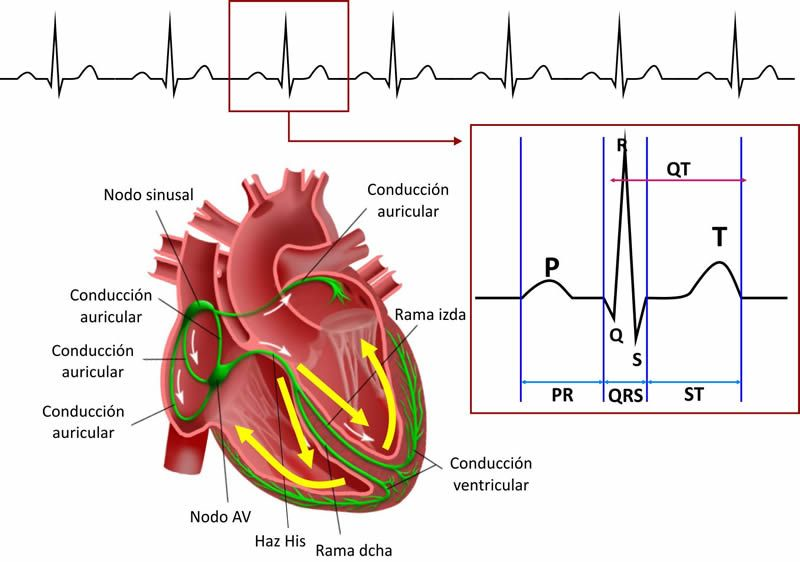
\includegraphics[width=0.9\linewidth]{_fig/sn_pulso-cardiaco.png}
	\caption{Distribución del impulso cardíaco y ondas e intervalos del electrocardiograma}
	\label{fig:sn_pulso-cardiaco}
\end{figure}

\subsection{Ejemplo de respuesta de sistema natural} %p4
En la figura \ref{fig:sn_audicion} se muestra la respuesta del sistema auditivo humano en la forma de la gráfica de sensibilidad de audición.

\begin{figure}[h]
	\centering
	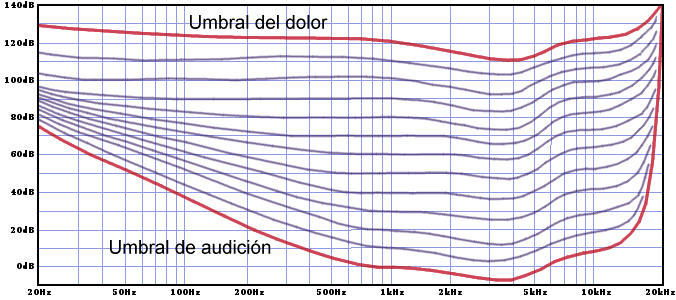
\includegraphics[width=0.9\linewidth]{_fig/sn_audicion.png}
	\caption{Umbral de dolor y umbral de audición}
	\label{fig:sn_audicion}
\end{figure}

Es decir, se requiere menos potencia de la fuente para escuchar un sonido de $3 kHz$ al cual somo más sensibles. Para escuchar un sonido de $100 Hz$ con la misma fuerza, la potencia real del sonido tiene que se mucho más grande. Las diferencias son tan grandes que se acude al uso de una escala logarítmica, con unidades en decibelios.

Si la respuesta para $1 KHz$ es $1$, la respuesta para $100 kHz$ es $0,01$. La respuesta relativa es $0.01/1$; en $dB$ es:

$20 log(0,01/1) = 20 log 10^{-2} = -40 dB$

\begin{figure}[h]
	\centering
	\includegraphics[width=0.6\linewidth]{_fig/respfreq_sch_hp.pdf}
	\caption{Circuito eléctrico}
	\label{fig:respfreq_sch_hp}
\end{figure}

\subsection{Respuesta de un sistema eléctrico} %p5

En la figura \ref{fig:respfreq_sch_hp} se muestra un circuito RC. A frecuencias bajas el condensador bloquea el paso de corriente, y se tiene $V_o = 0$. A frecuencias muy elevadas el condensador tiene una reactancia muy pequeña y $V_o = V_i$.

Para el circuito de la figura \ref{fig:respfreq_sch_hp}, se tiene:

$i = C \partial \frac{V_c}{\partial t} = C \partial \frac{V_i - V_o}{\partial t}$

$V_o = i R = C R \partial \frac{V_i - v_o}{\partial t}$

luego...

$C R \partial \frac{V_i}{\partial t} = V_o + C R \partial \frac{V_o}{dt}$

Podríamos resolver la ecuación diferencial al encontrar la respuesta natural en conjunto con la respuesta forzada de la señal de entrada para determinar $V_o$ dado $V_i$, por ejemplo si $V_i$ es una sinusoidal de frecuencia $\omega$. Analíticamente, un método más cómodo para establecer la relación entre $V_o$ y $V_i$ es por medio del análisis en el dominio $s$. La impedancia viene dada por la relación entre las variables de voltaje y corriente para un elemento:

\begin{tabular}{ccccc}
	$i = C \frac{\partial v}{\partial t}$ & $--->$ & $I = C S V$ & y & $Z = \frac{V}{I} = \frac{1}{C S}$ \\
	$v = L \frac{\partial i}{\partial t}$ & $--->$ & $V = L S I$ & y & $Z = \frac{V}{I} = L S$ \\
	$v = R i$ & $--->$ & $V = R I$ & y & $Z = \frac{V}{I} = R$ \\
\end{tabular}

La excitación del sistema es de la forma $e$.

\begin{figure}[h]
	\centering
	\includegraphics[width=0.6\linewidth]{_fig/respfreq_sch_hp_s.pdf}
	\caption{Circuito eléctrico, dominio S}
	\label{fig:respfreq_sch_hp_s}
\end{figure}

El circuito de la figura \ref{fig:respfreq_sch_hp} queda como se muestra en la figura \ref{fig:respfreq_sch_hp_s}, y nos da:

\begin{equation}\label{eqn:rse_1}
	\frac{V_i}{R + \frac{1}{CS}}=\frac{V_o}{R}
\end{equation}

\begin{equation}\label{eqn:rse_2}
	\frac{V_o}{V_i(S)} = \frac{R}{R + \frac{1}{C S}}
\end{equation}

\begin{equation}\label{eqn:rse_3}
	H(S) = \frac{V_o}{V_i(S)} = \frac{R}{R + \frac{1}{C S}}
\end{equation}

donde $H(S)$ es la función de transferencia del sistema; $H(S)$ nos determina los cambios de amplitud y de fase introducidos por el sistema donde la frecuencia de $V_o(t)$ es igual a la de $V_i(t)$.

"$S$" es un número complejo formado por una parte real y una parte imaginaria: $S = \Re + \Im\omega$

Un polo de $H(S)$, $S_p$, hace la función infinita, $H(S_p) = \infty$; mientras que un cero de $H(S)$, $S_z$, hace que la función cero, $H(S_z) = 0$. Para el caso anterior, el polo del sistema está en $S_p = \frac{-1}{R C}$, mientras que el cero es $S = 0$.

Se puede hallar la respuesta en frecuencia reemplazando $S$ por $\Im\omega$, es decir $e^{S t} = e^{\Im \omega t} = cos(\omega t) + \Im sin(\omega t)$, y variando $\omega$.

Entonces,

\begin{equation}\label{eqn:rse_4}
	\frac{V_o}{V_i}(\omega) = \frac{R}{R - \frac{\Im}{C \omega}}
\end{equation}

Un número complejo puede ser representado alternativamente por un módulo y una fase.

\begin{equation}\label{eqn:rse_5}
	H(\Im \omega) = |H(\Im \omega)| \angle H(\Im \omega)
\end{equation}

donde...

\begin{equation}\label{eqn:rse_6}
	|H(\Im \omega)| = \sqrt{\Re^2(H(\Im \omega)) + \Im^2(H(\Im \omega))}
\end{equation}

\begin{equation}\label{eqn:rse_7}
	\angle H(\Im \omega) = \tan^{-1}\frac{\Im(H(j\omega))}{\Re(H(j\omega))}
\end{equation}

Alternativamente, se puede trabajar el denominador por separado. Por ejemplo si tenemos: $\frac{1}{a+bj}$

entonces $|\frac{1}{(a+bj)}| = \frac{1}{\sqrt{a^2+b^2}}$

y $\angle (\frac{1}{(a+bj)}) = \tan^{-1} \frac{b}{a}$

De la ecuación \eqref{eqn:rse_4}:

$|\frac{V_O}{V_I} (\omega)| = \frac{R}{\sqrt{R^2+{\frac{1}{C\omega}}^2}}$

y

$\angle \frac{V_0}{V_I} (\omega) = \tan^{-1} (\frac{1}{\omega CR})$

éstas ecuaciones se grafican en la figura \ref{fig:respfreq_hp}, cambio de variable de $\omega = 2 \pi f$ para trabajar en términos de frecuencia, considere que para las figuras siguientes se ha definido $Vi=1V$, $R=10k\Omega$ y $C=1nF$:

\begin{figure}[h]
	\centering
	\subfloat[Amplitud]
	{
		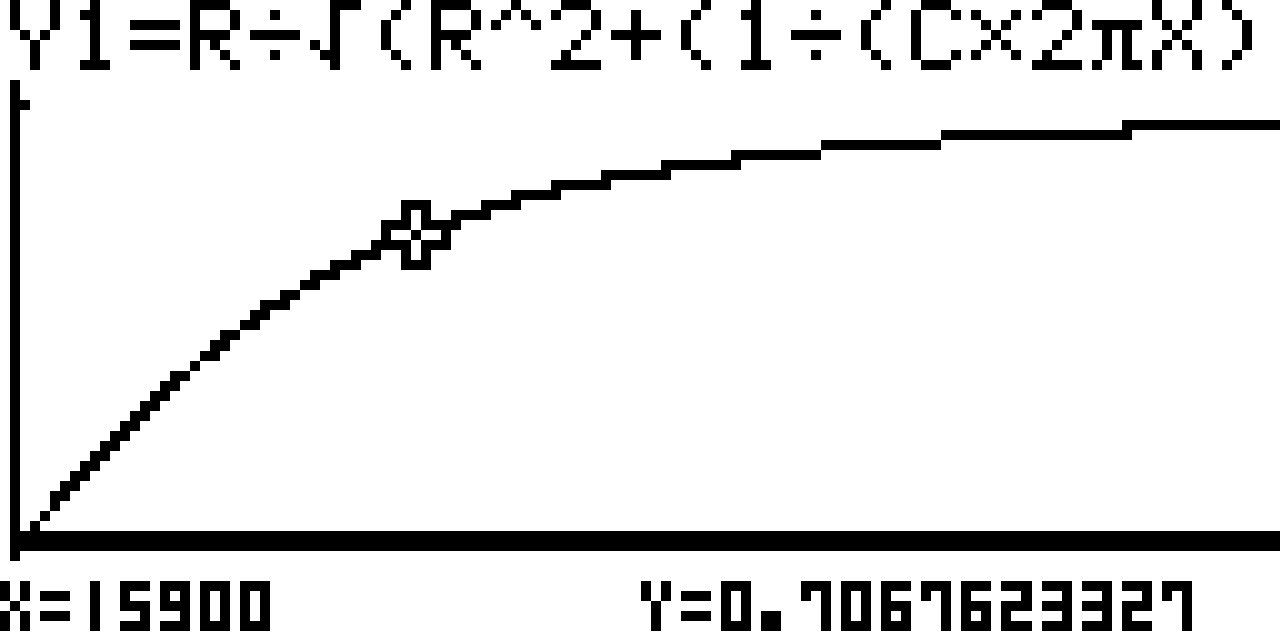
\includegraphics[width=0.4\linewidth]{_fig/respfreq_hp_abs.png}
		\label{fig:respfreq_hp_abs}
	}
	\subfloat[Angulo]
	{
		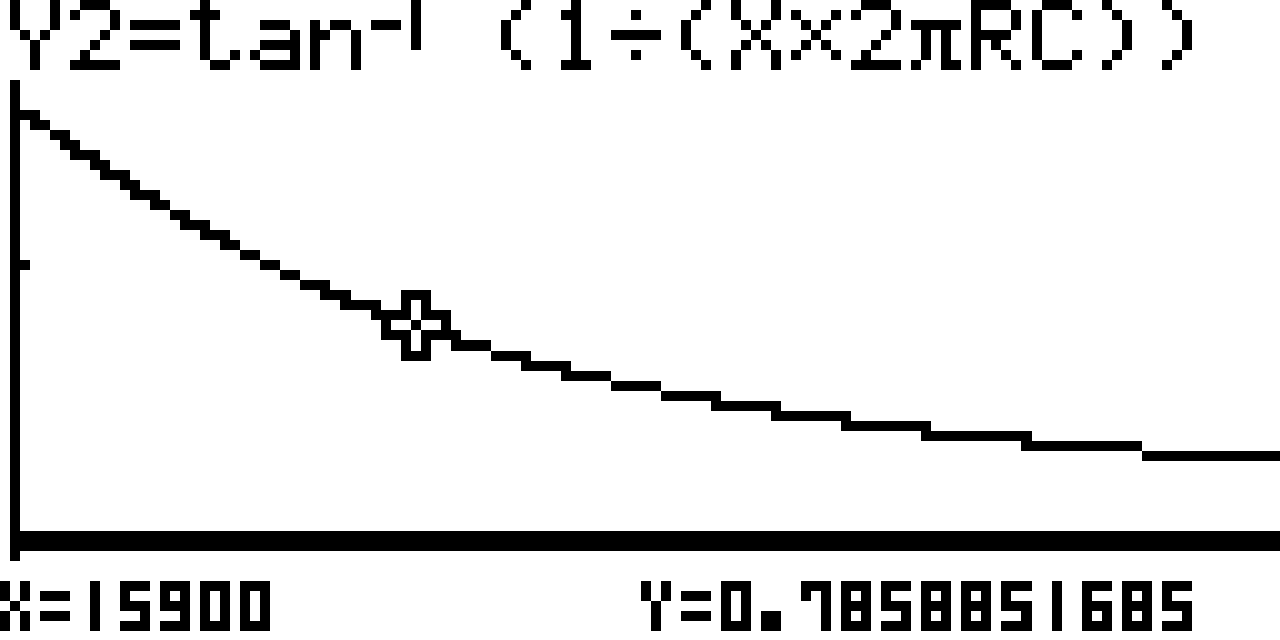
\includegraphics[width=0.4\linewidth]{_fig/respfreq_hp_ang.png}
		\label{fig:respfreq_hp_ang}
	}
	\caption{Respuesta en frecuencia, paso alto}
	\label{fig:respfreq_hp}
\end{figure}

Estas gráficas muestran la relación entre $V_O$ y $V_I$ a cualquier frecuencia. Por ejemplo, a la frecuencia $\omega=\frac{1}{2 \pi RC}$, $V_O$ tiene la $\frac{1}{\sqrt{2}}$ de amplitud de $V_I$(ver figura \ref{fig:respfreq_hp_abs}) y está desfasado $45^{\circ}$ o $\pi/4$ (ver figura \ref{fig:respfreq_hp_ang}).

\begin{figure}[h]
	\centering
	\subfloat[Gráfica $V_I$ y $V_O$]
	{
		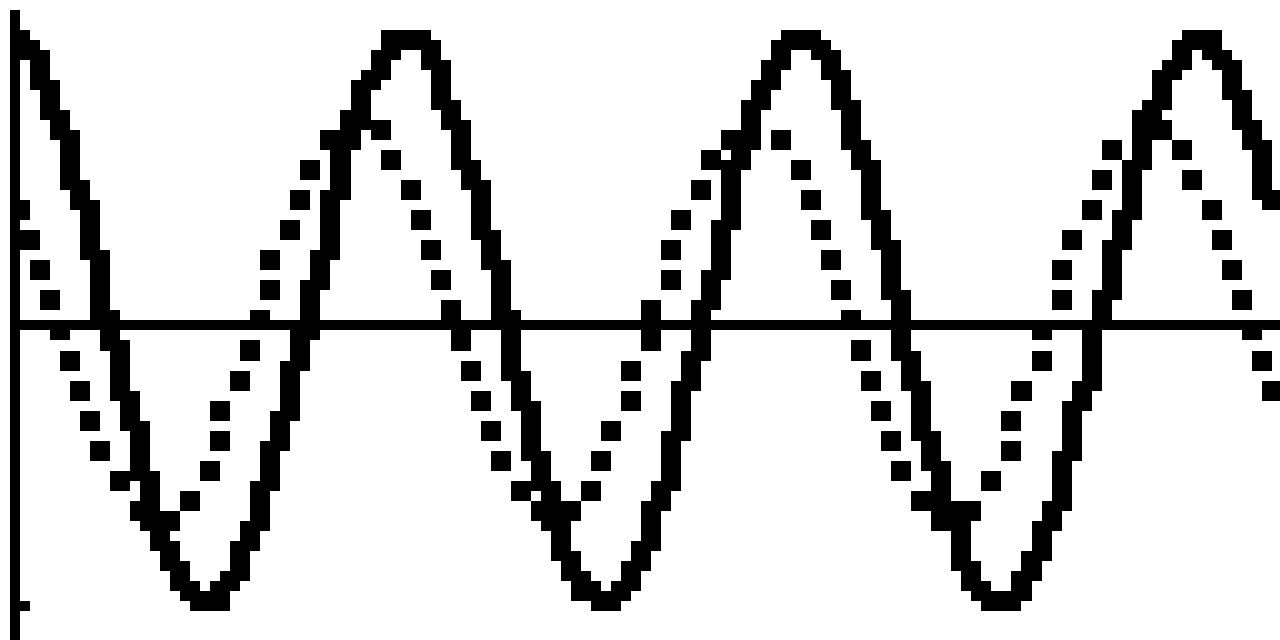
\includegraphics[width=0.4\linewidth]{_fig/respfreq_hp_vivo_plot.png}
		\label{fig:respfreq_hp_vivo_plot}
	}
	\subfloat[Ecuaciones]
	{
		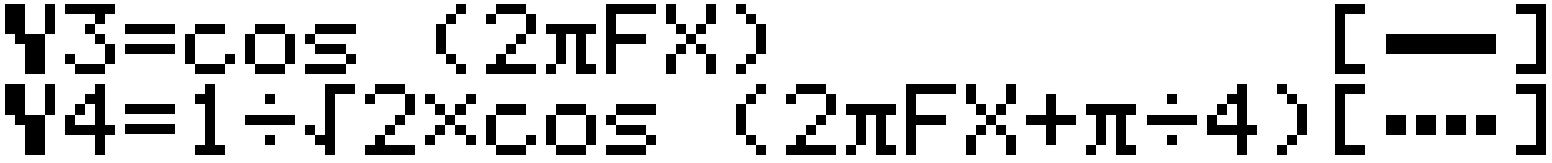
\includegraphics[width=0.4\linewidth]{_fig/respfreq_hp_vivo_eq.png}
		\label{fig:respfreq_hp_vivo_eq}
	}
	\caption{Relación entre $V_O$ y $V_I$ de la figura \ref{fig:respfreq_sch_hp} para $\omega=\frac{1}{2 \pi RC}$}
	\label{fig:respfreq_hp_vivo}
\end{figure}

La figura \ref{fig:respfreq_hp} representa un filtro paso alto: atenúa la señal de baja frecuencia, deja pasar la señal de alta frecuencia. En la figuras \ref{fig:respfreq_sch_lp} y \ref{fig:respfreq_lp} se muestra un filtro paso bajo.

\begin{figure}[h]
	\centering
	\includegraphics[width=0.6\linewidth]{_fig/respfreq_sch_hp.pdf}
	\caption{Circuito eléctrico, paso bajo}
	\label{fig:respfreq_sch_lp}
\end{figure}			

\begin{figure}[h]
	\centering
	\subfloat[Amplitud]
	{
		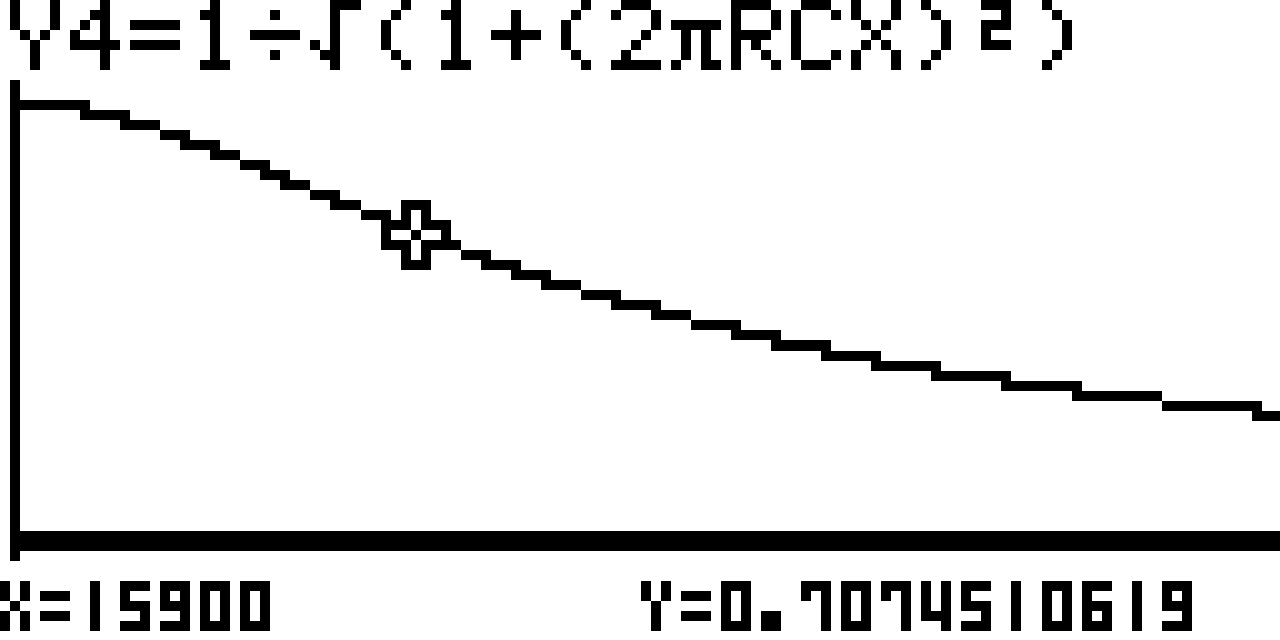
\includegraphics[width=0.4\linewidth]{_fig/respfreq_lp_abs.png}
		\label{fig:respfreq_lp_abs}
	}
	\subfloat[Angulo]
	{
		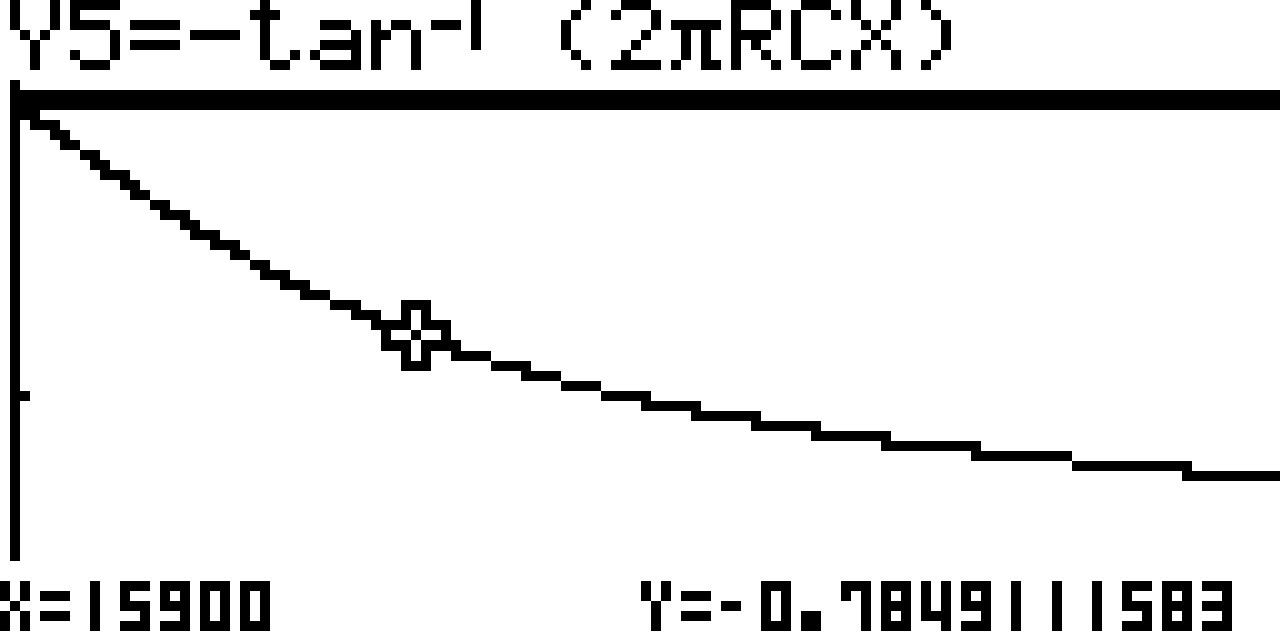
\includegraphics[width=0.4\linewidth]{_fig/respfreq_lp_ang.png}
		\label{fig:respfreq_lp_ang}
	}
	\caption{Respuesta en frecuencia, paso bajo}
	\label{fig:respfreq_lp}
\end{figure}

Bien se pueden resumir las respuestas de los filtros pasa alta y pasa baja de primer orden como se observan en las figuras \ref{fig:respfreq_summary_hp} y \ref{fig:respfreq_summary_lp}.

\begin{figure}[h]
	\centering
	\subfloat[Filtro paso alto]
	{
		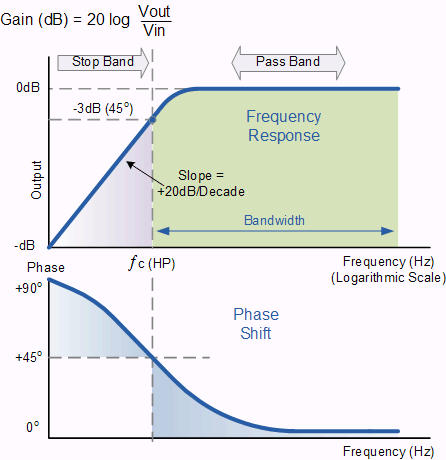
\includegraphics[width=0.4\linewidth]{_fig/respfreq_summary_hp.png}
		\label{fig:respfreq_summary_hp}
	}
	\subfloat[Filtro paso bajo]
	{
		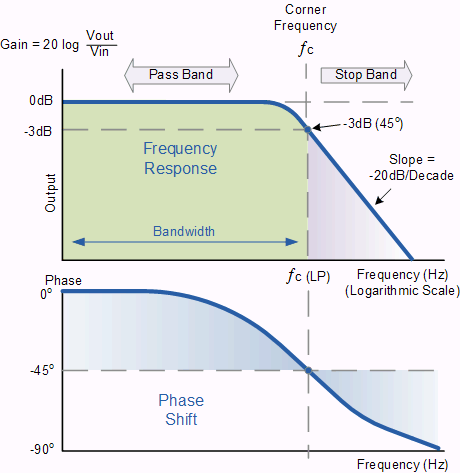
\includegraphics[width=0.4\linewidth]{_fig/respfreq_summary_lp.png}
		\label{fig:respfreq_summary_lp}
	}
	\caption{Respuesta en frecuencia, filtros de primer orden}
	\label{fig:respfreq_summary_hplp}
\end{figure}

\section{El diagrama de Bode} %p9

Los diagramas de Bode fueron ideados originalmente por el Dr. Henrik Wayne Bode mientras trabajaba para los Laboratorios Bell en la década de 1930. Se utilizan sobre todo para analizar la estabilidad de los sistemas de control, por ejemplo, al diseñar y analizar bucles de retroalimentación de la fuente de alimentación. La ventaja de utilizar el diagrama de Bode es que proporciona una forma sencilla y común de describir la respuesta de frecuencia de un sistema lineal invariante en el tiempo. Bode propuso graficar la respuesta de frecuencia en una escala logarítmica ya que de esta gráfica se podría distinguir información no fácilmente apreciable en la escala lineal.

Su motivación puede apreciarse de las gráficas de las funciones $H_1(S)$ y $H_2(S)$ en la figura \ref{fig:respfreq_bode} donde:

$H_1(S) = \frac{10}{1+\frac{S}{10}}$ y $H_2(S) = \frac{10}{(1+\frac{S}{15.625})^2}$

Las dos gráficas lucen idénticas; en particular no dejan distinguir dos diferencias importantes entre las funciones de transferencia:

\begin{enumerate}
	\item un sistema es de primer orden mientras que el otro es de segundo orden y...
	\item el valor de los polos en los dos sistemas difieren en un 50\%
\end{enumerate}

\begin{figure}[h]
	\centering
	\subfloat[$H_1(S)$]
	{
		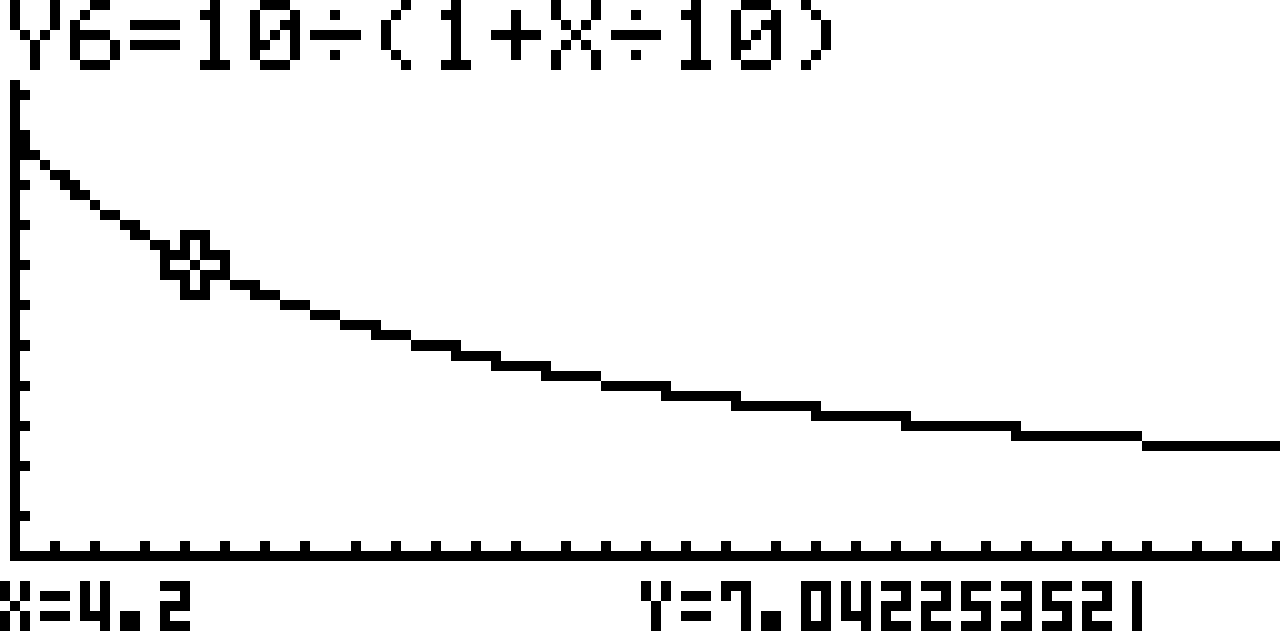
\includegraphics[width=0.4\linewidth]{_fig/respfreq_bode_h1.png}
		\label{fig:respfreq_bode_h1}
	}
	\subfloat[$H_2(S)$]
	{
		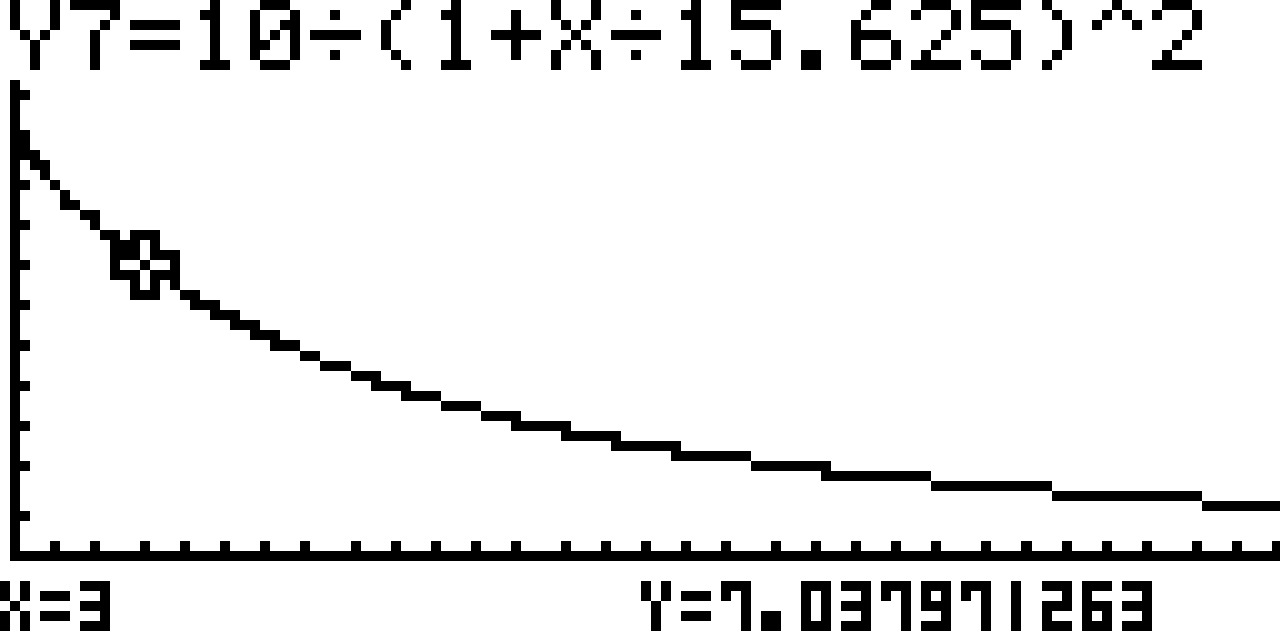
\includegraphics[width=0.4\linewidth]{_fig/respfreq_bode_h2.png}
		\label{fig:respfreq_bode_h2}
	}
	\caption{Respuestas $H_1(S)$ y $H_2(S)$}
	\label{fig:respfreq_bode}
\end{figure}

El diagrama de Bode es sencillamente la respuesta de frecuencia con la frecuencia en escala logarítmica, la magnitud en escala logarítmica, y la fase en escala lineal. Una aproximación a la curva se puede trazar a mano alzada sin necesidad de cálculos, sino en base a rectas y cambios de pendiente a las frecuencias de los polos y los ceros de la función de transferencia.

Dado una función generalizada de la forma:

\begin{equation}\label{eqn:rse_8}
	H(S) = \frac{a_mS^m + a_{m-1}S^{m-1} + ... + a_1S + q_0}{b_nS^n + b_{n-1}S^{n-1} + ... + n_1S + b_0}
\end{equation}

podemos expresarla para distinguir los ceros, los polos y una constantes:

\begin{equation}\label{eqn:rse_9}
	H(S) = a \frac{(S-Z_1)(S-Z_2) ... (S-Z_m)}{(S-p_1)(S-p_2) ... (S-p_n)}
\end{equation}

el módulo de $H(S)$ viene dado por:

\begin{equation}\label{eqn:rse_10}
	|H(S)| = a \frac{|S-Z_1||S-Z_2| ... |S-Z_m|}{|S-p_1||S-p_2| ... |S-p_n|}
\end{equation}

si ahora tomamos el logaritmo de ésta función y lo multiplicamos por $20$ se convierte en la forma apropiada para el Diagrama de Bode del módulo:

\begin{equation}\begin{split}\label{eqn:rse_11}
		20log|H(S)| = 20log|a| + 20log|S-Z_1| + 20log|S-Z_2| ... + 20log|S-Z_m| \\
		- 20log|S-P_1| - 20log|S-P_2| ... - 20log|S-P_n|
\end{split}\end{equation}

se hace notar como el producto de funciones se ha convertido en la suma de funciones para dar el total.

La fase de $H(S)$ se encuentra en la siguiente expresión:

\begin{equation}\begin{split}\label{eqn:rse_12}
		\angle|H(S)| = \angle a + \angle(S-Z_1) + \angle(S-Z_2) ... + \angle(S-Z_m) \\
		- \angle(S-P_1) - \angle(S-P_2) ... - \angle(S-P_n)
\end{split}\end{equation}

nuevamente la contribución de cada raíz y la constante se suma para obtener la total.

En la figura \ref{fig:respfreq_db_cero} se traza el Diagrama de Bode del módulo y la fase que contribuye un cero. Para el cero expresado de la forma $(1+\frac{S}{\omega})$, el módulo arranca a un nivel de $0 dB$ a frecuencias bajas, sube a $3 dB$ a la frecuencia del cero y eventualmente aumenta en forma proporcional a $\omega$, que en la escala logarítmica-logarítmica del Bode se representa con una pendiente de $20 dB$ por década (factor de diez) de frecuencia. La fase del cero arranca en $0^{\circ}$ a frecuencias bajas, sube a $5,17^{\circ}$ a una frecuencia 10 veces por debajo del cero, para por $45^{\circ}$ a la frecuencia del cero, llega a $84.83^{\circ}$ a una frecuencia 10 veces mayor que el cero hasta eventualmente llegar a un valor final de $+90^{\circ}$. Adicionalmente se dibuja asíntotas a las curvas reales. Hay varias formas de aproximar ésta curva real con rectas. La que se muestra aproxima la función $0^{\circ}$ hasta que la frecuencia $\frac{\omega_Z}{10}$, de allí subo con una recta de $\frac{45^{\circ}}{decada}$ en la escala lineal-logarítmica, para por $45^{\circ}$ a la frecuencia $\omega_Z$ hasta llegar a un valor final de $90^{\circ}$ a $10 \omega_Z$.

\begin{figure}[h]
	\centering
	\subfloat[Módulo]
	{
		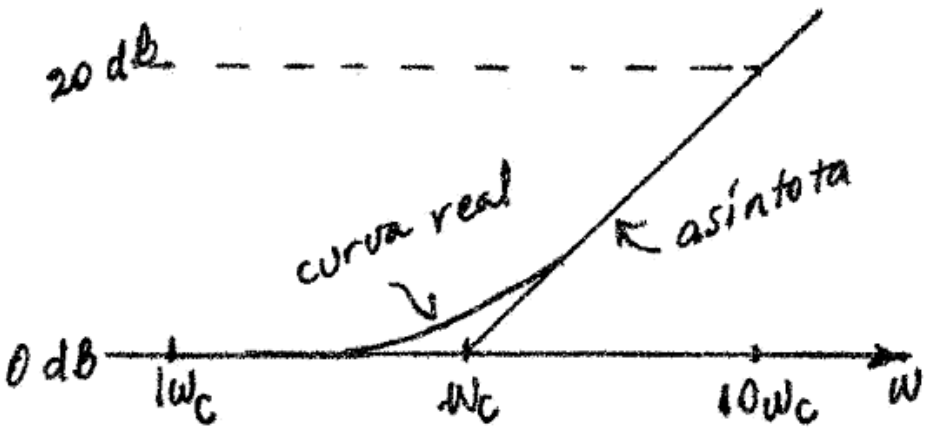
\includegraphics[width=0.4\linewidth]{_fig/respfreq_db_cero_modulo.png}
		\label{fig:respfreq_db_cero_modulo}
	}
	\subfloat[Fase]
	{
		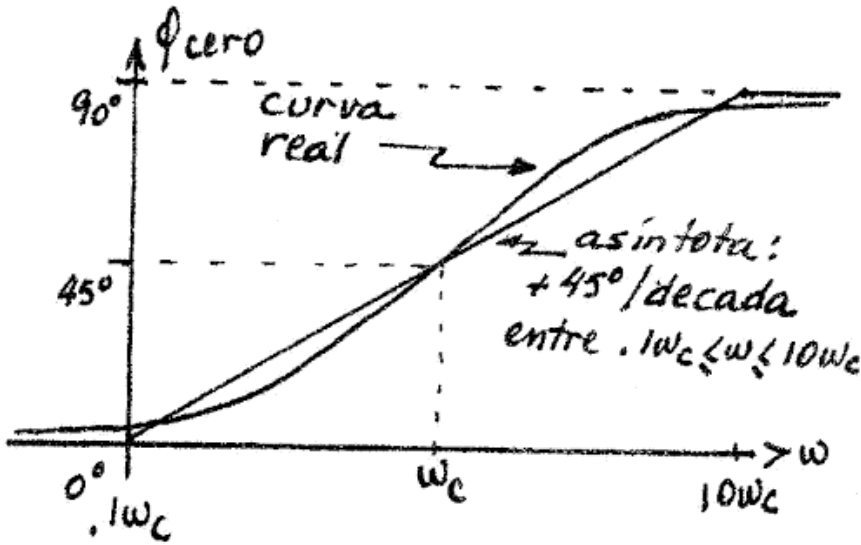
\includegraphics[width=0.4\linewidth]{_fig/respfreq_db_cero_fase.png}
		\label{fig:respfreq_db_cero_fase}
	}
	\caption{Diagrama de Bode de un Cero}
	\label{fig:respfreq_db_cero}
\end{figure}

En la figura \ref{fig:respfreq_db_polo} se traza el Diagrama de Bode del módulo y la fase que contribuye un polo. Se hace notar idénticas a las curvas del cero pero en sentido negativo. Para el polo expresado de la forma $1+\frac{S}{\omega}$, el módulo arranca a un nivel de $0 dB$ a frecuencias bajas, baja a $3 dB$ a la frecuencia del polo y eventualmente disminuye en forma proporcional a $\omega$, que en la escala logarítmica-logarítmica del Bode se representa con una pendiente de $-20 dB$ por década (factor de diez) de frecuencia. La fase del polo arranca en $0^{\circ}$ a frecuencias bajas. Baja a $-5,17^{\circ}$ a una frecuencia 10 veces por debajo del polo, pasa por $-45^{\circ}$ a la frecuencia del polo, llega a $84,83^{\circ}$ a una frecuencia 10 veces mayor que el polo hasta eventualmente llegar a un valor final de $-90^{\circ}$. Nuevamente se dibuja asíntotas a las curvas reales. La aproximación a esta curva real con rectas consta de un valor de $0$ hasta la frecuencia $\omega_P/10$, de allí baja con una recta de $\frac{-45^{\circ}}{decada}$ en la escala lineal-logarítmica, pasa por $-45^{\circ}$ a la frecuencia $\omega_P$ hasta llegar a un valor final de $-90^{\circ}$ a $10 \omega_P$.

\begin{figure}[h]
	\centering
	\subfloat[Módulo]
	{
		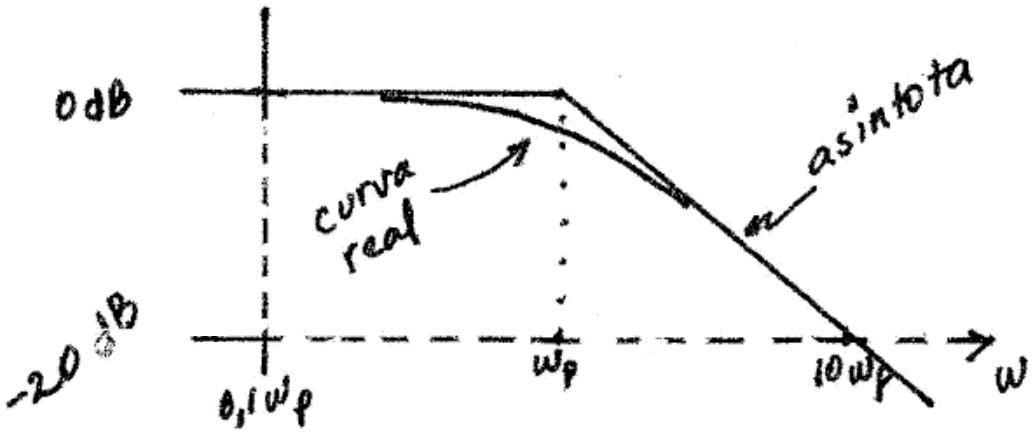
\includegraphics[width=0.4\linewidth]{_fig/respfreq_db_polo_modulo.png}
		\label{fig:respfreq_db_polo_modulo}
	}
	\subfloat[Fase]
	{
		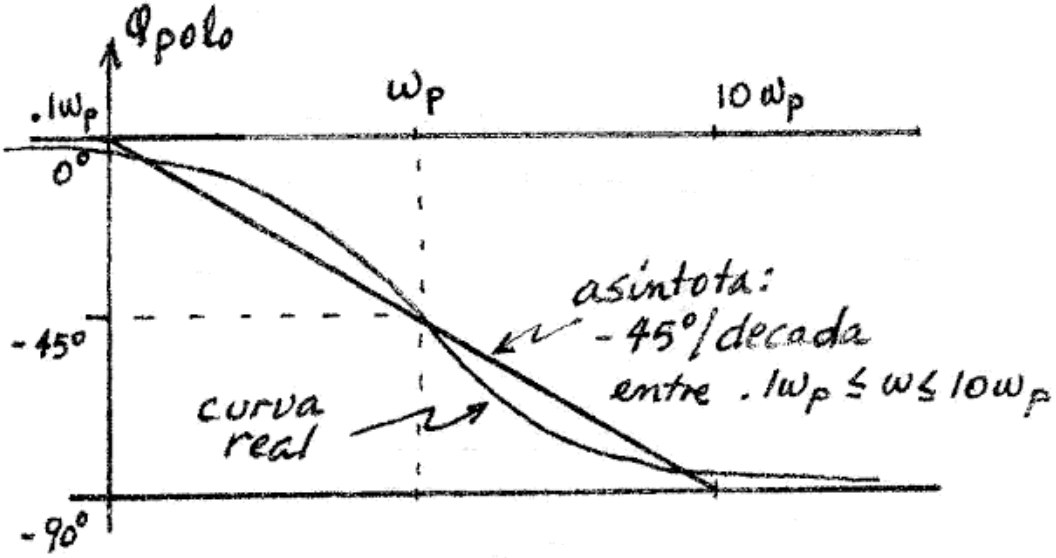
\includegraphics[width=0.4\linewidth]{_fig/respfreq_db_polo_fase.png}
		\label{fig:respfreq_db_polo_fase}
	}
	\caption{Diagrama de Bode de un Polo}
	\label{fig:respfreq_db_polo}
\end{figure}

Finalmente la constante contribuirá con un nivel de $20 log k$ al módulo, es decir, será constante, y su contribución a la fase será $0^{\circ}$ en caso de tratarse de un valor real y positivo, ó de $-180^{\circ}$ en caso de una constante real y negativa.

Por ejemplo, en la figura \ref{fig:respfreq_bode_h12_resp} se trazan los Diagramas de Bode de las funciones de transferencia con las cuales iniciamos esta sección:

$H_1(S) = \frac{10}{1+\frac{S}{10}}$ y $H_2(S) = \frac{10}{(1+\frac{S}{15.625})^2}$

Se comparan con la figura \ref{fig:respfreq_bode} y se puede apreciar mayor cantidad de información del sistema que puede obtenerse con la gráficas. Además las rectas que aproximan la curva real se trazan directamente sin necesidad de cálculos. El Diagrama de Bode es la forma preferida para el trazo de la respuesta en frecuencia de sistemas. Es particularmente útil para reflejar la atenuación exacta en la banda de atenuación.

\begin{figure}[h]
	\centering
	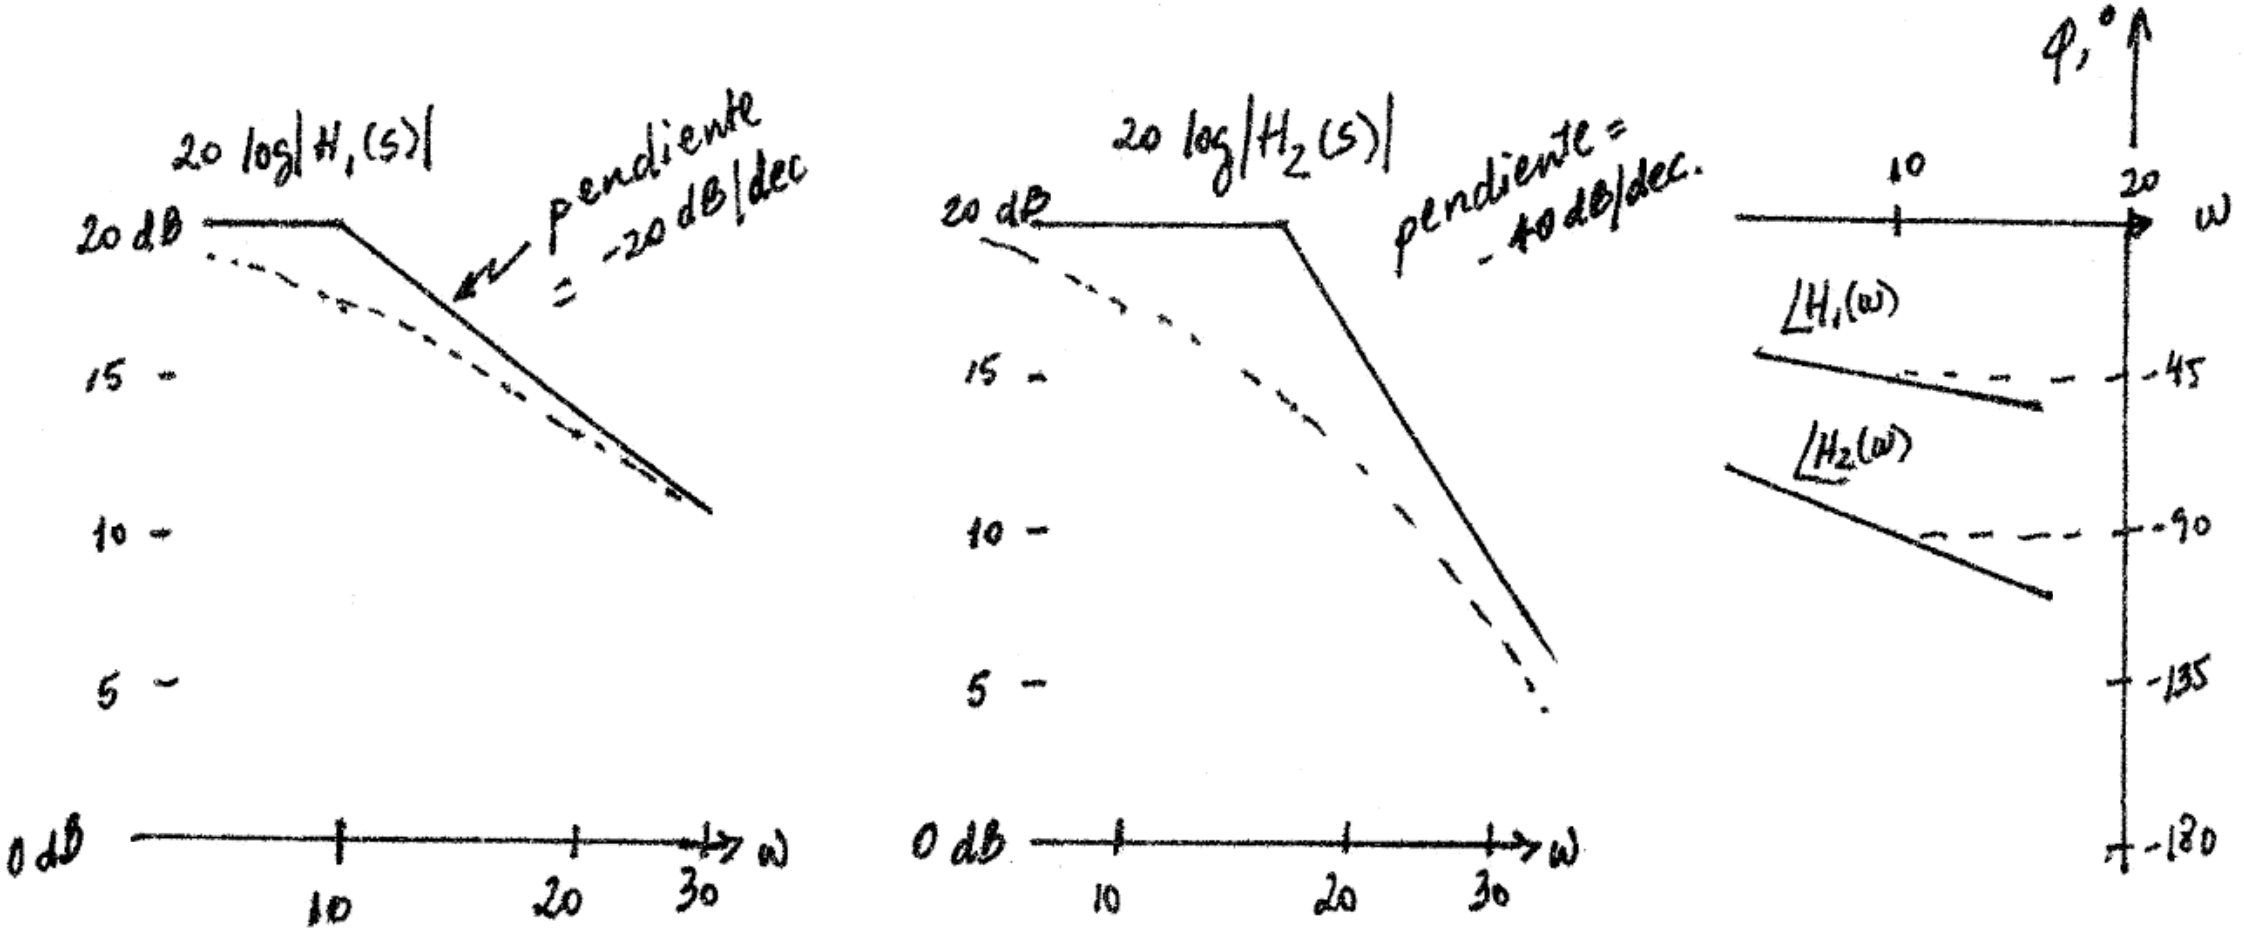
\includegraphics[width=0.9\linewidth]{_fig/respfreq_bode_h12_resp.png}
	\caption{Respuestas en Diagrama de Bode de $H_1(S)$ y $H_2(S)$}
	\label{fig:respfreq_bode_h12_resp}
\end{figure}

\section{Respuesta de los amplificadores} %p13

Existe una clase general de circuitos conocidos como amplificadores de banda ancha que se caracterizan por tener una ganancia constante en un rango relativamente ancho de frecuencias. Dentro de esta clase existen dos tipos: el amplificador de $DC$ y el amplificador acoplado capacitivamente.

En el amplificador DC, la señal es acoplada directamente entre etapas; la respuesta de frecuencia es como la que aparece en la Figura \ref{fig:respfreq_amp-dc}. 
El amplificador tiene una ganancia constante para un rango relativamente amplio de frecuencias, a partir de DC.

\begin{figure}[h]
	\centering
	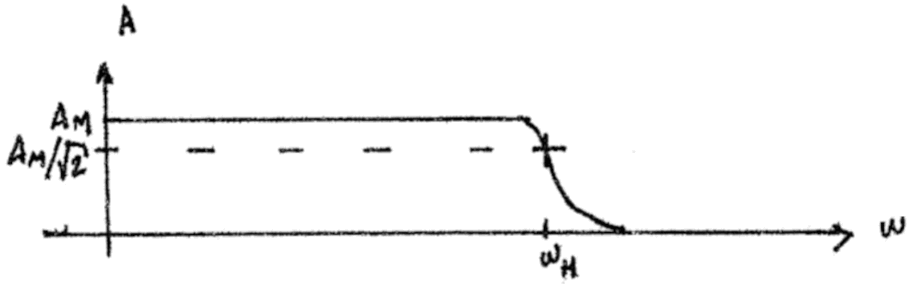
\includegraphics[width=0.9\linewidth]{_fig/respfreq_amp-dc.png}
	\caption{Respuesta de frecuencia del amplificador DC}
	\label{fig:respfreq_amp-dc}
\end{figure}

La respuesta del amplificador de banda ancha acoplado capacitivamente se muestra en la Figura \ref{fig:respfreq_amp-dc_acomple-c}. Nuevamente hay un rango relativamente amplio de frecuencias en que la ganancia es constante con la diferencia de que no amplifica corriente continua.

\begin{figure}[h]
	\centering
	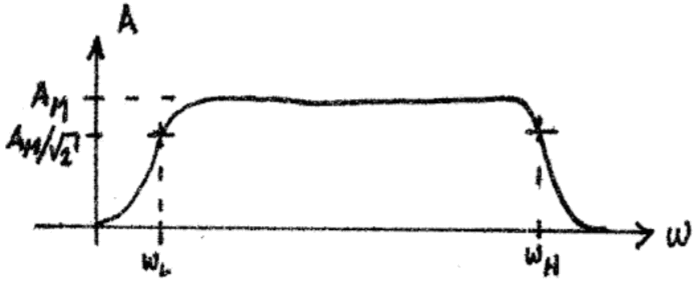
\includegraphics[width=0.9\linewidth]{_fig/respfreq_amp-dc_acomple-c.png}
	\caption{Respuesta de frecuencia del amplificador acoplado capacitivamente}
	\label{fig:respfreq_amp-dc_acomple-c}
\end{figure}

Para la clase de circuito amplificador de banda ancha, una caracterización se distingue por su ganancia a frecuencias medias, $A_m$, y las dos frecuencias esquinas: la frecuencia de corte baja, $f_L$, y la frecuencia de corte alta, $f_H$. Las frecuencias de corte se definen como las frecuencias a las cuales el módulo de la ganancia ha bajado a $1/\sqrt{2}$ de su valor máximo. Alternativamente, se conocen como las frecuencias de media potencia.

Es conveniente considerar la función de transferencia compuesta de la siguiente forma:

\begin{equation}
	A(s) = A_M F_L(s) F_H(s)
\end{equation}

tal como se muestra en la Figura \ref{fig:fig3}. \( A_M \) es la ganancia constante a frecuencias medias; se calcula con los condensadores de acoplamiento y de puente cortocircuitados y sin considerar las limitaciones de frecuencia de los dispositivos. \( F_L(s) \) es la función de \( s \) que encierra todas las dependencias de frecuencia del amplificador a frecuencias bajas y que se caracteriza por un filtro paso alto, es decir:

\[ 
F_L (\omega) \cong 1 \text{ para } \omega \gg \omega_L, \quad F_L(f_L) = 1/\sqrt{2} 
\]

\begin{equation}
	A(s) \cong A_M F_H (s) \text{ para } \omega \gg \omega_L \quad (1.14) 
\end{equation}

\( F_H (s) \) es la función de \( s \) que incluye todos los efectos que afectan la respuesta de frecuencia del amplificador a frecuencias altas y que se caracteriza por un filtro paso bajo, es decir:

\[ 
F_H (\omega) \cong 1 \text{ para } \omega \ll \omega_H, \quad F_H(f_H) = 1/\sqrt{2} 
\]

y

\begin{equation}
	A(s) \cong A_M F_L (s) \text{ para } \omega \ll \omega_H \quad (1.15) 
\end{equation}

\( F_L (s) \) es de la siguiente forma:

\begin{figure}[h]
	\centering
	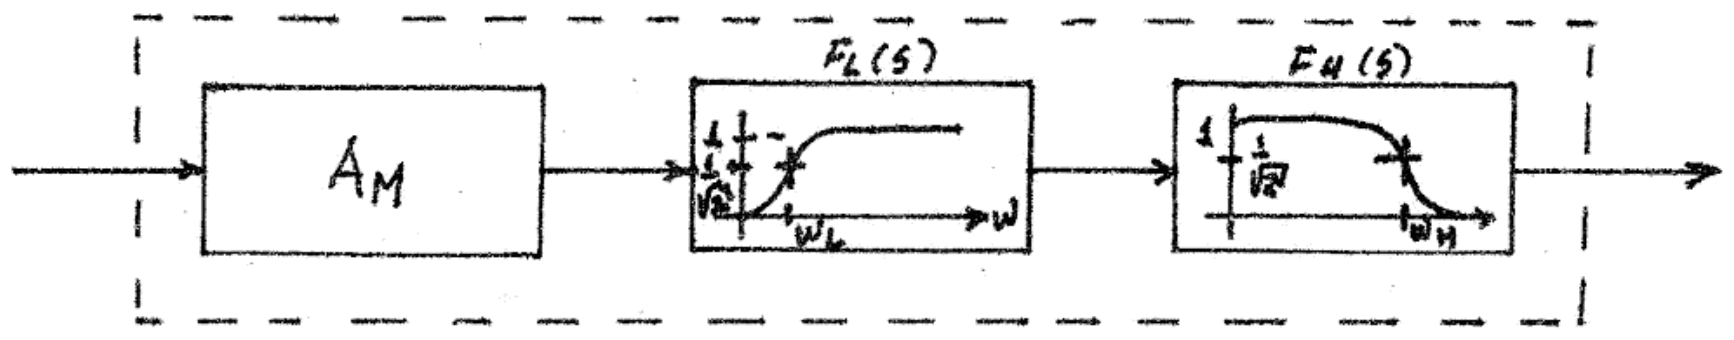
\includegraphics[width=0.9\linewidth]{_fig/respfreq_forma-fl.png}
	\caption{Forma de \( F_L (s) \)}
	\label{fig:respfreq_forma-fl}
\end{figure}

\begin{equation} \label{respfreq_fl}
	F_L(s) = \frac{(s + w_{z1})(s + w_{z2}) \cdots (s + w_{zpn})}{(s + w_{p1})(s + w_{p2}) \cdots (s + w_{pm})}
\end{equation}

donde los \( w_{z1} < w_{p1} \), es decir existen parejas de cero con polo donde la frecuencia del polo es mayor que la frecuencia del cero (filtro paso alto). Además para la relación de la ecuación \ref{respfreq_fl}, cuando \( s \gg w_L \), entonces \( F_L(s) \leq 1 \).

Mientras que \( F_H(s) \) es de la forma:

\begin{equation}
	F_H(s) = \frac{(sT_{z1} + 1)(sT_{z2} + 1)}{(sT_{p1} + 1)(sT_{p2} + 1)} \cdots \frac{(sT_{pn} + 1)}{(sT_{pn} + 1)}
\end{equation}

donde \( T_{p1} > T_{z1} \), es decir la frecuencia del polo es menor que la frecuencia del cero (filtro paso bajo) y generalmente \( T_{z2} = 0 \), y cuando \( s \ll w_H \), \( F_H(s) \leq 1 \).

\section{Análisis de un circuito con FET} %p16

En la Figura \ref{fig:respfreq_amp-fet} se muestra un amplificador FET fuente común con su circuito de polarización, su condensador de acoplamiento a la entrada, \( C_C \), y el condensador de puenteo de la resistencia de la fuente (\( C_S \)).

\begin{figure}[h]
	\centering
	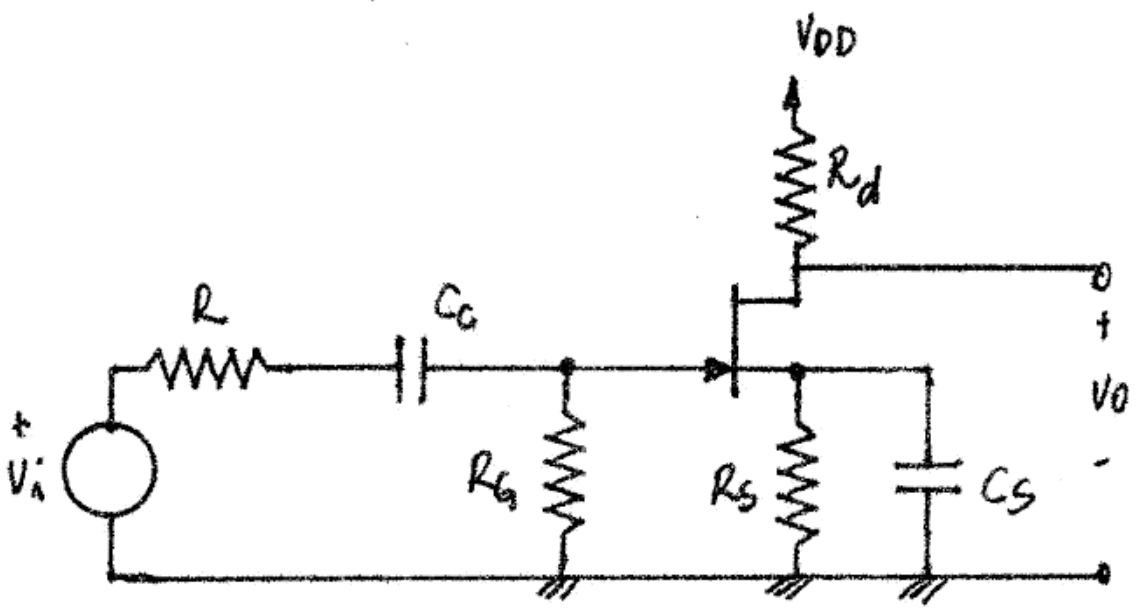
\includegraphics[width=0.9\linewidth]{_fig/respfreq_amp-fet.png}
	\caption{Amplificador FET}
	\label{fig:respfreq_amp-fet}
\end{figure}

El modelo apropiado del FET para realizar nuestro análisis frecuencial se muestra en la Figura \ref{fig:respfreq_modelo-fet}. Además de la fuente de Corriente controlada, \( g_m \psi_{gs} \), y la resistencia de salida, \( r_d \), se incluye capacitancias entre los bornes externos del dispositivo. Para transistores de pequeña señal, estas capacitancias son del orden de los $pF$.

\begin{figure}[h]
	\centering
	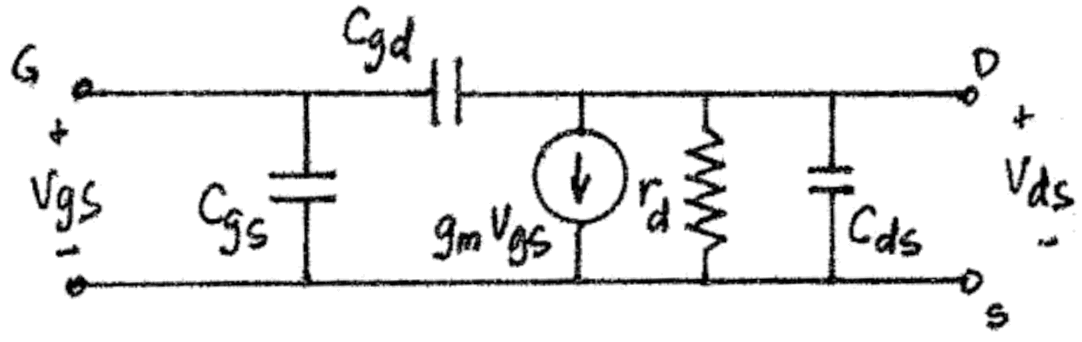
\includegraphics[width=0.9\linewidth]{_fig/respfreq_modelo-fet.png}
	\caption{Modelo del FET}
	\label{fig:respfreq_modelo-fet}
\end{figure}

La forma rutinaria de realizar el análisis frecuencial de este circuito reemplazaría el FET de la Figura \ref{fig:respfreq_amp-fet} con el modelo del FET de la Figura \ref{fig:respfreq_modelo-fet}, resultando así un circuito con 5 condensadores. Es decir, la función de transferencia sería aparentemente una función en $s$ de quinto orden! Y eso que apenas estamos considerando un circuito de un solo transistor. Para circuitos más grandes, cada transistor implica adicionar 3 capacitancias más, sin incluir los condensadores correspondientes de acoplamiento y de puenteo. En fin nos queda por delante un análisis complicado dado lo pequeño que es el circuito.

Como una primera simplificación del análisis, vamos a limitarnos a rangos determinados de frecuencia. Esto ya se hizo cuando se calculó la ganancia \( A_M \) del circuito a frecuencias medias. Haremos un análisis de baja frecuencia en donde no tomaremos en cuenta las capacitancias internas del FET ya que no afectan apreciablemente la respuesta a frecuencias bajas y medias. Y haremos un análisis de alta frecuencia donde no tomaremos en cuenta los condensadores que solo afectan la respuesta a bajas frecuencias.

Antes que nada se debe determinar el punto de operación en continua del circuito, con las ecuaciones:

\begin{equation}
	V_{GS} = V_G - I_D R_S
\end{equation}

\begin{equation}
	I_D = I_{DSS} \left(1 - \frac{V_{GS}}{V_P}\right)^2
\end{equation}

De esta forma podremos calcular el parámetro

\[
g_m = \frac{\partial I_D}{\partial V_{GS}}
\]

Entonces para baja frecuencia se analiza el circuito que se muestra en la Figura \ref{fig:respfreq_modelo-fet-lf}; \( r_d \) no se toma en cuenta por ahora para simplificar el análisis y considerando que su efecto es despreciable. Para mayor precisión se tomaría en cuenta.

\begin{figure}[h]
	\centering
	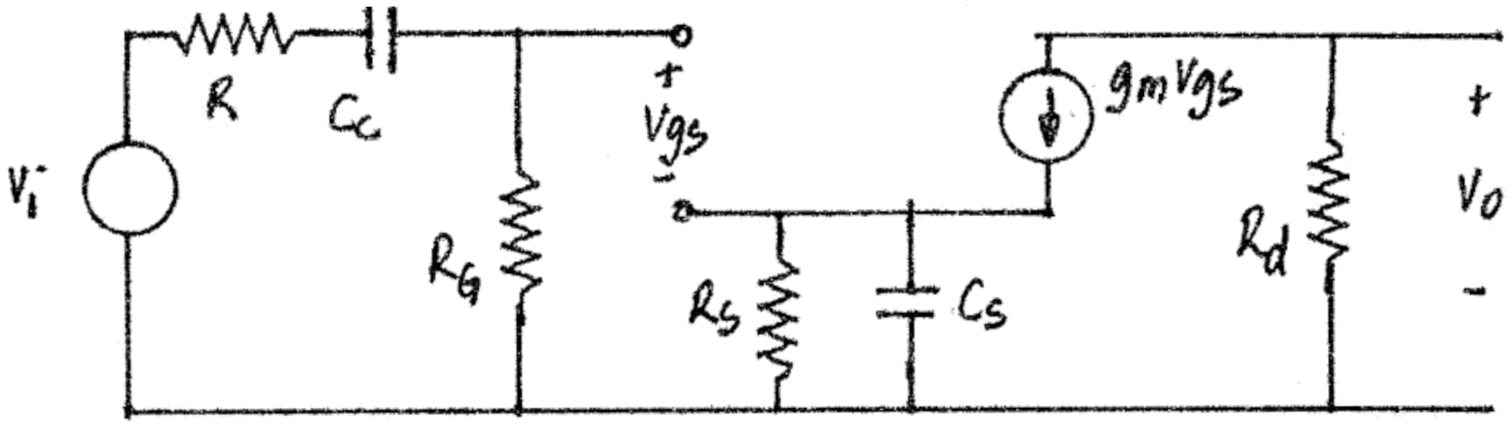
\includegraphics[width=0.9\linewidth]{_fig/respfreq_modelo-fet-lf.png}
	\caption{Modelo del FET para baja frecuencia}
	\label{fig:respfreq_modelo-fet-lf}
\end{figure}

Hallaremos \( \frac{v_o}{v_i'} \) por partes:

\begin{equation}
	\frac{v_o}{v_i'} = \left(\frac{v_o}{v_g}\right) \left(\frac{v_g}{v_i'}\right)
\end{equation}

De la malla de entrada se halla \( \frac{v_g}{v_i'} \):

\[
\frac{v_g}{v_i} = \frac{R_g}{R_g + \frac{1}{sC_C} + R}
\]

\begin{equation} \label{respfreq_vg-vi}
	\frac{v_g}{v_i} = \left(\frac{R_g}{R_g + R}\right) \frac{s}{s + \frac{1}{C_C(R + R_g)}}
\end{equation}

es decir introduce un cero en el origen y un polo a la frecuencia \( -\frac{1}{C_C(R + R_g)} \). Para hallar \( \frac{v_o}{v_g} \), tenemos las siguientes ecuaciones:

\begin{equation}
	v_o = -g_m v_{gs} R_d
\end{equation}

\begin{equation}
	v_{gs} = v_g - v_d
\end{equation}

\begin{equation}
	v_o = -g_m V_{gs} \left( R_s \parallel \frac{1}{C_s s} \right)
\end{equation}

Luego,

\begin{equation} \label{respfreq_vo-vg}
	\frac{v_o}{v_g} = \frac{-g_m R_d \left( s + \frac{1}{R_s C_s} \right)}{s + \frac{1 + 9m R_s}{C_s R_s}}
\end{equation}

Esta parte del circuito nos contribuye un cero en $-1/R_s C_s$, y un polo en $-\frac{1 + 9m R_s}{C_s R_s}$. La relación global es el producto de la ecuación \ref{respfreq_vg-vi} por la ecuación \ref{respfreq_vo-vg}:

\begin{equation}
	\frac{v_o}{v_i} = -\frac{g_m R_d R_q}{R_d + R} \left( \frac{s \left( s + \frac{1}{R_s C_s} \right)}{\left( s + \frac{1}{C_s (R + R_q)} \right) \left( s + \frac{1}{4cm R_s} \right)} \right)
\end{equation}

Esta función tiene la forma $A_M F_L(s)$, donde:

\begin{equation} \label{respfreq_exp_a_m}
	A_M = -\frac{g_m R_d R_q}{R_G + R}
\end{equation}

es la ganancia a frecuencias medias, y

\begin{equation} \label{respfreq_fl-gain-mf}
	F_L(s) = \frac{s \cdot \left( s + \frac{1}{R_s C_s} \right)}{\left( s + \frac{1}{C_s (R + R_q)} \right) \left( s + \frac{1}{4cm R_s} \right)}
\end{equation}

incluye todas las variaciones de frecuencia de la función global para frecuencias bajas. Afortunadamente en este circuito los condensadores se encuentran en mallas independientes de modo que nos resulta expresiones sencillas para las raíces.

Ahora hallaremos la relación $\frac{v_o}{v_i}$ para alta frecuencia. Se cortocircuitan los condensadores de baja frecuencia y nos queda por analizar el circuito que se muestra en la Figura \ref{fig:respfreq_relacion-vo-vi}.

\begin{figure}[h]
	\centering
	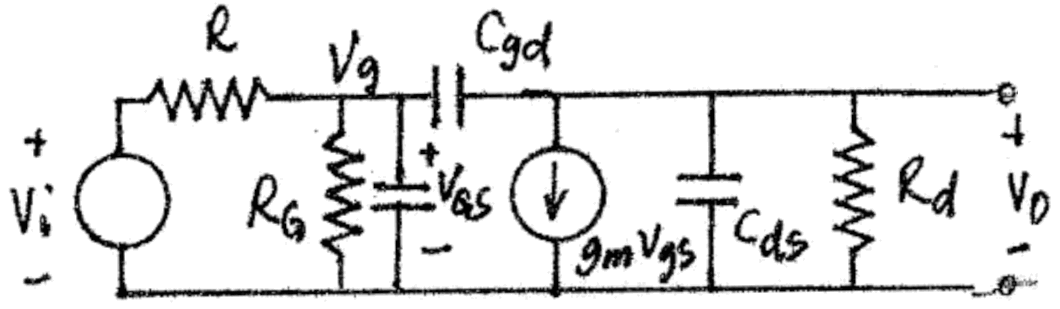
\includegraphics[width=0.9\linewidth]{_fig/respfreq_relacion-vo-vi.png}
	\caption{Modelo del FET para baja frecuencia}
	\label{fig:respfreq_relacion-vo-vi}
\end{figure}

Tenemos las siguientes ecuaciones de nodo:

\begin{equation}
	v_g \left( \frac{1}{R} + \frac{1}{R_q} + s C_{\mathrm{gs}} + s C_{\mathrm{gd}} \right) - v_o s C_{\mathrm{gd}} = \frac{V_i}{R}
\end{equation}

\begin{equation}
	v_g (g_m - sC_{gd}) + v_0(sC_{gd} + sC_{dS} + \frac{1}{R_d}) = 0
\end{equation}

de donde se obtiene:

%\[
%\frac{v_o}{v_i} = \frac{\left(-g_m - sC_{gd}\right)/{r}}{s^2\left( C_{ds} \left( C_{gs} + C_{gd} \right) + C_{gd}C_{gs} \right) + s \left( \left( \frac{1}{R} + \frac{1}{R_g} \right) \left( C_{ds} + C_{gd} + C_{gd}g_m \right) \right)} + \frac{1}{R_d} \left( \frac{1}{R} + \frac{1}{R_g} \right)
%\]

\begin{equation} \label{respfreq_vo-vi-gain-mf}
	\frac{v_o}{v_i} = \frac{\frac{-g_m R_d R_G}{R+R_G} \left(1-\frac{C_{gd}}{g_m} \right) }{ s^2 \left[ \frac{C_{ds}\left(C_{gs}+C_{gd}\right)+C_{gd}C_{gs}}{\frac{1}{R_d}\left(\frac{1}{R}+\frac{1}{R_g} \right)}\right]+s\left[R_d\left(C_{ds}+C_{gd}\right)+\frac{C_{gd}g_{m}R_d}{\frac{1}{R}+\frac{1}{R_g}} \right] + 1}
\end{equation}

Esta expresión está de la forma \(p_{ij}(s)\), donde:

\[
A_{M} = -\frac{g_m R_d R_G}{R + R_G}
\]

tiene la misma expresión de la ecuación \ref{respfreq_exp_a_m}, y

\begin{equation} \label{respfreq_funcion-transferencia}
	F_H(s) = \frac{1 - \frac{sC_{gd}}{g_M}}{s^2 \left[ \frac{C_{ds}\left(C_{gs}+C_{gd}\right)+C_{gd}C_{gs}}{\frac{1}{R_d}\left(\frac{1}{R}+\frac{1}{R_G}\right)} \right] + s\left[ R_d\left(C_{ds}+C_{gd}\right)+\frac{C_{gd}g_{m}R_{d}}{\frac{1}{R}+\frac{1}{R_{G}}} \right] + 1}
\end{equation}

La ganancia a frecuencias medias es lo que queda de la ecuación \ref{respfreq_vo-vi-gain-mf} para \(s\) relativamente pequeña. La ecuación \ref{respfreq_vo-vi-gain-mf} es una función de segundo orden cuyos polos pueden resolverse utilizando la solución cuadrática. No queda una función de tercer orden pues las tres capacitancias forman un lazo. Lo que sí puede apreciarse es que los polos no son funciones simples de condensadores individuales, ya que estos interactúan.

Ahora podemos unir los resultados de las ecuaciones \ref{respfreq_fl-gain-mf} y \ref{respfreq_vo-vi-gain-mf} para plantear a continuación la función de transferencia total del circuito de la Figura \ref{fig:respfreq_amp-fet}:

\begin{equation}
	\frac{v_o}{v_i}= \frac{-g_m R_d R_G}{R_G + R} F_{L}(S) F_{H} (S)
\end{equation}

\subsubsection{Ejemplo 1} \label{respfreq_ejm1}

Para el circuito de la Figura \ref{fig:respfreq_amp-fet} se tiene los siguientes valores: \(R_G = 1M\Omega \), \(R = 100k\Omega \), \(R_d = 2.2k\Omega\), \(R_s = 1k\Omega\), \(V_{DD} = 10V\), \(C_c = 0.1\mu F\), \(C_s = 10\mu F \). Para el FET se tiene \(I_{DSS} = 4mA\), \( V_p = -2V \), \( C_{gd} = 2pF \), \( C_ds = 3pF \), \( C_{gs} = 1pF \).

\textbf{a)} Hallar la función de transferencia del circuito, que corresponde a la ecuación \ref{respfreq_funcion-transferencia}.

\textbf{b)} Trazas el Diagrama de Bode correspondiente.

\textbf{Solución:}

\textbf{a)} Punto de operación: \( V_{gs} = -1V \), \( I_D = 1mA \), \( g_m = 2 mmho \)

\[
A_M = -4
\]

\[
F_L(s) = \frac{s(s + 100)}{(s + 9.09)(s + 300)}
\]

\[
F_H(s) = \frac{(1 - 10^{-9}s)}{(7.34 \times 10^{-7}s + 1)(2.72 \times 10^{-9}s + 1)}
\]

Con lo que la función global queda:
\[
\frac{v_o}{v_i} = \frac{-4s(s + 100)(1 - 10^{-9}s)}{(s + 9.09)(s + 300)(7.34 \times 10^{-7}s + 1)(2.72 \times 10^{-9}s + 1)}
\]

\textbf{b)} Trazar el Diagrama de Bode correspondiente:

Ver figura \ref{fig:respfreq_graph-ejemplo}

\begin{figure}[h]
	\centering
	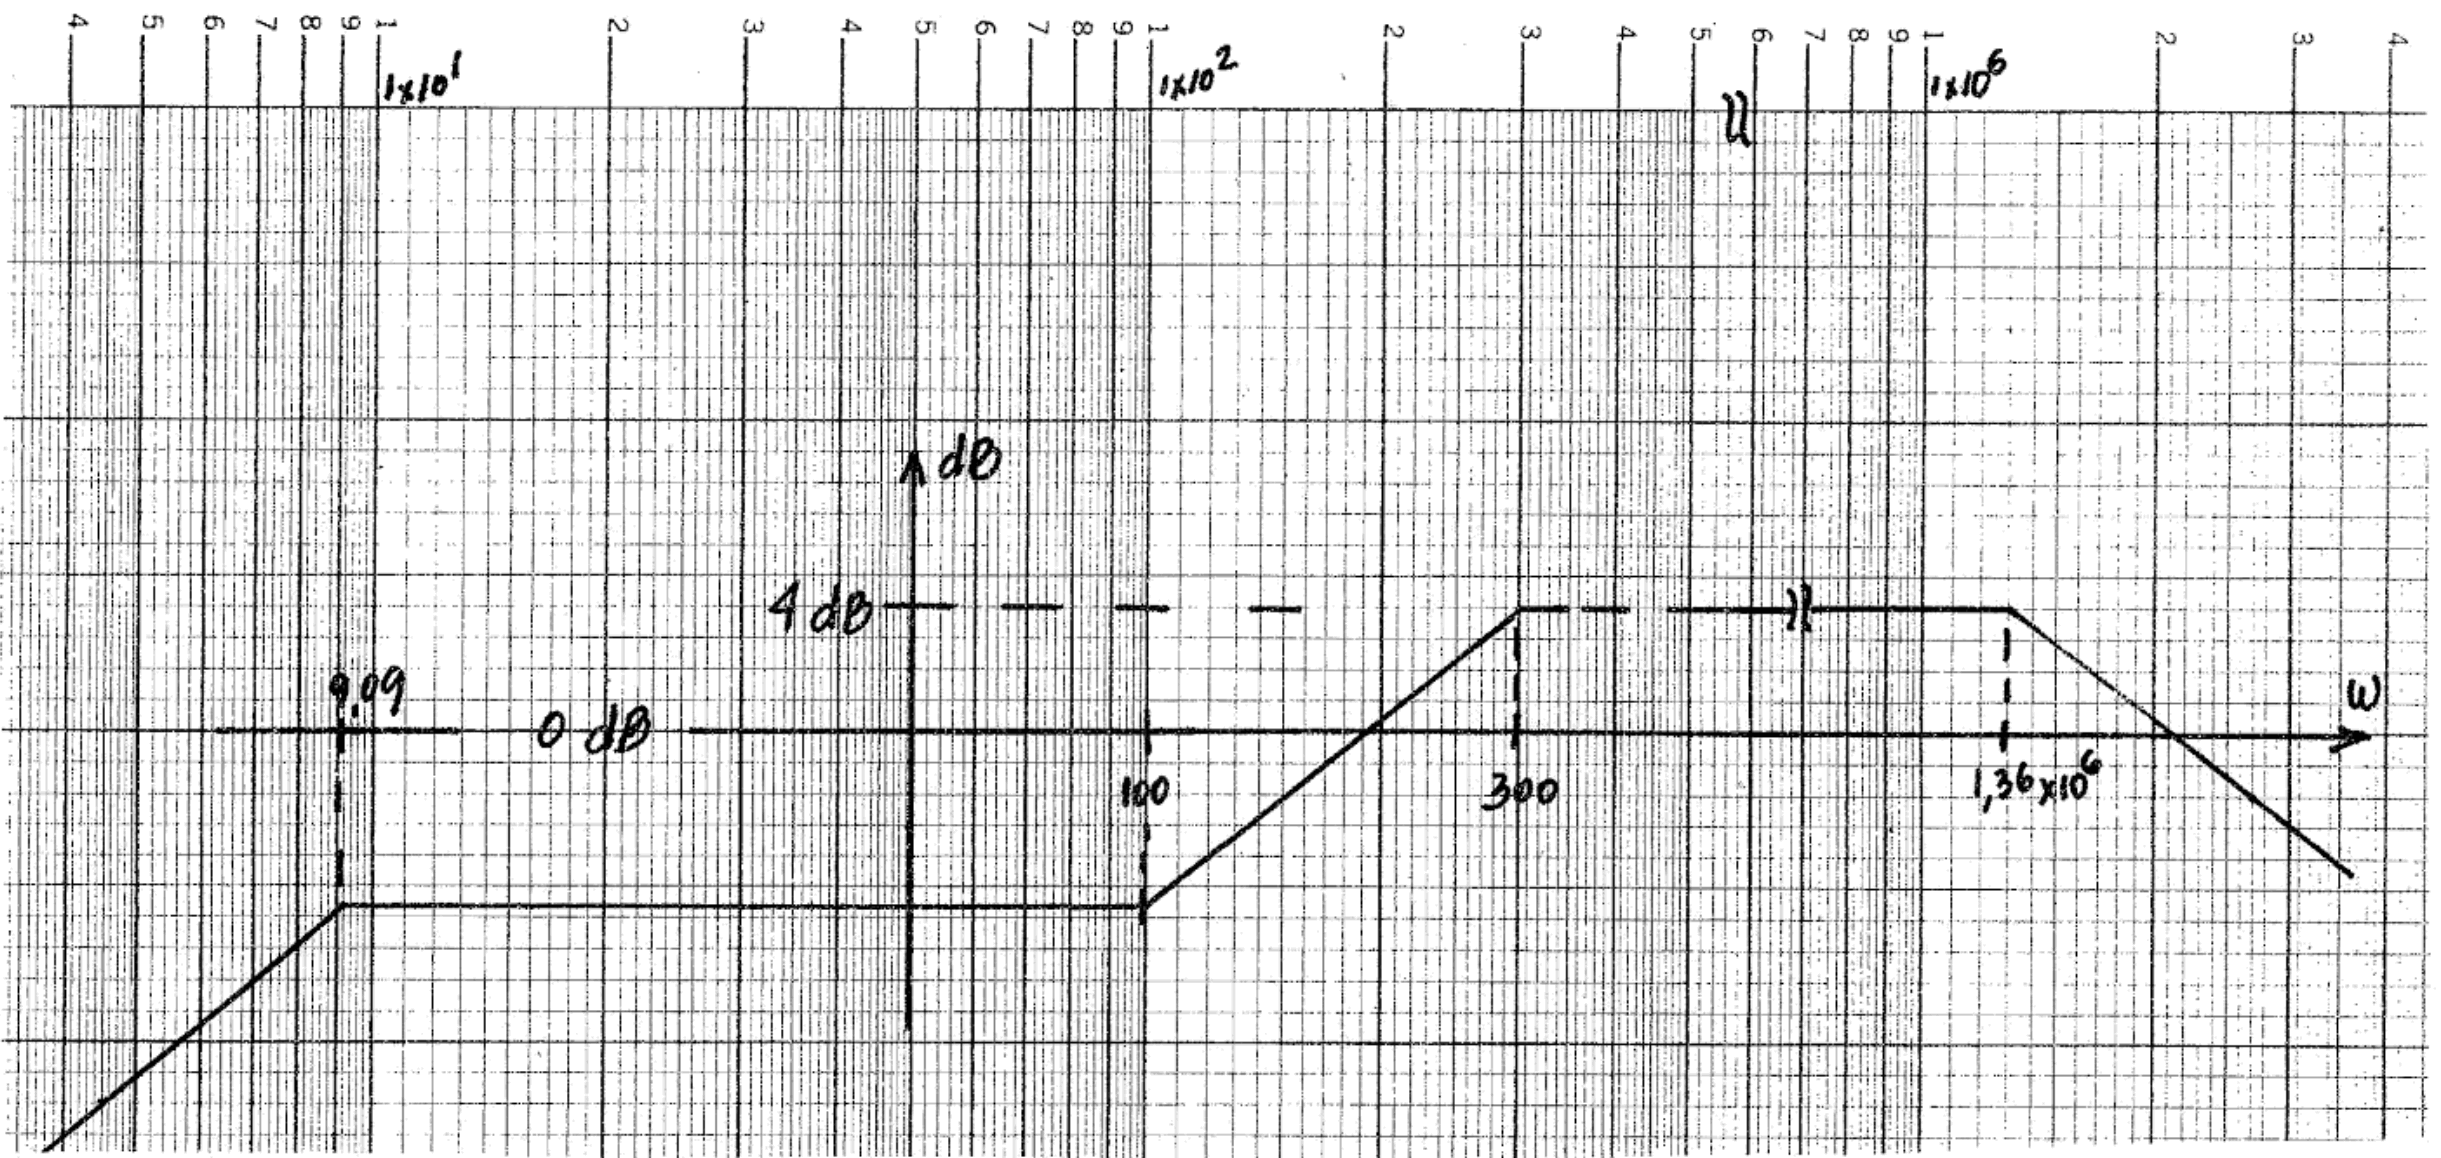
\includegraphics[width=0.9\linewidth]{_fig/respfreq_graph-ejemplo.png}
	\caption{Diagrama de Bode resultante (ejemplo)}
	\label{fig:respfreq_graph-ejemplo}
\end{figure}


\section{Método de Superposición} %p21
En la sección anterior se planteó un amplificador sencillo con FET que resultó tener una función de transferencia de cuarto orden. Se pudo simplificar el análisis en parte al despreciar el efecto de ciertos componentes según el rango de frecuencia. De ésta forma quedaban circuitos más sencillos para resolver. Sin embargo, incluso con esta simplificación, determinar la función de transferencia resultó engorroso, un problema que se agrava en circuitos más grandes. Esto representa un desafío en sistemas electrónicos complejos, compuestos frecuentemente por múltiples etapas. Programas como \textit{SPICE}, \textit{ECAP} y \textit{MICROCAP} pueden analizar redes de hasta 50 nodos, pero su enfoque numérico no identifica los componentes críticos en la función de transferencia.

Para efectos de diseño y de un análisis crudo de un circuito, lo que hace falta es un método sencillo que permita estimar las frecuencias de corte o de esquina y saber que componentes influyen en cada frecuencia de esquina. Vamos a aprovechar que conocemos la respuesta típica de un amplificador, como las que aparecen en las figuras \ref{fig:respfreq_amp-dc} y \ref{fig:respfreq_amp-dc_acomple-c}, para caracterizar simplemente con su valor de ganancia a frecuencias medias, una frecuencia de corte alta y una frecuencia de corte baja. Así se puede plantear la función de transferencia, aunque sea en forma aproximada. Por lo tanto presentamos el Método de Superposición. Con él vamos a encontrar una expresión de las raíces correspondientes a cada elemento reactivo en forma independiente. Después su efecto quedará reflejado en la frecuencia de corte baja o la frecuencia de corte alta.

El método consiste en los siguientes pasos. En primer lugar, clasificar los elementos reactivos (capacitancias e inductancias) según formen parte de \( F_L(s) \) o \( F_H(s) \):

\begin{itemize}
	\item Si el elemento actúa como filtro paso alto, pertenece a \( F_L(s) \) (elemento de \textit{baja frecuencia}).
	\item Si actúa como filtro paso bajo, pertenece a \( F_H(s) \) (elemento de \textit{alta frecuencia}).
\end{itemize}

Por ejemplo, los condensadores de acople y puenteo son de baja frecuencia, mientras las capacitancias internas del dispositivo son de alta frecuencia.

\subsection{Procedimiento para frecuencias bajas}

Se trabaja con el circuito de frecuencias bajas (condensadores de alta frecuencia como circuitos abiertos) para hallar la frecuencia de corte baja global:

\begin{enumerate}
	\item[\textbf{a)}] Cortocircuitar todos los condensadores excepto uno, \( C_K \). Calcular:
	\begin{itemize}
		\item Polo asociado:
		\begin{equation}
			\omega_{PK} = \frac{1}{R_R C_K}
		\end{equation}
		donde \( R_R \) es la resistencia de Thevenin vista desde \( C_K \).
		\item Cero asociado:
		\begin{equation}
			\omega_{ZK} = \frac{1}{R_R C_K}
		\end{equation}
		donde \( R_R \) es la resistencia en paralelo con \( C_K \).
	\end{itemize}
	
	\item[\textbf{b)}] Repetir el paso (a) para los demás condensadores de baja frecuencia.
	
	\item[\textbf{c)}] La función \( F_L(s) \) aproximada es:
	\begin{equation}
		F_L(s) = \frac{(s + \omega_{Z1})(s + \omega_{Z2}) \cdots (s + \omega_{Zm})}{(s + \omega_{P1})(s + \omega_{P2}) \cdots (s + \omega_{Pm})}
	\end{equation}
	y la frecuencia de corte baja global (\( \omega_L \)) se obtiene como:
	\[
	\omega_L = \sum_{k=1}^{m} \omega_{Pk}
	\]
\end{enumerate}

\subsection{Procedimiento para frecuencias altas}

Se analiza el circuito de frecuencias altas (condensadores de baja frecuencia como cortocircuitos):

\begin{enumerate}
	\item[\textbf{a)}] Dejar abiertos todos los condensadores excepto uno, \( C_k \). Calcular su polo asociado:
	\begin{equation}
		\omega_{Pk} = \frac{1}{R_k C_k}
	\end{equation}
	donde \( R_k \) es la resistencia de Thévenin vista desde \( C_k \). El cero se supone en \( \omega \to \infty \).
	
	\item[\textbf{b)}] Repetir el paso (a) para los demás condensadores de alta frecuencia.
	
	\item[\textbf{c)}] La función \( F_H(s) \) aproximada es:
	\begin{equation}
		F_H(s) = \frac{1}{\left(1 + \sum_{i=1}^n \frac{s}{\omega_{Pi}}\right)\left(1 + \sum_{j=1}^n \frac{s}{\omega_{Pj}}\right)\left(1 + \sum_{k=1}^n \frac{s}{\omega_{Pk}}\right)}
	\end{equation}
	\textit{Nota: La formulación original contiene sumatorias sin términos, posible error tipográfico.}
	
	La frecuencia de corte alta global es:
	\begin{equation}
		\omega_H = \frac{1}{\sum_{i=1}^n \frac{1}{\omega_{Pi}}}
	\end{equation}
\end{enumerate}

\subsection{Procedimiento para frecuencias medias}

Se calcula con condensadores de baja en corto y alta en abierto:

\begin{equation}
	A(s) = A_M \frac{1}{\left(1 + \frac{\omega_L}{s}\right)} \frac{1}{\left(1 + \frac{s}{\omega_H}\right)}
\end{equation}

\subsubsection{Ejemplo 2} \label{respfreq_ejm2}
Repita el ejemplo 1.1 utilizando este procedimiento.

\textbf{Solución:}

\textbf{Análisis de Baja Frecuencia:}

Utilice el circuito de la Figura \ref{fig:respfreq_modelo-fet-lf}

\begin{itemize}
	\item Para \( C_c \), \(R_p = \infty \):
	\[
	R_{Th} = 100k \Omega + 1M \Omega = 1.1M \Omega
	\]
	y la contribución a la función de transferencia:
	\[
	\frac{s}{s + \frac{1}{(0.1 \times 10^{-7}) \cdot 1.1 \times 10^6}} = \frac{s}{s + 9.09}
	\]
	
	\item Para \( C_s \), \( R_p = R_s \) :
	Se encuentra \( R_{Th} \) apoyado en la Figura \ref{fig:respfreq_sch-ejemplo2}.
	\begin{figure}[h]
		\centering
		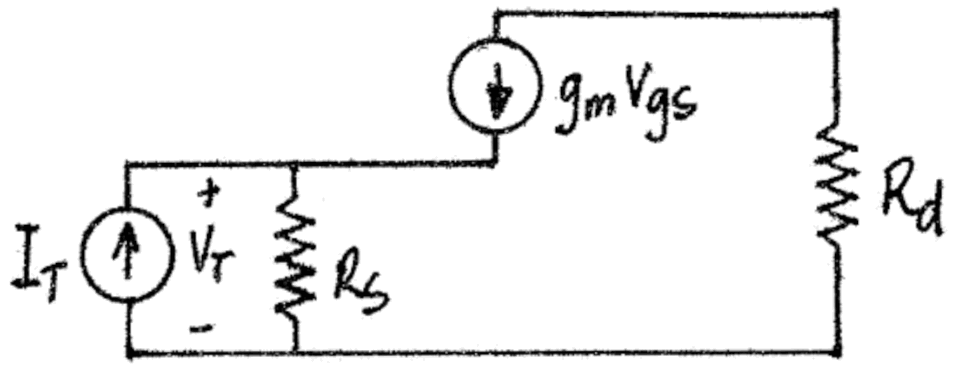
\includegraphics[width=0.9\linewidth]{_fig/respfreq_sch-ejemplo2.png}
		\caption{Circuito equivalente}
		\label{fig:respfreq_sch-ejemplo2}
	\end{figure}
	Se tiene:					
	\[
	I_T = \frac{V_T}{R_s} - g_m v_{gs}
	\]
	pero
	\[
	v_{gs} = -V_g - V_s ; V_g=0 ; V_s = V_t
	\]
	entonces
	\[
	v_{gs} = -V_T
	\]
	de donde
	\[
	I_T = V_T \left( g_m + \frac{1}{R_s} \right)
	\]
	y
	\[
	R_{Th} = \frac{V_T}{I_T} = \frac{1}{g_m + \frac{1}{R_s}} = \frac{R_s}{1 + g_m R_s}
	\]
	y su contribución a la función de transferencia:
	\[
	\frac{s + \frac{1}{C_s R_s}}{s + \frac{1 + g_m R_s}{C_s R_s}} = \frac{s + 100}{s + 300}
	\]
	y la función de transferencia de baja frecuencia queda:
	\[
	F_L(s) = \frac{s(s + 100)}{(s + 9.09)(s + 300)}
	\]
	aquí \(F_L(s)\) coincide con el resultado de \(F_L(s) \) del ejemplo 1.1. Esto no siempre se cumple y se da en éste caso por el hecho de que \( C_c \) y \( C_s \) se encuentran en mallas independientes.
\end{itemize}

\textbf{Análisis de Alta Frecuencia:}

Utilizando el circuito de la Figura \ref{fig:respfreq_relacion-vo-vi}

Para \( C_{gs} \): \( R_{Th} = 1M\Omega \parallel 100k\Omega = 90.9k\Omega \) y \( w_{cgs} = \frac{1}{90.9k \times 10^{-12}} = 1.1 \times 10^7 \)

Para \( C_{gs} \): \( R_{Th} = R_d = 2.2k \Omega \) ; la fuente \( g_m v_{gs} \) desaparece ya que la malla de entrada no llega señal, todas las tensiones en esa malla son cero, particularmente la que controla la fuente de corriente; por lo tanto la fuente de corriente es cero y se convierte en un circuito abierto.

Para \( C_{gd} \), se encuentra \( R_{Th} \) apoyado en la Figura \ref{fig:respfreq_sch-ejemplo2_c_gd}:

\begin{figure}[h]
	\centering
	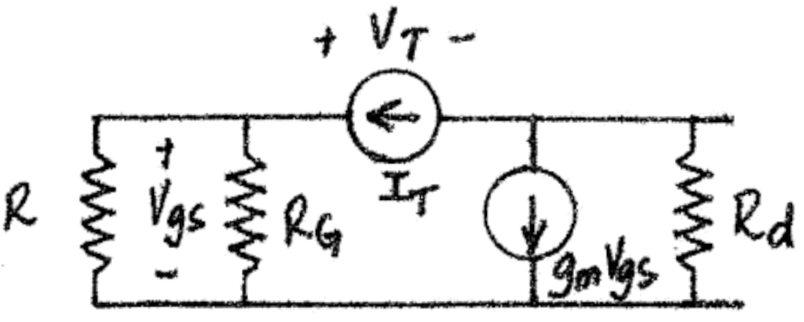
\includegraphics[width=0.9\linewidth]{_fig/respfreq_sch-ejemplo2_c_gd.png}
	\caption{ Circuito equivalente para \( C_{gd} \)}
	\label{fig:respfreq_sch-ejemplo2_c_gd}
\end{figure}

Se tiene:
\[
V_T = v_{gs} + I R_d
\]
donde \( I = g_m v_{gs} + I_T \), ademas
\[
v_{gs} = I_T (R \parallel R_G)
\]
entonces
\[
V_T = I_T \left( R \parallel R_G + g_m (R \parallel {R_g R_d}) + R_d \right)
\]
y
\[
R_h = R \parallel R_g + g_m (R \parallel { R_g R_d })  + R_d = 493k\Omega
\]
y
\[
\omega_{gd} = \frac{1}{493k\Omega 2pF} = 1.01 \times 10^6 rad/s
\]
luego
\[
\omega_H = \frac{1}{\frac{1}{1.01 \times 10^6} + \frac{1}{1.1 \times 10^7} + \frac{1}{1.52 \times 10^8}} = 923 krad/s
\]


\section{Comparación entre el método de superposición y el método exacto} %p26

Implícito en el Método de Superposición hay dos aproximaciones:

\begin{enumerate}
	\item la primera admite determinar por separado la contribución de cada elemento reactivo a la respuesta de frecuencia, cuando en realidad habrá una interacción si comparten una malla o nodo.
	\item el cálculo de las frecuencias de corte baja y alta, tal como aparecen en las ecuaciones (1.36) y (1.39).
\end{enumerate}

Generalmente el efecto de colocar en cascada a varias etapas es el de aumentar la frecuencia de corte inferior del conjunto y disminuir la frecuencia de corte superior. En la Figura 1.22 se muestra una cascada de $N$ filtros paso altos, cada uno con frecuencia de corte.

\begin{figure}[h]
	\centering
	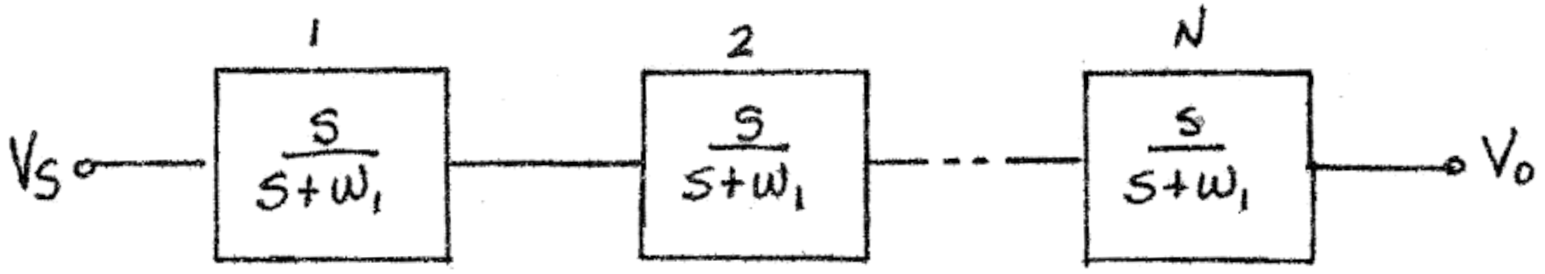
\includegraphics[width=0.9\linewidth]{_fig/respfreq_cascada-n-hp-filters.png}
	\caption{Cascada de $N$ filtros paso alto}
	\label{fig:respfreq_cascada-n-hp-filters}
\end{figure}

La función de transferencia viene dada por:

\begin{equation}
	\frac{V_o}{V_s}(s) = \frac{s^N}{(s+\omega_1)^N}
\end{equation}

Esta función tiene un valor de uno para $s$ elevada; por lo tanto, la frecuencia de media potencia, \( \omega_L \), viene dada por:

\begin{equation}
	\left| \frac{(j\omega_L)^N}{(j\omega_L + \omega_1)^N} \right| = \frac{1}{\sqrt{2}}
\end{equation}

Luego,

\[
\left[1 + \left(\frac{\omega_1}{\omega_L}\right)^2 \right]^{N/2} = 2^{1/2}
\]

\begin{equation} \label{respfreq_hp-fmp}
	\omega_L = \omega_1 \sqrt{2^{1/N} -1}
\end{equation}

Se hace notar que la raíz $N$ de $2$ da como resultado un número entre $1$ y $2$, por lo que $\omega_L$ es siempre mayor que $\omega_1$.

En forma semejante, para una cascada de $N$ filtros paso bajo con función $1/(sT_A + 1)$, la frecuencia de corte alta para la función total, $\frac{V_o}{V_s} = 1/(sT_A +1)^N$, viene dada por:

\begin{equation} \label{respfreq_hp-fc-ft}
	\omega_H = \omega_A \sqrt{2^{1/N}-1}, \quad \omega_A = \frac{1}{T_A}
\end{equation}

Es decir, la cascada de filtros de este tipo tiene el efecto de disminuir la frecuencia de corte alta. Se puede extender este análisis a un sistema filtro paso banda de banda ancha,

\[
\left(\frac{s}{s+\omega_1} \right) \left(\frac{1}{sT_A+1} \right)
\]

que se grafica en la Figura \ref{fig:respfreq_analisis-pasa-banda}.

\begin{figure}[h]
	\centering
	\subfloat[Filtro Paso Banda]
	{
		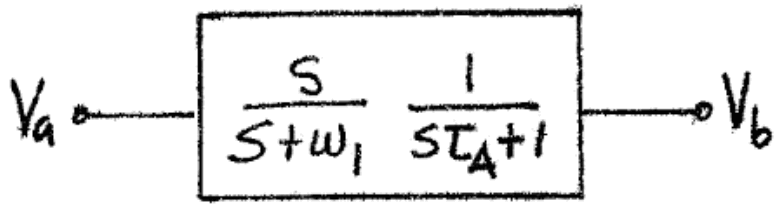
\includegraphics[width=0.4\linewidth]{_fig/respfreq_analisis-pasa-banda-filtro.png}
		\label{fig:respfreq_analisis-pasa-banda-filtro}
	}
	\subfloat[Respuesta del Módulo]
	{
		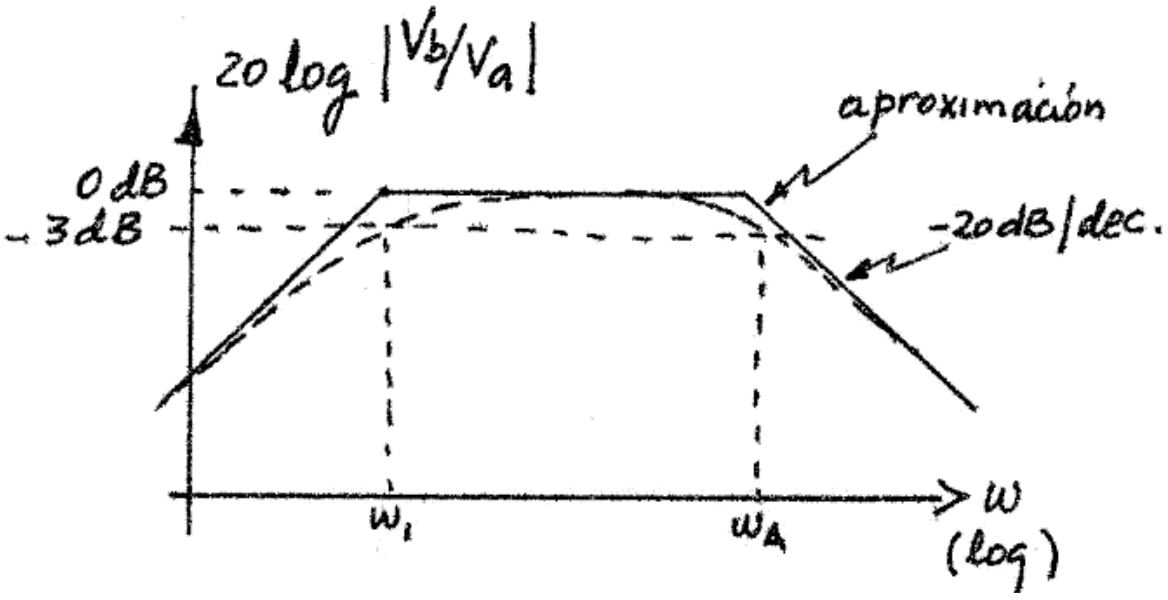
\includegraphics[width=0.4\linewidth]{_fig/respfreq_analisis-pasa-banda-resp.png}
		\label{fig:respfreq_analisis-pasa-banda-resp}
	}
	\caption{Modelo de un Amplificador Operacional con su Respuesta de Frecuencia}
	\label{fig:respfreq_analisis-pasa-banda}
\end{figure}

Al colocar dos bloques de este tipo en cascada, se consigue la función de transferencia del sistema:

\begin{equation}
	\frac{V_o}{V_s}(s) = \left[ \frac{s}{s+\omega_1} \cdot \frac{1}{sT_A+1} \right]^2
\end{equation}

La gráfica de esta función se puede trazar a partir de la Figura \ref{fig:respfreq_analisis-pasa-banda-resp}. Cada bloque tendrá esta respuesta, y el efecto de los dos es equivalente a la suma de dos de estas gráficas: el resultado se observa en la Figura \ref{fig:respfreq_analisis-pasa-banda-resp2}.

\begin{figure}[h]
	\centering
	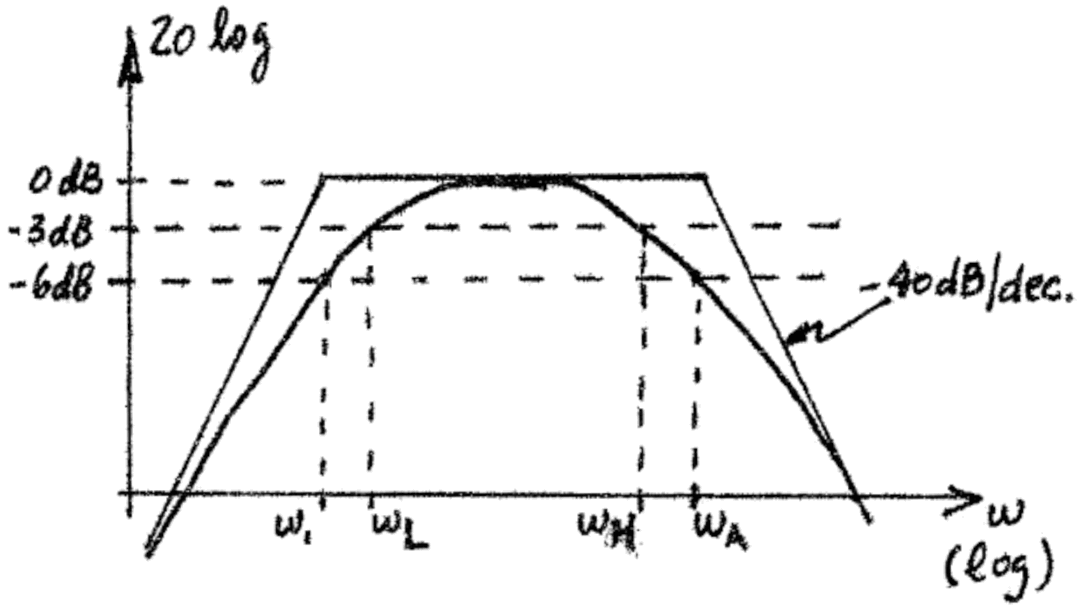
\includegraphics[width=0.8\linewidth]{_fig/respfreq_analisis-pasa-banda-resp2.png}
	\caption{Respuesta equivalente}
	\label{fig:respfreq_analisis-pasa-banda-resp2}
\end{figure}

Las asíntotas tienen valores de $+40$ dB/década por el lado de abajo debido al efecto del doble cero en el origen, y de $-40$ dB/década por el lado de arriba debido al doble polo a la frecuencia de $\omega_A$.

A las frecuencias de $\omega_1$ y $\omega_A$, la ganancia es $-6$ dB. De la curva real se puede observar que las frecuencias de media potencia, cuando la ganancia ha bajado $3$ dB, se han corrido. La frecuencia de corte baja, $\omega_L$, es mayor que la frecuencia de una etapa, $\omega_1$, y la frecuencia de corte alta, $\omega_H$, es menor que la de una etapa. El ancho de banda total es menor que el ancho de banda de una etapa.

Si los polos de alta y baja frecuencia son muy distantes, aún se cumplen las ecuaciones \ref{respfreq_hp-fmp} y \ref{respfreq_hp-fc-ft}:

\begin{itemize}
	\item Para $n=2$:
	\[
	\omega_L = \omega_1 / \sqrt{2^{1/2}-1} = 1.55\omega_1
	\]
	\[
	\omega_H = \omega_A \sqrt{2^{1/2}-1} = 0.644\omega_A
	\]
	\item Para $n=3$:
	\[
	\omega_L = \omega_1 / \sqrt{2^{1/3}-1} = 1.96\omega_1
	\]
	\[
	\omega_H = \omega_A \sqrt{2^{1/3}-1} = 0.51\omega_A
	\]
\end{itemize}

¿Qué ocurre en los casos donde las etapas no tienen las mismas frecuencias de corte? Condición que se indica en las figuras \ref{fig:respfreq_comp-metodo_ejm1-diagrama}, \ref{fig:respfreq_comp-metodo_ejm1-resp-1b2b} y \ref{fig:respfreq_comp-metodo_ejm1-resp-total}.

\begin{figure}[h]
	\centering
	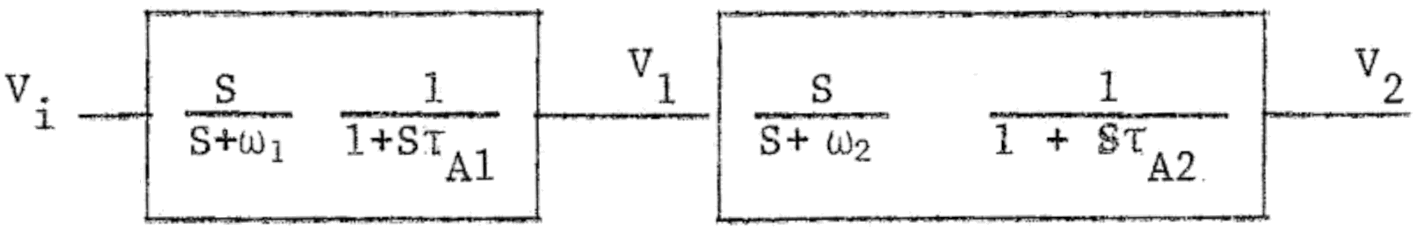
\includegraphics[width=0.9\linewidth]{_fig/respfreq_comp-metodo_ejm1-diagrama.png}
	\caption{Ejemplo: Diagrama de bloque}
	\label{fig:respfreq_comp-metodo_ejm1-diagrama}
\end{figure}

\begin{figure}[h]
	\centering
	\subfloat[Respuesta primer bloque]
	{
		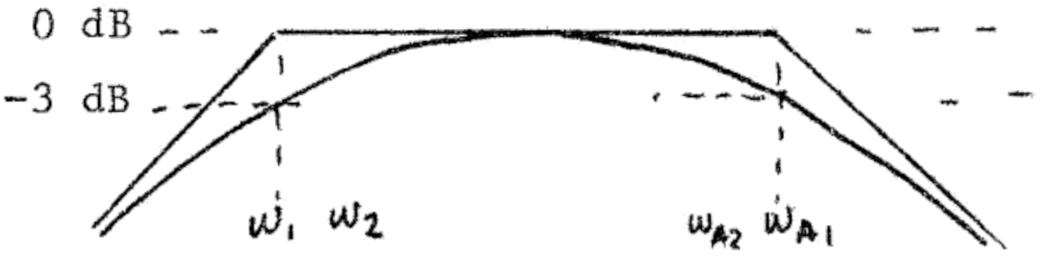
\includegraphics[width=0.4\linewidth]{_fig/respfreq_comp-metodo_ejm1-resp-1b.png}
		\label{fig:respfreq_comp-metodo_ejm1-resp-1b}
	}
	\subfloat[Respuesta segundo bloque]
	{
		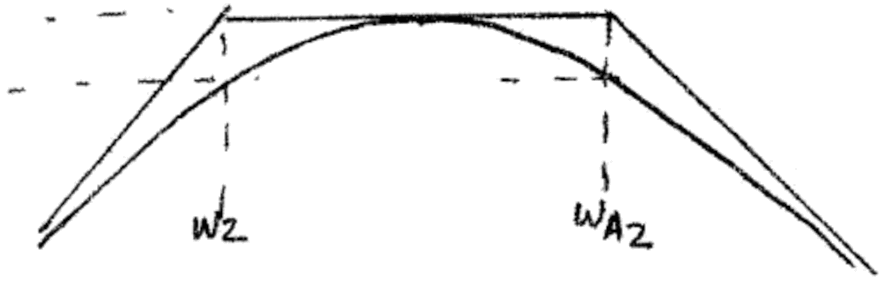
\includegraphics[width=0.4\linewidth]{_fig/respfreq_comp-metodo_ejm1-resp-2b.png}
		\label{fig:respfreq_comp-metodo_ejm1-resp-2b}
	}
	\caption{Ejemplo: Respuestas primer y segundo bloque}
	\label{fig:respfreq_comp-metodo_ejm1-resp-1b2b}
\end{figure}

\begin{figure}[h]
	\centering
	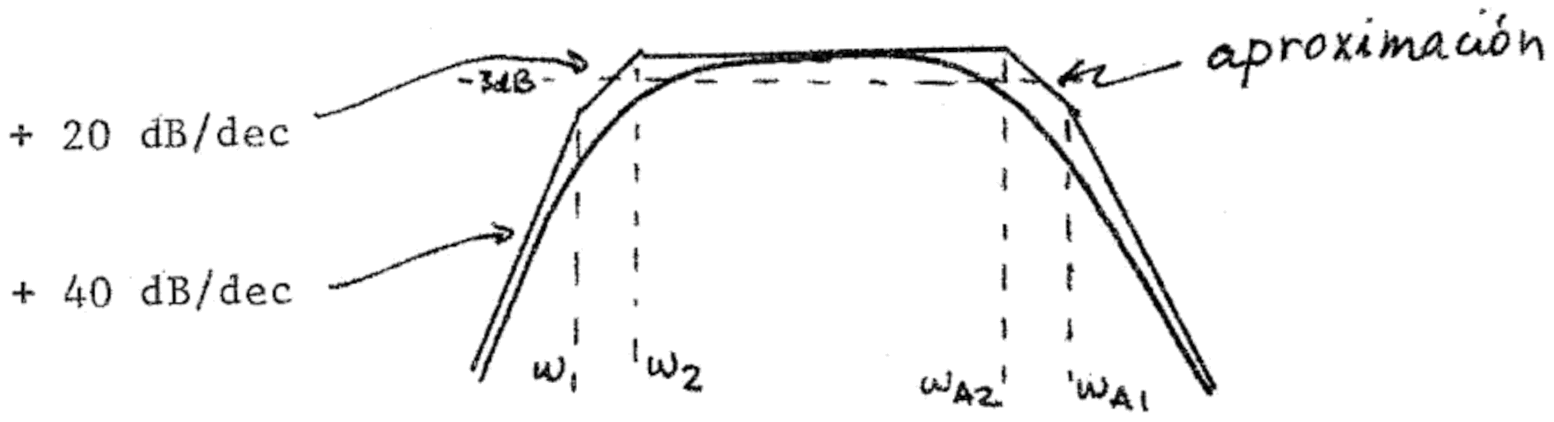
\includegraphics[width=0.9\linewidth]{_fig/respfreq_comp-metodo_ejm1-resp-total.png}
	\caption{Ejemplo: Respuesta total}
	\label{fig:respfreq_comp-metodo_ejm1-resp-total}
\end{figure}

La frecuencia de $-3$ dB tiene que ser:

\begin{description}
	\item[a.] por el lado bajo mayor que \( \omega_2 \)
	\item[b.] por el lado alto menor que \( \omega_A2 \)
\end{description}

Para los casos en que \( \omega_2 \gg \omega_1 \), entonces la frecuencia de corte inferior: \( \omega_L \approx \omega_2 \), y si \( \omega_{A2} \ll \omega_{A1} \) entonces la frecuencia de corte superior: \( \omega_H \approx \omega_{A2} \). Estos son los casos de \textbf{polo dominante}. Cuando las etapas no tienen frecuencias de corte iguales, la etapa con la frecuencia de corte más hacia el centro de la banda de paso es la que predomina en la determinación de la frecuencia de corte del conjunto.

A continuación se encuentra la expresión exacta de la frecuencia de corte superior para el caso de:

\[
G(s) = \frac{1}{(1+s/\omega_1)(1+s/\omega_2)}
\]

Por definición:

\[
G(\omega_H) = \frac{1}{\sqrt{2}} = \left| \frac{1}{1 + j\frac{\omega_H}{\left(\frac{\omega_1 + \omega_2}{2}\right)} + \frac{(j\omega_H)^2}{\omega_1\omega_2}} \right|
\]

de donde:

\begin{equation} \label{respfreq_equ-dificil}
	\omega_H^2 = -\frac{(\omega_1^2 + \omega_2^2)}{2} \pm \sqrt{\frac{(\omega_1^2 + \omega_2^2)^2}{4} + (\omega_1\omega_2)^2}
\end{equation}

\subsubsection{Ejemplo 3} \label{respfreq_ejm3}

\textbf{a)} Para \( \omega_1 = 10^6 \), \( \omega_2 = 10^6 \), se obtiene \( \omega_H = 643K \), resultado que se espera de acuerdo con la ecuación (1.44).

\textbf{b)} Para \( \omega_1 = 10^6 \), \( \omega_2 = 10^6 \), se obtiene \( \omega_H = 990K \), se hace notar la cercanía de \( \omega_H \) a \( \omega_2 \) para \( \omega_1 \gg \omega_2 \).

Es relativamente laborioso llegar a la expresión de la ecuación \ref{respfreq_equ-dificil}. Se puede imaginar lo complicado que sería determinar la expresión general de \( \omega_H \) para el caso de tres polos. Siempre se puede acudir a un computador para conseguir la solución. Sin embargo, conviene el Método de Superposición.

\section{Un enfoque distinto para graficar el diagrama de Bode del módulo} %p31

Generalmente, la función de transferencia de un amplificador se expresa como se hizo en la ecuación (1.13), que repetimos a continuación:

\[
G(s) = A_M F_L(s) F_H(s)
\]

Uno puede trazar el Diagrama de Bode del módulo sin necesidad de trazar las contribuciones individuales de las raíces. Partimos de la ganancia \( A_M \), que se convierte en nuestro punto de referencia y de allí se traza el resto del diagrama.

Por ejemplo, si 

\[
G(s) = A_M \frac{(s + \omega_1) \omega_3}{(s + \omega_2)(s + \omega_3)}
\]

\begin{equation} \label{respfreq_bodealt-eq}
	G(s) = A_M \frac{(s + \omega_1)}{(s + \omega_2)(sT_3 + 1)}
\end{equation}

donde: \( T_3 = \frac{1}{\omega_3} \); entonces \( F_L(s) = \frac{s + \omega_1}{s + \omega_2}\), \( F_H(s) = \frac{1}{sT_3 + 1}	\) y \( \omega_3 \gg \omega_2 > \omega_1 \), en la Figura \ref{fig:respfreq_bodealt} se trazan los efectos de cada una de estas componentes progresivamente hasta llegar al resultado final, la Figura \ref{fig:respfreq_bodealt-d}.

\begin{figure}[h]
	\centering
	\subfloat[A]
	{
		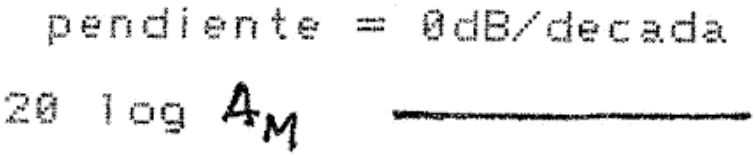
\includegraphics[width=0.2\linewidth]{_fig/respfreq_bodealt-a.png}
		\label{fig:respfreq_bodealt-a}
	}
	\subfloat[B]
	{
		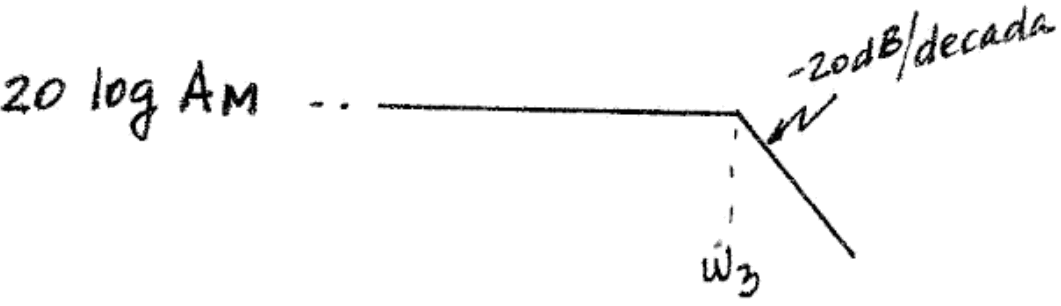
\includegraphics[width=0.32\linewidth]{_fig/respfreq_bodealt-b.png}
		\label{fig:respfreq_bodealt-b}
	}
	\subfloat[C]
	{
		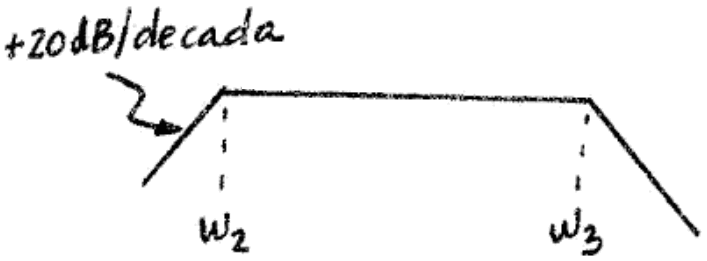
\includegraphics[width=0.2\linewidth]{_fig/respfreq_bodealt-c.png}
		\label{fig:respfreq_bodealt-c}
	}
	\subfloat[D]
	{
		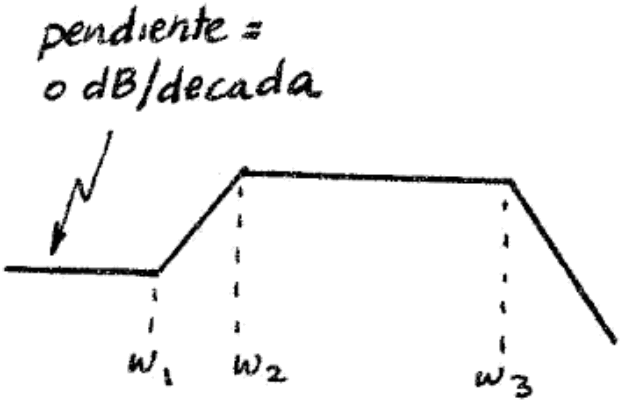
\includegraphics[width=0.2\linewidth]{_fig/respfreq_bodealt-d.png}
		\label{fig:respfreq_bodealt-d}
	}
	\caption{Ejemplo: Traza de ejemplo, Diagrama de Bode}
	\label{fig:respfreq_bodealt}
\end{figure}

Un recorrido detallado de como se analiza la Figura \ref{fig:respfreq_bodealt} es como sigue:
\begin{itemize}
	\item La ganancia a frecuencias medias es \( 20 \log A_M \), ver Figura \ref{fig:respfreq_bodealt-a}.
	\item A partir de \( \omega_3 \) comienza una pendiente de \( -20 dB/decada \) (efecto de un polo de alta frecuencia), ver Figura \ref{fig:respfreq_bodealt-b}.
	\item Desplazándonos hacia la izquierda, el polo en \( \omega_2 \) deja de contribuir su pendiente de \(-20 dB/decada \) en \( \omega_2 \), lo que resulta en una pendiente de \( +20 dB/decada \), ver Figura \ref{fig:respfreq_bodealt-c}.
	\item Desplazándonos aún más a la izquierda alcanzamos el \textbf{cero} en \( \omega_1 \); este deja de contribuir su pendiente de \( +20 dB/decada \) en \( \omega_1 \), ¡y la pendiente cambia por un valor de \( -20 dB/decada \), es decir, cambia a una pendiente de \( 0 dB/decada \), ver Figura \ref{fig:respfreq_bodealt-d}.
\end{itemize}






Funciones más complicadas se trazan utilizando el mismo enfoque.

\section{La respuesta de frecuencia de circuitos con transistores BJT} %p32

\begin{figure}[h]
	\centering
	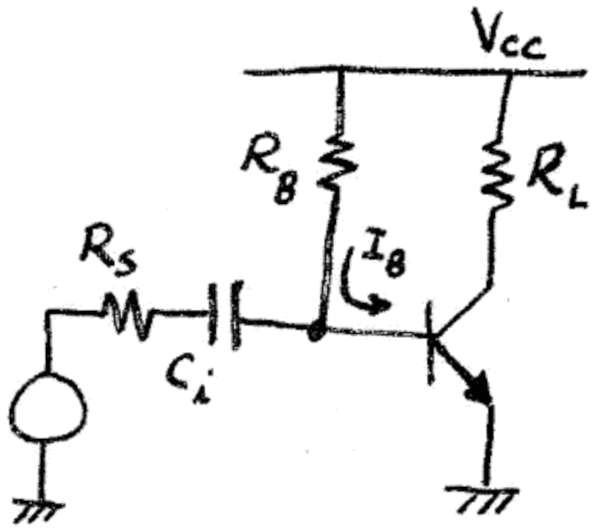
\includegraphics[width=0.35\linewidth]{_fig/respfreq_bjt-base.png}
	\caption{Amplificador emisor común}
	\label{fig:respfreq_bjt-base}
\end{figure}

Analizamos el amplificador emisor común de la Figura \ref{fig:respfreq_bjt-base}.

La resistencia \( R_B \) suministra el camino para la corriente de base de polarización. Hace falta un capacitor de acoplo \( C_i \) para desacoplar en corriente continua (c.c.) la señal de entrada de la base del transistor, evitando que se perturbe el punto de operación y permitiendo el acoplamiento en corriente alterna (c.a.).

Para corriente continua, el circuito equivalente se muestra en la Figura \ref{fig:respfreq_bjt-analisis-cc}. Este circuito se usa para determinar el punto de reposo del transistor y verificar si se encuentra en la región activa. 

Para corriente alterna, el análisis se basa en la Figura \ref{fig:respfreq_bjt-analisis-ca}, donde las fuentes de continua desaparecen: las fuentes de tensión se representan como cortocircuito y las fuentes de corriente como circuito abierto.


Y reemplazando el transistor por un modelo de la región activa, el resultado se muestra en la Figura \ref{fig:respfreq_bjt-analisis-modelo}, se presenta el modelo del transistor, el cual incluye los parámetros \( h_{fe} \) y la transconductancia \( g_m V_i \), permitiendo analizar el comportamiento del circuito en señales pequeñas.

\begin{figure}[h]
	\centering
	\subfloat[A]
	{
		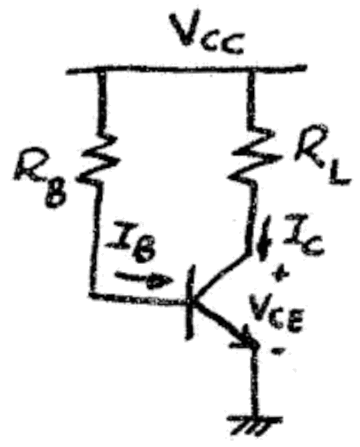
\includegraphics[width=0.15\linewidth]{_fig/respfreq_bjt-analisis-cc.png}
		\label{fig:respfreq_bjt-analisis-cc}
	}
	\subfloat[B]
	{
		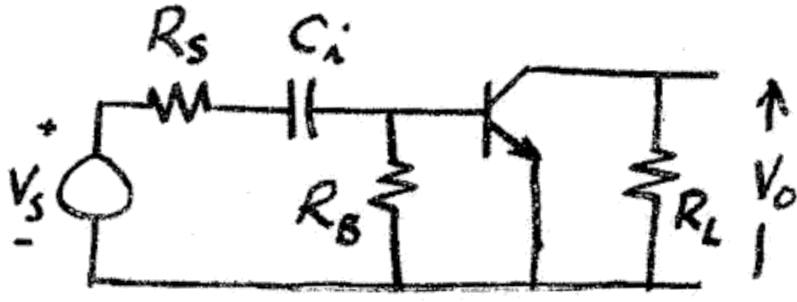
\includegraphics[width=0.25\linewidth]{_fig/respfreq_bjt-analisis-ca.png}
		\label{fig:respfreq_bjt-analisis-ca}
	}
	\subfloat[C]
	{
		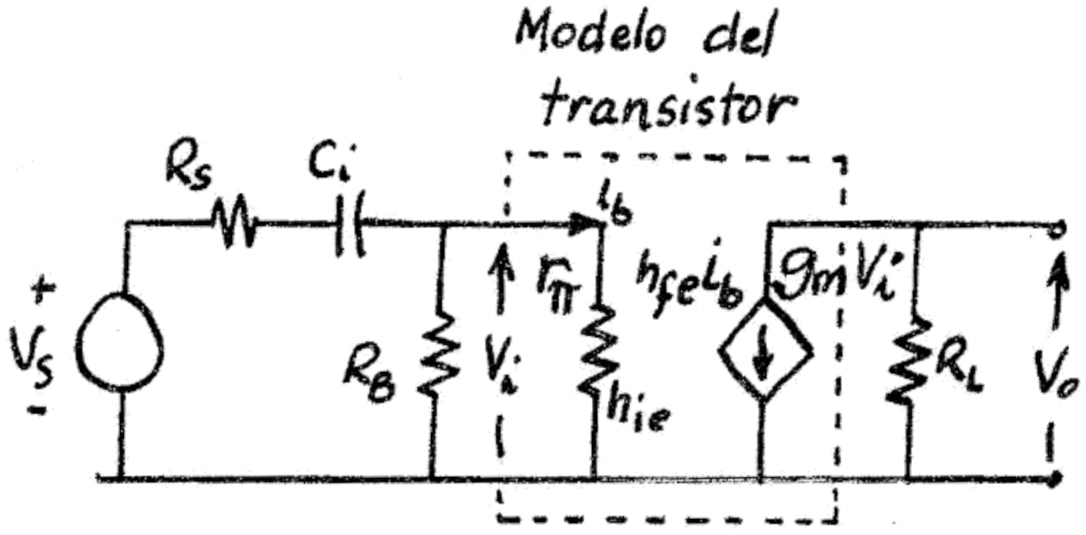
\includegraphics[width=0.5\linewidth]{_fig/respfreq_bjt-analisis-modelo.png}
		\label{fig:respfreq_bjt-analisis-modelo}
	}
	\caption{Analizando amplificador emisor común}
	\label{fig:respfreq_bjt-analisis}
\end{figure}

A frecuencias medias, la reactancia del condensador se hace despreciable y el circuito queda como se muestra en la Figura \ref{fig:respfreq_bjt-frecuencias-medias}.

\begin{figure}[h]
	\centering
	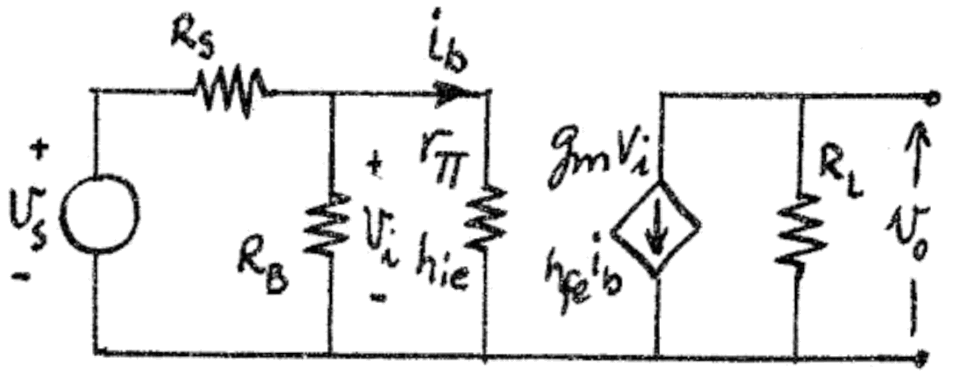
\includegraphics[width=0.6\linewidth]{_fig/respfreq_bjt-frecuencias-medias.png}
	\caption{Modelo del transistor a frecuencias medias}
	\label{fig:respfreq_bjt-frecuencias-medias}
\end{figure}

Con este circuito se obtienen los valores a frecuencias medias de la ganancia de voltaje \( A_V \), de corriente \( A_I \), la resistencia de entrada \( R_i \) y de salida \( R_o \):

\[
V_o = - g_m V_i R_L
\]

\[
V_i = \frac{R_B \parallel r_{\pi}}{R_B \parallel r_{\pi} + R_S} V_S
\]

Por lo que la ganancia de voltaje es:

\begin{equation}
	\frac{V_o}{V_S} = \frac{- g_m R_L (R_B \parallel r_{\pi})}{R_B \parallel r_{\pi} + R_S}
\end{equation}

Para conseguir la función de transferencia \( \frac{V_o}{V_S}(s) \), volvemos a la Figura \ref{fig:respfreq_bjt-analisis-modelo} consideramos que:

\begin{equation}
	\frac{V_i}{V_S} = \frac{R_B \parallel r_{\pi}}{R_B \parallel r_{\pi} + \frac{1}{C_i s} + R_S} = \frac{R_B \parallel r_{\pi}}{R_B \parallel r_{\pi} R_S} \frac{s}{s + \frac{1}{C_i (R_S + R_B \parallel r_{\pi})}}
\end{equation}

Luego:

\begin{equation} \label{respfreq_bjt-ft}
	\frac{V_o}{V_S} = \frac{- g_m R_L (R_B \parallel r_{\pi})}{R_B \parallel r_{\pi} + R_S} \frac{s}{s + \frac{1}{C_i (R_S + R_B \parallel r_{\pi})}}
\end{equation}

Esto muestra la presencia de un cero y un polo en la función de transferencia, afectando la respuesta en frecuencia del circuito.

La función está expresada en la forma de la Ecuación \ref{respfreq_bodealt-eq}. Se grafica la respuesta de frecuencia en la Figura \ref{fig:respfreq_bjt-respfreq}. Se hace notar que el: \( polo = -\frac{1}{C_i (R_S + R_B \parallel r_{\pi})} = -\frac{1}{C_i R_T}	\) donde \( R_T \) es la resistencia de Thevenin vista desde los bornes de \( C_i \).

\begin{figure}[h]
	\centering
	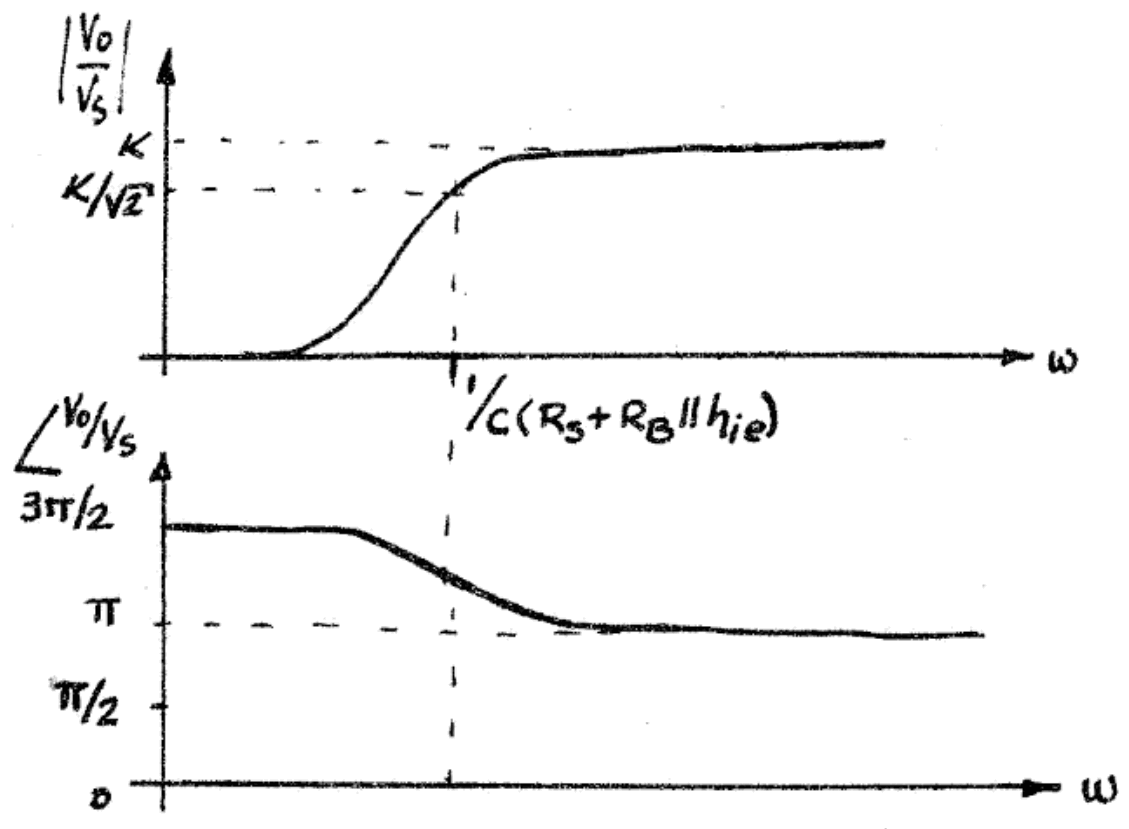
\includegraphics[width=0.6\linewidth]{_fig/respfreq_bjt-respfreq.png}
	\caption{Respuesta de frecuencia del circuito de la Figura \ref{fig:respfreq_bjt-base}}
	\label{fig:respfreq_bjt-respfreq}
\end{figure}

Dado el circuito de la Figura 1.27, los valores de \( r_{\pi} \) y \( \beta \) se encuentran en función del punto de operación sobre las características de entrada y salida del transistor, como se muestra en la Figura \ref{fig:respfreq_bjt-inout}.

\begin{figure}[h]
	\centering
	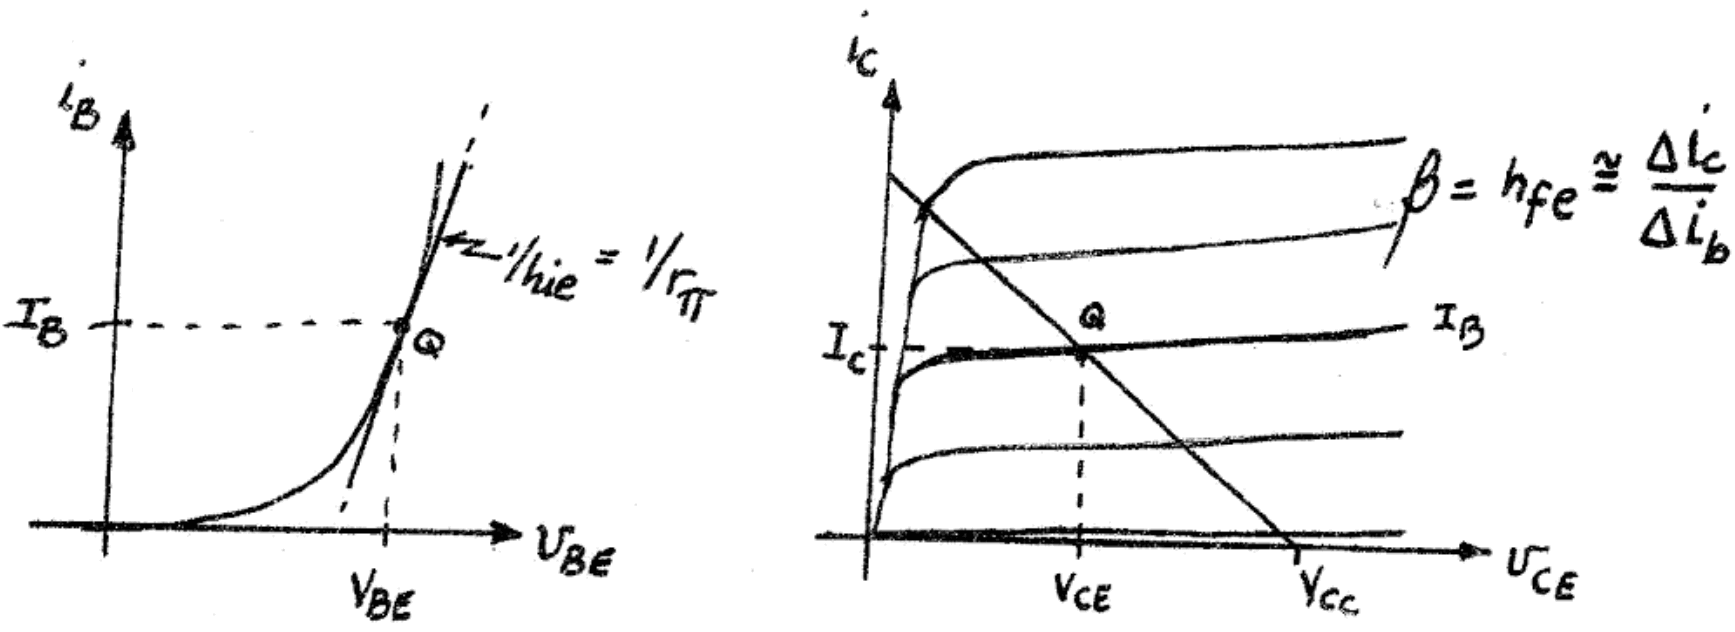
\includegraphics[width=0.6\linewidth]{_fig/respfreq_bjt-inout.png}
	\caption{Características de entrada y salida del transistor}
	\label{fig:respfreq_bjt-inout}
\end{figure}

En el circuito de la Figura \ref{fig:respfreq_bjt-con-cap-a}, se acopla una carga \( R_C \) capacitivamente al colector del transistor del circuito de la Figura \ref{fig:respfreq_bjt-base}. El cambio de la recta de carga se muestra en la Figura \ref{fig:respfreq_bjt-rectas-de-carga}.

\begin{figure}[h]
	\centering
	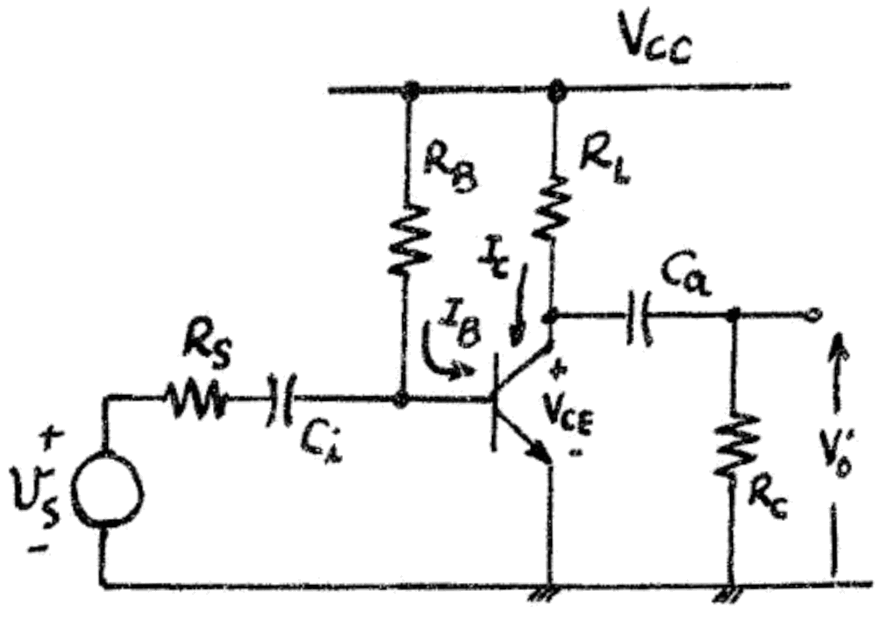
\includegraphics[width=0.5\linewidth]{_fig/respfreq_bjt-con-cap-a.png}
	\caption{Circuito con capacitancia \( C_a \)}
	\label{fig:respfreq_bjt-con-cap-a}
\end{figure}

\begin{figure}[h]
	\centering
	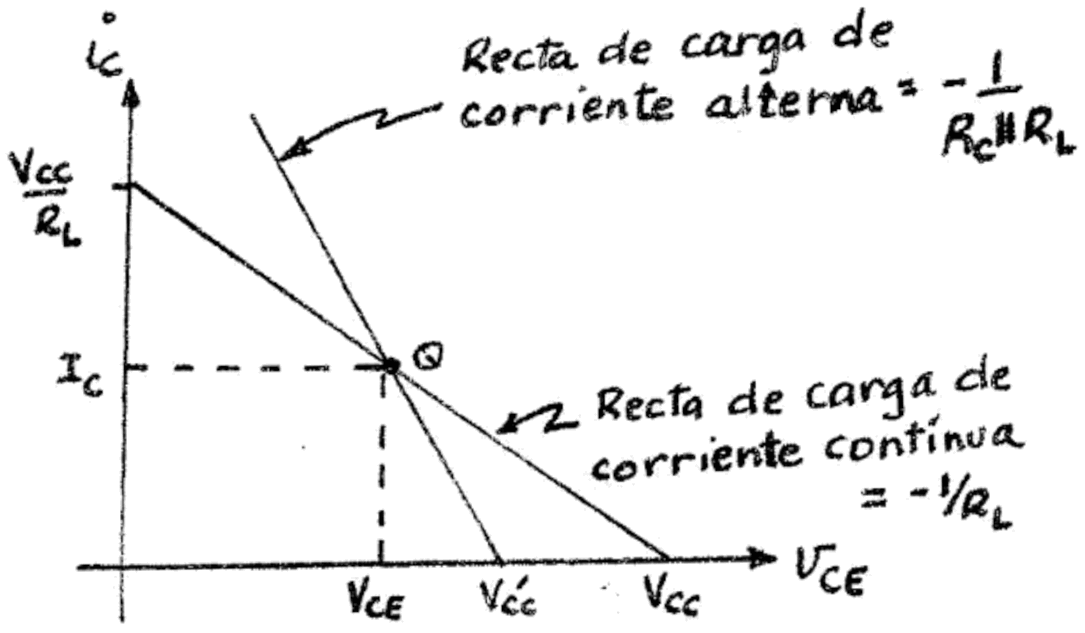
\includegraphics[width=0.6\linewidth]{_fig/respfreq_bjt-rectas-de-carga.png}
	\caption{Rectas de carga de c.a. y c.a. del circuito de la Figura \ref{fig:respfreq_modelo-fet-lf}}
	\label{fig:respfreq_bjt-rectas-de-carga}
\end{figure}

Para hallar la relación de \( \frac{V_o}{V_s} \), apenas hace falta hallar la relación \( \frac{V_o}{V_i}(s) \), pues ya encontramos la relación \( \frac{V_i}{V_s} \).

\subsection{Red de Salida para Corriente Alterna}

El circuito correspondiente se plantea en la Figura \ref{fig:respfreq_bjt-red-salida-ca}.

\begin{figure}[h]
	\centering
	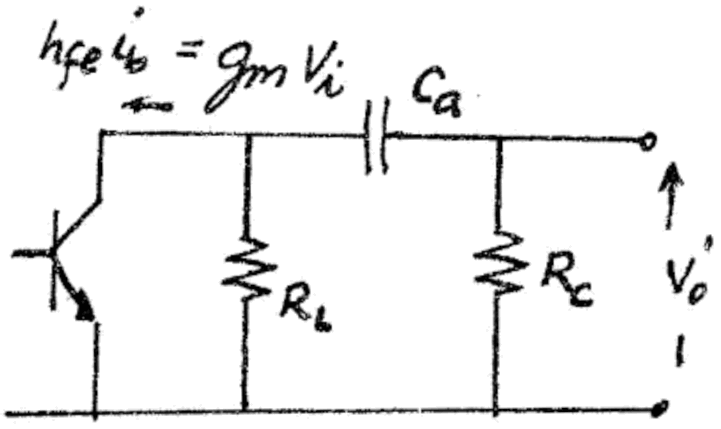
\includegraphics[width=0.5\linewidth]{_fig/respfreq_bjt-red-salida-ca.png}
	\caption{Red de salida para corriente alterna}
	\label{fig:respfreq_bjt-red-salida-ca}
\end{figure}

Reemplazando el transistor por su modelo y transformando la combinación de la fuente de corriente y \( R_L \) en su equivalente de Thevenin, nos queda la Figura \ref{fig:respfreq_bjt-eq-thevenin}.

\begin{figure}[h]
	\centering
	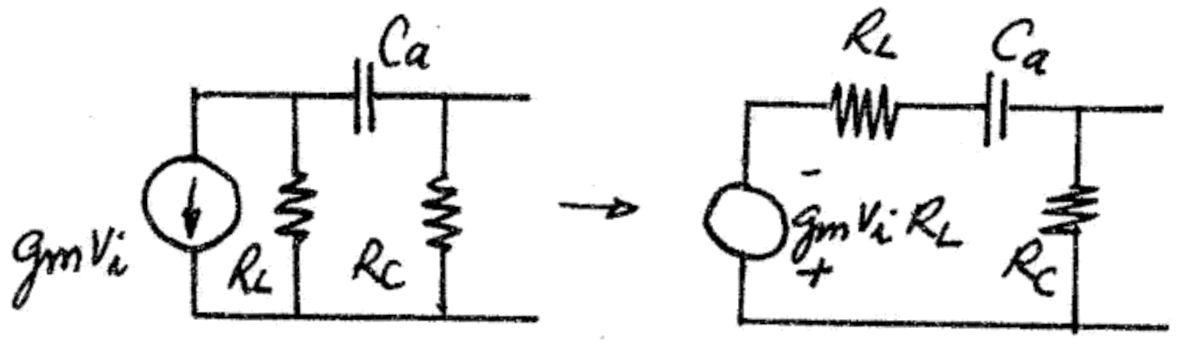
\includegraphics[width=0.6\linewidth]{_fig/respfreq_bjt-eq-thevenin.png}
	\caption{Equivalente de Thevenin}
	\label{fig:respfreq_bjt-eq-thevenin}
\end{figure}

De la Figura \ref{fig:respfreq_bjt-eq-thevenin} tenemos:

\[
V_o' = \left(\frac{-g_m V_i R_L}{R_L + R_C + \frac{1}{sC_a}}\right) R_C
\]

ó

\[
\frac{V_o'}{V_i} = -g_m R_C \parallel R_L \frac{s}{s + \frac{1}{C_a (R_C + R_L)}}
\]

Por lo tanto, dada la relación de \(V_i/V_s\) ya encontrada, tenemos:

\begin{equation} \label{respfreq_bjt-ft-analisis}
	\frac{V_o'}{V_s} = \left(-g_m R_L \parallel R_C \right) \frac{R_B \parallel r_{\pi}}{R_B \parallel r_{\pi} + R_S} \frac{s}{\left(s + \frac{1}{C_i(R_S + R_B \parallel r_{\pi})}\right)\left(s + \frac{1}{C_a(R_C + R_L)}\right)}
\end{equation}

En una comparación entre las funciones dadas en las ecuaciones \ref{respfreq_bjt-ft-analisis} y \ref{respfreq_bjt-ft}, se puede observar que la ganancia a frecuencias medias ha disminuido por el factor: \( \frac{R_L \parallel R_C}{R_L} \) debido al efecto de carga de \(R_C\).

\subsection{Caso del Condensador \( C_a \)}

El condensador \(C_a\) ha creado una pareja de cero y polo; el cero se ubica en el origen, es decir, también impide el paso de corriente continua a la salida. El polo viene dado por:

\[
-\frac{1}{C_a (R_C + R_L)} = -\frac{1}{C_a R_T}
\]

donde \(R_T\) es la resistencia de Thevenin vista desde los bornes de \(C_a\).

En la Figura \ref{fig:respfreq_bjt-bode}, se traza el Diagrama de Bode aproximado de la Ecuación \ref{respfreq_bjt-ft-analisis}, la cual tiene la forma de la Ecuación \ref{respfreq_bodealt-eq}, en donde:

\[
A_M = \frac{\left(-g_m R_L \parallel R_C \right) R_B \parallel r_{\pi}}{R_B \parallel r_{\pi} + R_S}
\]

y 

\[
F_L(s) = s / \left(s + P_{c_i} \right) \left(s + P_{c_a} \right)
\]

donde:

\[
P_{c_i} = \frac{1}{C_i(R_S + R_B \parallel r_{\pi})}
\]

\[
P_{c_a} = \frac{1}{C_a (R_C + R_L)}
\]

Al trazar la curva exacta del módulo de la función de la Ecuación \ref{respfreq_bjt-ft-analisis}, se encontrará que la frecuencia de media potencia es mayor que \( w_{B1} \).

\begin{figure}[h]
	\centering
	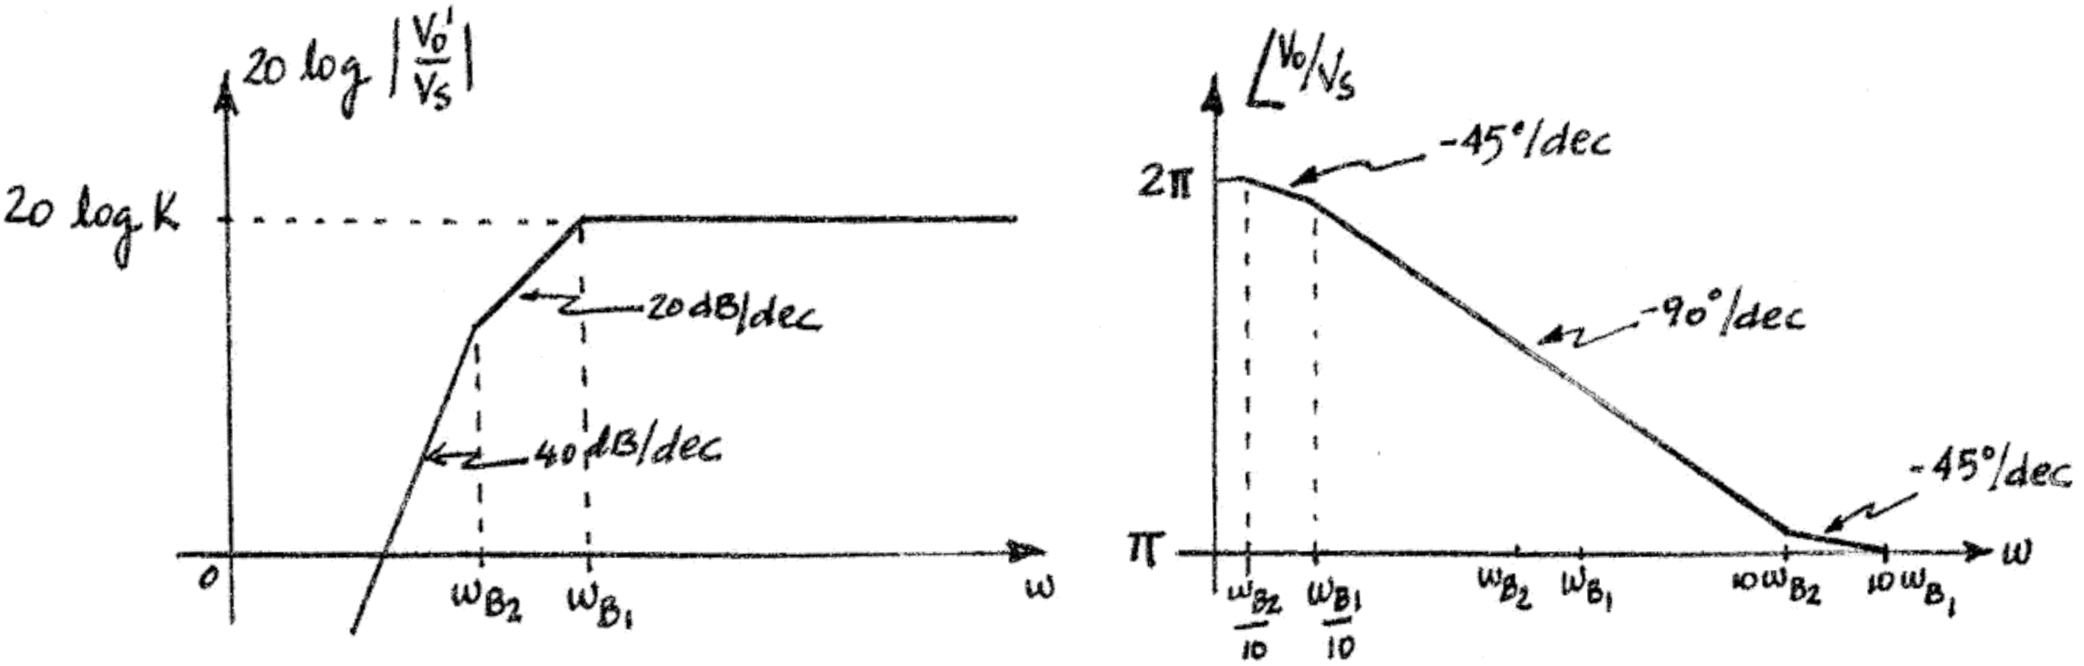
\includegraphics[width=0.9\linewidth]{_fig/respfreq_bjt-bode.png}
	\caption{Diagrama de Bode del circuito de la Fig. 1.32. Aquí se ha supuesto que los polos \( w_{B2} \) y \( w_{B1} \) debido a \( C_i \) y \( C_a \) no son iguales}
	\label{fig:respfreq_bjt-bode}
\end{figure}

\subsection{Caso del Condensador \( C_E \)}

El tercer caso que vamos a tratar es el condensador \( C_E \) que puentea la resistencia del emisor, \( R_E \), de la configuración emisor común, como se muestra en la Figura \ref{fig:respfreq_bjt-ca}, en donde se ha reemplazado la red normal de polarización por \( V_{BB} \) para simplificar el análisis del circuito.

\begin{figure}[h]
	\centering
	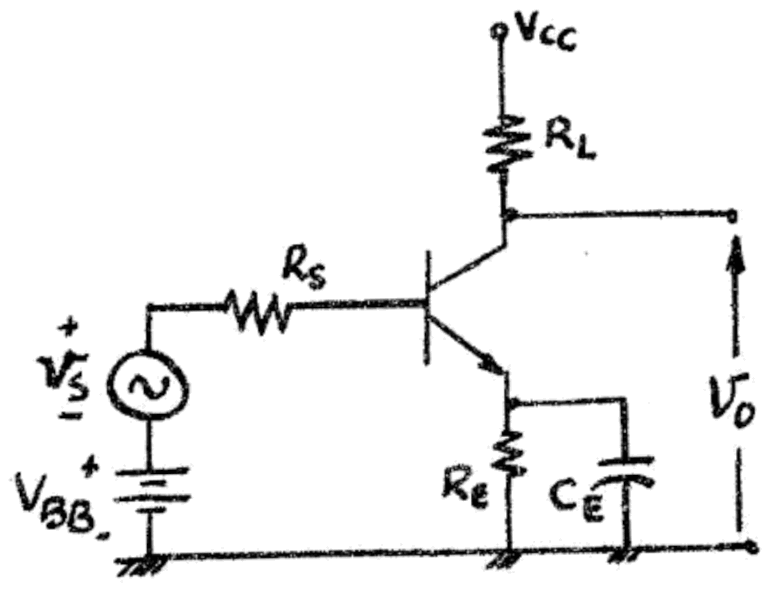
\includegraphics[width=0.5\linewidth]{_fig/respfreq_bjt-ca.png}
	\caption{Circuito BJT en corriente alterna}
	\label{fig:respfreq_bjt-ca}
\end{figure}			

En la Figura \ref{fig:respfreq_bjt-ca2} se ve el mismo circuito para corriente alterna (c.a.), donde el paralelo de \( R_E \) con \( C_E \) se considera una sola impedancia: \( Z_E = R_E \parallel \frac{1}{sC_E} \).

\begin{figure}[h]
	\centering
	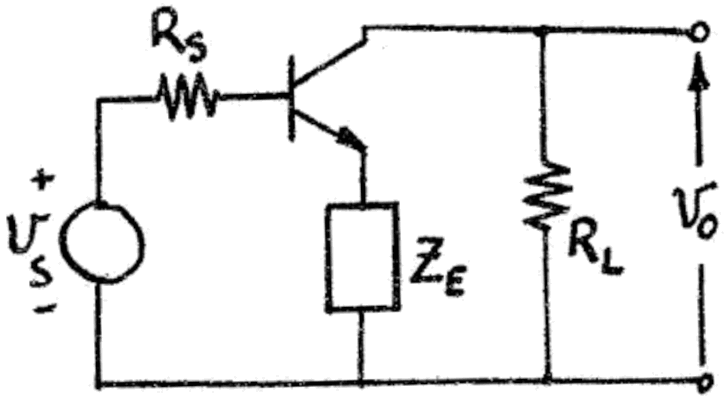
\includegraphics[width=0.5\linewidth]{_fig/respfreq_bjt-ca2.png}
	\caption{Circuito de la Figura \ref{fig:respfreq_bjt-ca} para corriente alterna}
	\label{fig:respfreq_bjt-ca2}
\end{figure}	

Este circuito tiene la misma topología de la configuración en corriente continua (E.C.) con \( R_E \), la única diferencia es que \( R_E \) ha sido reemplazado por \( Z_E \). Por lo tanto, la expresión para la ganancia \( V_o / V_s \) debe ser la misma excepto por esa diferencia.

\begin{equation}
	\frac{V_o}{V_s} = \frac{-\beta R_L}{R_s + r_{\pi} + (\beta+1)Z_E}
\end{equation}

Ahora llevaremos esta función a la forma de la ecuación \ref{respfreq_bodealt-eq}:

\[
\frac{V_o}{V_s} = \frac{-\beta R_L}{R_s + r_{\pi} + \frac{(\beta+1)R_E}{1 + R_E S C_E}}
\]

\[
\frac{V_o}{V_s} = \frac{-\beta R_L (1 + R_{E} S C_E)}{R_s + r_{\pi} + (\beta+1)R_E + R_E S C_E(R_s + r_{\pi})}
\]

\[
\frac{V_o}{V_s} = \frac{-\beta R_L R_{E} C_E (\frac{1}{R_E C_E}+S)}{R_E C_E (R_s + r_{\pi}) [\frac{R_s + r_{\pi} + (\beta+1)R_E}{R_E C_E (R_s + r_{\pi})} + S]}
\]

\begin{equation}\label{respfreq:solve2_vo-vs}
	\frac{V_o}{V_s} = \frac{-\beta R_L}{R_S + r_{\pi})} \frac{(S+\frac{1}{R_E}C_E)}{S+\frac{R_s + r_{\pi}+(\beta+1)R_E}{C_E R_E (R_s + r_{\pi})}}
\end{equation}

El circuito tiene una ganancia a frecuencias medias:

\( \frac{V_o}{V_s} (\omega \to \infty) = \frac{-\beta R_L}{R_s + r_{\pi}} \) exactamente igual a la ganancia de un circuito semejante con el emisor cortocircuitado a tierra.

El circuito tiene un cero, \( Z_1 = \frac{-1}{R_E C_E} \), y un polo, \( p_1 = \frac{R_s + r_{\pi} + (\beta+1)R_E}{C_E R_E (R_s + r_{\pi})} \)

El polo puede ser expresado de otra forma más interesante:

\[
P_1 = \frac{-(\frac{R_s+r_{\pi}}{\beta+1}+R_E)}{C_E R_E (\frac{R_s + r_\pi}{\beta+1})}			
\]

\[
P_1 =  \frac{-1}{C_E R_E \parallel (\frac{R_S+r_{\pi}}{\beta+1})}
\]

Es decir, el polo viene dado por \( -\frac{1}{C_E R_T} \), donde \( R_T \) es la resistencia de Thevenin vista desde los extremos de \(C_E\); \(R_T = R_E \parallel (\frac{R_S+r_{\pi}}{\beta+1}) \).

La expresión para esta resistencia es la misma que para la resistencia de salida de la configuración colector común; esto se debe a que en ambos casos se está viendo la resistencia entre el emisor de un transistor y tierra en paralelo con una \( R_E \) o \( R_L \).

En los tres casos que se han visto hasta ahora, los polos de los condensadores vienen dados por \( \frac{-1}{C R_T} \) donde \( R_T \) es la resistencia de Thevenin vista desde los extremos del condensador. En forma semejante, los ceros vienen dados por \( \frac{1}{C R_H} \), donde $R_H$ es la resistencia directamente en paralelo. Vea el Cuadro \ref{tab:respfreq_polos-ceros} Se hace notar que estas expresiones pueden obtenerse alternativamente por el Método de Superposición.

\begin{table}[h]
	\centering
	\begin{tabular}{|c|c|c|c|}
		\hline
		& $C_i$ & $C_a$ & $C_E$ \\ \hline
		$R_H$ & $\infty$ & $\infty$ & $R_E$ \\ \hline
		cero (z) & 0 & 0 & $\frac{1}{R_E C_E}$ \\ \hline
		$R_{TH}$ & $R_s + R_B \parallel r_{\pi}$ & $R_L + R_C$ & $R_E \parallel \frac{R_s + r_{\pi}}{\beta + 1} $ \\ \hline
		polo(p) & $\frac{-1}{C_i (R_s + R_B \parallel r_{\pi})} )$ & $ \frac{-1}{C_a (R_L + R_C)}$ & $\frac{-1}{C_E R_E \parallel \frac{R_s + r_{\pi}}{\beta+1}}$ \\ \hline
	\end{tabular}
	\caption{Polos y Ceros de los casos \(C_i\), \(C_a\), \(C_E\)}
	\label{tab:respfreq_polos-ceros}
\end{table}

\begin{figure}[h]
	\centering
	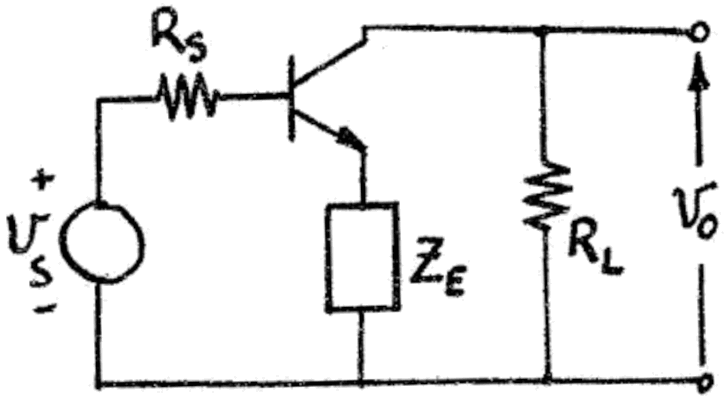
\includegraphics[width=0.5\linewidth]{_fig/respfreq_bjt-ca2.png}
	\caption{Circuito de la Figura \ref{fig:respfreq_bjt-ca} para corriente alterna}
	\label{fig:respfreq_solve2_bode}
\end{figure}	

Se traza el Diagrama de Bode aproximado de la ecuación \ref{respfreq:solve2_vo-vs} en la Figura \ref{fig:respfreq_bode_bjt_ca}. Se hace notar que necesariamente el valor del cero es menor que el valor del polo ya que:

\[
R_E > R_E \parallel \frac{R_s + r_{\pi}}{\beta + 1}
\]

\begin{figure}[h]
	\centering
	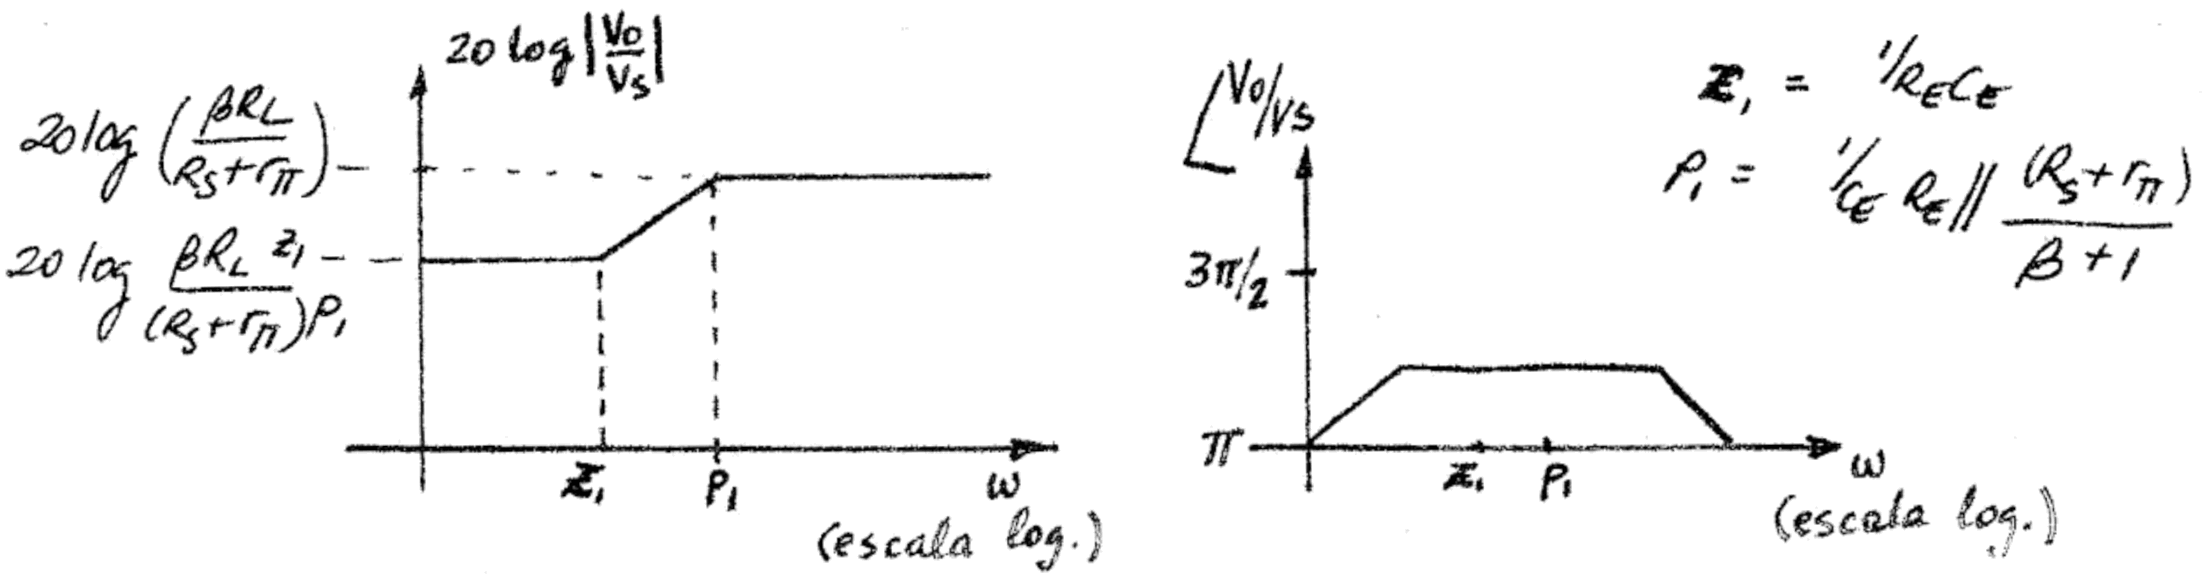
\includegraphics[width=0.8\linewidth]{_fig/respfreq_bode_bjt_ca.png}
	\caption{Diagrama de Bode de la Figura \ref{fig:respfreq_bjt-ca}}
	\label{fig:respfreq_bode_bjt_ca}
\end{figure}

El valor de la ganancia para \( \omega << z_1 \), es:

\begin{equation}
	\frac{V_o}{V_s} = \frac{-\beta R_L z_1}{(R_s + r_{\pi}) p_1} = \frac{-\beta R_L}{R_s + r_{\pi} + (\beta+1)R_E}
\end{equation}

A la vez, esta expresión la reconocemos como la ganancia de la configuración emisor común con \( R_E \); esto es lógico ya que a frecuencias suficientemente bajas, el condensador se comporta como un circuito abierto, y el circuito de la figura 1.37 queda como un E.C. con \( R_E \).

\begin{figure}[h]
	\centering
	\subfloat[Circuito Original]
	{
		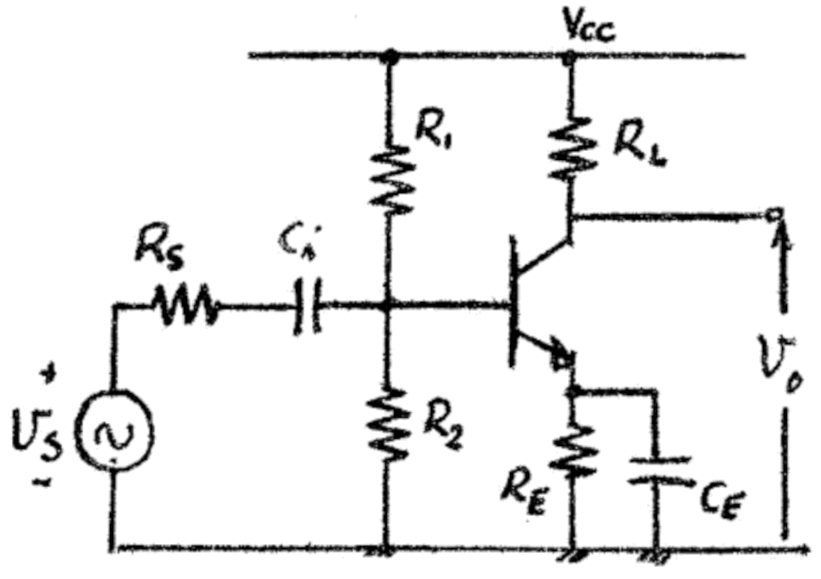
\includegraphics[width=0.44\linewidth]{_fig/respfreq_emisor-comun-autolarizado_original.png}
		\label{fig:respfreq_emisor-comun-autolarizado_original}
	}
	\subfloat[Equivalente para C.A.]
	{
		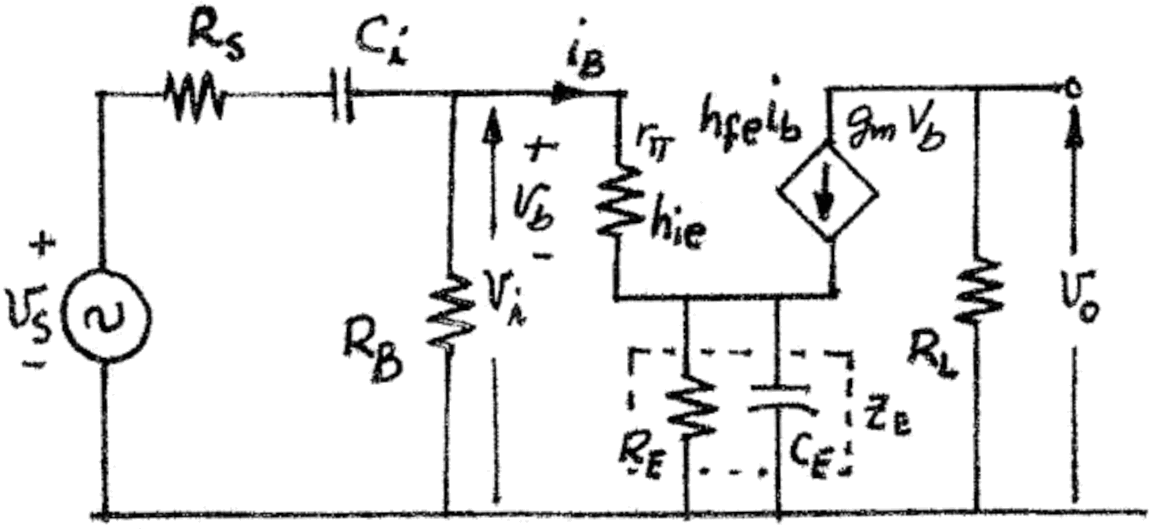
\includegraphics[width=0.44\linewidth]{_fig/respfreq_emisor-comun-a_equiv-ca.png}
		\label{fig:respfreq_emisor-comun-a_equiv-ca}
	}
	\caption{Emisor Común Autopolarizado}
	\label{fig:respfreq_emisor-comun-autolarizado}
\end{figure}

\subsubsection{Ejemplo 4} \label{respfreq_ejm4}

Determine la función de transferencia del circuito de la Figura \ref{fig:respfreq_emisor-comun-autolarizado} por el Método Exacto y el Método de Superposición.

\textbf{Solución:}

Para hallar la función de transferencia exacta, \( \frac{V_o}{V_s}(s) \), se trabaja con las ecuaciones de malla y nodo de este circuito. Así:

\[
v_o =  - \beta i_B R_L
\]

\[
i_B = \frac{V_i}{Z_i}
\]

donde \( Z_i = r_{\pi} + (\beta + 1)Z_E \), donde \( Z_E = \frac{R_E}{(1 + {s R_E C_E}} \)

y,

\[
v_i = \frac{{R_B \parallel Z_i}V_S}{{R_B \parallel  Z_i} + \frac{1}{S C_i} + R_s} = \frac{R_B Z_i S C_i V_s}{{R_B Z_i S C_i}+(R_B + Z_i)(1+ {S C_i R_s})}
\]

Uno ahora reemplaza $Z_i$ por su expresión equivalente y se trabaja con las expresiones hasta conseguir \( V_o/V_s \) de la forma:

\[
\frac{V_o}{V_s} = K \frac{s(s+\omega_1)}{s^2+bs+c}
\]

Sin embargo, al hacerlo, uno se convence rápidamente que es una labor muy engorrosa, resultando una cantidad de productos y sumas que difícilmente pueden interpretarse en relación al circuito, y además se presta para equivocaciones. ¡Como sería con 3 condensadores!

\textbf{Por el Método de Superposición:}

\begin{figure}[h]
	\centering
	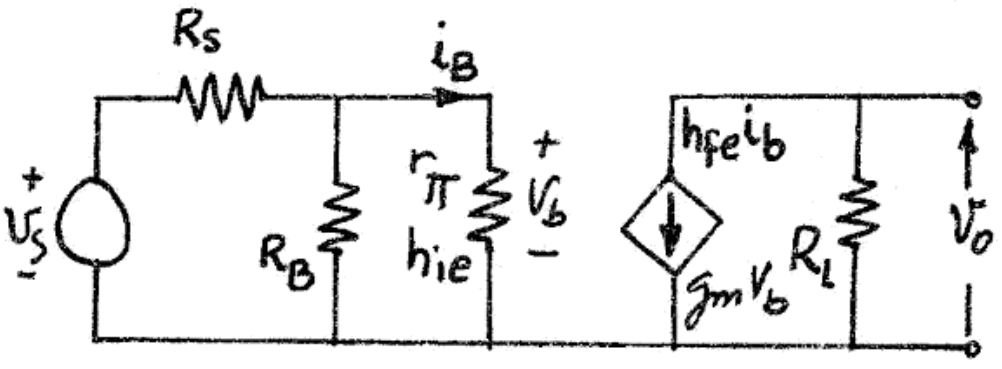
\includegraphics[width=0.8\linewidth]{_fig/respfreq_emisor-comun-autolarizado_c-short.png}
	\caption{Figura \ref{fig:respfreq_emisor-comun-autolarizado} con los C's cortocircuitados}
	\label{fig:respfreq_emisor-comun-autolarizado_c-short}
\end{figure}

\textbf{a)} El circuito a frecuencias medias, \( \omega_m \), para calcular \( A_M \) se muestra en la \ref{fig:respfreq_emisor-comun-autolarizado_c-short}, de donde se consigue:

\[
\frac{V_o}{V_s}(\omega_m) = A_M = \frac{-g_m R_L {R_{B} \parallel r_{\pi}}}{(R_s + {R_{B} \parallel r_{\pi}}}
\]

\begin{figure}[h]
	\centering
	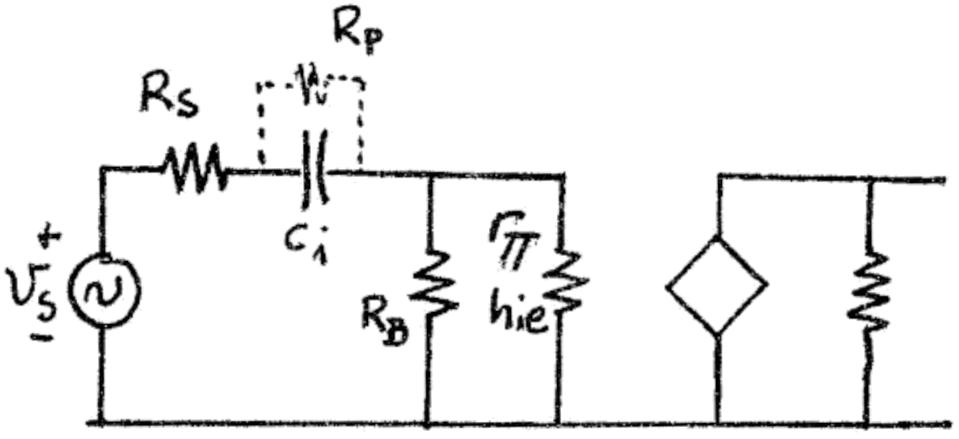
\includegraphics[width=0.8\linewidth]{_fig/respfreq_emisor-comun-autolarizado_calc_ci.png}
	\caption{Circuito apto para calcular \( \frac{s+z_{ci}}{s+p_{ci}} \)}
	\label{fig:respfreq_emisor-comun-autolarizado_calc_ci}
\end{figure}

\textbf{b)} El circuito para calcular polo y cero debido a $C_i$ se muestra en la Figura \ref{fig:respfreq_emisor-comun-autolarizado_calc_ci}.

La $R_p$ en paralelo con $C_i = \infty$.

La $R_T$ vista desde $C_i = R_s + R_{B} \parallel r_{\pi}$.

\begin{figure}[h]
	\centering
	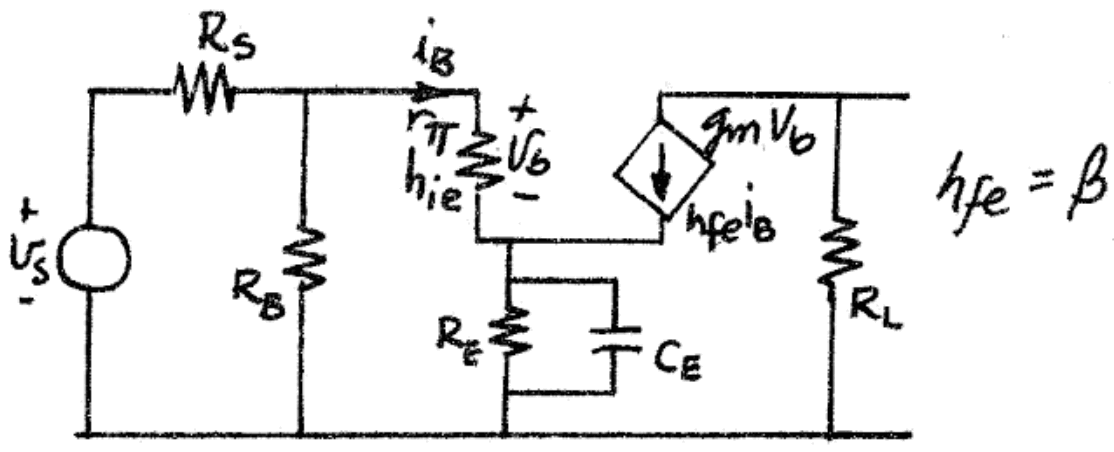
\includegraphics[width=0.8\linewidth]{_fig/respfreq_emisor-comun-autolarizado_calc_ce.png}
	\caption{Circuito apto para los polos y ceros debido a $C_E$}
	\label{fig:respfreq_emisor-comun-autolarizado_calc_ce}
\end{figure}

\textbf{c)} El circuito para calcular polo y cero debido a $C_E$ se muestra en la Figura \ref{fig:respfreq_emisor-comun-autolarizado_calc_ce}.

La $R_p = R_E$.

La $R_T = R_E \parallel \frac{R_s + R_{B} + r_{\pi}}{\beta + 1} $

\textbf{d)} En total, la función de transferencia queda:

\begin{equation}
	\frac{V_o}{V_s}(s) = \frac{-g_m R_L R_{B} \parallel r_{\pi}}{R_{B} \parallel r_{\pi} + R_s} \frac{s {s + \frac{1}{R_E C_E}}}{(s + \frac{1}{C_i (R_s + R_{B} \parallel r_{\pi})})(s + \frac{1}{C_E (R_E \parallel \frac{R_s + r_{\pi}}{\beta + 1})})}
\end{equation}

\section{Un modelo de transistor apto para altas frecuencias} %p44

Los amplificadores transistorizados, como el de la Figura \ref{fig:respfreq_bjt-base}, sufren pérdidas en su ganancia a frecuencias altas que no se preveen de acuerdo al modelo simplificado híbrido. Surge la necesidad de algo más para el estudio a altas frecuencias.

Existen dos mecanismos en el transistor cuyo efecto es capacitivo:

\begin{enumerate}
	\item Una capacitancia de difusión para la junta directamente polarizada, dependiente del nivel de corriente contínua del colector, $I_C$
	\item Dos capacitancias, una a través de cada junta, que son dependientes de la tensión a través de esas juntas, como se indica en la Figura \ref{fig:respfreq_transistor-cap-internas}.
\end{enumerate}

\begin{figure}[h]
	\centering
	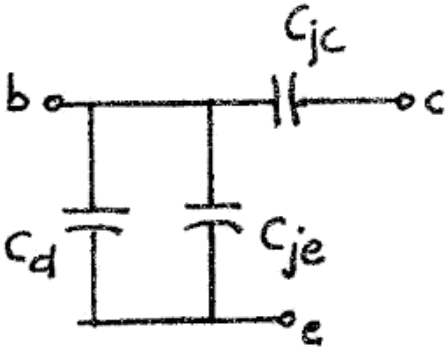
\includegraphics[width=0.5\linewidth]{_fig/respfreq_transistor-cap-internas.png}
	\caption{Capacitancias internas del transistor}
	\label{fig:respfreq_transistor-cap-internas}
\end{figure}

Hay caídas de Voltaje en la base entre los bornes externos y la región interna de operación, tal como se indica en la Figura \ref{fig:respfreq_transistor-construccion-y-regiones}. Esta se representa en el modelo por $r_b$.

\begin{figure}[h]
	\centering
	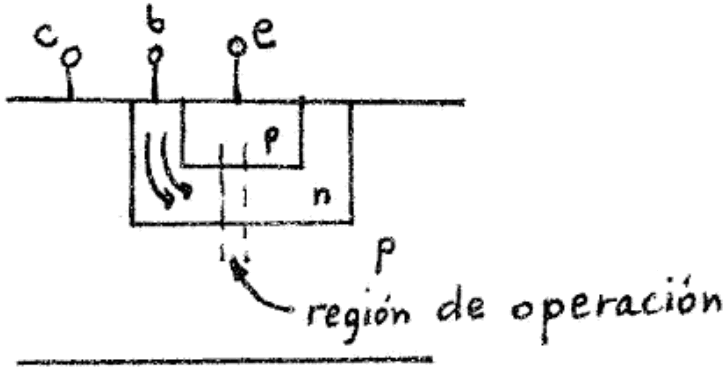
\includegraphics[width=0.5\linewidth]{_fig/respfreq_transistor-construccion-y-regiones.png}
	\caption{Construcción Física del Transistor y la Región de Operación}
	\label{fig:respfreq_transistor-construccion-y-regiones}
\end{figure}		

Se anexan las capacitancias de junta y de difusión, la resistencia $r_b$ al modelo $\pi$ híbrido simplificado para llegar al modelo $\pi$ híbrido de alta frecuencia que se muestra en la Figura \ref{fig:respfreq_transistor-modelo-hf}.

\begin{figure}[h]
	\centering
	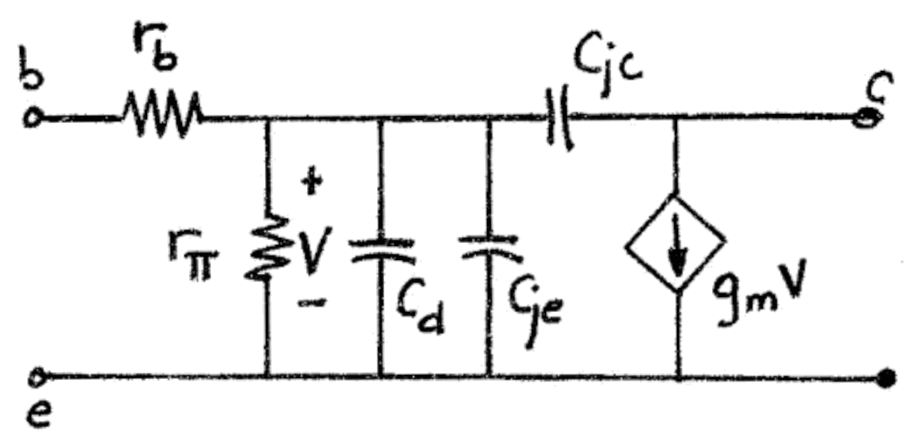
\includegraphics[width=0.6\linewidth]{_fig/respfreq_transistor-modelo-hf.png}
	\caption{Modelo híbrido de alta frecuencia}
	\label{fig:respfreq_transistor-modelo-hf}
\end{figure}

Una variación de tensión en la unión colector base produce una ligera modificación del ancho de la base, que a su vez produce un cambio en la corriente de colector. Este efecto se representa con una conductancia $g_{bc}$ entre el colector y la base interna, $b'$. Para completar el modelo se anexa una conductividad, $g_{ce}$, entre el colector y el emisor. El modelo completo se muestra en la Figura \ref{fig:respfreq_transistor-hibrido-completo}.

\begin{figure}[h]
	\centering
	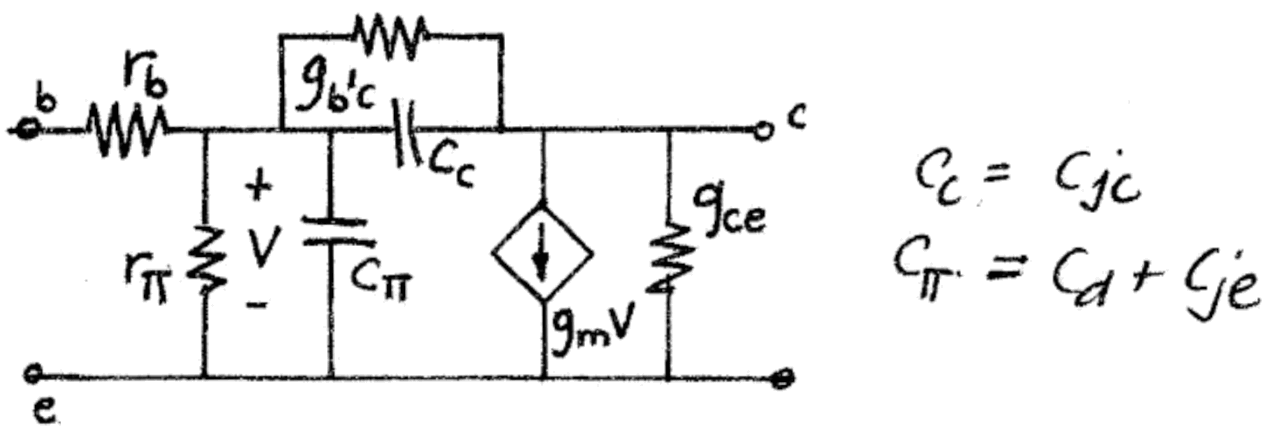
\includegraphics[width=0.5\linewidth]{_fig/respfreq_transistor-hibrido-completo.png}
	\caption{Modelo híbrido completo}
	\label{fig:respfreq_transistor-hibrido-completo}
\end{figure}

$C_c = C_{jc}$

$C_{\pi} = C_d + C_{je}$

\subsection{Comparación con el Modelo de los Parámetros $h$}

Relacionamos el modelo $\pi$ híbrido a bajas frecuencias, donde las capacitancias se desprecian en la forma de un circuito abierto, con un modelo muy conocido, el de los parámetros h, tal como se ven en la Figura \ref{fig:respfreq_model-t}.

\begin{figure}[h]
	\centering
	\subfloat[Modelo $\pi$ híbrido a bajas frecuencias]
	{
		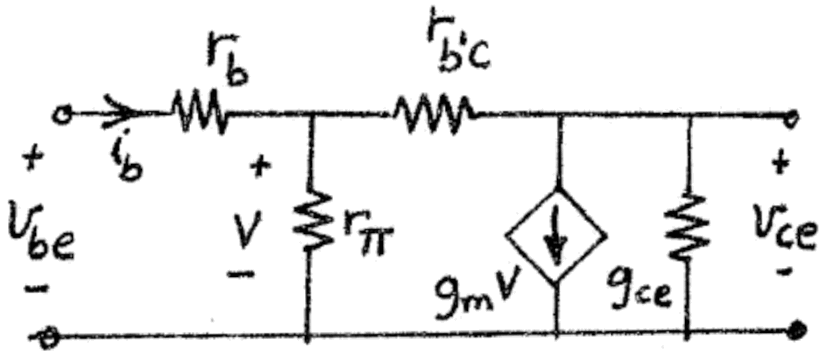
\includegraphics[width=0.44\linewidth]{_fig/respfreq_model-t_pi-hibrido.png}
		\label{fig:respfreq_model-t_pi-hibrido}
	}
	\subfloat[Modelos de los paránmetros $h$]
	{
		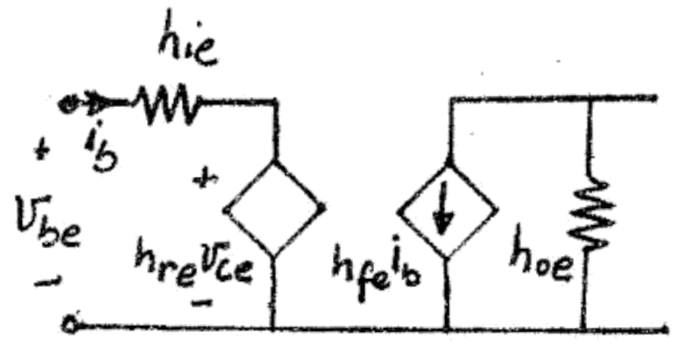
\includegraphics[width=0.44\linewidth]{_fig/respfreq_model-t_parametros-h.png}
		\label{fig:respfreq_model-t_parametros-h}
	}
	\caption{Modelos del transistor}
	\label{fig:respfreq_model-t}
\end{figure}

\begin{enumerate}
	\item La corriente de salida del circuito con la salida en corto circuito es $g_m v$ en un caso y $h_{fe} i_b$ en el otro. $h_{fe}$ es la ganancia de corriente en ortocircuito y es igual a $\beta$ del transistor.
	
	Entonces, $g_m v = h_{fe} i_b$ si suponemos que $r_{bc} \approx \infty$ da $v = i_b r_{\pi}$ y $g_m i_b r_{\pi} = h_{fe} i_b$ ó:
	
	\begin{equation}
		g_m r_{\pi} = h_{fe}
	\end{equation}
	
	\item Con la entrada abierta, $h_{re} = \frac{v}{v_{ce}}$ es la ganancia inversa de voltaje. A la vez:
	
	\begin{equation}
		\frac{v}{v_{ce}} = \frac{r_{\pi}}{r_{\pi} + r_{bc}} \to r_{bc} = \frac{r_{\pi}}{h_{re}}
	\end{equation}
	
	que se ve es un valor muy grande pues $h_{re}$ es siempre muy pequeño.
	
	\item La impedancia de entrada con la salida en cortocircuito es:
	
	\begin{equation}
		h_{ie} = r_{\pi} + r_b
	\end{equation}
	
	\item Con la entrada en circuito abierto se consigue $h_{oe}$, la admitancia de salida:
	
	\[
	i_c = v_{ce} g_{ce} + \frac{v_{ce}}{r_{bc} + r_{\pi}} + g_m V = v_{ce} \left[ g_{ce} + \frac{1}{r_{bc} + r_{\pi}} + \frac{g_m r_{\pi}}{r_{bc} + r_{\pi}} \right]
	\]
	
	de donde
	
	\[
	h_{oe} = \frac{i_c}{v_{ce}} = g_{ce} + \frac{h_{re} + 1}{r_{bc} + r_{\pi}}
	\]
	
	ó
	
	\begin{equation}
		g_{ce} = h_{oe} - \frac{(h_{re} + 1)}{r_{bc} + r_{\pi}}
	\end{equation}
	
\end{enumerate}

Generalmente despreciamos $h_{oe}$ y $h_{re}$ en el modelo de los parámetros $h$ y se desprecia $g_{ce}$ y $g_{bc}$ en el modelo $\pi$ híbrido. El modelo simplificado se ve en la Figura \ref{fig:respfreq_transistor-hibrido-simplificado}. Se hace notar que se puede utilizar este modelo para bajas frecuencias eliminando los condensadores.

\begin{figure}[h]
	\centering
	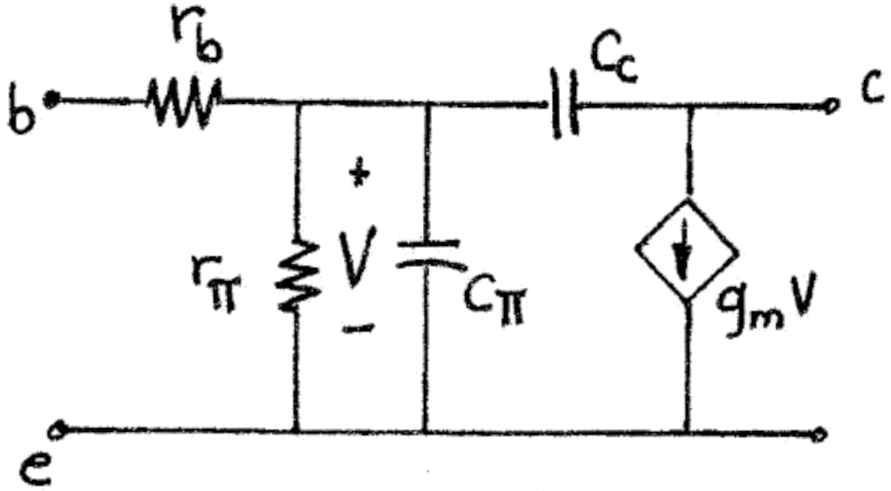
\includegraphics[width=0.5\linewidth]{_fig/respfreq_transistor-hibrido-simplificado.png}
	\caption{Modelo $\pi$ híbrido Simplificado}
	\label{fig:respfreq_transistor-hibrido-simplificado}
\end{figure}

Se ha relacionado los elementos del modelo $\pi$ híbrido a frecuencias bajas con los del modelo de los parámetros $h$; en caso que el fabricante de un transistor suministra valores de los parámetros $h$, de ellos se puede calcular los valores de los parámetros $g_m$, $r_{\pi}$ y $r_b$ del modelo simplificado.

\begin{figure}[h]
	\centering
	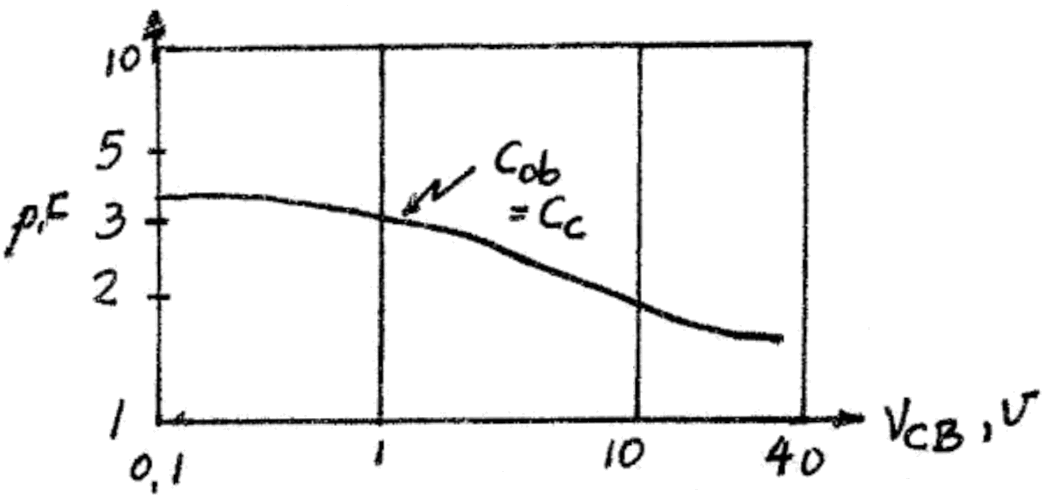
\includegraphics[width=0.5\linewidth]{_fig/respfreq_transistor-cap-junta-cb.png}
	\caption{Capacitancia de junta en función del voltaje $V_{CB}$}
	\label{fig:respfreq_transistor-cap-junta-cb}
\end{figure}

El valor de $C_c$ es inversamente proporcional al voltaje colector base. El fabricante generalmente especifica esta relación por medio de una gráfica entre las hojas de datos del transistor. Por ejemplo para el 2N3904 de Motorola aparece la gráfica de la Figura \ref{fig:respfreq_transistor-cap-junta-cb} para $C_{ob} = C_c$. Una ecuación que describe adecuadamente esta gráfica es:

\begin{equation}
	C_c \approx \frac{C_o}{(1 + V_{CB}/V_j)^{1/2}}
\end{equation}

donde $C_o$ es el valor de $C_c$ para $V_{CB} = 0$.

El valor de $c_\pi$ es función de $f_T$, donde $f_T$ es el producto ganancia ancho de banda de corriente para un transistor y su valor viene dado por el fabricante. $\omega_p$ se define como la frecuencia a la cual la ganancia de corriente baja a $1/\sqrt{2}$ de su valor máximo, con la salida en corto circuito; como se ve en la Figura \ref{fig:respfreq_transistor-salida-cortocircuito}. Se obtiene la corriente de salida, $I_o = -g_m v$. La transconductancia, $g_m$, no es función de la frecuencia; en cambio $v$ sí lo es.

\begin{figure}[h]
	\centering
	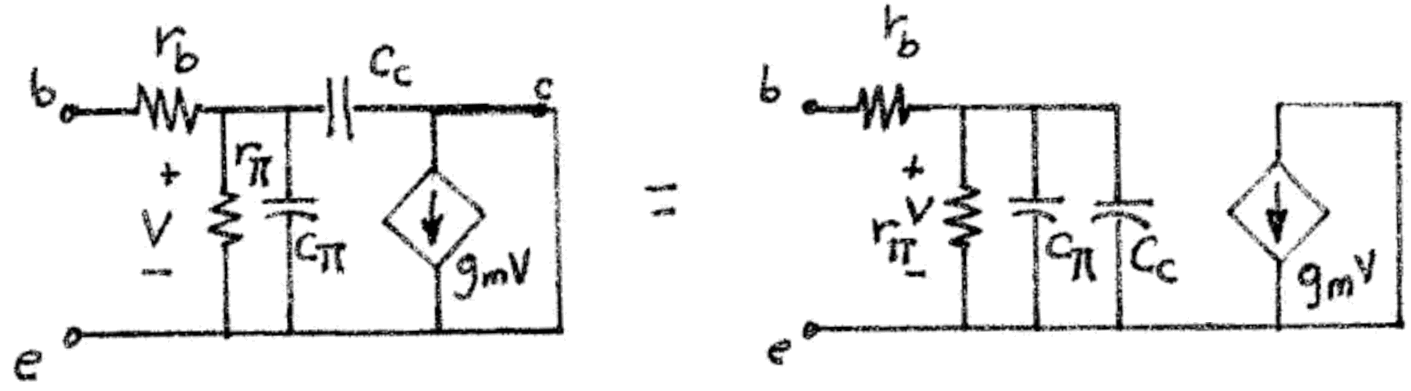
\includegraphics[width=0.8\linewidth]{_fig/respfreq_transistor-salida-cortocircuito.png}
	\caption{Modelo del Transistor con la Salida en Cortocircuito}
	\label{fig:respfreq_transistor-salida-cortocircuito}
\end{figure}

Se tiene que:

\[
I_i = v(g_{\pi} + s(C_{\pi} + C_c))
\]

\begin{equation}
	\frac{V}{I_i} = \frac{1}{(g_{\pi} + s(C_{\pi} + C_c))}
\end{equation}

e

\begin{equation}
	\frac{I_o}{I_i}(s) = \frac{-g_m V}{I_i} = \frac{-g_m}{g_{\pi} + s(C_{\pi} + C_c)}
\end{equation}

Esta función se grafica en la Figura \ref{fig:respfreq_transistor-corriente-funcion-omega}. La frecuencia de corte es:

\begin{equation} \label{respfreq_transistor_freq-corte}
	\omega_B = \frac{g_{\pi}}{C_{\pi} + C_c}
\end{equation}

\begin{figure}[h]
	\centering
	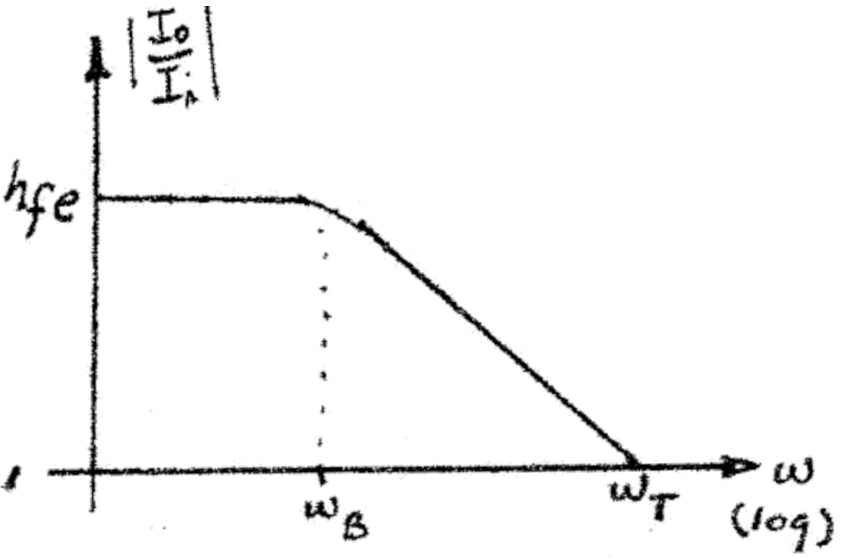
\includegraphics[width=0.8\linewidth]{_fig/respfreq_transistor-corriente-funcion-omega.png}
	\caption{Ganancia de Corriente en función de $\omega$}
	\label{fig:respfreq_transistor-corriente-funcion-omega}
\end{figure}

y entonces:

\[
\frac{I_o}{I_i}(s) = \frac{-g_m r_{\pi}}{1 + { S r_{\pi}  (C_{\pi} + C_C)} } = \frac{-\beta}{1 + s/\omega_B}
\]

A la frecuencia $\omega_T$ la ganancia baja por definición al valor de uno. A continuación se demuestra que esto ocurre para

\begin{equation} \label{respfreq_transistor_omega-t}
	\omega_T = \beta \omega_B \quad (1.61)
\end{equation}

pues entonces:

\[
\left| \frac{I_o}{I_i}(\omega_T) \right| = \frac{|-\beta|}{|1 + j \beta \omega_B / \omega_T|} \approx 1
\]

de la ecuación \ref{respfreq_transistor_omega-t} se entiende por que se conoce como el producto ganancia ancho de banda. De las ecuaciones \ref{respfreq_transistor_freq-corte} y \ref{respfreq_transistor_omega-t}, se tiene:

\begin{equation} \label{respfreq_transistor-pi-hibrido}
	\omega_T = \frac{\beta}{(C_{\pi} + C_c) r_{\pi}} = \frac{g_m}{C_{\pi} + C_c}
\end{equation}

de donde:

\begin{equation}
	C_{\pi} = \frac{g_m}{\omega_T} - C_c
\end{equation}

Se hace notar que en vista de que $g_m$ es función de $I_c$, el valor de $C_{\pi}$ es también función de $I_c$; aumenta con $I_c$.

En la Tabla \ref{tab:respfreq_modelo-hibrido} se resumen las ecuaciones utilizadas en la obtención de los valores de los elementos del modelo híbrido. La ecuación para $r_b$ carece de precisión al representar la pequeña diferencia entre dos valores grandes, y se establecen los siguientes límites.

\begin{equation}
	50 < r_b < 250
\end{equation}

de acuerdo a la gráfica que relaciona $r_b$ con $I_c$, la Figura \ref{fig:respfreq_transistor_rb-vs-ic}.

\begin{table}[h]
	\centering
	\begin{tabular}{|c|c|}
		\hline
		PARAMETRO & RELACION \\ \hline
		$g_m$ & $I_c q / V_T$ \\ \hline
		$r_{\pi}$ & $h_{fe} / g_m$ \\ \hline
		$r_b$ & $h_{ie} - r_{\pi}$ \\ \hline
		$C_c (V_{CB})$ & $C_o / (1+V_{CB}/V_j)^{1/2}$ \\ \hline
		$C_{\pi}$ & $g_m / \omega_T - C_c$ \\ \hline
	\end{tabular}
	\caption{Parámetros Modelo híbrido}
	\label{tab:respfreq_modelo-hibrido}
\end{table}

\begin{figure}[h]
	\centering
	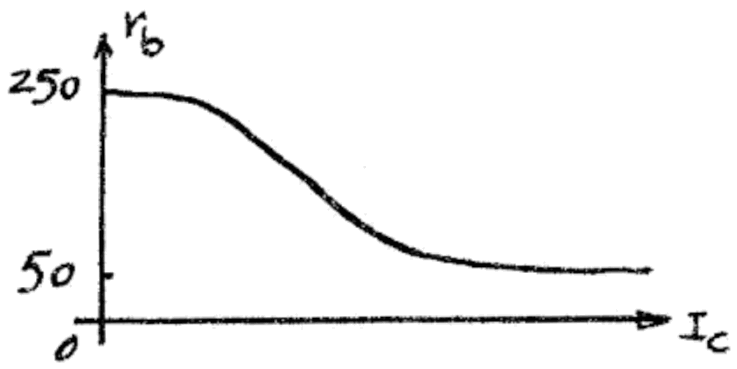
\includegraphics[width=0.8\linewidth]{_fig/respfreq_transistor_rb-vs-ic.png}
	\caption{$r_b$ vs $I_c$}
	\label{fig:respfreq_transistor_rb-vs-ic}
\end{figure}

\subsubsection{Ejemplo 5} \label{respfreq_ejm5}

Hallar los valores de los elementos del modelo híbrido para el circuito de la Figura \ref{fig:respfreq_ejemplo_t-ec_autopolarizado}; utilice $h_{fe} = 180$.

\begin{figure}[h]
	\centering
	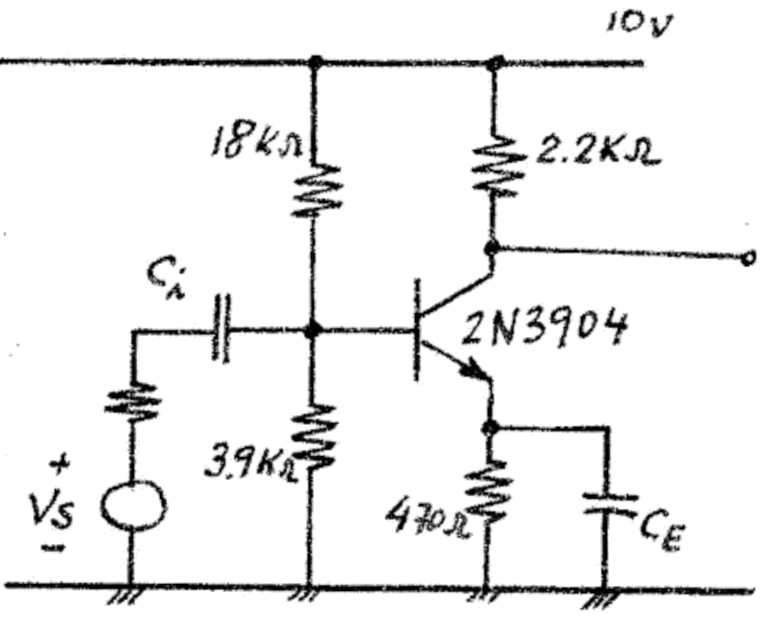
\includegraphics[width=0.8\linewidth]{_fig/respfreq_ejemplo_t-ec_autopolarizado.png}
	\caption{Amplificador EC autopolarizado}
	\label{fig:respfreq_ejemplo_t-ec_autopolarizado}
\end{figure}

\textbf{Solución:}

\textbf{a)} Hallar $V_{CE}$ e $I_C$

Sacando el equivalente de Thevenin en continua en la base nos da:

\[
1.78V = I_B \times 32K + 0.6V + (181) I_B \times 470
\]

ó $I_B = 23.3 \mu A$ e $I_C = 2.33 mA$

Con las hojas de datos del 2N3904 y el valor $I_C = 2.3 mA$, encontramos los valores de $h_{fe} = 150$ y $h_{ie} = 1800$.

Entonces:

\[
g_m = \frac{I_C}{V_T} = \frac{2.33 mA}{26 mV} = 0.0896 mho
\]

\[
r_{\pi} = \frac{\beta}{g_m} = \frac{150}{0.0896} = 1670 \Omega
\]

\[
r_b = h_{ie} - r_{\pi} = 130 \quad \text{(está dentro de los límites)}
\]

Después para $C_c$ hallamos primero $V_{CB} = V_{CE} - V_{BE}$

donde \( V_{CE} = V_{CC} - I_C R_L - I_E R_E \)

\[ V_{CE} = 10 - 2.33 (2.2 + 0.47) = 3.78 V \]

es decir \( V_{CB} = 3.18 V \) y \( C_C (3.18 V) \approx 2 pF \)

Luego:

\( C_{\pi} = \frac{g_m}{\omega_T} - C_c \), \(\omega_T = 2 \pi f_T\) y \(f_T = 300 MHz\) para el 2N3904; por lo tanto \( C_{\pi} = \frac{0.896}{2 \pi 3 \times 10^8} - 2 \times 10^{-12} = 45.5 pF \)

El circuito de la Figura \ref{fig:respfreq_ejemplo_t-ec_autopolarizado} queda con el modelo de la Figura \ref{fig:respfreq_ejemplo_t-ec_ac} para corriente alterna.

\begin{figure}[h]
	\centering
	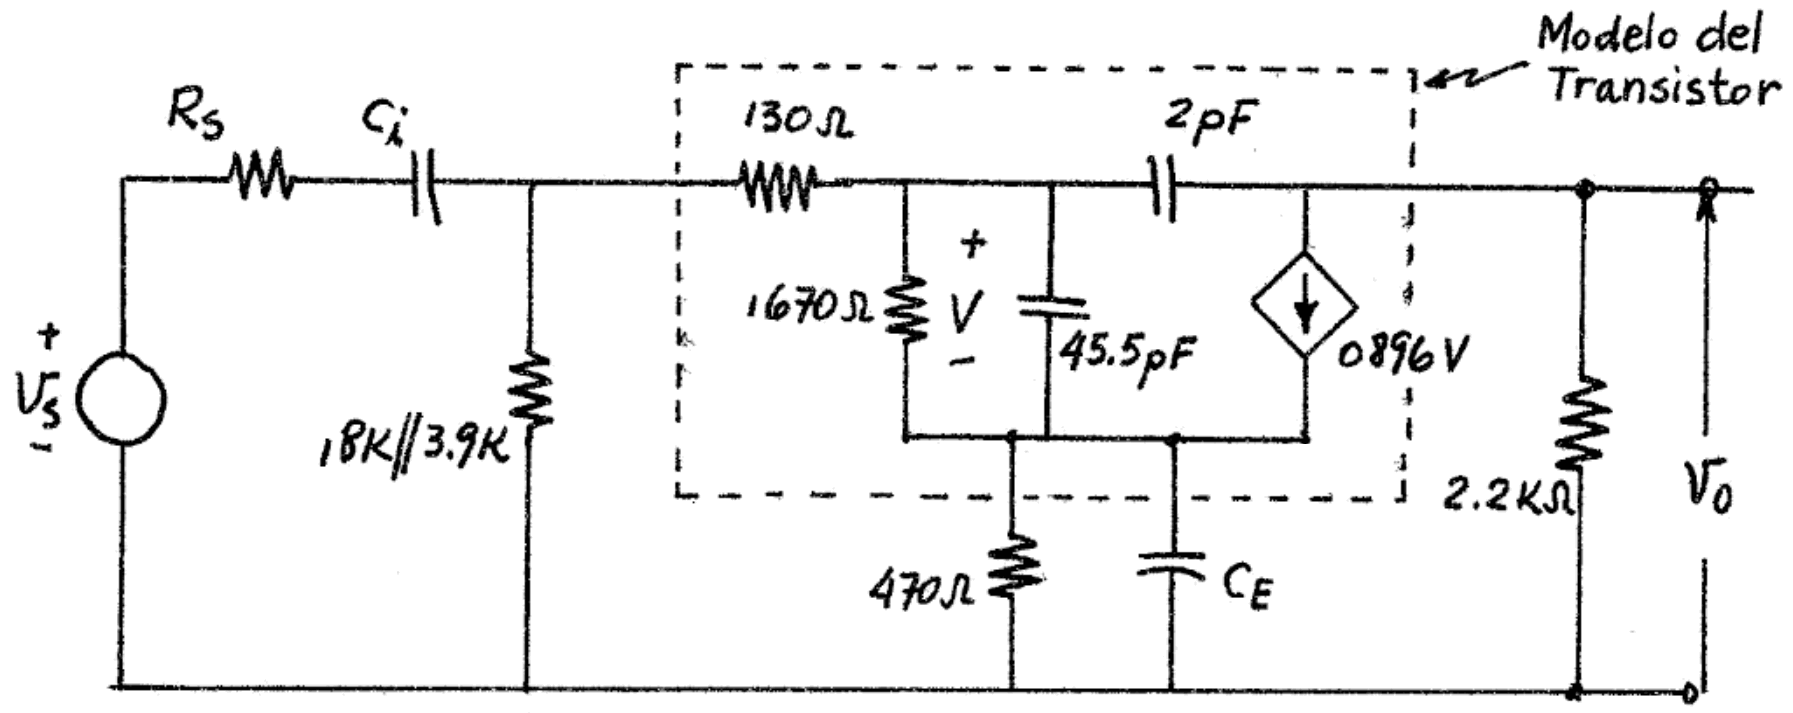
\includegraphics[width=0.8\linewidth]{_fig/respfreq_ejemplo_t-ec_ac.png}
	\caption{El circuito de la Figura \ref{fig:respfreq_ejemplo_t-ec_autopolarizado} para C.A.}
	\label{fig:respfreq_ejemplo_t-ec_ac}
\end{figure}

Se tiene un modelo de alta frecuencia, y se aplica una configuración emisor común para determinar la respuesta de frecuencia para altas frecuencias, como se indica en la Figura \ref{fig:respfreq_emisor-comun-autolarizado_c-short}.

Se quiere la función de transferencia \( V_O / V_S (s) \). Se hace la observación que en el circuito \( (c) \) a analizar, hay menos nodos que mallas, y por lo tanto es más rápido el análisis por ecuaciones de nodo que por ecuaciones de malla. Se tiene 3 nodos: \( b' \), \( c \), y tierra, por lo que se tiene que plantear dos ecuaciones de nodo:

en \( b' \):

\[ V (g_{\pi} + S C_{\pi}) + (V - V_S) g_b' + (V - V_o) S C = 0 \]

en c:

\begin{equation}			
	(V_o - V) s C_c + g_m V + V_o G_L = 0
\end{equation}

Separando los coeficientes de las incógnitas:

\begin{equation}			
	V (g_{\pi} + s C_{\pi} + g_b') + (-s C_c) + V_o (-s C_c) = g_b' V_S'
\end{equation}
\begin{equation}			
	V (g_m - s C_c) + V_o (s C_c + G_L) = 0
\end{equation}

Se puede utilizar la regla de Cramer para despejar \( V_o \):

\begin{equation}
	V_o = \frac{
		\begin{vmatrix}
			g_{\pi} + s C_{\pi} + g_b' + s C_c & g_b' V_S' \\
			g_m - s C_c & 0
		\end{vmatrix}
	}{
		\begin{vmatrix}
			g_{\pi} + s C_{\pi} + g_b' + s C_c & -s C_c \\
			g_m - s C_c & s C_c + G_L
		\end{vmatrix}
	}
\end{equation}

\begin{figure}[h]
	\centering
	\subfloat[Configuración E.C.]
	{
		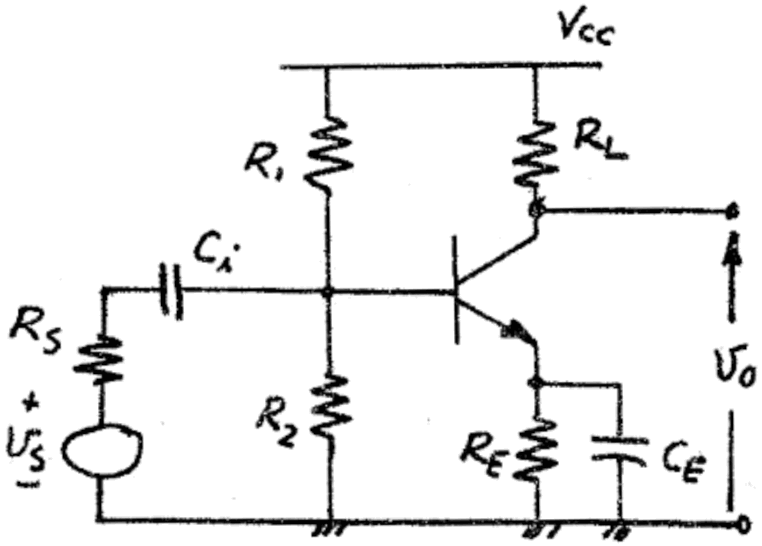
\includegraphics[width=0.26\linewidth]{_fig/respfreq_ejemplo_t-hf-ec_conf.png}
		\label{fig:respfreq_ejemplo_t-hf-ec_conf}
	}
	\subfloat[Circuito para frecuencias medias y altas]
	{
		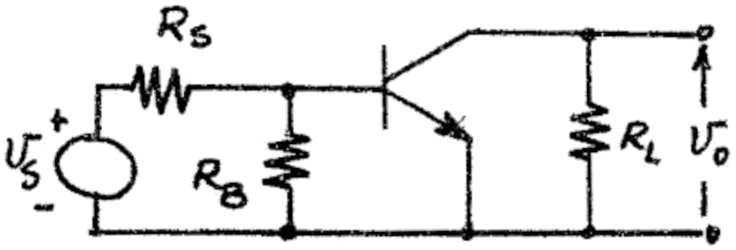
\includegraphics[width=0.33\linewidth]{_fig/respfreq_ejemplo_t-hf-ec_mf-hf.png}
		\label{fig:respfreq_ejemplo_t-hf-ec_mf-hf}
	}
	\subfloat[Circuito con Modelo]
	{
		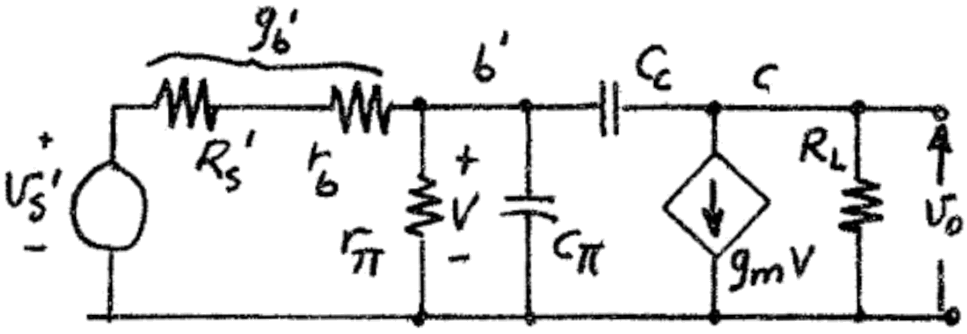
\includegraphics[width=0.37\linewidth]{_fig/respfreq_ejemplo_t-hf-ec_con-modelo.png}
		\label{fig:respfreq_ejemplo_t-hf-ec_con-modelo}
	}
	\caption{Análisis de Alta Frecuencia para E.C.}
	\label{fig:respfreq_ejemplo_t-hf-ec}
\end{figure}

de donde:

\[ V_o = \frac{-g_b' V_S' (g_m - s C_c)}{(g_\pi + s C_\pi + g_b' + {s C_c}) (s C_c + G_L) - (-s C_c) (g_m - s C_c)} \]

ó,

\begin{equation} \label{respfreq_transistor_funcion-transferencia}
	\frac{V_o}{V_S'} (s) = \frac{-g_b' (g_m - s C_c)}{s^2 C_\pi C_c + s (C_\pi G_L + C_c (g_m + G_L g_\pi + G_L g_b)) + (g_\pi + g_b') G_L}
\end{equation}

Esta es la función de transferencia completa para medias y altas frecuencias de donde se puede hallar los polos y los ceros de \( V_o / V_S' (s) \).

Se ha demostrado que el modelo híbrido es solo válido para

\begin{equation} \label{respfreq_transistor-pi-hibrido_valido}
	\omega < \omega_T / 3
\end{equation}

Mas alla de esta frecuencia, se requiere de modelos mas sofisticados del transistor. Dado la ecuación \ref{respfreq_transistor-pi-hibrido}, la ecuación \ref{respfreq_transistor-pi-hibrido_valido} es equivalente a:

\begin{equation}
	\omega < \frac{g_m}{(C_\pi + C_c) 3}
\end{equation}

Expresado de otra forma, el modelo híbrido es válido solo para:

\begin{equation}
	\omega C_c + \omega C_\pi << g_m
\end{equation}

que a su vez implica:

\begin{equation}
	\omega C_\pi << g_m
\end{equation}

\begin{equation}
	\omega C_c << g_m
\end{equation}

De la ecuación \ref{respfreq_transistor_funcion-transferencia} se puede despreciar el termino \( s^2 C_\pi C_c \) ya que \( s^2 C_\pi C_c << g_m s C_c \) y se desprecia en el numerador \( s C_c \). Entonces queda:

\begin{equation}
	\frac{V_o (s)}{V_S} \approx \frac{-g_m g_m}{s [C_\pi G_L + C_c (g_m + G_L + g_b')] + (g_\pi + g_b') G_L}
\end{equation}

Para expresarlo de la forma deseada, \( V_o (s) = K \frac{1}{1 + s \tau} \), sacamos el factor \( G_L (g_\pi + g_b') \) y queda:

\begin{equation} \label{respfreq_transistor_funcion-transferencia_vo-ss}
	\frac{V_o (s)}{V_S} = \frac{-g_m g_m R_L}{g_\pi + g_b'} \frac{1}{1 + s \frac{C_\pi + C_c (1 + R_L (g_m + g_b'))}{g_\pi + g_b'}}
\end{equation}

Por lo tanto, el polo de alta frecuencia viene dado por:

\begin{equation} \label{respfreq_transistor_gain-hf}
	\omega_A = \frac{1}{R_T C_A} = \frac{g_\pi + g_b'}{C_\pi + C_c (1 + R_L (g_m + g_\pi + g_b'))}
\end{equation}

La ganancia a frecuencias medias viene dada por:

\begin{equation} \label{respfreq_transistor_gain-mf}
	A = \frac{-g_m R_L}{g_\pi + g_b'} = -\frac{g_m R_L}{1/r_\pi + 1/R_S'} = \frac{-\beta R_L}{r_\pi + R_S'}
\end{equation}

Esta expresión es la misma que se consigue para la ganancia de la configuración E.C. utilizando el modelo simplificado.

\begin{figure}[h]
	\centering
	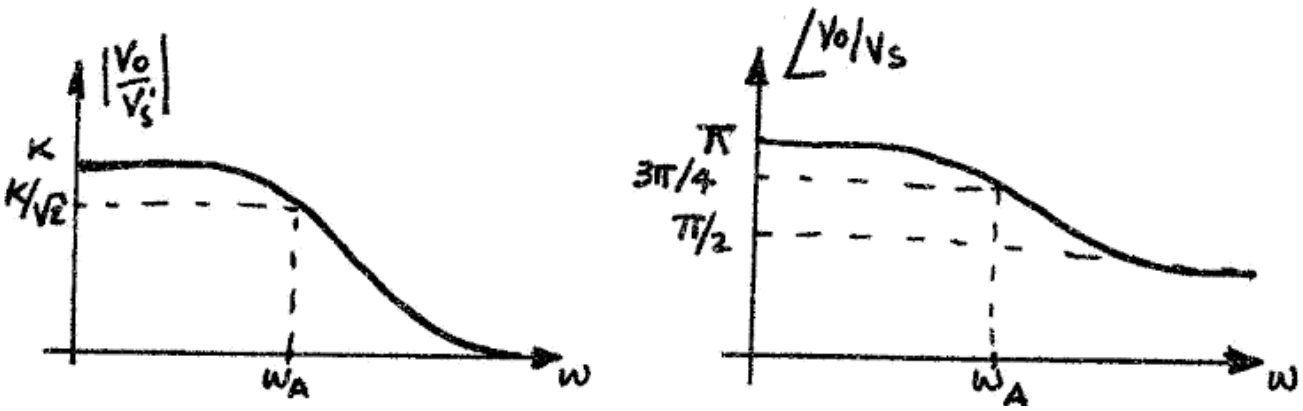
\includegraphics[width=0.8\linewidth]{_fig/respfreq_ejemplo_resp_funcion-transferencia.png}
	\caption{Respuesta de la Funcion de la Ecuación \ref{respfreq_transistor_gain-mf}}
	\label{fig:respfreq_ejemplo_resp_funcion-transferencia}
\end{figure}

En la Figura \ref{fig:respfreq_ejemplo_resp_funcion-transferencia} se muestra la respuesta de la Ecuación \ref{respfreq_transistor_funcion-transferencia_vo-ss}. Si ahora se toma en cuenta la contribución a la función de transferencia debido a \( C_i \) y \( C_E \) se consigue:

\begin{equation} \label{respfreq_transistor_resp-equ}
	\frac{V_o}{V_S} (s) = K \frac{s}{s + \omega_1} \frac{s \omega_2}{s + \omega_3} \frac{1}{1 + s \tau_A}
\end{equation}

\begin{figure}[h]
	\centering
	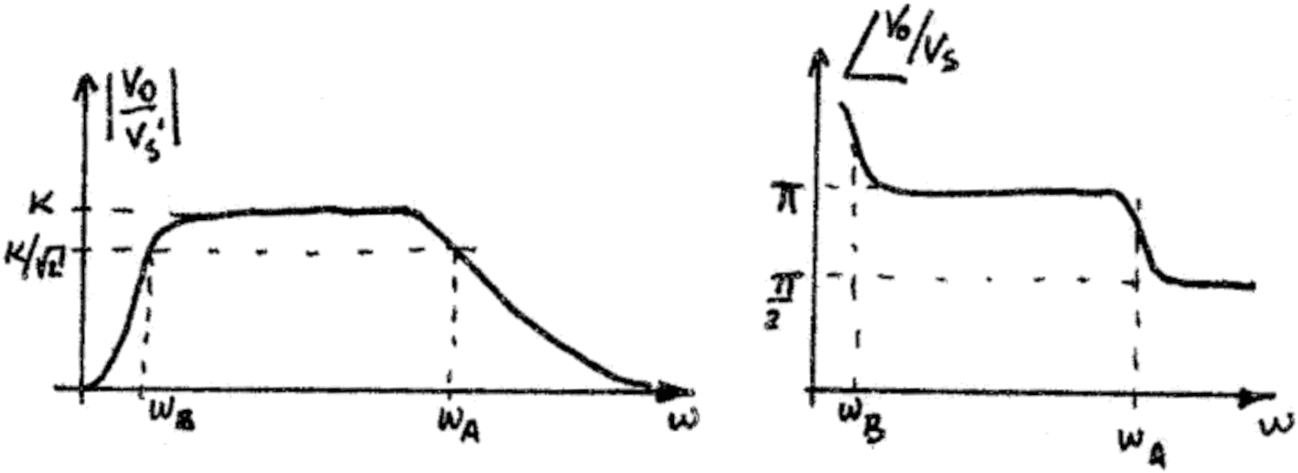
\includegraphics[width=0.8\linewidth]{_fig/respfreq_ejemplo_resp_funcion-transferencia-eq.png}
	\caption{Respuesta de la Función de la Ecuación \ref{respfreq_transistor_resp-equ}}
	\label{fig:respfreq_ejemplo_resp_funcion-transferencia-eq}
\end{figure}

que se grafica en la Figura \ref{fig:respfreq_ejemplo_resp_funcion-transferencia-eq}.

Además la expresión para la frecuencia de corte alta, la Ecuación \ref{respfreq_transistor_gain-hf}, tiene una interpretación circuital muy interesante.

donde \( g_\pi + g_b' = \frac{1}{r_\pi \parallel R_S'} \). Y se desprecia \( g_\pi + g_b' \) que generalmente cumplen la condición \( g_\pi + g_b' << g_m \). El circuito que tiene este polo, y la ganancia dada en la Ecuación \ref{respfreq_transistor_gain-mf} se muestra en la Figura \ref{fig:respfreq_resp-simple-conf-ec}. El polo viene dado por \(-1 / R_T C_T\) donde \( R_T \) es la resistencia de Thevenin vista desde los extremos de la capacitancia total:

\[ C_\pi + C_c (1 + g_m R_L) \]

\begin{figure}[h]
	\centering
	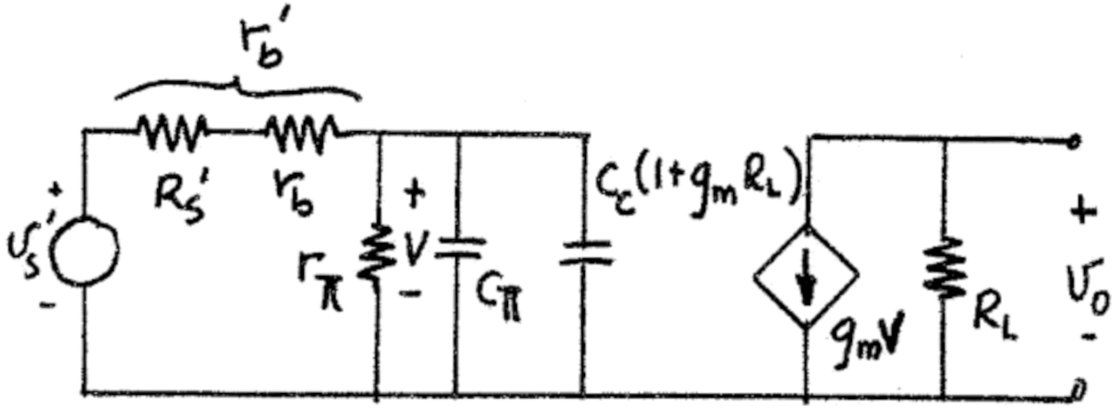
\includegraphics[width=0.8\linewidth]{_fig/respfreq_resp-simple-conf-ec.png}
	\caption{Interpretación circuital sencilla para configuración E.C.}
	\label{fig:respfreq_resp-simple-conf-ec}
\end{figure}

La capacitancia \( C_c (1 + g_m R_L) \) forma parte de la capacitancia de entrada y domina la capacitancia de Miller ya que corresponde a la calculada partiendo del Teorema de Miller, planteado en la Figura \ref{fig:respfreq_teorema-miller}. El teorema establece que las tensiones y corrientes en una red permanecen iguales si cualquier impedancia Z entre dos nodos con voltajes \( V_1 \) y \( V_2 \), se transforma en dos impedancias a tierra de valores \( Z' = Z / (1 - V_2 / V_1) \) del nodo \( V_1 \), y \( Z'' = Z / (1 - V_1 / V_2) \) del nodo \( V_2 \).

\begin{figure}[h]
	\centering
	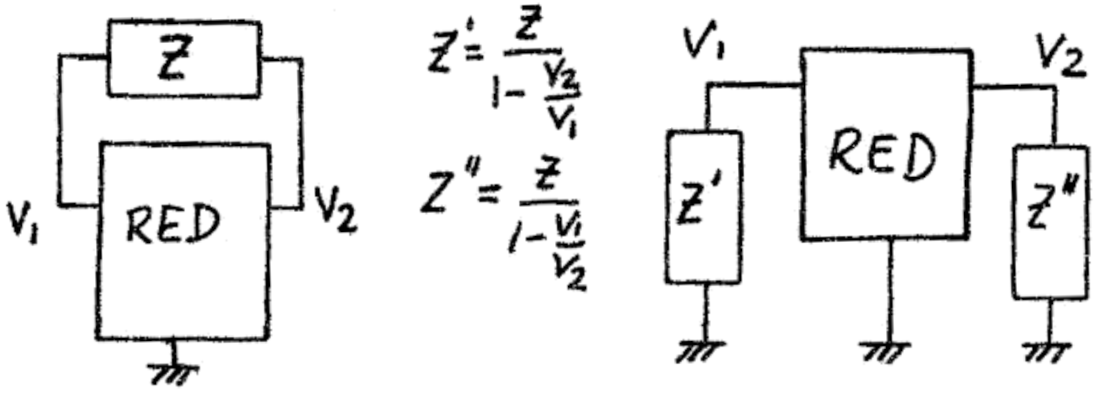
\includegraphics[width=0.8\linewidth]{_fig/respfreq_teorema-miller.png}
	\caption{Teorema de Miller}
	\label{fig:respfreq_teorema-miller}
\end{figure}

Del circuito de la Figura \ref{fig:respfreq_ejemplo_t-hf-ec_con-modelo}, se determina que la ganancia \( V_o / V = -g_m R_L \). Entonces se puede llevar \( C_c \) a su equivalente en paralelo con \( C_\pi \) con valor \( C_c (1 + g_m R_L) \) ya que:

\[ Z' = \frac{Z}{1 - \frac{V_o}{V}} = \frac{1}{s C_c (1 - (-g_m R_L))} = \frac{1}{s C (1 + g_m R_L)} \]

A pesar de que \( C_c \) es una capacitancia pequeña su efecto sobre el polo de alta frecuencia es tan apreciable como \( C_\pi \) debido al factor multiplicador \( (1 + g_m R_L) \).

Se hace notar que aplicando el Teorema de Miller se crea otra capacitancia en paralelo con \( R_L \), pero su efecto es despreciable como veremos en el próximo ejemplo.

\subsubsection{Ejemplo 6} \label{respfreq_ejm6}
Hallar la ganancia y la frecuencia de corte alta para el circuito de la Figura \ref{fig:respfreq_ejemplo_t-ec_autopolarizado}.

\textbf{Solución.} En la figura 1.61 se plantea el circuito apto para este análisis, en donde se parte del circuito de la figura 1.55 con los condensadores \( C_i \) y \( C_E \) cortocircuitados, y con \( R_S = 50 \).

\begin{figure}[h]
	\centering
	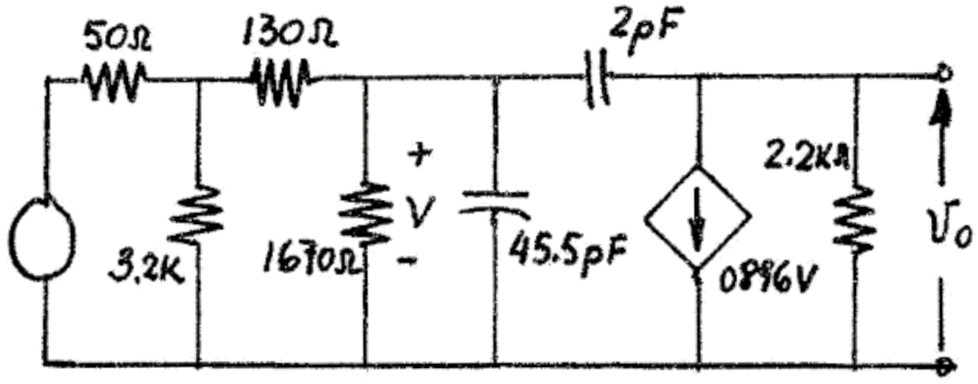
\includegraphics[width=0.8\linewidth]{_fig/respfreq_ejemplo_t-ec_autopolarizado_mf-hf.png}
	\caption{Circuito de la Figura \ref{fig:respfreq_ejemplo_t-ec_autopolarizado} para medias y altas frecuencias}
	\label{fig:respfreq_ejemplo_t-ec_autopolarizado_mf-hf}
\end{figure}

Entonces:

\[ A_M = \frac{-\beta R_L}{r_\pi + R_S} = \frac{-150 \times 2.2 \text{ k}}{1800 + 99.2} = -178 \]

el polo dominante:

\[ \omega_A = \frac{g_\pi + g_b'}{C_\pi + C_c (1 + g_m + g_\pi + g_b') R_L} \]

\[ \omega_A = \frac{0.00618}{45.1 \times 10^{-12} + 2.2 \times 10^{-12} (1 + (0.00618 + 0.0896) 2.2 \times 10^3)} = 13.2 \text{ MR/s } (f_A = 2.1 \text{ MHz}) \]

y el segundo polo:

\[ \omega_{A2} = \frac{1}{R_L C_c} = \frac{1}{2.2 \times 10^3 \times 2 \times 10^{-12}} = 227 \text{ MR/s } (\text{casi } 20 \omega_A) \]

\subsubsection{Ejemplo 7} \label{respfreq_ejm7}
Si \( R_L \) cambia a \( 1.1K \), con \( I_C \) igual y \( V_{CE} = 5.6 \) se tiene \( C_c = 1.9 pF \). Entonces, \( A_M = -89 \) y \( \omega_A = 25 MR/s \).

Una comparación de las ganancias y frecuencias de corte alta obtenidas en los Ejemplos \ref{respfreq_ejm6} y \ref{respfreq_ejm7} demuestra la relación inversa entre ganancia y ancho de banda que siempre se presenta en los amplificadores electrónicos: si uno aumenta, la otra disminuye.

\subsubsection{Ejemplo 8} \label{respfreq_ejm8}
Hallar la función de transferencia general y los valores específicos de la ganancia y la frecuencia de corte alta de la configuración colector común de la Figura \ref{fig:respfreq_conf-colector-comun}.

\begin{figure}[h]
	\centering
	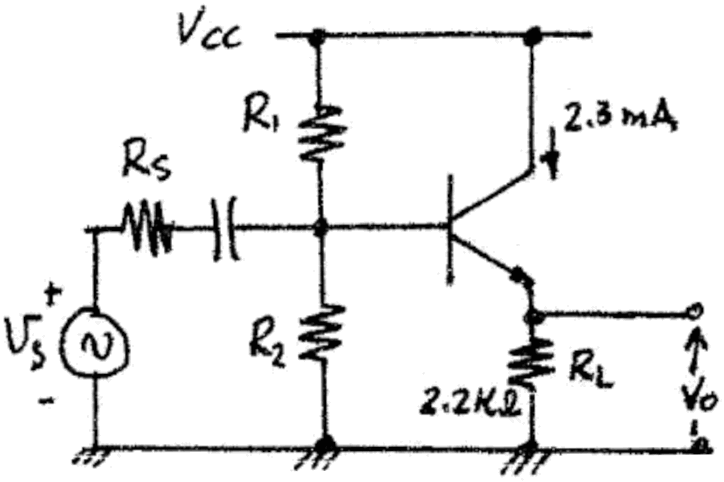
\includegraphics[width=0.5\linewidth]{_fig/respfreq_conf-colector-comun.png}
	\caption{Configuración Colector Común}
	\label{fig:respfreq_conf-colector-comun}
\end{figure}

El mismo procedimiento que se aplicó a la configuración E.C. se podría aplicar ahora a las demás configuraciones.

Para altas, el circuito de la Figura \ref{fig:respfreq_conf-colector-comun} queda como en la Figura \ref{fig:respfreq_conf-colector-comun_hf}.

\begin{figure}[h]
	\centering
	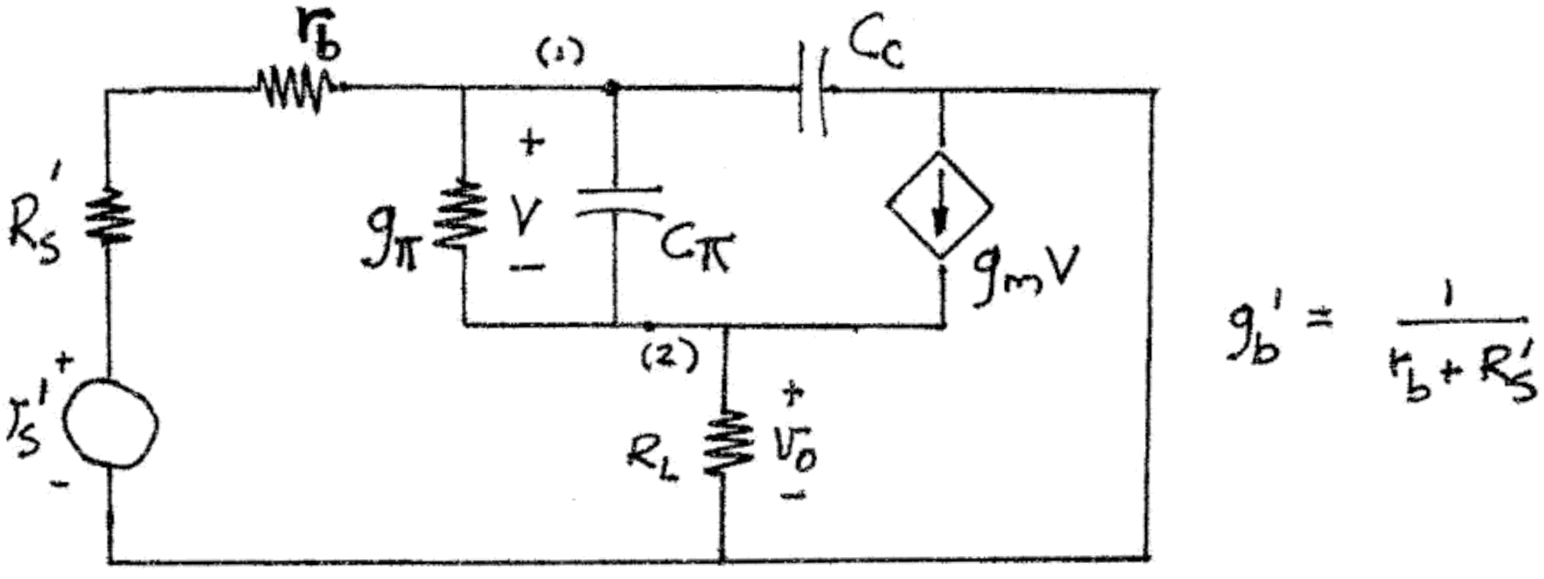
\includegraphics[width=0.8\linewidth]{_fig/respfreq_conf-colector-comun_hf.png}
	\caption{Amplificador Configuración Colector Común para Altas Frecuencias}
	\label{fig:respfreq_conf-colector-comun_hf}
\end{figure}

Entonces:

1) \( (V + V_o - V_S) g_b' + V (g_\pi + s C_\pi) + (V + V_o) s C_c = 0 \)

2) \( -V(g_\pi + s C_\pi + g_m) + V_o g_L = 0 \)

Luego:

1) \( V(g_b' + g_\pi + sC_c) + V_o(g_b' + sC_c) = V_s' g_b' \)

2) \( V = \frac{V_o g_L}{g_\pi + sC_\pi + g_m}  \approx \frac{V_o g_L}{g_m} \)

Finalmente:

\[ V_o \left[ \frac{g_L (g_b' + g_\pi + sC_c + sC_\pi)}{g_m} + g_b' + s C_c \right] = V_s' g_b' \]

ó

\[ \frac{V_o}{V_s'} = \frac{g_m g_b'}{g_L (g_b' + g_\pi) + g_m g_b' + g_L (s C_c + s C_\pi) + g_m s C_c} \]

de donde

\[ \frac{V_o}{V_s'} = \frac{g_m g_b'}{g_L (g_b' + g_\pi) + g_m g_b'} \frac{1}{1 + s \left[ \frac{g_L (C_c + C_\pi) + g_m C_c}{g_L (g_b' + g_\pi) + g_m g_b'} \right]} \]

\[ \frac{V_o}{V_s'} = A_M \frac{1}{1 + s \tau_A} \]

Dado valores del Ejemplo \ref{respfreq_ejm2} (caso E.C.) y \( R_L = 2.2K \), se obtiene \( g_L = 0.000455 \), \( g_m = 0.0896 \), \( g_b' = 0.00558 \), \( g_\pi = 0.0006 \), \( C_c = 2.4 pF \), \( C_\pi = 45.1 pF \). Entonces:

\[ A_M = \frac{0.0896 + 0.00558}{0.000455 (0.00558 + 0.0006) + (0.0896) (0.00558)} = 0.999 \]

\[ \omega_A = \frac{0.000455 (0.00558 + 0.0006) + (0.0896) (0.00558)}{(0.000455) (47.5 \times 10^{-12}) + (0.0896) (2.4 \times 10^{-12})} = 2.1 \times 10^9 \]

\section{Problemario} %p59
- pendiente en apuntes -	% Respuesta de frecuencia de circuitos electrónicos
	% Licencia y derechos: consulte ../../LICENSE-CC-BY-4.0.
% Las figuras y demás materiales de terceros pueden tener derechos separados y deben identificarse.

\chapter{Amplificadores de varias etapas} %p70

En el capítulo anterior, se demostró una relación inversa entre ganancia y ancho de banda cuando se analizó el amplificador emisor común para altas frecuencias. Esto es indicativo de los límites en los posibles alcances con una sola etapa. En el presente capítulo se estudiará configuraciones de varias etapas que permitirán mejorar las características del conjunto, como por ejemplo, aumentar la impedancia de entrada de un amplificador u obtener una mayor frecuencia de corte alta para una ganancia dada. También se verá como puede acoplarse etapas directamente para así amplificar corriente continua. En este aspecto saldrá a relucir la configuración diferencial, la cual se analizará a fondo. Finalmente se presentarán amplificadores comerciales fabricados como circuitos integrados que también amplifican en corriente continua.

\section{Sistemas de varias etapas: Generalidades} %p70

En la Figura \ref{fig:multietapas_sistema-cascada} se plantea un sistema de varias etapas en cascada. Las características de mayor interés de un sistema son la ganancia de voltaje, \( A_V \), la ganancia de corriente, \( A_I \), la resistencia de entrada \( R_i \), la resistencia de salida \( R_o \) y el rango de frecuencias de operación del sistema.

\begin{figure}[h]
	\centering
	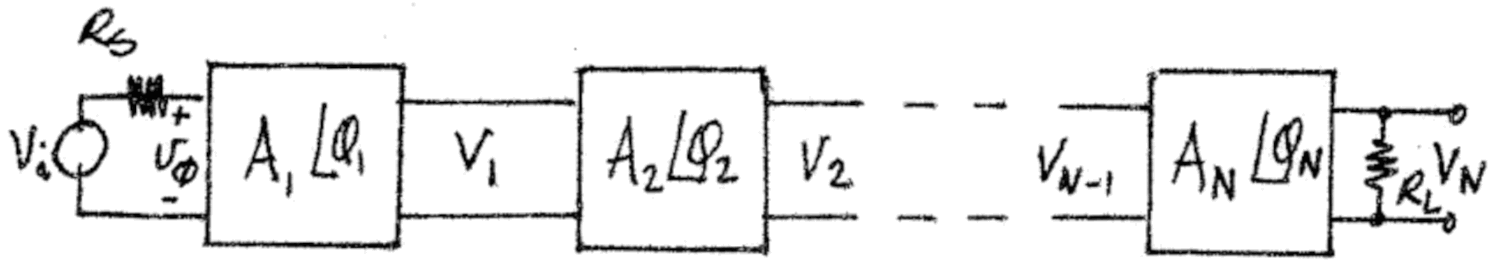
\includegraphics[width=0.8\linewidth]{_fig/multietapas_sistema-cascada.png}
	\caption{Sistema de varias Etapas en Cascada}
	\label{fig:multietapas_sistema-cascada}
\end{figure}

En el sistema:

\begin{equation}
	\frac{V_o}{V_s} (\omega) = \frac{R_i}{(R_{i1} + R_s)} = A_{\phi} (\omega) \angle \phi_{\phi} (\omega)
\end{equation}

\begin{equation}
	\frac{V_N}{V_{N-1}} (\omega) = A_N (\omega) \angle \phi_N (\omega)
\end{equation}

Después los totales vienen dados por:

\begin{equation}
	\left| \frac{V_N}{V_s} \right| = \left| \frac{V_N}{V_{N-1}} \right| \left| \frac{V_{N-1}}{V_{N-2}} \right| \cdots \left| \frac{V_i}{V_{\phi}} \right| \left| \frac{V_{\phi}}{V_s} \right| = A_N A_{N-1} \cdots A_1 A_{\phi}
\end{equation}

\begin{equation}
	\angle \frac{V_N}{V_s} = \phi_N + \phi_{N-1} + \cdots + \phi_1 + \phi_0
\end{equation}

La ganancia en forma logarítmica queda como una suma:

\begin{equation}
	\log \left| \frac{V_N}{V_s} \right| = \log A_N + \log A_{N-1} + \cdots + \log A_1 + \log A_{\phi}
\end{equation}

Para un amplificador con flujo de señal unilateral, se plantea un modelo general, como se muestra en la Figura \ref{fig:multietapas_rep-amp}.

\begin{figure}[h]
	\centering
	\subfloat[Modelo general]
	{
		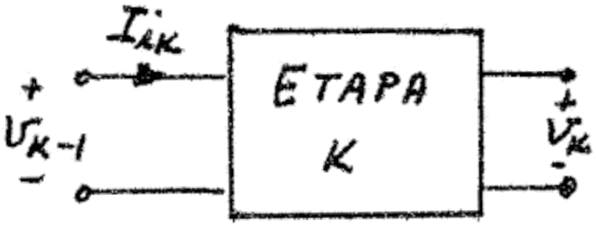
\includegraphics[width=0.32\linewidth]{_fig/multietapas_rep-amp_modelo-general.png}
		\label{fig:multietapas_rep-amp_modelo-general}
	}
	\subfloat[Basado en fuente de voltaje controlado]
	{
		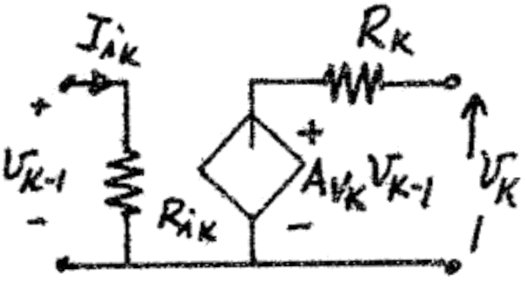
\includegraphics[width=0.32\linewidth]{_fig/multietapas_rep-amp_voltaje-controlado.png}
		\label{fig:multietapas_rep-amp_voltaje-controlado}
	}
	\subfloat[Basado en fuente de corriente controlado]
	{
		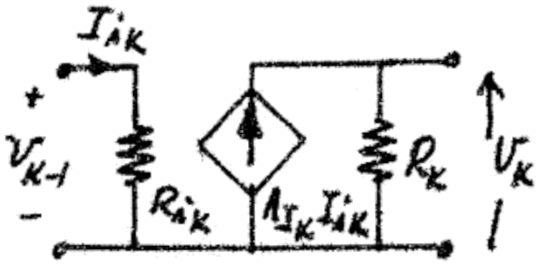
\includegraphics[width=0.32\linewidth]{_fig/multietapas_rep-amp_corriente-controlado.png}
		\label{fig:multietapas_rep-amp_corriente-controlado}
	}
	\caption{Representaciones de Amplificadores}
	\label{fig:multietapas_rep-amp}
\end{figure}

En la Figura \ref{fig:multietapas_rep-amp}, \( A_{Ik} \) es la ganancia de corriente de la etapa con la salida en corto circuito, y \( A_{Vk} \) es la ganancia de tensión de la etapa sin carga. Se consigue:

\begin{equation}
	V_k = A_{Ik} I_{ik} R_k
\end{equation}

también

\begin{equation}
	I_{ik} = V_{k-1} / R_{ik}
\end{equation}

y la relación entre ganancia de voltaje y corriente viene dada por:

\begin{equation}
	A_{Vk} = \frac{V_k}{V_{k-1}} = A_{Ik} \frac{R_k}{R_{ik}}
\end{equation}

Al anexar otra etapa, vea la Figura \ref{fig:multietapas_conexion-otra-etapa}, se cae la ganancia inter-etapas.

\begin{equation}
	A_K = \frac{V_K}{V_{K-1}} = \frac{R_{i(K+1)}}{R_{i(K+1)} + R_K} A_{VK}
\end{equation}

ademas

\begin{equation}
	A_K' = \frac{I_{i(K+1)}}{I_{ik}} = A_{IK} \frac{R_K}{R_K + R_{i(K+1)}}
\end{equation}

\begin{figure}[h]
	\centering
	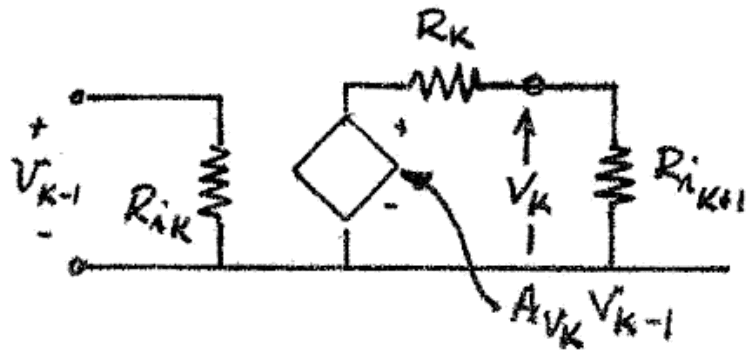
\includegraphics[width=0.8\linewidth]{_fig/multietapas_conexion-otra-etapa.png}
	\caption{Conexión de otra etapa}
	\label{fig:multietapas_conexion-otra-etapa}
\end{figure}

La ganancia de voltaje total, \( A_{VT} \), viene dada por

\begin{equation}
	A_{VT} = \frac{A_{IT} R_L}{R_S + R_{i1}}
\end{equation}

donde \( A_{IT} \) es la ganancia de corriente total y viene dada por

\begin{equation}
	A_{IT} = A_{I1} A_{I2} \cdots A_{IN}'
\end{equation}

En general la resistencia de salida del conjunto es la resistencia de salida de la última etapa, y la resistencia de entrada es la de la primera etapa.

\section{La configuración Darlington} %p72

La Configuración Darlington, que se muestra en la Figura \ref{fig:multietapas_conf-darlington}, está formado por dos transistores que conforman un super-transistor, es decir representan un dispositivo de tres contactos cuya ganancia de corriente es aproximadamente el cuadrado de la de un solo transistor.

\begin{figure}[h]
	\centering
	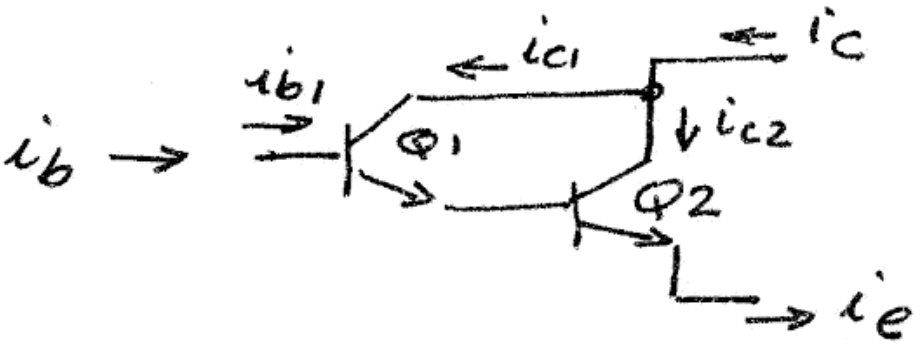
\includegraphics[width=0.8\linewidth]{_fig/multietapas_conf-darlington.png}
	\caption{Configuración Darlington}
	\label{fig:multietapas_conf-darlington}
\end{figure}

Partiendo de este diagrama se obtienen las siguientes ecuaciones:

\[ i_c = i_{c1} + i_{c2} \]
\[ i_{c1} = \beta_1 i_{b1} \]
\[ i_{b2} = (\beta_1 + 1) i_{b1} \]
\[ i_c = \beta_1 i_{b1} + \beta_2 i_{b2} = \beta_1 i_{b1} + \beta_2 (\beta_1 + 1) i_{b1} \]

para eventualmente llegar a:

\begin{equation}
	i_c = [\beta_1 + \beta_1 \beta_2 + \beta_2] i_{b1} = (\beta+2)\beta i_b
\end{equation}

De aquí se desprende que la relación entre la corriente de "colector" y la corriente de base es \( \beta + 2 \) veces mayor que esta relación para una sola etapa. Si para una etapa la \( \beta \) es 100, con la configuración Darlington, la "\( \beta \)" es mas de 10.000.

\subsection{Ejemplo 1} \label{multietapas_ejm1}
Para el circuito de la Figura \ref{fig:multietapas_conf-darlington_colector-comun}, determine a) la corriente de base de entrada en continua, y b) la resistencia de entrada. Utilice \( \beta = 100 \) para los transistores.

\begin{figure}[h]
	\centering
	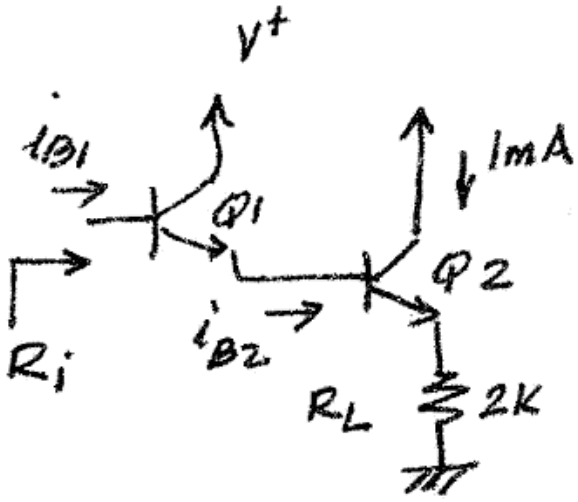
\includegraphics[width=0.5\linewidth]{_fig/multietapas_conf-darlington_colector-comun.png}
	\caption{Configuración Darlington como Colector Común}
	\label{fig:multietapas_conf-darlington_colector-comun}
\end{figure}

\textbf{Solución.}

Dado que la corriente por \( R_L = 1 mA\) , entonces la corriente de base de Q2 \( I_{BQ2} = 10 \mu A\) , y la corriente de base de Q1 \( I_{BQ1} \approx 0.1 \mu A\) . Por lo tanto,

\[ r_{\pi 1} = \frac{\beta}{g_{m1}} = \frac{100 \times 25 mV}{100 \mu A} = 250 k\Omega \]

\[ r_{\pi 2} = 2.5 k\Omega \]

y

\[ R_L = r_{\Pi 1} + (\beta_1 +1) \left[ (r_{\Pi 2} + (\beta_1 +1) R_L \right] = 20.9 M\Omega \]

En el Ejemplo \ref{multietapas_ejm1}, se obtiene un valor elevadísimo para la resistencia de entrada. De la misma forma, se reduce la resistencia de salida, y en líneas generales se logra aumentar tremendamente la ganancia de corriente de la configuración respecto a la de un solo transistor.			

\section{La configuracion Cascodo} %p74

La configuración Cascode, que se muestra en la Figura \ref{fig:multietapas_cascodo}, es particularmente recomendable para obtener un ancho de banda amplio. Como se demostrará más adelante, esta configuración tiene en común con la configuración EC las expresiones para las ganancias de voltaje y corriente, y las resistencias de entrada y salida. Se diferencia en que el ancho de banda es mayor, la capacitancia de entrada es menor y la ganancia inversa de voltaje, \( h \), es mucho menor.

En la Figura \ref{fig:multietapas_cascodo_frecuencias-medias} se muestra el circuito para frecuencias medias; se consiguen las relaciones de las ecuaciones \ref{multietapas_cascodo_frecuencias-medias-equ1} y \ref{multietapas_cascodo_frecuencias-medias-equ2}.

\begin{figure}[h]
	\centering
	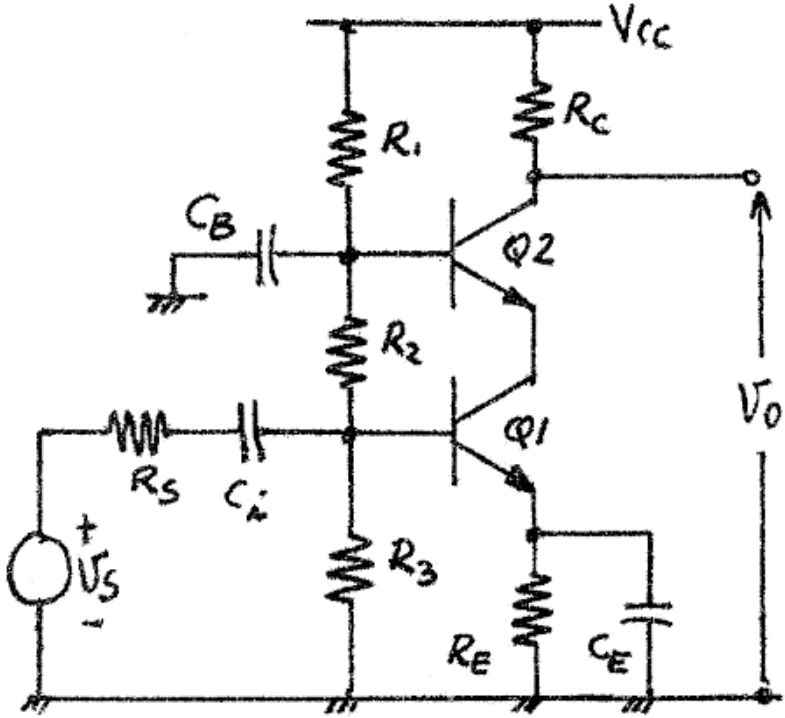
\includegraphics[width=0.5\linewidth]{_fig/multietapas_cascodo.png}
	\caption{El Cascodo}
	\label{fig:multietapas_cascodo}
\end{figure}

\begin{equation} \label{multietapas_cascodo_frecuencias-medias-equ1}
	\frac{I_o}{I_2} = \frac{\beta}{\beta +1} \approx 1 \quad \frac{I_2}{I_1} = -\beta \quad \Rightarrow \quad \frac{I_o}{I_1} \approx -\beta
\end{equation}

y

\begin{equation} \label{multietapas_cascodo_frecuencias-medias-equ2}
	\frac{V_o}{V_i} = \frac{I_o R_C}{I_i r_{\Pi}} = -\beta \frac{R_C}{r_{\Pi}} = -g_m R_C
\end{equation}

\begin{figure}[h]
	\centering
	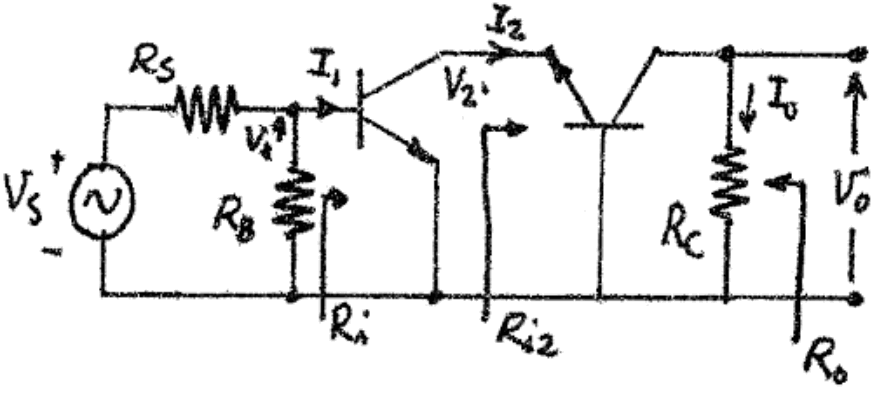
\includegraphics[width=0.5\linewidth]{_fig/multietapas_cascodo_frecuencias-medias.png}
	\caption{El Cascodo, frecuencias medias}
	\label{fig:multietapas_cascodo_frecuencias-medias}
\end{figure}

Además, $R_i = r_{\Pi}$ y $R_o = R_C$. En comparación con una configuración emisor común, se observa que la configuración cascode tiene las mismas expresiones para las ganancias de voltaje y corriente, y las resistencias de entrada y salida.

Determinación de $w_{gB}$: $C_j$ y $C_B$ tendrán expresiones para sus polos que se consiguieron en la configuración Emisor Común. En la Figura \ref{fig:multietapas_cascodo_hallar-wcb} se muestra el circuito apto para hallar el polo debido a $C_B$.

\begin{figure}[h]
	\centering
	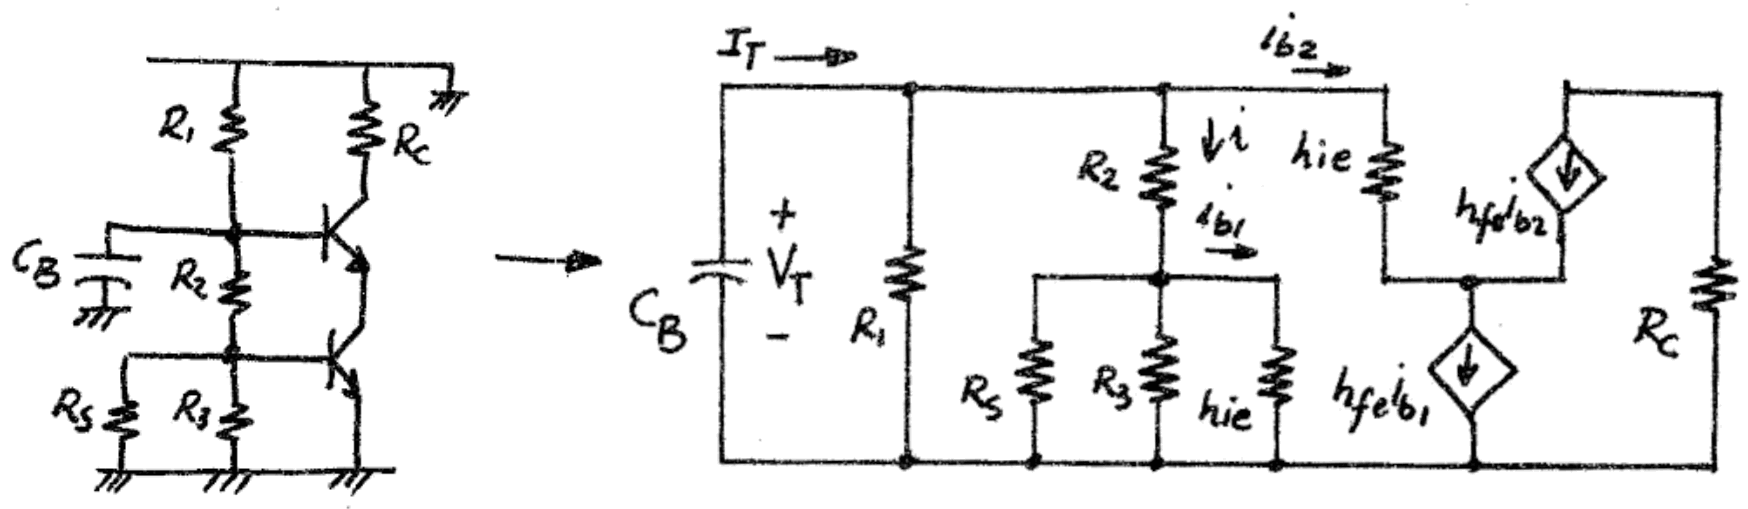
\includegraphics[width=0.8\linewidth]{_fig/multietapas_cascodo_hallar-wcb.png}
	\caption{Circuito para hallar $w_{CB}$}
	\label{fig:multietapas_cascodo_hallar-wcb}
\end{figure}

De él se desarrolla lo siguiente:

\[
I_T = \frac{V_T}{R_1} + \frac{V_T}{R_2 + R_3 \parallel R_s \parallel h_{ie}} + i_{b2}
\]

\[
i_{b1} = \frac{R_s \parallel R_3}{R_s \parallel R_3 + h_{ie}} i = \frac{R_s \parallel R_3}{R_s \parallel R_3 + h_{ie}} \cdot \frac{V_T}{R_2 + R_s \parallel R_3 \parallel h_{ie}}
\]

\[
i_{b2} = \frac{h_{fe1}}{h_{fe2} +1} i_{b1} = \frac{h_{fe1}}{h_{fe2} +1} \cdot \frac{R_s \parallel R_3}{R_s \parallel R_3 + h_{ie}} \cdot \frac{V_T}{R_2 + R_s \parallel R_3 \parallel h_{ie}}
\]

\[
R_{Th} = \frac{V_T}{I_T} = \frac{1}{\frac{1}{R_1} + \frac{1}{R_2 + \beta_3 h_{fe} h_{ie}} (1+ \frac{h_{fe}}{h_{fe} +1} \frac{R_s \parallel R_3}{R_s \parallel R_3 + h_{ie}})}
\]

Después:

\[
w_B = w_{Ci} + w_{CE} + w_{CB}
\]

Para altas frecuencias, los condensadores $C_i$, $C_E$ y $C_B$ se consideran cortocircuitos y se plantea el circuito equivalente, en donde se utiliza el modelo híbrido para los transistores, como se muestra en la Figura \ref{fig:multietapas_cascodo_frecuencias-altas}.

\begin{figure}[h]
	\centering
	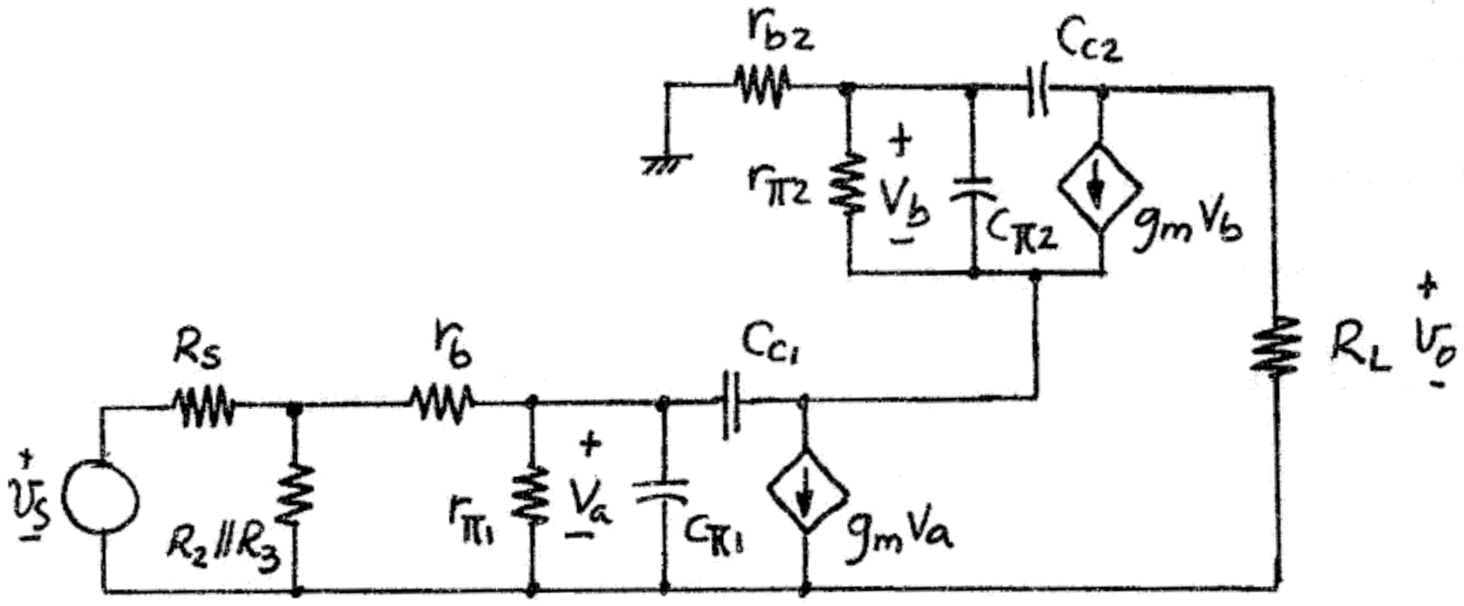
\includegraphics[width=0.8\linewidth]{_fig/multietapas_cascodo_frecuencias-altas.png}
	\caption{Modelo del Cascode para Altas Frecuencias}
	\label{fig:multietapas_cascodo_frecuencias-altas}
\end{figure}

Para hallar la constante de tiempo de $C_{T1}$, se reduce el circuito de la Figura \ref{fig:multietapas_cascodo_frecuencias-altas}, a lo que se ve en la Figura 2.10a.

Entonces:

\begin{equation} \label{multietapas_cascodo_constantes-de-tiempo-eq}
	\tau_{CT1} = C_{T1} \cdot (r_{\pi} \parallel r_6')
\end{equation}

Para \( C_C \) queda:

\begin{equation} \label{multietapas_cascodo_constantes-de-tiempo-eq-cc}
	\tau_{CC1} = C_{C1} \left[ (r_{\pi} \parallel r_6') + R_1 + g_m R_L (r_{\pi} \parallel r_6') \right]
\end{equation}

\begin{figure}[h]
	\centering
	\subfloat[Para \( C_{\pi 1} \)]
	{
		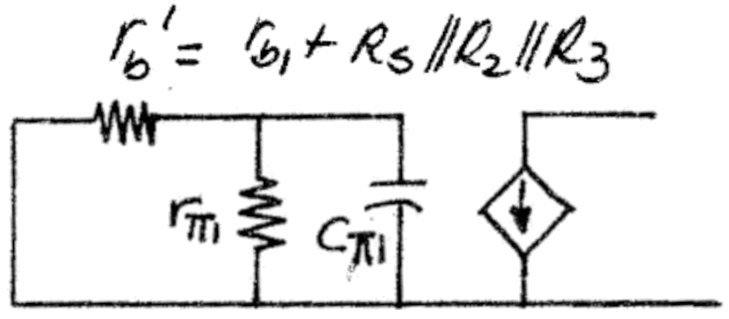
\includegraphics[width=0.32\linewidth]{_fig/multietapas_cascodo_constantes-de-tiempo-a.png}
		\label{fig:multietapas_cascodo_constantes-de-tiempo-a}
	}
	\subfloat[]
	{
		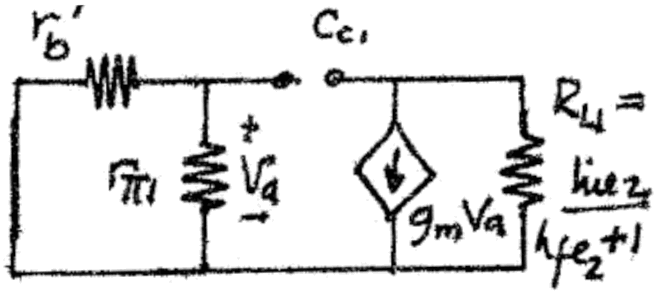
\includegraphics[width=0.32\linewidth]{_fig/multietapas_cascodo_constantes-de-tiempo-b.png}
		\label{fig:multietapas_cascodo_constantes-de-tiempo-b}
	}
	\subfloat[]
	{
		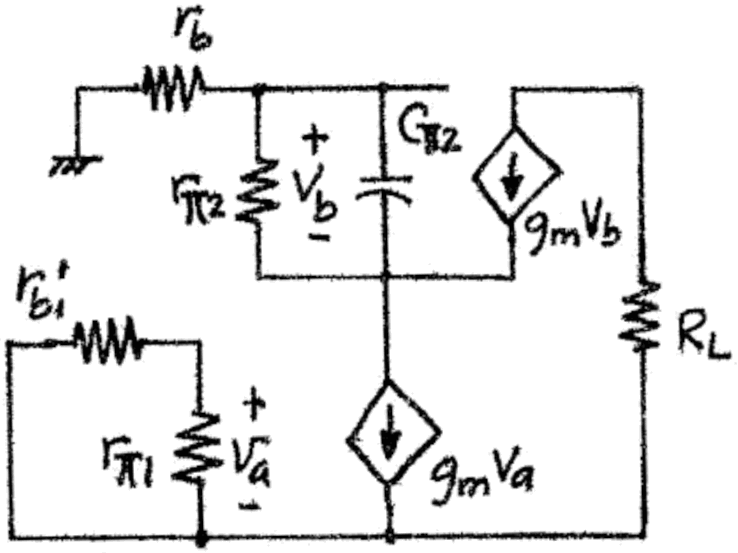
\includegraphics[width=0.32\linewidth]{_fig/multietapas_cascodo_constantes-de-tiempo-c.png}
		\label{figmultietapas_cascodo_constantes-de-tiempo-c}
	}
	\subfloat[]
	{
		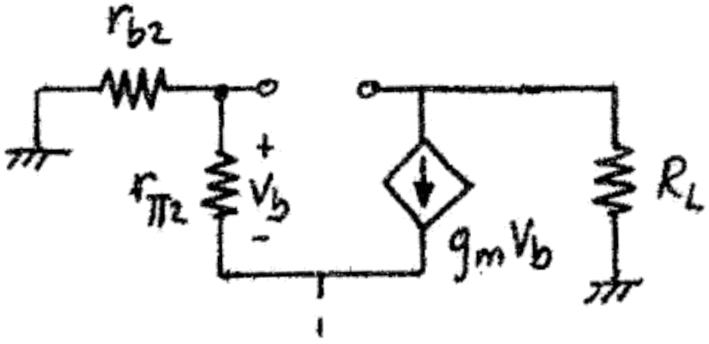
\includegraphics[width=0.32\linewidth]{_fig/multietapas_cascodo_constantes-de-tiempo-d.png}
		\label{fig:multietapas_cascodo_constantes-de-tiempo-d}
	}
	\caption{Circuitos para hallar las constantes de tiempo}
	\label{fig:multietapas_cascodo_constantes-de-tiempo}
\end{figure}

donde \( R_{L1} \) es la resistencia de carga de \( Q_1 \), es decir, la \( R_i \) de entrada de \( Q_2 \), \( R_{L1} = \frac{r_{\pi 2}}{\beta + 1} \)

Para \( C_{\pi 2} \), se hace notar que \( V_a = 0 \), con lo que se elimina el circuito de abajo.

Luego:

\[
I_T = \frac{V_T}{r_{\pi 2}} + g_{m2} V_b = V_T \left(\frac{1}{r_{\pi 2}} + g_{m2} \right)
\]

\[
R_T = \frac{r_{\pi 2}}{(1 + g_{m2} r_{\pi 2})} = \frac{r_{\pi 2}}{(\beta + 1)}
\]

\begin{equation} \label{multietapas_cascodo_eq1}
	\tau_{C\pi 2} = C_{\pi 2} \cdot \frac{r_{\pi 2}}{(\beta + 1)}
\end{equation}

Para \( C_{c2} \), se observa que en el nodo emisor de \( Q_2 \) puede plantearse así:

\[
\frac{V_b}{r_{\pi}} + g_m V_b = 0
\]

De donde concluimos que \( V_b = 0 \), y no circula corriente por esas ramas.

Entonces:

\begin{equation} \label{multietapas_cascodo_eq2}
	R_{Th} = r_{b2} + R_L, \quad \tau_{Cc2} = C_{c2} (r_{b2} + R_L)
\end{equation}

Luego, la frecuencia de corte alta viene dada por:

\[
\omega_H \approx \frac{1}{(C_{\pi 1} + C_{cc1} + \tau_{C\pi 2} + \tau_{Cc2})}
\]

\subsection{Ejemplo 2}
En el circuito de la Figura 2.11 se han polarizado ambos transistores con el mismo punto de operación: \( I_C = 2.1 mA \), \( V_{CE} = 4.5 V \). De donde: \( g_m = 0.081 \), \( \beta = 132 \), \( r_b = 60\), \( r_{\pi} = 1640 \), \( C_c = 2.2 pF \), \( C_{\pi} = 48 pF \).

\begin{figure}[h]
	\centering
	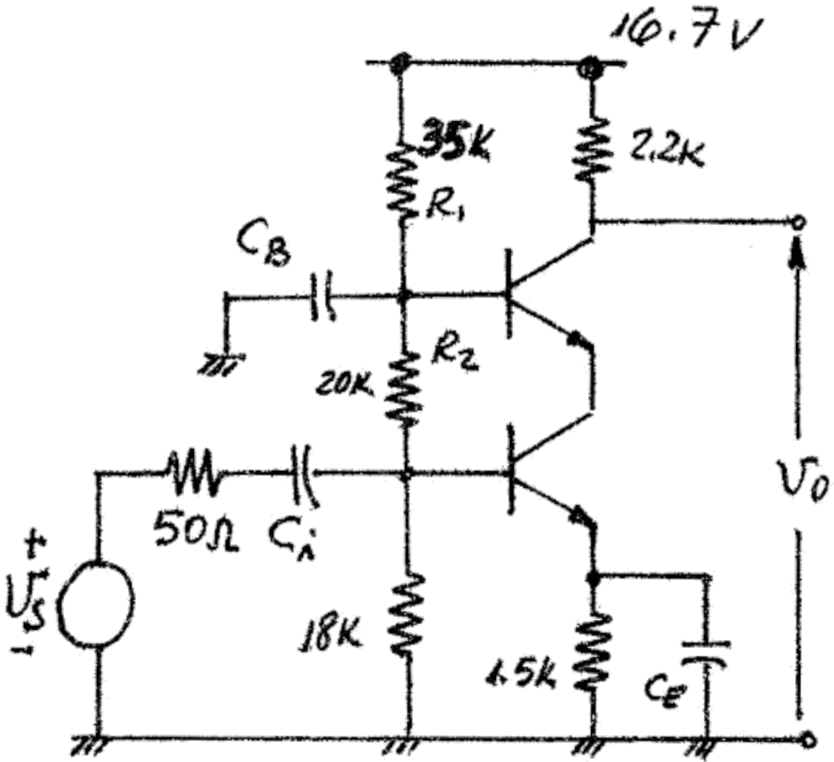
\includegraphics[width=0.8\linewidth]{_fig/multietapas_cascodo_ejemplo.png}
	\caption{Circuito de Ejemplo}
	\label{fig:multietapas_cascodo_ejemplo}
\end{figure}

Entonces, de la ecuación \ref{multietapas_cascodo_constantes-de-tiempo-eq}:

\[
\tau_{C\pi 1} = 48 \times 10^{-12} \left( 1640 \parallel ((60 + 20K) \parallel 18K \parallel 50) \right)
\]

\[
\tau_{C\pi 1} = 4.94 \times 10^{-9}
\]

de la ecuación \ref{multietapas_cascodo_constantes-de-tiempo-eq-cc}

\[
\tau_{Cc1} = 2.2 \times 10^{-12} \left(103 + \frac{1700}{133} + 0.081 \times 103 \times 1700 \right)
\]

\[
\tau_{Cc1} = 0.235 \times 10^{-9}
\]

De la ecuación \ref{multietapas_cascodo_eq1}:

\[
\tau_{C\pi 2} = 48 \times 10^{-12} \left( \frac{1640}{133} \right) = 0.68 \times 10^{-9}
\]

De la ecuación \ref{multietapas_cascodo_eq2}:

\[
\tau_{Cc2} = 2.2 \times 10^{-12} \left( 60 + 2200 \right) = 4.97 \times 10^{-9}
\]

Luego:

\[
\sum \tau = (4.94 + 0.23 + 0.68 + 4.97) \times 10^{-9} = 10.7 \times 10^{-9}
\]

y 

\[
\omega_H = \frac{1}{2\sum \tau} = \frac{1}{10.7 \times 10^{-9}} = 93.1 \times 10^6 rad/s
\]

\[
f_H = 14.8 MHz
\]

Esta cifra se puede comparar con el resultado del Ejemplo \ref{respfreq_ejm6} de un circuito emisor común con la misma ganancia, y se nota que se ha aumentado la frecuencia de corte alta por un factor de aproximadamente \( 7 \).

Además, en el circuito emisor común, se calcula el valor de la capacitancia de entrada, como:

\[
C_{entcascodo} = C_{\pi} + (1 + g_m R_L) C_c = 48 + (1 + 0.081 \times 2.2K) 2.2 = 442 pF
\]

En cambio, con los mismos datos para la configuración cascode, el valor de la capacitancia de entrada viene dado por:

\[
C_{entcascodo} = C_{\pi} + \left( 1 + g_m \frac{r_{\pi}}{\beta + 1} \right) C_{c2}
\]

\[
C_{entcascodo} = 48 + \left( 1 + 0.081 \times \frac{1700}{133} \right) 2.2 = 52.5 pF
\]

Es decir, se ha reducido la capacitancia de entrada por un factor de \( 12 \).

Finalmente, se hace notar que por medio del Método de Superposición, se puede determinar cuál de las constantes de tiempo es la más dominante, y por lo tanto la que se tiene que reducir primero si se quiere aumentar la frecuencia de corte alta.

\section{Acoplamiento directo de circuitos} %p79

Con los métodos sencillos dados, se puede analizar una configuración a fin de conseguir la frecuencia de corte deseada de alta o de baja. Para aumentar la frecuencia de corte alta, se hace necesario reducir el valor de las constantes de tiempo. Para disminuir la frecuencia de corte baja, se procura reducir el valor de los polos de los condensadores, lo cual se consigue directamente al aumentar el valor de los condensadores. Sin embargo, esta puede ser una medida costosa ya que los condensadores de valor mayor de $1 \mu F$, tienen un costo proporcional a su capacitancia y a su voltaje máximo.

Una alternativa para reducir la frecuencia de corte baja consiste en eliminar condensadores; por ejemplo, si se acopla dos etapas directamente se elimina el condensador de acople. El diseño de circuitos electrónicos sin condensadores es de interés particular para los circuitos integrados ya que las capacitancias que se pueden crear con esta técnica son muy pequeñas y ocupan mucho espacio.

Se comenzará a plantear las consideraciones a tomar en cuenta para eliminar condensadores con el ejemplo de una cascada de etapas emisor común.

\begin{figure}[h]
	\centering
	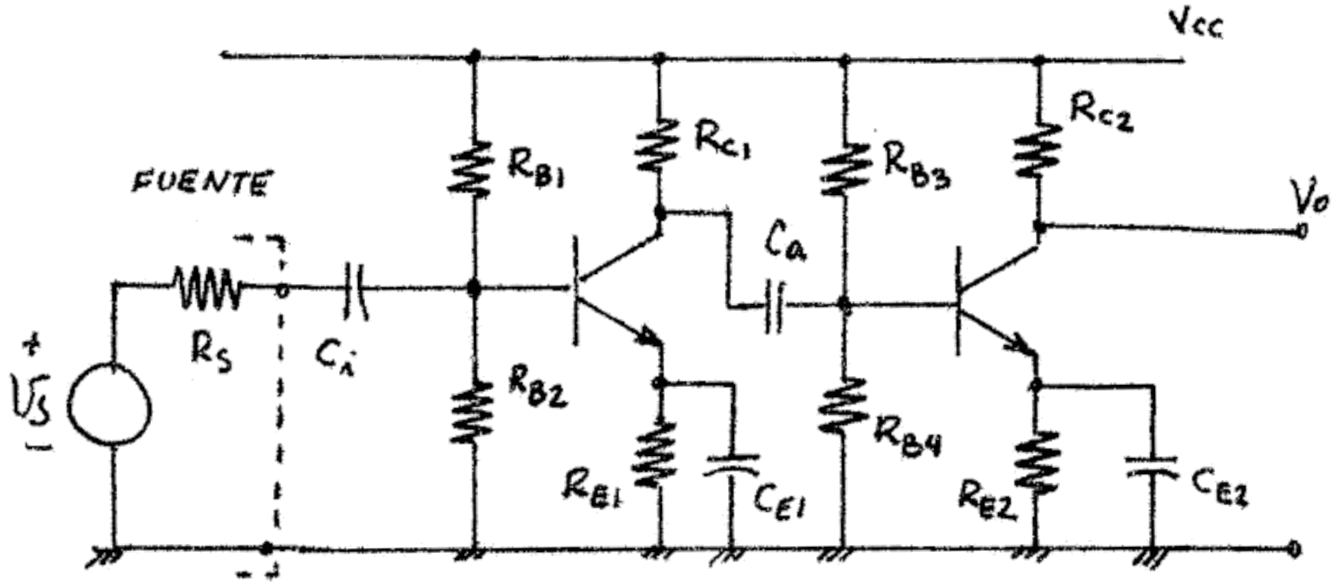
\includegraphics[width=0.8\linewidth]{_fig/multietapas_cascada-etapa-ec.png}
	\caption{Cascada de etapas EC}
	\label{fig:multietapas_cascada-etapa-ec}
\end{figure}

En la Figura \ref{fig:multietapas_cascada-etapa-ec}, se puede eliminar a $C_A$, y de paso a $R_{B3}$ y $R_{B4}$, para llegar a la configuración de la Figura \ref{fig:multietapas_cascada-etapa-ec-sin-ca}.

\begin{figure}[h]
	\centering
	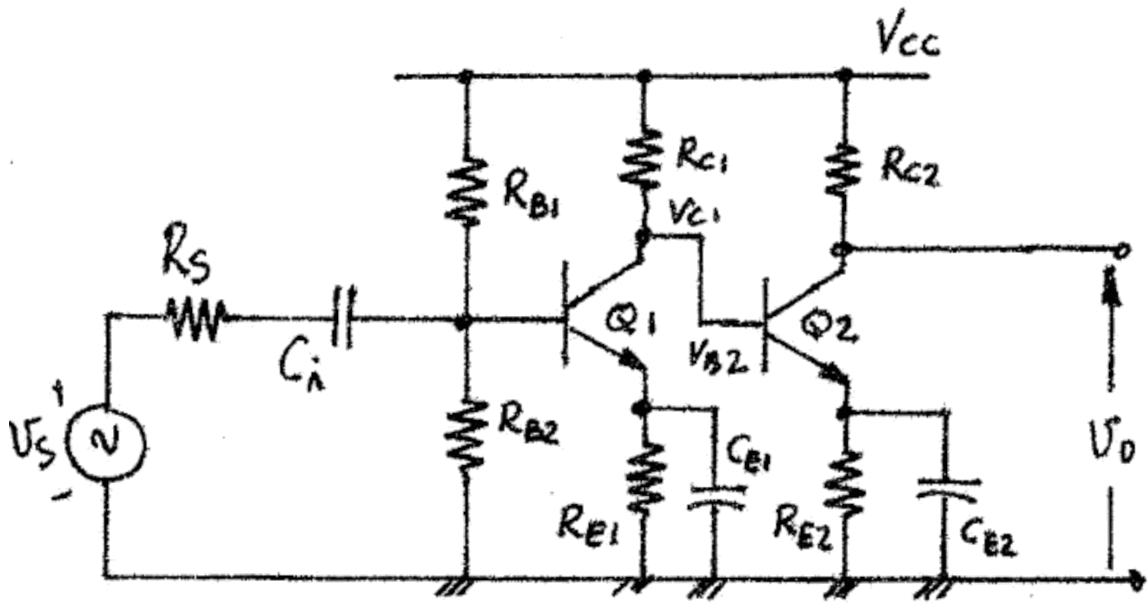
\includegraphics[width=0.8\linewidth]{_fig/multietapas_cascada-etapa-ec-sin-ca.png}
	\caption{Cascada de etapas EC sin \( C_a \)}
	\label{fig:multietapas_cascada-etapa-ec-sin-ca}
\end{figure}

Se puede conectar el colector de $Q_1$ directamente a la base de $Q_2$ cuando el nivel de continua en estas dos puntos es el mismo.

\begin{figure}[h]
	\centering
	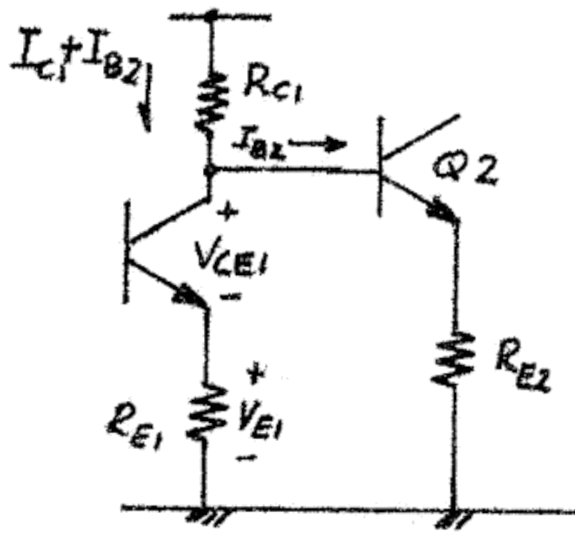
\includegraphics[width=0.8\linewidth]{_fig/multietapas_cascada-etapa-ec_pol-segunda-etapa.png}
	\caption{Cascada EC, polarización segunda etapa}
	\label{fig:multietapas_cascada-etapa-ec_pol-segunda-etapa}
\end{figure}

Para este circuito, la polarización de la primera etapa queda igual. El circuito de polarización de la segunda etapa se muestra en la Figura \ref{fig:multietapas_cascada-etapa-ec_pol-segunda-etapa}. La corriente que pasa por $R_{C1}$ es $I_{C1} + I_{B2}$, $R_{E2}$ puede ser escogida para que se cumpla la condición necesaria de \( V_{C1} = V_{B2} \); se hace notar que la polarización de la segunda etapa está íntimamente relacionada con la polarización de la primera etapa. Es decir, queda:

\[
R_{E2} = \frac{V_{CC} - (I_{C1} + I_{B2})R_{C1} - V_{BE2}}{(\beta +1) I_{B2}}
\]

La misma idea se aplica a fin de eliminar $C_i$ a la entrada del amplificador; para acoplar la fuente directamente al amplificador tiene que existir el mismo nivel de continua en los puntos a conectar. En el caso general, la fuente de entrada tiene un nivel de continua igual a cero, por lo que se modifica el amplificador a fin de que también tenga un nivel de continua igual a cero en su entrada.

Se logra llevar la entrada a cero volt, y a la vez polarizar la junta BE del transistor de entrada, al utilizar una fuente de poder bipolar (positiva y negativa), como se muestra en la Figura \ref{fig:multietapas_cascada-etapa-ec_fuente-bipolar}.

\begin{figure}[h]
	\centering
	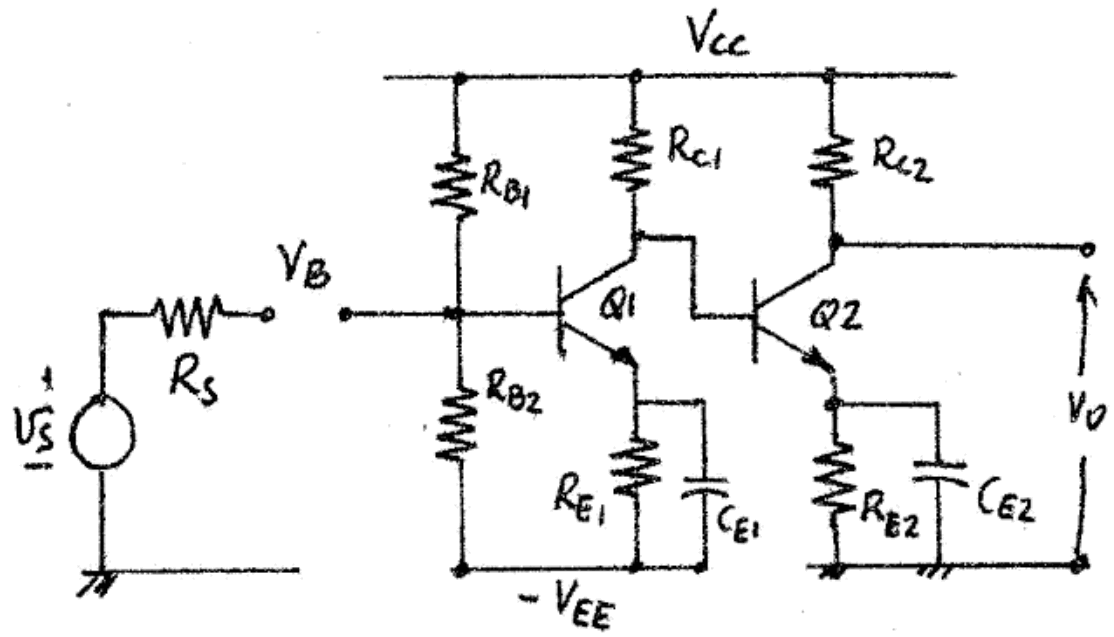
\includegraphics[width=0.8\linewidth]{_fig/multietapas_cascada-etapa-ec_fuente-bipolar.png}
	\caption{Cascada EC, con fuente bipolar}
	\label{fig:multietapas_cascada-etapa-ec_fuente-bipolar}
\end{figure}

Se ajusta los valores de $R_{B1}$ y $R_{B2}$ de modo que el nivel continuo de $V_B$ sea igual a 0. También se podría eliminar $R_{B1}$ y $R_{B2}$, y en tal caso, la corriente de base de polarización es suministrada por la fuente de entrada. Esto crea un pequeño nivel negativo $= -I_B R_S$, a la entrada del amplificador. Vea la Figura \ref{fig:multietapas_cascada-etapa-ec_sin-rb}.

\begin{figure}[h]
	\centering
	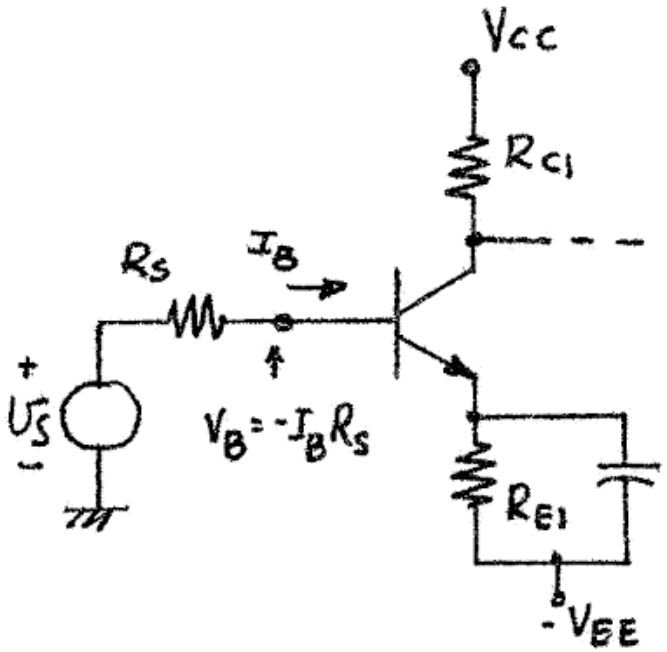
\includegraphics[width=0.8\linewidth]{_fig/multietapas_cascada-etapa-ec_sin-rb.png}
	\caption{Cascada EC, entrada sin \( R_B \)}
	\label{fig:multietapas_cascada-etapa-ec_sin-rb}
\end{figure}

Dado nuestro objetivo de un amplificador sin condensadores, aún nos quedan los de puenteo de emisor, $C_{E1}$ y $C_{E2}$ en la Figura \ref{fig:multietapas_cascada-etapa-ec_fuente-bipolar}. Veamos $C_E$ y $R_E$: $R_E$ le imprime una estabilidad térmica a la etapa, y a su vez, $C_E$ la puentea a frecuencias medias a fin de aumentar la ganancia del circuito. En la Figura \ref{fig:multietapas_amp-fuente-continua}, se plantean dos amplificadores de corriente continua. El de la Figura \ref{fig:multietapas_amp-fuente-continua_buena-ganancia} tiene buena ganancia pero mala estabilidad térmica. El de la Figura \ref{fig:multietapas_amp-fuente-continua_buena-estabilidad} tiene buena estabilidad térmica pero poca ganancia.

\begin{figure}[h]
	\centering
	\subfloat[Buena Ganancia]
	{
		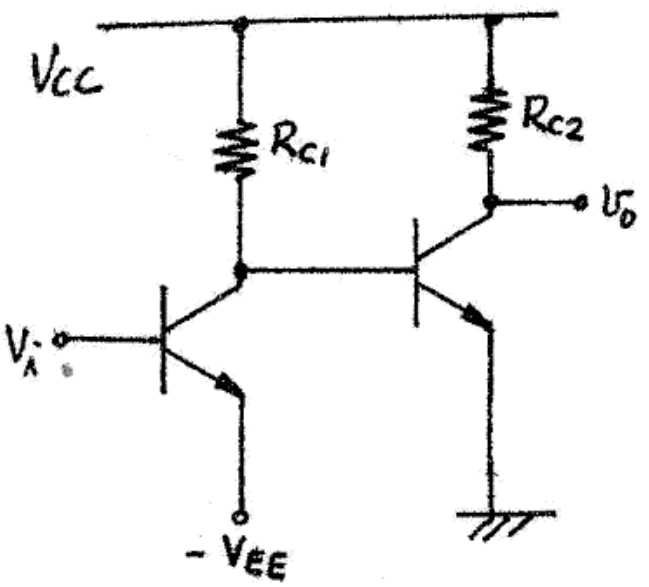
\includegraphics[width=0.46\linewidth]{_fig/multietapas_amp-fuente-continua_buena-ganancia.png}
		\label{fig:multietapas_amp-fuente-continua_buena-ganancia}
	}
	\subfloat[Buena Estabilidad Térmica]
	{
		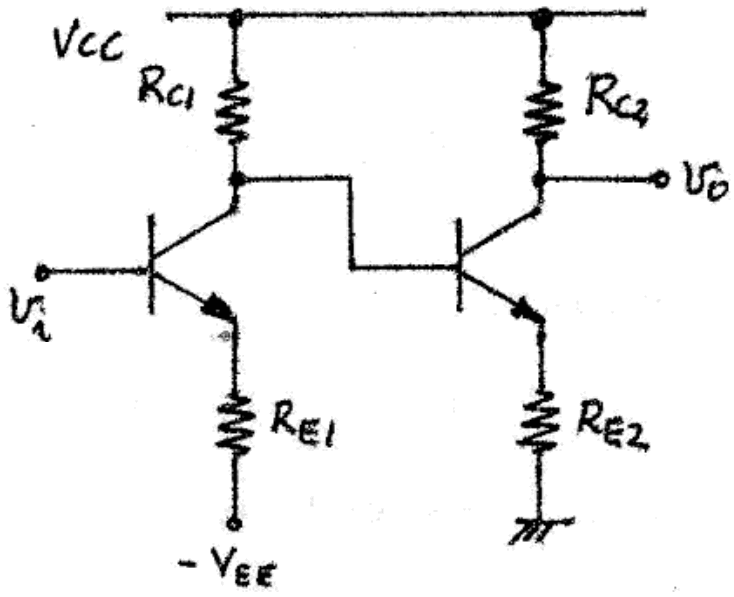
\includegraphics[width=0.46\linewidth]{_fig/multietapas_amp-fuente-continua_buena-estabilidad.png}
		\label{fig:multietapas_amp-fuente-continua_buena-estabilidad}
	}
	\caption{Amplificadores de corriente continua}
	\label{fig:multietapas_amp-fuente-continua}
\end{figure}

\section{La configuracion diferencial} %p83

La configuración que logra combinar una ganancia buena con una estabilidad térmica excelente es la configuración diferencial de la Figura \ref{fig:multietapas_conf-diferencial}. La resistencia de emisor es la que le proporciona su buena estabilidad térmica. A su vez, la cascada de transistores le proporciona una buena ganancia.

Antes de analizar en detalle esta configuración, vamos a presentar algunas características de la configuración diferencial general. Se hace notar que hay dos entradas y una salida sencilla, que se representa esquemáticamente en la Figura \ref{fig:multietapas_esquema-sistema-diferencial}. La diferencia entre las entradas se llama la entrada diferencial, $V_d$, donde:

\begin{equation}
	V_d = V_1 - V_2
\end{equation}

\begin{figure}[h]
	\centering
	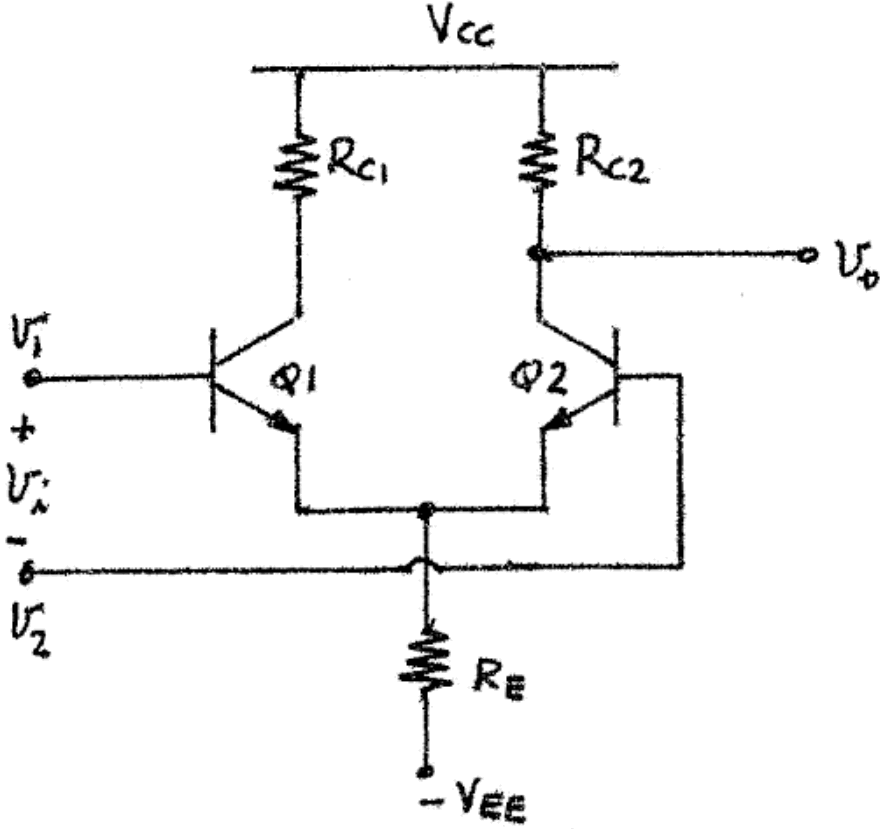
\includegraphics[width=0.6\linewidth]{_fig/multietapas_conf-diferencial.png}
	\caption{La configuración diferencial}
	\label{fig:multietapas_conf-diferencial}
\end{figure}

\begin{figure}[h]
	\centering
	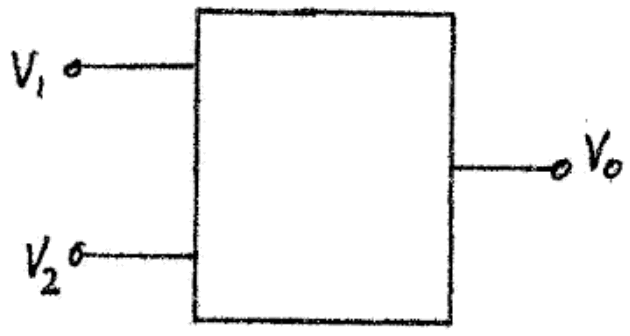
\includegraphics[width=0.4\linewidth]{_fig/multietapas_esquema-sistema-diferencial.png}
	\caption{Esquema de sistema diferencial}
	\label{fig:multietapas_esquema-sistema-diferencial}
\end{figure}

A su vez, las entradas tienen un componente común, que viene dado por el valor promedio de las entradas,

\begin{equation}
	V_c = (V_1 + V_2)/2
\end{equation}

Se tiene:

\begin{equation}
	V_o = A_1 V_1 + A_2 V_2
\end{equation}

donde

\begin{equation}
	A_1 = \frac{V_o}{V_1} \quad \text{con } V_2 = 0
\end{equation}

\begin{equation}
	A_2 = \frac{V_o}{V_2} \quad \text{con } V_1 = 0
\end{equation}

Alternativamente, podemos expresar a $V_o$ en función de la señal diferencial de entrada, y la componente común. Entonces:

\begin{equation}
	V_o = A_d V_d + A_c V_c
\end{equation}

Si se expresan las señales $V_1$ y $V_1$ en función de las señales $V_d$ y $V_c$ se obtiene:

\begin{equation}
	V_1 = V_c + \frac{V_d}{2}
\end{equation}

\begin{equation}
	V_2 = V_c - \frac{V_d}{2}
\end{equation}

Se puede relacionar las ganancias $A_1$ y $A_2$ con las ganancias de $A_d$ y $A_c$ y se obtiene:

\begin{equation} \label{multietapas_conf-diff_ac}
	A_c = A1 + A2
\end{equation}

\begin{equation} \label{multietapas_conf-diff_ad}
	A_d = \frac{A1 + A2}{2}
\end{equation}

\subsection{Ejemplo 3}

\textbf{Demuestre las relaciones de las Ecuaciones \ref{multietapas_conf-diff_ac} y \ref{multietapas_conf-diff_ad}.}

En los llamados Amplificadores Diferenciales se busca resaltar la ganancia diferencial frente a la ganancia de modo común. Un criterio de calidad para un amplificador5 diferencial es la relación entre la ganancia de modo diferencial y la de modo común, conocida como la relación de rechazo de modo común, que generalmente se expresa en $dB$.

\begin{equation}
	\text{CMRR} = 20 log | \frac{A_d}{A_c} | 
\end{equation}

Frecuentemente, los amplificadores diferenciales están diseñados para servir como amplificadores de corriente continua. El nivel de continua que se puede aplicar simultaneamente a ambas entradas está limitado y se conoce como el \textbf{Rango de Modo Común}. Si se aplica un nivel común fuera de éste rango, el circuito deja de trabajar como amplificador lineal, y eventualmente se puede dañar.

\subsection{Circuito simétrico con salida sencilla entrada diferencial} %p85

Vamos a analizar al circuito diferencial con el cual comenzamos esta sección, la Figura \ref{fig:multietapas_conf-diferencial}. Encontraremos las relaciones salida/entrada de dos modos: por medio del modelo de pequeña señal, y utilizando el Teorema de Bisección que describiremos después.

Más adelante veremos que la configuración diferencial tiene tanto una zona lineal de operación como una zona no lineal. En la Figura \ref{fig:multietapas_superposicion-ac_conf-diferencial} se plantea el modelo de pequeña señal y al mismo tiempo se aplica el Teorema de Superposición para encontrar la salida \( V_o \) en función de las dos entradas \( V_1 \) y \( V_2 \), es decir, 

\[
A_1 = \frac{V_o}{V_1}, \quad A_2 = \frac{V_o}{V_2}.
\]

El Teorema de Superposición es aplicable solo si el circuito trabaja en forma lineal.

\begin{figure}[h]
	\centering
	\subfloat[Para hallar \( A_1 \)]
	{
		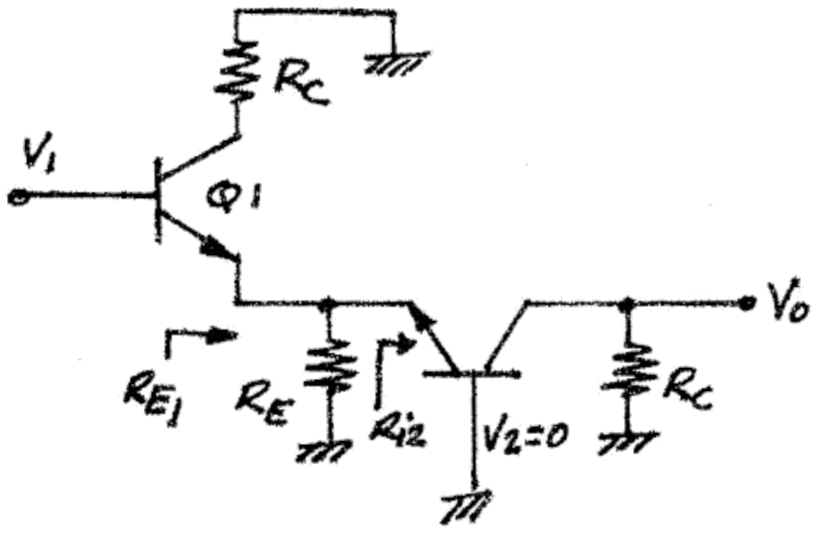
\includegraphics[width=0.46\linewidth]{_fig/multietapas_superposicion-ac_conf-diferencial-a1.png}
		\label{fig:multietapas_superposicion-ac_conf-diferencial-a1}
	}
	\subfloat[Para hallar \( A_2 \)]
	{
		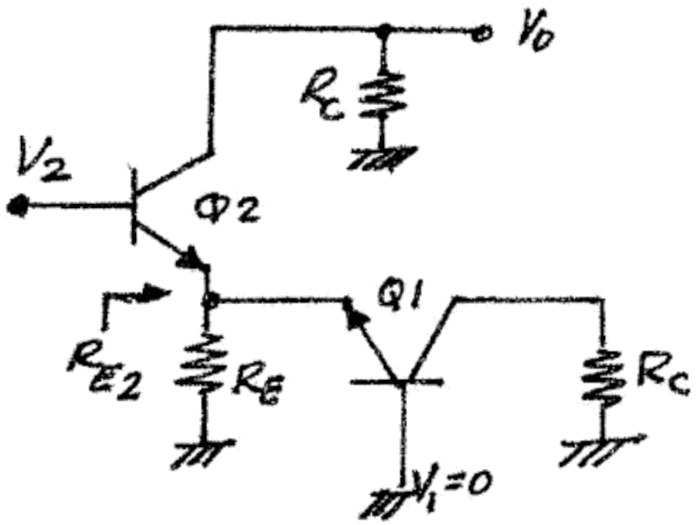
\includegraphics[width=0.46\linewidth]{_fig/multietapas_superposicion-ac_conf-diferencial-a2.png}
		\label{fig:multietapas_superposicion-ac_conf-diferencial-a2}
	}
	\caption{Teorema de Superposición aplicado en AC a la Configuración Diferencial}
	\label{fig:multietapas_superposicion-ac_conf-diferencial}
\end{figure}

En la Figura \ref{fig:multietapas_superposicion-ac_conf-diferencial-a1}, \( \frac{V_o}{V_1} = \frac{V_o}{V_a} \times \frac{V_a}{V_1}\), la cascada de un amplificador colector común \( Q1 \) con un amplificador base común \( Q2\).

La ganancia del amplificador base común \( Q2 \) es: \( \frac{V_o}{V_a} = g_m R_C \).

La ganancia del amplificador colector común \( Q1 \) es: \( \frac{V_a}{V_1} = \frac{(\beta+1) R_{EI}}{r_\pi + (\beta+1) R_{EI}} \)

donde: \( R_{EI} = R_E \parallel \frac{r_\pi}{\beta+1} \)

o, \( \frac{V_a}{V_1} = \frac{(\beta+1) R_{EI}}{2 (\beta+1) R_E + r_\pi} = \frac{1}{2 + \frac{r_\pi}{(\beta+1) R_E}} \)

y,

\begin{equation} \label{multietapas_ac_conf-diff_a1}
	A_1 = \frac{V_o}{V_1} = \frac{g_m R_L}{2 + \frac{r_\pi}{(\beta+1) R_E}} \approx \frac{g_m R_L}{2}
\end{equation}

es decir, la ganancia del conjunto como amplificador sencillo (salida sencilla, entrada sencilla) es aproximadamente la mitad de la ganancia de la configuración emisor común, pero sigue siendo una ganancia bastante elevada.

Por el otro lado, de la Figura \ref{fig:multietapas_superposicion-ac_conf-diferencial-a2}, se tiene

\( A_2 = \frac{V_o}{V_2} = \frac{-\beta R_L}{r_\pi + (\beta+1) R_{E2}} \), donde  \( R_{E2} = R_E \parallel \frac{r_\pi}{(\beta+1)} \)

\begin{equation} \label{multietapas_ac_conf-diff_a2}
	A_2 = - g_m R_L \left[ \frac{(\beta+1) R_E + r_\pi}{2 (\beta+1) R_E + r_\pi} \right]
\end{equation}

Si se comparan \( A_1 \) y \( A_2 \) en las ecuaciones \ref{multietapas_ac_conf-diff_a1} y \ref{multietapas_ac_conf-diff_a2} se nota que son casi iguales excepto por el signo. Con \( A_1 \) y \( A_2 \) se pueden obtener las ganancias diferenciales y de modo común, al aplicar las ecuaciones \ref{multietapas_conf-diff_ac} y \ref{multietapas_conf-diff_ad}:

\begin{equation}
	A_d = \frac{A_1 - A_2}{2} = \frac{g_m R_L \left[ 2 (\beta+1) R_E + r_\pi \right]}{2 \left[ 2 (\beta+1) R_E + r_\pi \right]} = \frac{g_m R_L}{2}
\end{equation}

\[
A_c = A_1 + A_2 = - g_m R_L \frac{r_\pi}{[2(\beta+1) R_E + r_\pi]}
\]

\begin{equation}
	A_c = \frac{- \beta R_L}{2 (\beta+1) R_E + r_\pi}
\end{equation}

Para terminar de resolver las ecuaciones anteriores hay que determinar el punto de operación del circuito. Normalmente el nivel DC en las entradas \( V_1 \) y \( V_2 \) es el mismo y en ese caso la corriente que circula por la resistencia del emisor se divide en partes iguales por los dos transistores, \( I_{C1} = I_{C2} = \frac{I_E}{2} \). La tensión en el emisor, \( V_e \), se encuentra como la tensión en las bases, menos la tensión base-emisor. Después,

\begin{equation}
	I_E = \frac{(V_e - V_{ee})}{R_E}
\end{equation}

Una vez conocidas todas las corrientes que circulan por todas las ramas, se puede determinar las tensiones en todas partes del circuito.

Una alternativa muy apropiada para analizar este circuito utiliza el Teorema de Bisección (Angelo, p.426). Es aplicable a redes que son simétricas, es decir que pueden ser divididas en dos partes iguales, cada parte con su fuente de entrada, tal como se muestra en la Figura \ref{fig:multietapas_red-teorema-biseccion}.

\begin{figure}[h]
	\centering
	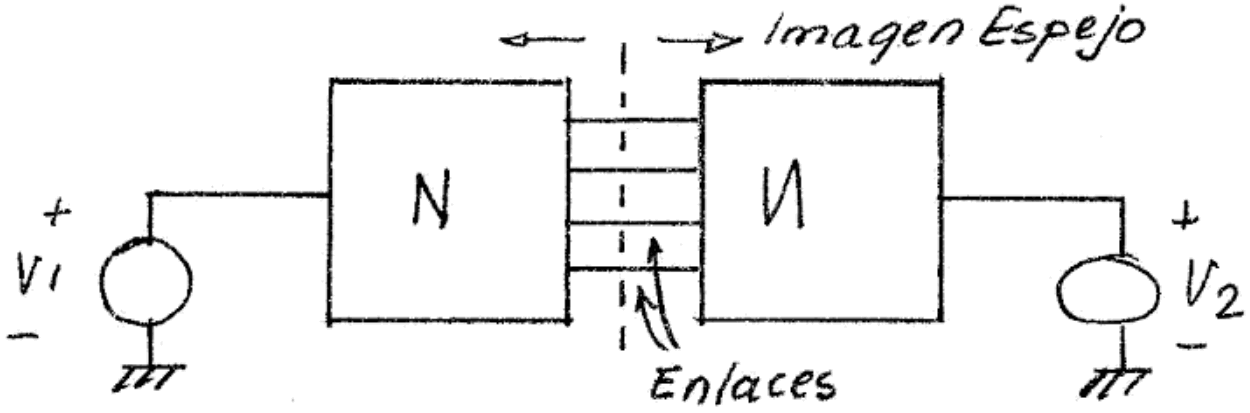
\includegraphics[width=0.8\linewidth]{_fig/multietapas_red-teorema-biseccion.png}
	\caption{Red apto para aplicar el Teorema de Bisección}
	\label{fig:multietapas_red-teorema-biseccion}
\end{figure}

El Teorema dice que cuando se aplica una señal igual o común a las dos entradas, se puede cortar los enlaces que unen las dos redes sin por eso modificar las tensiones y corrientes. En el caso de aplicar señales opuestas, la señal diferencial, se cortocircuitan los enlaces que unen los dos circuitos y se considera que se aplica una señal de valor $V_d / 2$, y de esta manera se pueden obtener las relaciones que corresponden a este caso. Esquemáticamente se representa en la Figura \ref{fig:multietapas_teorema-biseccion}.

\begin{figure}[h]
	\centering
	\subfloat[Modo Común]
	{
		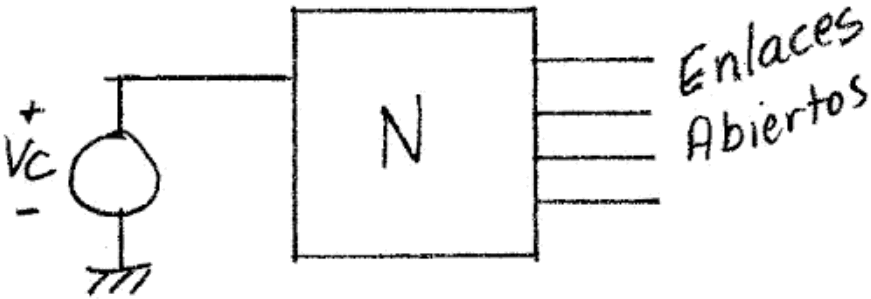
\includegraphics[width=0.46\linewidth]{_fig/multietapas_teorema-biseccion_modo-comun.png}
		\label{fig:multietapas_teorema-biseccion_modo-comun}
	}
	\subfloat[Modo Diferencial]
	{
		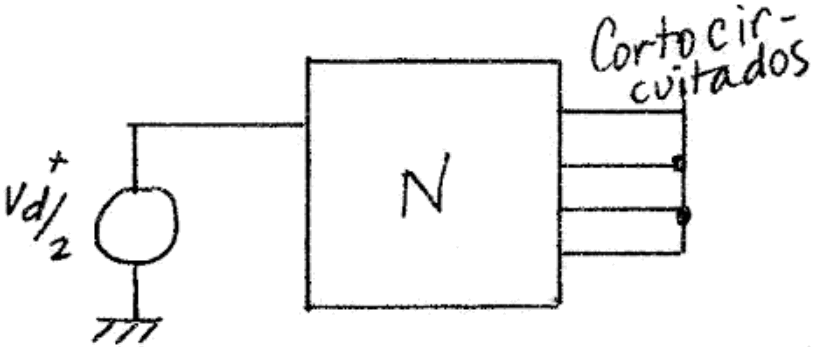
\includegraphics[width=0.46\linewidth]{_fig/multietapas_teorema-biseccion_modo-diferencial.png}
		\label{fig:multietapas_teorema-biseccion_modo-diferencial}
	}
	\caption{Aplicación de Teorema de Bisección}
	\label{fig:multietapas_teorema-biseccion}
\end{figure}

Para efectos de determinar el punto de operación y la ganancia de modo común, $A_c$, se aplica una excitación simétrica a la Figura \ref{fig:multietapas_conf-diferencial}, $V_1 = V_2 = V_c$, y resulta el equivalente de la Figura \ref{fig:multietapas_sch-teorema-biseccion_modo-comun}. De aquí se consigue:

\begin{enumerate}
	\item[a)] \( A_C = \frac{-\beta R_C}{r_{\pi} + (\beta +1)2R_E} \)
	\item[b)] \( V_E = -V_{BE} + V_{EE} \approx V_{EE} - 0.7 \)
\end{enumerate}

De donde:
\[
I_E = \frac{(V_{EE} - 0.7)}{2R_E}
\]

\begin{figure}[h]
	\centering
	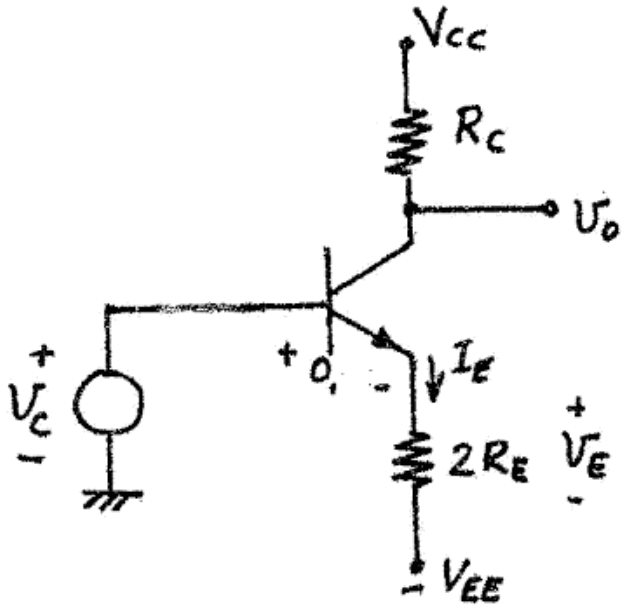
\includegraphics[width=0.6\linewidth]{_fig/multietapas_sch-teorema-biseccion_modo-comun.png}
	\caption{Teorema de Bisección, Modo común (esquema)}
	\label{fig:multietapas_sch-teorema-biseccion_modo-comun}
\end{figure}

Para hallar la ganancia y otras características de modo diferencial, se aplica una excitación antisimétrica a la Figura \ref{fig:multietapas_conf-diferencial}, \( V_1 = -V_2 = V_d/2 \), y resulta el equivalente de la Figura \ref{fig:multietapas_sch-teorema-biseccion_modo-diferencial}.

\begin{equation} \label{multietapas_ganancia-diferencial}
	A_d = \frac{-\beta R_C}{2r_{\pi}}
\end{equation}

\begin{figure}[h]
	\centering
	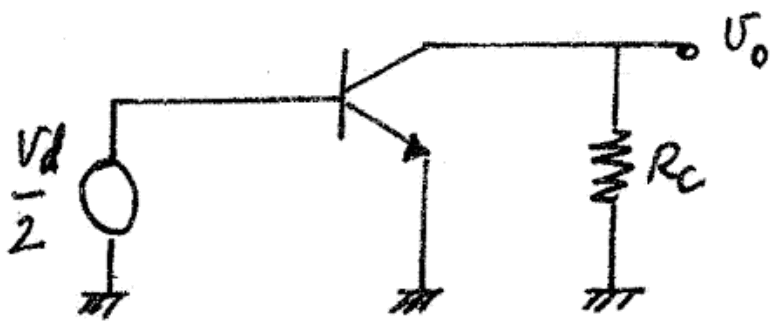
\includegraphics[width=0.8\linewidth]{_fig/multietapas_sch-teorema-biseccion_modo-diferencial.png}
	\caption{Teorema de Bisección, Modo diferencial (esquema)}
	\label{fig:multietapas_sch-teorema-biseccion_modo-diferencial}
\end{figure}

Como en el caso de la configuración EC, la resistencia \( R_E \) le proporciona estabilidad térmica al circuito, disminuyendo el cambio de \( I_C \) con cambios de temperatura; valores mayores de \( R_E \) hacen el circuito más estable. La expresión de la ganancia diferencial \ref{multietapas_ganancia-diferencial} demuestra que su valor es grande, siendo la mitad de la ganancia del EC.

El valor de la Relación de Rechazo de Modo Común para el circuito de la Figura \ref{fig:multietapas_conf-diferencial} viene dado por:

\begin{equation}
	\text{CMRR} = 20 \log \left( \frac{\beta R_L}{2(R_S + r_{\pi})} \middle/ \frac{\beta R_C}{(R_S + r_{\pi} + 2(\beta+1)R_E)} \right) 
	\approx 20 \log \left( \frac{\beta R_E}{R_S + r_{\pi}} \right)
\end{equation}

Se puede ver que la CMRR también se favorece con aumentos de \( R_E \). Sin embargo, para una \( I \) constante, cuanto más grande sea \( R_E \), más desperdicio de potencia hay debido a la caída en \( R \).

Un dispositivo que teóricamente representa una resistencia infinita, pero que tiene una caída de voltaje finita es una fuente de corriente. En la Figura \ref{fig:multietapas_fuente-corriente-transistorizada} se muestra una posible configuración. La combinación de \( R_1 \) y \( R_2 \) fija el nivel en la base del transistor. Entonces:

\[
V_3 = -V_b - V_{BE} = (-V_{EE})
\]

donde: \( V_b = R_1 V_{BE} / (R_1 + R_2) \)

Luego: \( I \equiv I_3 = \frac{V_3}{R_3} = \frac{(V_{EE} - V_b + V_{BE})}{R_3} \)

\begin{figure}[h]
	\centering
	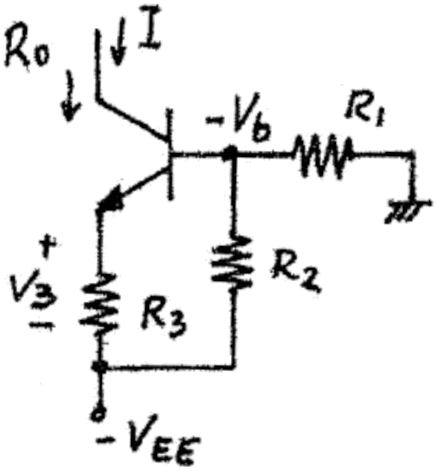
\includegraphics[width=0.4\linewidth]{_fig/multietapas_fuente-corriente-transistorizada.png}
	\caption{Fuente de Corriente Transistorizada (Reemplaza a \( R_E \) en la Figura \ref{fig:multietapas_conf-diferencial})}
	\label{fig:multietapas_fuente-corriente-transistorizada}
\end{figure}

Esta configuración se aproxima a una fuente de corriente por la impedancia alta vista desde el colector de un transistor en la región activa. La corriente que suministra es prácticamente constante y controlada por \( R_3 \). En reposo la corriente se divide en partes iguales por los transistores \( Q_1 \) y \( Q_2 \). La expresión para la resistencia de salida viene dada por (Millman-Halkias):

\begin{equation}
	R_o = \frac{(1+\beta)R_3 + R_{\phi} + r_{\pi} (1+h_{oe}R_3)}{h_{oe} (R_3 + R_{\phi} + r_{\pi} - h_{re} \beta / h_{oe})}, \quad R_{\phi} = R_1 \parallel R_2
\end{equation}

\subsubsection{Ejemplo 4}
Hallar el punto de operación, \( R_3 \) y la ganancia de modo diferencial del circuito de la Figura \ref{fig:multietapas_ejemplo4-sch}.

\begin{figure}[h]
	\centering
	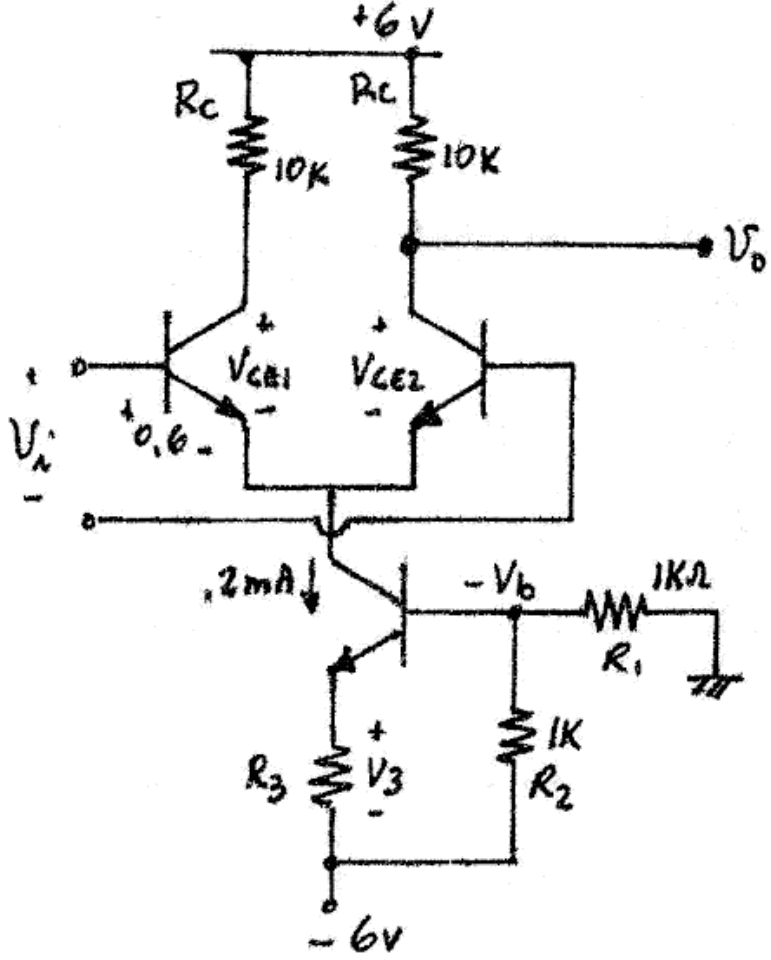
\includegraphics[width=0.7\linewidth]{_fig/multietapas_ejemplo4-sch.png}
	\caption{Circuito de Ejemplo}
	\label{fig:multietapas_ejemplo4-sch}
\end{figure}

\textbf{Solución:}

Con \( R_1 = R_2 = 1K \),

entonces: \( -V_b = \frac{-6}{2} = -3 \)

después: \( V_3 = +6 - (0.6 + 3) = +2.4V \)

y \( R_3 = \frac{V_3}{I} = \frac{2.4V}{0.2mA} = 12K\Omega \)

Entonces: \( V_{CE3} = -V_{BE1} + V_{EE} - V_3 = 3V \)

\( V_{CE1} = V_{CE2} = V_{CC} - I_C R_C - V_E = 6 - (0.1)(10K) - (-6.7) = 5.7V \)

\( g_m = \frac{I_C}{V_T} = 3.8 \times 10^{-3} \)

\( r_{\pi} = \frac{\beta}{g_m} = 26K \) (Se hace notar el valor elevado)

\( R_i = 2 r_{\pi} = 52K \)

\( A_d = \frac{+\beta R_C}{2r_{\pi}} \approx +20 \)

La junta BE de \( Q_3 \) tendrá una caída de voltaje que variará con variaciones de temperatura, que en consecuencia hará variar la corriente de la fuente. Para compensar este cambio, se puede colocar componentes en la red de polarización de base, como por ejemplo los diodos en la Figura \ref{fig:multietapas_ejemplo4_comp-termica}, con el mismo coeficiente térmico que la junta BE del transistor, de modo que no varíe la tensión en \( R_3 \), y tampoco la corriente de colector.

\begin{figure}[h]
	\centering
	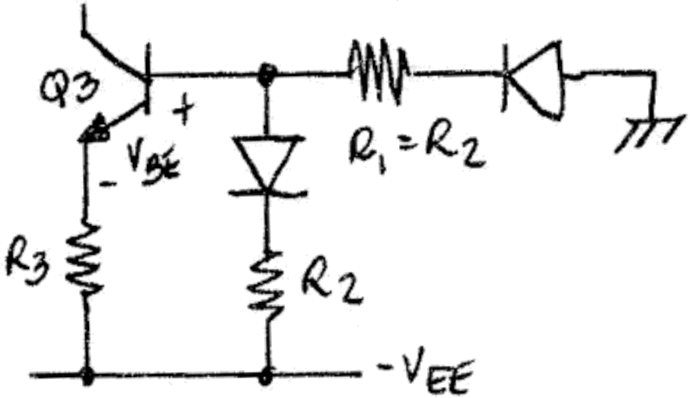
\includegraphics[width=0.6\linewidth]{_fig/multietapas_ejemplo4_comp-termica.png}
	\caption{Compensación Térmica de \( V \)}
	\label{fig:multietapas_ejemplo4_comp-termica}
\end{figure}

Encontremos ahora el \textbf{rango de modo común}. En el circuito de la Figura \ref{fig:multietapas_ejemplo4-sch}, hemos supuesto que el nivel de continua común a las entradas es 0V, y con este valor se ha obtenido \( V_{CE3} = 3V \), y \( V_{CE1} = V_{CE2} = 5.6V \). 

Si el nivel común aplicado a las entradas disminuye, se hace negativo, entonces \( V_{CE3} \) disminuye y \( V_{CE1} = V_{CE2} \) aumentan. La configuración conserva su carácter de amplificador mientras \( Q_3 \) cumple la función de una fuente de corriente, lo que exige que \( Q_3 \) permanezca en la región activa, o que:

\[
V_{CE3} > 0.2V
\]

Esto a su vez implica:

\[
V_{BI} = V_{B2} > -V_{EE} + V_3 + V_{CE3} (\text{mín}) + V_{BE}
\]

\[
V_{BI} = -6 + 3 + 0.2 + 0.7 = -2.1V
\]

Entonces, el nivel mínimo de las entradas es \( V_{BI} = V_{B2} > -2.1V \), para que \( Q_3 \) cumpla la función de fuente de corriente.

Y ¿cómo se establece el nivel máximo? A medida que aumenta \( V_{BI} = V_{B2} \), disminuye \( V_{CE1} = V_{CE2} \). Sin embargo, \( V_{CE1} \) y \( V_{CE2} \) requieren un nivel mínimo para permitir que la señal de salida pueda variar como respuesta a la señal de entrada. En el circuito de la Figura 2.27, con \( V_{BI} = V_{B2} = 0 \), entonces tenemos \( I_C = 0.1 \) mA, y \( V_{CE} = V_{CC} - I_C R_C - V_E = 6 - (0.1 \times 10) - 0.7 = 5.7V \), es decir, el punto de operación es \( (V_{CE}, I_C) = (5.7V, 0.1 \text{ mA}) \). En la Figura \ref{fig:multietapas_ejemplo4_recta-de-carga} se muestra la recta de carga. A medida que \( V_{BI} = V_{B2} \) aumenta, esta recta va desplazándose a la izquierda.

Para la mayor variación de salida se requiere que:

\[
V_{CC} - V_{EI} - I R_C > 0.2V
\]

o 

\[
V_{EI} < V_{CC} - I R_C - 0.2 = 6 - 2 - 0.2 = 3.8V
\]

Y como 

\[
V_{EI} = V_{BI} - 0.7
\]

luego 

\[
V_{BI} = V_{EI} + 0.7 > 3.8 + 0.7 = 4.5V
\]

Entonces el nivel máximo de \( V_{BI} = V_{B2} \) es 4.5V.

El Rango de Modo Común queda:

\[
-2.1V < V_{BI} = V_{B2} < 4.5V
\]

\begin{figure}[h]
	\centering
	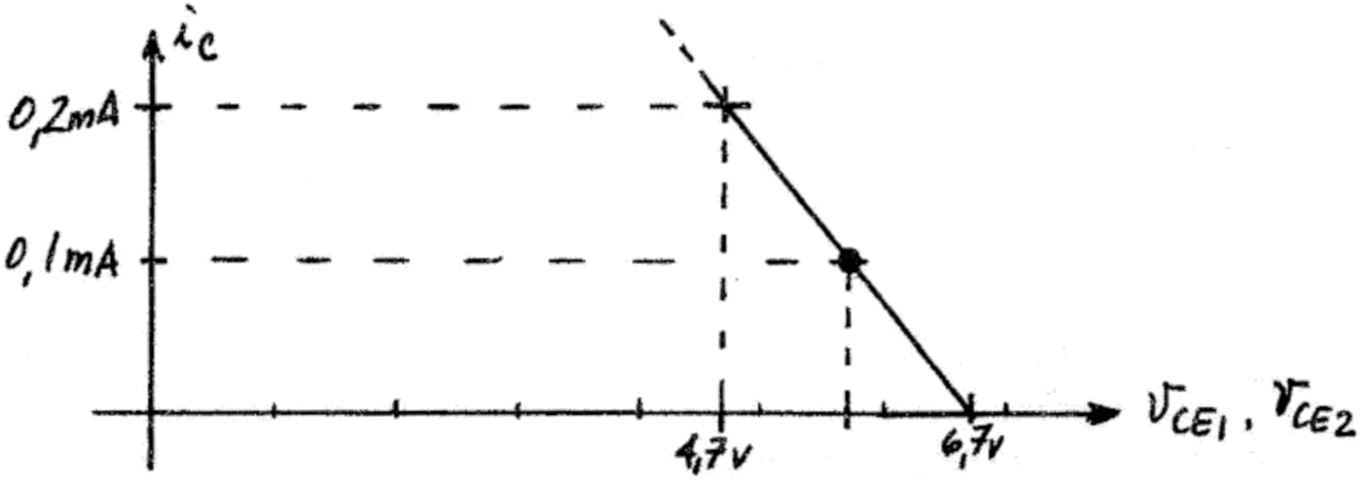
\includegraphics[width=0.8\linewidth]{_fig/multietapas_ejemplo4_recta-de-carga.png}
	\caption{Recta de Carga de \( Q_S \) en Figura \ref{fig:multietapas_ejemplo4-sch}}
	\label{fig:multietapas_ejemplo4_recta-de-carga}
\end{figure}

Otra configuración fuente de corriente, que se utiliza sobre todo en los circuitos integrados, es la denominada "espejo de corriente" que se muestra en la Figura \ref{fig:multietapas_ejemplo4_espejo-de-corriente}. Se hace notar que la base y el emisor de \( Q_1 \) y \( Q_2 \) están unidos; por lo tanto, si los transistores son idénticos, necesariamente la corriente de colector de un transistor es igual a la del otro transistor. 

\begin{figure}[h]
	\centering
	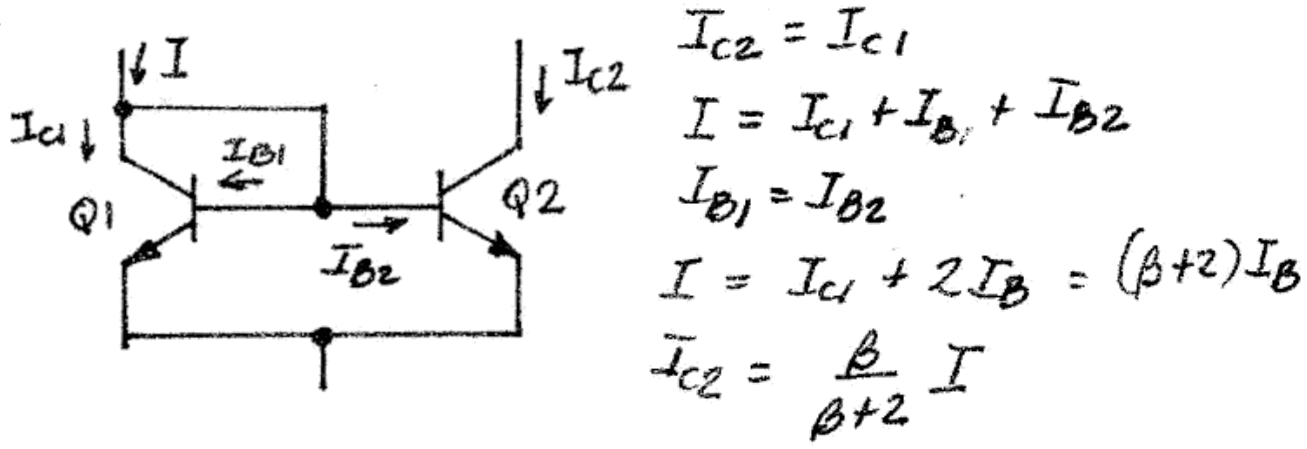
\includegraphics[width=0.8\linewidth]{_fig/multietapas_ejemplo4_espejo-de-corriente.png}
	\caption{Espejo de Corriente}
	\label{fig:multietapas_ejemplo4_espejo-de-corriente}
\end{figure}

\subsection{La característica de transferencia de la configuración diferencial} %p94

La característica de transferencia del amplificador diferencial permite determinar los límites de operación lineal para señales diferenciales. En la Figura \ref{fig:multietapas_par-diferencial-transistores}, se indican las señales de interés del conjunto, de donde se obtienen las siguientes relaciones:

\( -V_{BI} + V_{BE1} - V_{BE2} + V_{B2} = 0 \), de donde

\begin{equation}
	V_{BI} - V_{B2} = V_{BE1} - V_{BE2}
\end{equation}

e

\begin{equation}
	I_{C1} + I_{C2} = I_0 \quad \text{(una constante)}
\end{equation}

Bajo condiciones de equilibrio, \( V_{BI} = V_{B2} \), \( V_{BE1} = V_{BE2} \) e \( I_{C1} = I_{C2} = I_0 /2 \).

Cuando \( V_{BE1} < V_{\gamma} \) (voltaje umbral), \( Q_1 \) estará en la región de corte, \( I_{C1} = 0 \), y toda la corriente pasa por \( Q_2 \), \( I_{C2} = I_0 \). A medida que aumenta \( V_{BE1} \), aumenta \( I_{C1} \) y disminuye \( I_{C2} \). El rango de tensión para el cual la salida puede seguir la entrada viene dado.

\begin{figure}[h]
	\centering
	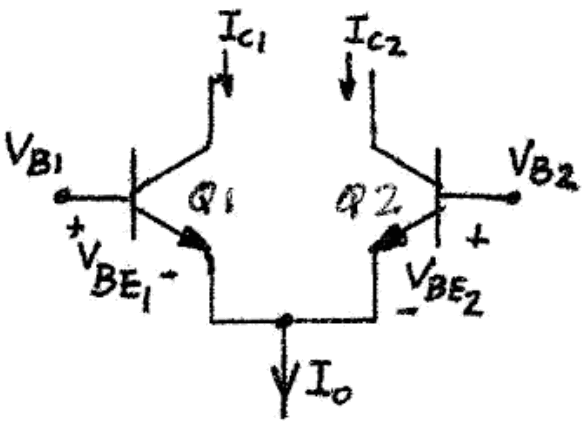
\includegraphics[width=0.5\linewidth]{_fig/multietapas_par-diferencial-transistores.png}
	\caption{La configuración diferencial}
	\label{fig:multietapas_par-diferencial-transistores}
\end{figure}

Por \( \Delta V = R_C I_{\text{TOTAL}} = R_C I_0 \)

La relación exacta entre las tensiones de entrada y las corrientes que circulan por los transistores se encuentra por medio de la ecuación de corriente de una junta \( pn \):

\begin{equation}
	I_E \approx I_S e^{V_{BE}/V_T} \tag{2.37}
\end{equation}

Se tiene

\[
I_0 = I_{E1} + I_{E2} = I_S e^{V_{BE1}/V_T} + e^{V_{BE2}/V_T} = I_S e^{(V_{BI} - V_{B2})/V_T}
\]

de donde

\begin{equation}
	I_{E2} = \frac{I_0}{(1 + e^{(V_{BI} - V_{B2})/V_T})} \tag{2.38}
\end{equation}

y por simetría,

\begin{equation}
	I_{E1} = \frac{I_0}{(1 + e^{-(V_{BI} - V_{B2})/V_T})} \tag{2.39}
\end{equation}

Estas relaciones se grafican en la Figura \ref{fig:multietapas_caracteristicas-par-diferencial}.

Se observa que:
\begin{enumerate}
	\item Cuando \( |V_{BI} - V_{B2}| > 4V_T \), \( \Delta V_T = 104 \) mV a la temperatura ambiental, el circuito ha llegado a un valor extremo, y habrá un transistor en la región de corte.
	\item La pendiente es \( I_0 / 4V_T \), la 1/4 de la de un transistor, y solo para \( |V_{BI} - V_{B2}| < 2V_T = 59 \) mV.
	\item La ganancia es proporcional a la corriente de reposo, ya que es proporcional a \( g_m R_C \); si se quiere cambiar la ganancia, esto se puede lograr modificando la corriente del punto de operación.
\end{enumerate}

\begin{figure}[h]
	\centering
	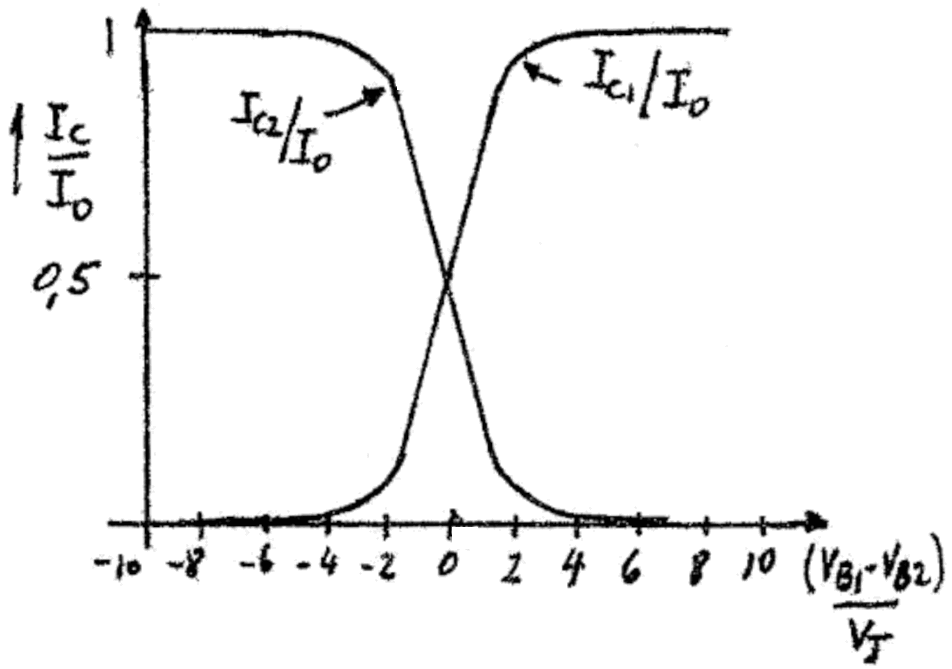
\includegraphics[width=0.8\linewidth]{_fig/multietapas_caracteristicas-par-diferencial.png}
	\caption{La configuración diferencial}
	\label{fig:multietapas_caracteristicas-par-diferencial}
\end{figure}

Hay aplicaciones donde explícitamente la entrada es sencilla pero implícitamente es diferencial, como en el siguiente ejemplo.

\subsubsection{Ejemplo 5}
Dado \( v_s(t) = 1 \sin wt \), hallar y dibujar \( v_o(t) \) del circuito de la Figura \ref{fig:multietapas_ejemplo5-sch}.

\begin{figure}[h]
	\centering
	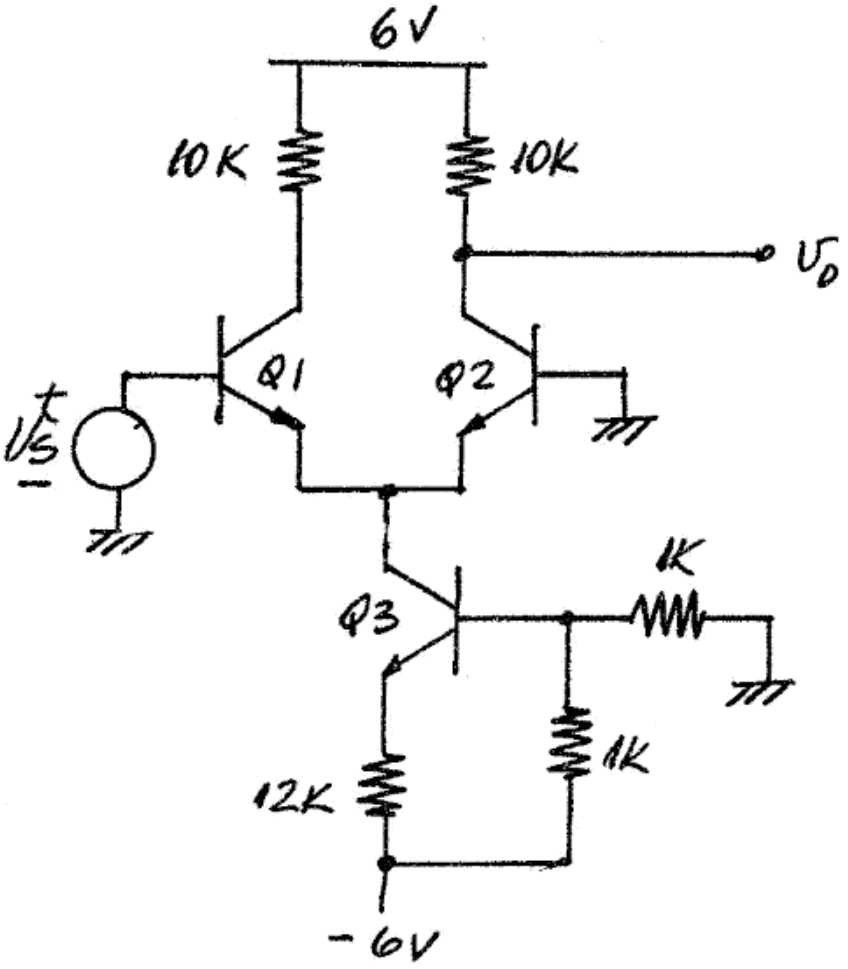
\includegraphics[width=0.4\linewidth]{_fig/multietapas_ejemplo5-sch.png}
	\caption{Circuito de Ejemplo}
	\label{fig:multietapas_ejemplo5-sch}
\end{figure}

\textbf{Solución:} A pesar de que solo aparece una entrada, podemos reconocer la configuración diferencial y analizarla como tal. Haciendo: \( V_1 = v_s \), \( V_2 = 0 \), de donde \( V_d = V_1 - V_2 = V_s \), y \( V_c = \frac{(V_1 + V_2)}{2} = \frac{V_s}{2} \).

Entonces el circuito es el mismo de la Figura \ref{fig:multietapas_ejemplo4_comp-termica}; la fuente de corriente suministra \( 0.2 \text{mA} \), que en condiciones de reposo se reparte equitativamente entre los 2 transistores, de modo que \( V_o (\text{DC}) = 6V - 10K(0.1mA) = 5V \). La fuente de corriente \( Q_3 \) hace que la ganancia de modo común sea prácticamente igual a 0. Entonces, si \( A_c \approx 0 \) y \( v_d = v_s \), nos queda \( v_o = A_d v_s \), donde \( A_d \) necesariamente es positiva.

Si se aplica el Teorema de Bisección, nos queda el siguiente circuito, la Figura \ref{fig:multietapas_ejemplo5-biseccion}.

\begin{figure}[h]
	\centering
	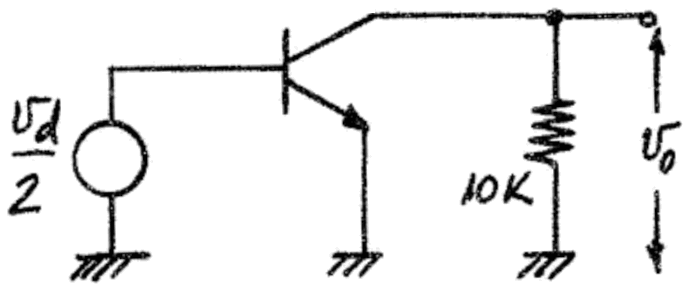
\includegraphics[width=0.6\linewidth]{_fig/multietapas_ejemplo5-biseccion.png}
	\caption{Aplicando Teorema de Bisección}
	\label{fig:multietapas_ejemplo5-biseccion}
\end{figure}

De aquí:

\[
\frac{v_o}{(v_d /2)} = -\beta \cdot 10K / V_T = - g_m 10k = - 0.1mA \cdot 10K / 25mV
\]

o 

\[
A_d = \frac{v_o}{v_d} = -1K / 50 = -20.
\]

En la zona lineal, la ganancia \( v_o / v_s = 20 \). La zona lineal es de una extensión limitada, ya que de su valor de \( 5V \) en DC, \( v_o \) solo puede variar hasta \( 6V \) en una dirección (\( i_{C2} = 0 \)), y hasta \( 4V \) en la otra (\( i_{C2} = 0.2mA, i_{C1} = 0 \)). Es decir, la máxima variación de \( v_o \) es \( 1V \) en cada dirección.

Para causar esta variación, \( v_s \) variará \( 1V / 20 = 50mV \). Mientras \( v_s > 50mV \), entonces \( v_o = 6V \), y cuando \( v_s < -50mV \), \( v_o = 4V \). Habrá solo un trayecto corto de \( v_s \) en que se amplifica linealmente. El resultado se muestra en la Figura \ref{fig:multietapas_ejemplo5-respuesta}.

\begin{figure}[h]
	\centering
	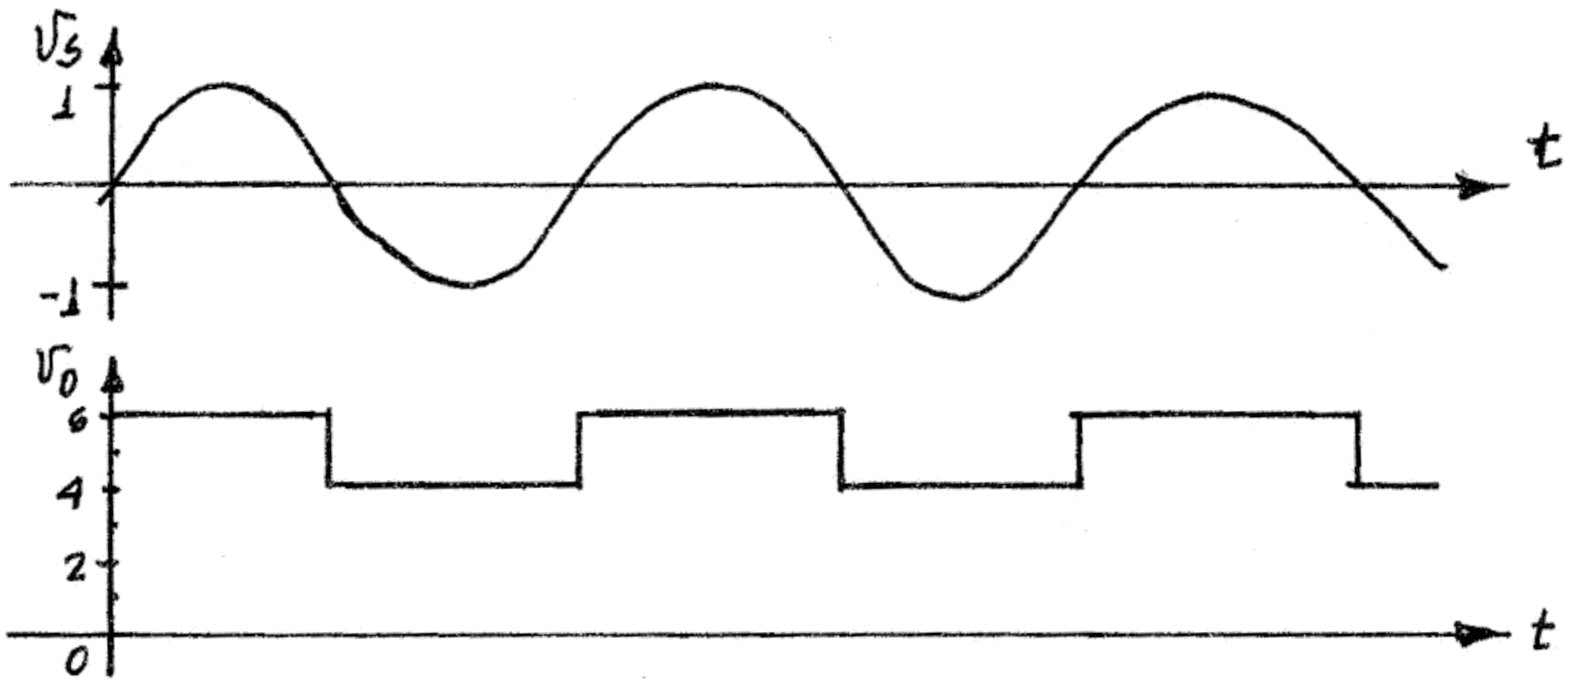
\includegraphics[width=0.8\linewidth]{_fig/multietapas_ejemplo5-respuesta.png}
	\caption{Respuesta \( V_s \) y \( V_o \)}
	\label{fig:multietapas_ejemplo5-respuesta}
\end{figure}

En resumen, la configuración diferencial anterior es una solución excelente a los requerimientos de un amplificador de corriente contínua, con buena ganancia y buena estabilidad térmica. Esta configuración simétrica con salida sencilla a su vez ha dado lugar a modificaciones por diversos motivos. A continuación la analizaremos cuando la salida es diferencial y cuando el circuito no es simétrico.

\subsection{Configuración entrada diferencial, salida diferencial} %p98

En la Figura \ref{fig:multietapas_amp-diferencial_salida-diferencial} se representa un esquema de este tipo de circuito

\begin{figure}[h]
	\centering
	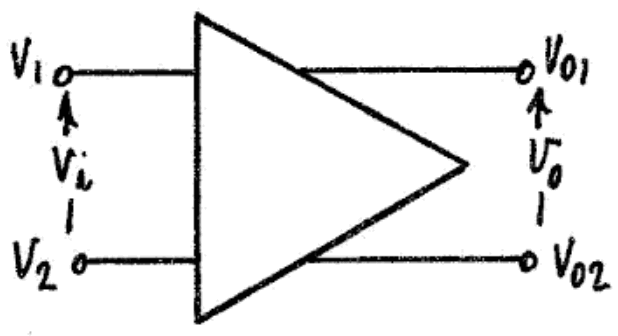
\includegraphics[width=0.4\linewidth]{_fig/multietapas_amp-diferencial_salida-diferencial.png}
	\caption{Amplificador Diferencial con Salida Diferencial}
	\label{fig:multietapas_amp-diferencial_salida-diferencial}
\end{figure}

Tenemos:

\[ 
V_o = V_{o1} - V_{o2}
\]

\[ 
V_{o1} = A_{11} V_1 + A_{21} V_2
\]

\[
V_{o2} = A_{12} V_1 + A_{22} V_2
\]

de donde

\[
V_o = (A_{11} - A_{12}) V_1 + (A_{21} - A_{22}) V_2
\]

Para circuitos simétricos se cumple que:

\begin{equation} \label{equ:multietapas_amp-diferencial_salida-diferencial_relacion}
	A_{22} = A_{11} \quad \text{y} \quad A_{21} = A_{12}
\end{equation}

de donde \( A_{11} - A_{12}) = -(A_{21} - A_{22}) \)
y \( V_o = (A_{11} - A_{22})(V_1 - V_2) = A_d V_d \)

es decir, la ganancia de modo común es idénticamente igual a \( 0 \).

La salida diferencial elimina cualquier componente común.

Si hay diferencias de los componentes, entonces las relaciones de la ecuación \ref{equ:multietapas_amp-diferencial_salida-diferencial_relacion} no son correctas. Por ejemplo, si:

\begin{equation}
	A_{22} = A_{11} + \Delta_1 \quad \text{y} \quad A_{21} = A_{12} + \Delta_2
\end{equation}

entonces,

\[
V_o = (A_{11} - A_{12})V_1 - (A_{11} - A_{12})V_2 + (\Delta_2 - \Delta_1)
\]	
\[
V_o = (A_{11} - A_{12})(V_1 - V_2) + (\Delta_2 - \Delta_1)V_2
\]

de donde evidentemente habrá una ganancia de modo común.

\subsection{Circuito diferencial no simétrico} %p99

Existen configuraciones diferenciales que no son perfectamente simétricas como en los circuitos anteriores. Para tales circuitos el Teorema de Bisección no es aplicable sencillamente por que no se cumplen las condiciones necesarias para su aplicación. Tendremos la obligación de analizar el circuito de otra forma. A continuación veremos varios casos utilizando 1) Circuito diferencial con la salida no balanceada, 2) Circuito diferencial con la fuente no balanceada.

\subsection{Circuito diferencial no Balanceado - Uso de Modelo de Pequeña Señal} %p99

En la Figura \ref{fig:multietapas_conf-diferencial_modelo} tenemos un configuración diferencial, en donde los circuitos de base son simétricos, y la polarización de los emisores con fuentes de corriente es simétrica. Sin embargo, los circuitos de colector son distintos. Se puede analizar este circuito si se resuelve como un todo, reemplazando los transistores por su modelo equivalente y trabajando con el conjunto resultante de nodos y mallas. Para este circuito, nos queda el equivalente de la Figura \ref{fig:multietapas_conf-diferencial_equivalente}.

\begin{figure}[h]
	\centering
	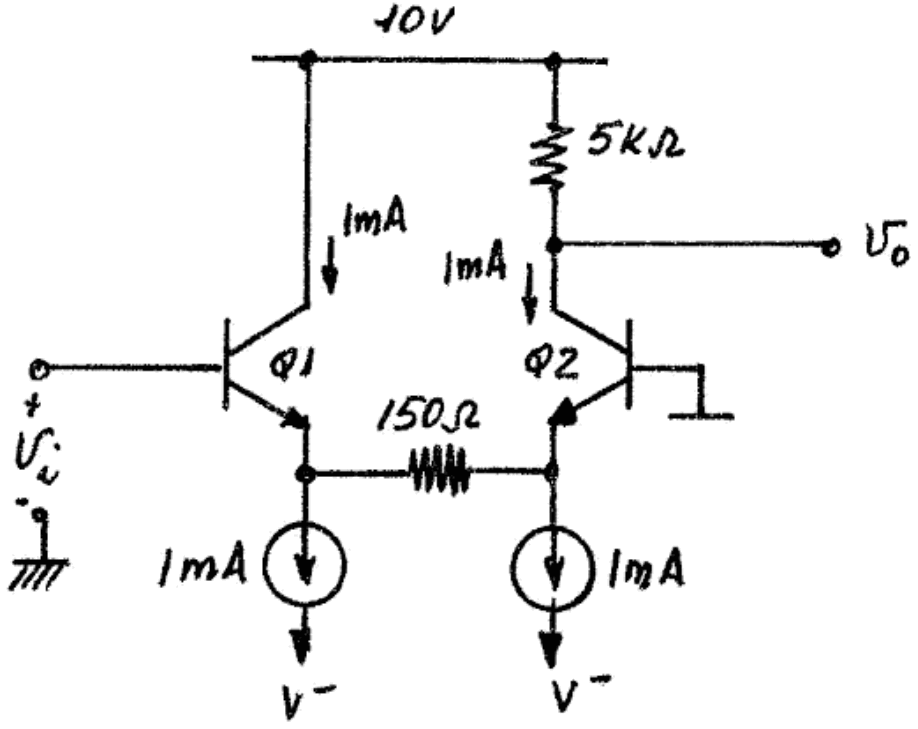
\includegraphics[width=0.6\linewidth]{_fig/multietapas_conf-diferencial_modelo.png}
	\caption{Configuración diferencial, circuito}
	\label{fig:multietapas_conf-diferencial_modelo}
\end{figure}

\begin{figure}[h]
	\centering
	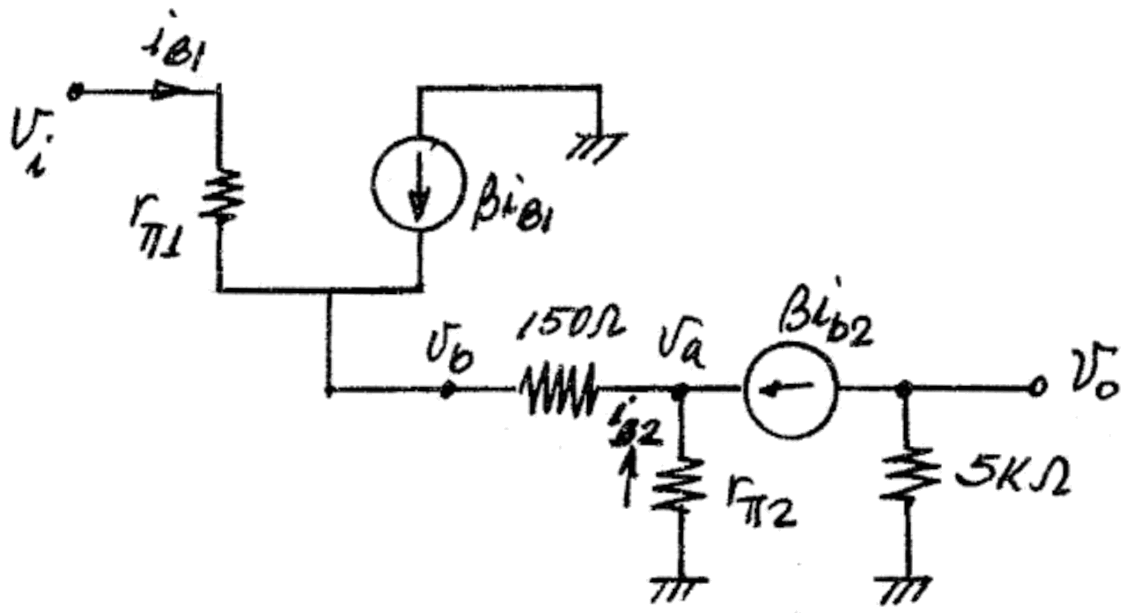
\includegraphics[width=0.6\linewidth]{_fig/multietapas_conf-diferencial_equivalente.png}
	\caption{Configuración diferencial, equivalente}
	\label{fig:multietapas_conf-diferencial_equivalente}
\end{figure}

De ésta figura se obtiene
\[
V_o/V_a = 85k/r_{\pi 2}
\]
\[
V_a/V_b = (r_{\pi 2}/(\beta+1))/(150 + r_{\pi 2}/(\beta+1))
\]
\[
V_b/V_i = (\beta+1)(150 + r_{\pi 2}/(\beta+1)) / (r_{\pi 1} + (\beta+1)(150 + r_{\pi 2}/(\beta+1)))
\]
\[
V_o/V_i = 85K/(r_{\pi 1} + (\beta+1)(150 + r_{\pi 2}/(\beta+1)))
\]

con \( r_{\pi 2} = 100 \cdot 25 \text{mV}/1 \text{mA} = 2500 \Omega \)

da \( V_o/V_i = 25 \)

y \( R_i = r_{\pi 1} + (\beta+1)(150 + r_{\pi 2}/(\beta+1)) = 20.2K\Omega \)

\subsubsection{Ejercicio 6}

Compare el circuito de la Figura \ref{fig:multietapas_ejemplo6-sch-a} con el de la Figura \ref{fig:multietapas_ejemplo6-sch-b}. Sin necesidad de hacer cálculos, ¿cuál de los dos circuitos presenta mayor ancho de banda? ¿Por qué?, ¿El circuito con peor ancho de banda tendrá alguna característica mejor para compensar su defecto?

\begin{figure}[h]
	\centering
	\subfloat[A]
	{
		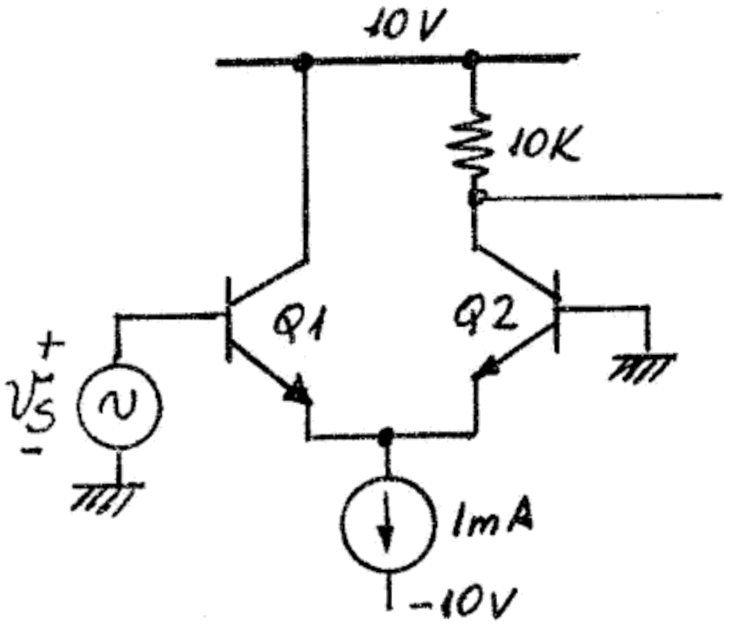
\includegraphics[width=0.46\linewidth]{_fig/multietapas_ejemplo5-sch-a.png}
		\label{fig:multietapas_ejemplo6-sch-a}
	}
	\subfloat[B]
	{
		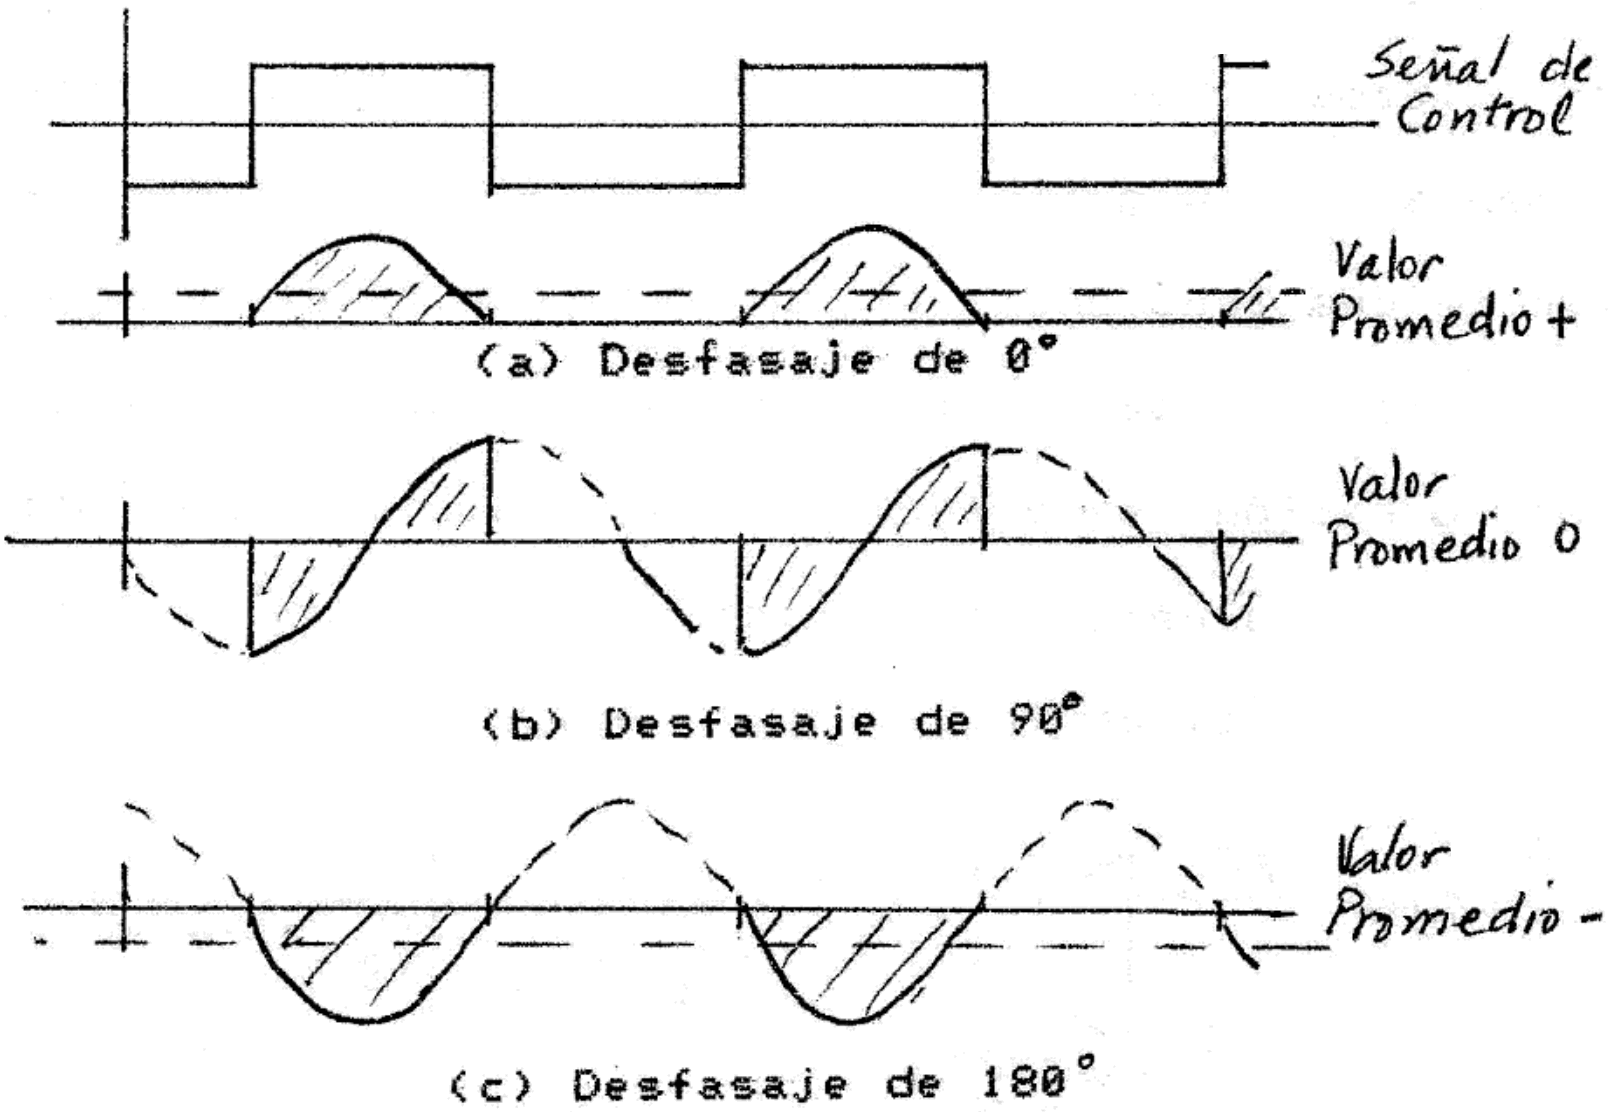
\includegraphics[width=0.46\linewidth]{_fig/multietapas_ejemplo5-sch-b.png}
		\label{fig:multietapas_ejemplo6-sch-b}
	}
	\caption{Circuito de ejemplo}
	\label{fig:multietapas_ejemplo6-sch}
\end{figure}


\subsection{Circuito diferencial no Balanceados las Fuentes de Entrada} %p101

En la Figura \ref{fig:multietapas_conf-diferencial_no-bal} se observa que el circuito de base de Q1 tiene una resistencia de 10k que no aparece en la base de Q2. Por lo tanto están desbalanceados los circuitos de polarización y

\begin{figure}[h]
	\centering
	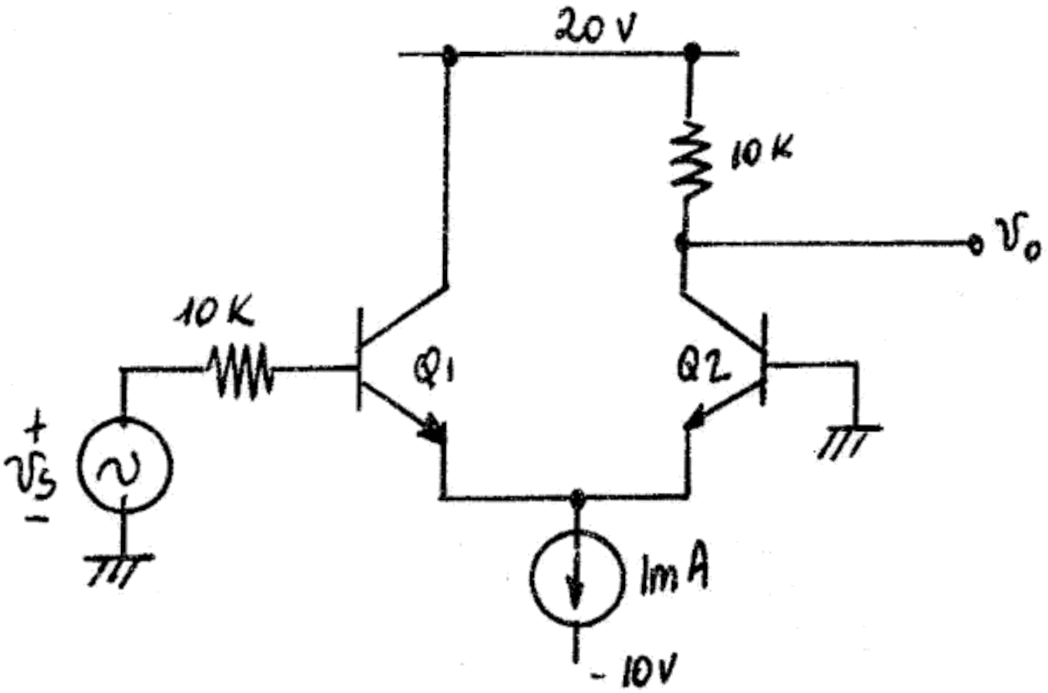
\includegraphics[width=0.4\linewidth]{_fig/multietapas_conf-diferencial_no-bal.png}
	\caption{Configuración diferencial, equivalente}
	\label{fig:multietapas_conf-diferencial_no-bal}
\end{figure}

la corriente de polarización de la fuente de corriente no va circular en partes iguales por ambos transistores. Para hallar el punto de operación, tenemos la ecuación de malla

\begin{equation} \label{equ:conf-diferencial_no-bal_malla}
	(i_{E1}/(\beta+1))10k + v_{BE1} = v_{BE2}
\end{equation}

y la ecuación de nodo

\begin{equation} \label{equ:conf-diferencial_no-bal_nodo}
	i_{E1} + i_{E2} = 1 \text{mA}
\end{equation}

con la salvedad que en lugar de tomar $v_{BE}$ fijo, es necesario considerar la pequeña diferencia que surge al circular diferentes cantidades de corriente de acuerdo a la relación

\[
v_{BE} = v_T \ln(i_E/I_S)
\]

En este caso no hace falta conocer $I_S$ ya que se requiere solamente la diferencia entre $v_{BE1}$ y $v_{BE2}$ de donde desaparece el parámetro $I_S$, como en la siguiente ecuación

\[
v_{BE1} - v_{BE2} = v_T \ln(i_{E1}/i_{E2})
\]

y la ecuación \ref{equ:conf-diferencial_no-bal_malla} se convierte en

\[
(i_{E1}/(\beta+1))10k + v_T \ln(i_{E1}/i_{E2}) = 0
\]

e incorporando la ecuación \ref{equ:conf-diferencial_no-bal_nodo} queda

\[
(i_{E1}/(\beta+1))10k + v_T \ln(i_{E1}/(1\text{mA} - i_{E1})) = 0
\]

Esta es una ecuación no-lineal, cuya solución se encuentra iterativamente, tal como se indica en la siguiente tabla:

\begin{center}
	\begin{tabular}{ccc}
		\hline
		1 & 2 & 3 \\
		\hline
		$i_{E1}$ & $(i_{E1}/(\beta+1))10k$ & $V_T \ln(i_{E1}/(1\text{mA} - i_{E1}))$ \\
		\hline
		0.49 & 0.0485 & -0.00104 \\
		0.45 & 0.0445 & -0.0052 \\
		0.4 & 0.0396 & -0.0105 \\
		0.35 & 0.0346 & -0.016 \\
		0.3 & 0.0297 & -0.022 \\
		0.26 & 0.02574 & -0.0271 \\
		0.27 & 0.02673 & -0.02586 \\
		\hline
	\end{tabular}
\end{center}

En esta tabla se procura hacer el valor de la columna 2 igual al valor negativo de la columna 3. Con el valor inicial de $i_{E1}$ el valor absoluto de la columna 2 es muy superior al valor absoluto de la columna 3. A medida que disminuye $i_{E1}$, disminuye el valor absoluto de la columna 2 y aumenta el valor absoluto de el valor absoluto de la columna 2 y aumenta el valor absoluto de la columna 3. En la penúltima fila, la columna 3 supera en valor a la columna 2; de aquí en adelante se va ajustando el valor de $i_{E1}$ en la dirección apropiada hasta lograr una cierta precisión en la diferencia entre la columna 2 y 3. Se hace notar la relación entre $i_{E1}$ e $i_{E2}$ que en vez de estar equilibradas las corrientes, tenemos \( i_{E1} = 0.27 \text{mA} \) e \( i_{E2} = 0.73 \text{mA}\).

\subsubsection{Ejemplo 7}
Para el circuito de la Figura \ref{fig:multietapas_ejemplo7-sch}:

\begin{enumerate}
	\item[a)] Hallar \( I \)
	\item[b)] Hallar la corriente de polarización de entrada
	\item[c)] Hallar el Rango de Modo Común de Entrada
	\item[d)] Hallar la Resistencia de Entrada Diferencial
	\item[e)] Hallar la Ganancia Diferencial
	\item[f)] Hallar la Ganancia de Modo Común si las \( RC \) son parejas en un \( 1\% \) y si \( R_o \) de \( Q3 \) es \( 5.9 M\Omega \)
	\item[g)] Hallar la Relación de Rechazo de Modo Común
\end{enumerate}

\begin{figure}[h]
	\centering
	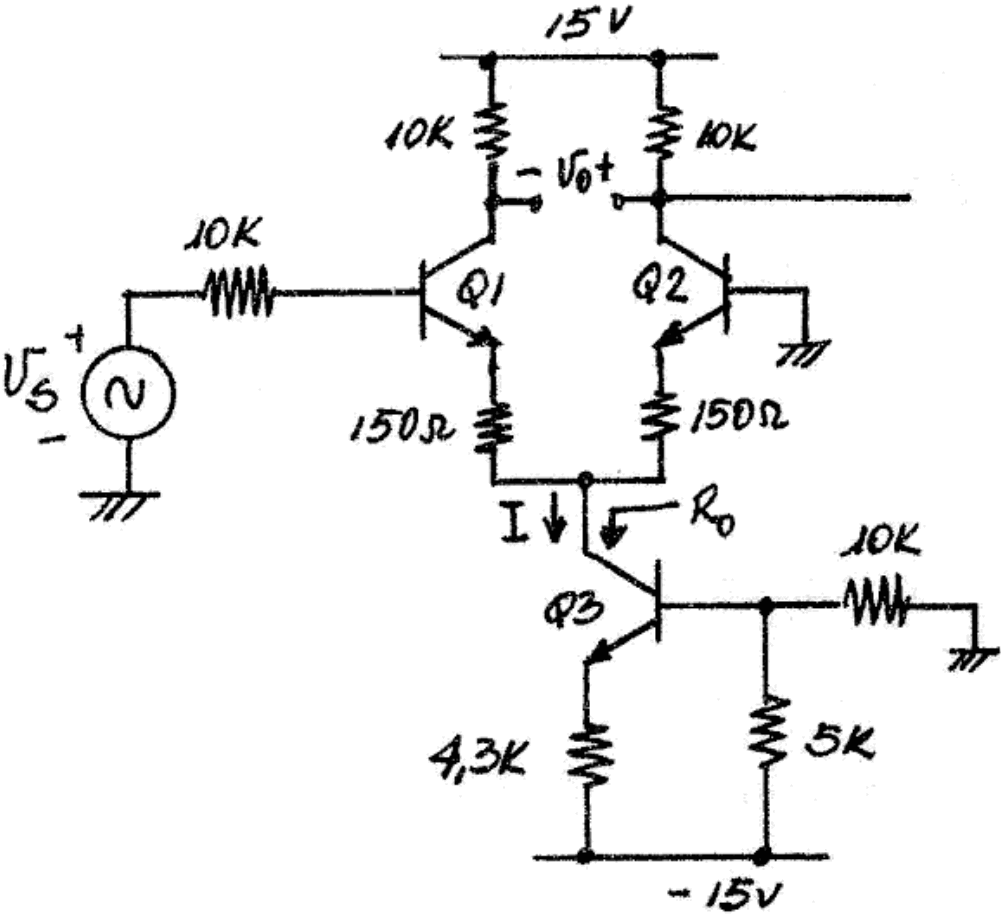
\includegraphics[width=0.6\linewidth]{_fig/multietapas_ejemplo7-sch.png}
	\caption{Circuito de Ejemplo}
	\label{fig:multietapas_ejemplo7-sch}
\end{figure}

\textbf{Solución:}

\textbf{a)} Para hallar I se crea un circuito equivalente de Thevenin en la base de Q3, quedando $R_{Th} = 10k // 5k = 3,33k$, $V_{Th} = -10V$, de donde $I_{E3} = (15 - 10 - 0,7)/(4,3k + 3,3k/101) \approx 1$ mA

\textbf{b)} Si I se divide en partes iguales, implica cada transistor se polariza con 0,5 mA de donde $i_B = 5 \mu A$. Sin embargo en este caso se observa que los circuitos de base no son simétricos por lo que requiere precisar iterativamente la distribución de I. Tenemos el siguiente par de ecuaciones:

\[
(i_{E1}/101)10k + v_{BE1} + i_{E1}150 = v_{BE2} + i_{E2}150
\]
\[
i_{E1} + i_{E2} = 1 \text{mA}
\]

y su resolución da \( i_{E1} = 0.4 \text{mA}\) e \( i_{E2} = 0.6 \text{mA} \), con lo que \( v_{BE1} = 0.695 V \) y \( v_{BE2} = 0,705 V \).

\textbf{c)} El límite inferior del rango de modo común lo determina la región activa de \( Q3 \). Si se toma saturación como \( v_{CE} = 0.2 V \), entonces \( Q3 \) entra en saturación cuando \( V_{B3} = -10.7 + 0.2 = -10.5 V \) que conlleva a \( V_{B1} = V_{B2} = -10.5 + 0.7 = -9.8 V \).

El límite superior se establece con mantener \( Q1 \) y \( Q2 \) en la región activa aún bajo la condición de la máxima excursión de la señal de salida, \( \Delta V = \Delta i_C R_C = 1 \text{mA}(10k) = 10 V \). Entonces la tensión mínima en el colector de uno de estos transistores es \( 15 - 10 = 5V \), y el nivel común de entrada máximo será \( 5 - 0.2 + 0.7 = 5.5 V \).

El rango de modo común es \( -9.3V, 5.5V) \).

\textbf{d)} La resistencia de entrada diferencial se destaca del siguiente diagrama, de donde , ver Figura \ref{fig:multietapas_ejemplo7-sch-rid}.

\begin{figure}[h]
	\centering
	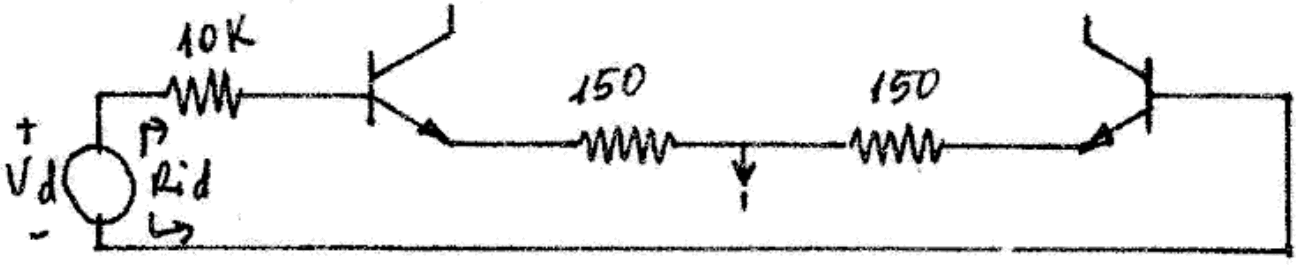
\includegraphics[width=0.6\linewidth]{_fig/multietapas_ejemplo7-sch-rid.png}
	\caption{Circuito de Ejemplo}
	\label{fig:multietapas_ejemplo7-sch-rid}
\end{figure}

\textbf{e)} La ganancia de modo diferencial la encontraremos de dos modos: por medio del modelo de pequeña señal, y utilizando el Teorema de Bisección.

En la Figura \ref{fig:multietapas_ejemplo7-pequena-senal}, se plantea el modelo de pequeña señal del circuito anterior. De aquí se obtiene:

\[
\frac{V_o^+}{V_s} = (\frac{V_o^+}{V_a})(\frac{V_a}{V_b})(\frac{V_b}{V_s})
\]
\[
\frac{V_o^+}{V_s} = 192.3 \times 0.1465 \times 0.7 = 19.7
\]

\[
\frac{V_o^-}{V_s} = \frac{-810k}{(10k + r_{\pi 1} + (\beta+1)(300 + r_{\pi 2}/(\beta+1)))} = -19.72
\]
\[
\frac{V_o}{V_s} = \frac{V_o^+ - V_o^-}{V_s} = 19.72 - (-19.72) = 39.94
\]

\begin{figure}[h]
	\centering
	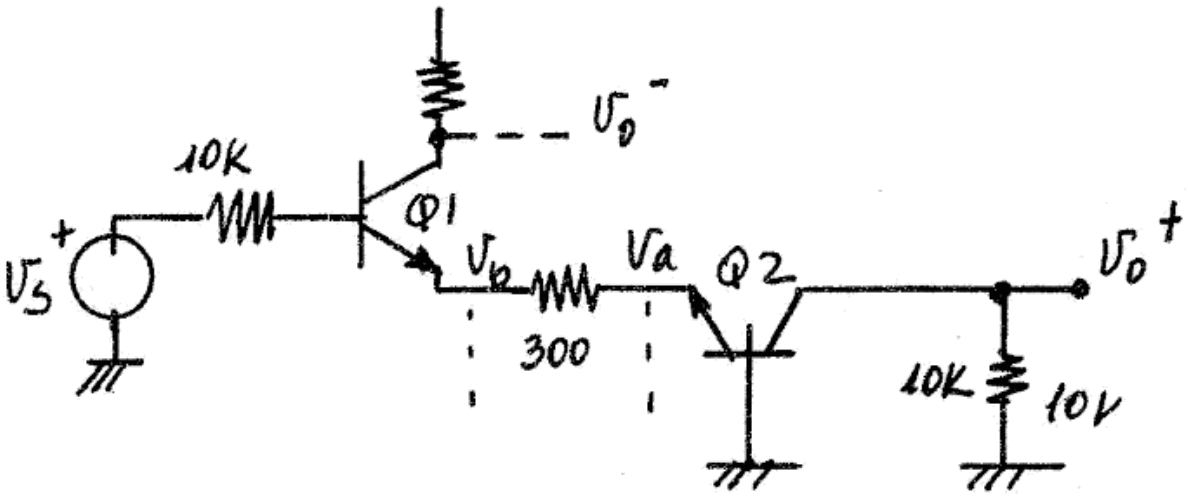
\includegraphics[width=0.4\linewidth]{_fig/multietapas_ejemplo7-pequena-senal.png}
	\caption{Circuito de Ejemplo, aplicando modelo de pequeña señal}
	\label{fig:multietapas_ejemplo7-pequena-senal}
\end{figure}

Con el Teorema de Bisección, trabajamos con el circuito como si no existiera la resistencia de \( 10K\Omega \), tal como se indica en la Figura \ref{fig:multietapas_ejemplo7-biseccion-a}, con el cual se obtiene \( V_o/V_d = 49.5 \). Posteriormente se aplica la fuente con su resistencia de \( 10K\Omega \) en serie, para quedarnos con una cascada de redes, como en la Figura \ref{fig:multietapas_ejemplo7-biseccion-b}, cuya ganancia global es

\begin{figure}[h]
	\centering
	\subfloat[A]
	{
		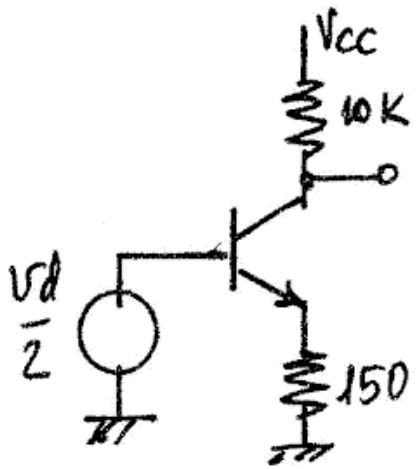
\includegraphics[width=0.46\linewidth]{_fig/multietapas_ejemplo7-biseccion-a.png}
		\label{fig:multietapas_ejemplo7-biseccion-a}
	}
	\subfloat[B]
	{
		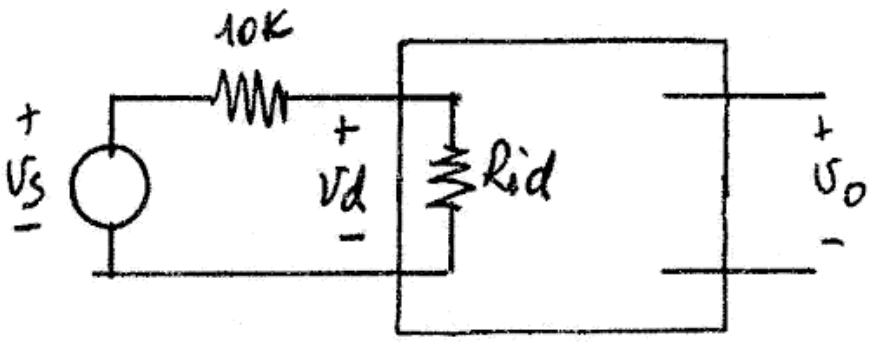
\includegraphics[width=0.46\linewidth]{_fig/multietapas_ejemplo7-biseccion-b.png}
		\label{fig:multietapas_ejemplo7-biseccion-b}
	}
	\caption{Circuito de ejemplo}
	\label{fig:multietapas_ejemplo7-biseccion}
\end{figure}

\[
v_o/v_s = (v_o/v_d)(v_d/v_s) = 49,5(40,4k)/(50,4k) = 39,76
\]

es decir, prácticamente el mismo resultado anterior.

\textbf{f)} En teoría esta configuración no tiene una ganancia de modo común excepto por diferencias en el emparejamiento de los componentes. Con $R_e$ disparejos, y considerando a $R_o$ de Q3 = 5,9 M$\Omega$, la ganancia de modo común viene dada por

\[
A_{cm} = (R_e/2R_o)(\Delta R_C/R_C) 
\]
\[
A_{cm} = 10k(0,01)/2 \times 5,9 \times 10^6 = 8,47 \times 10^{-6}
\]

\textbf{g)} La Relación de Rechazo de Modo Común viene dada por:

\[
\text{CMRR} = 20 \log |39,44/8,47 \times 10^{-6}| = 133 \text{ dB}
\]

\subsection{Par Diferencia con FET} %p106

En la Figura \ref{fig:multietapas_conf-diff-fet} se muestra una configuración diferencial con FET.

\begin{figure}[h]
	\centering
	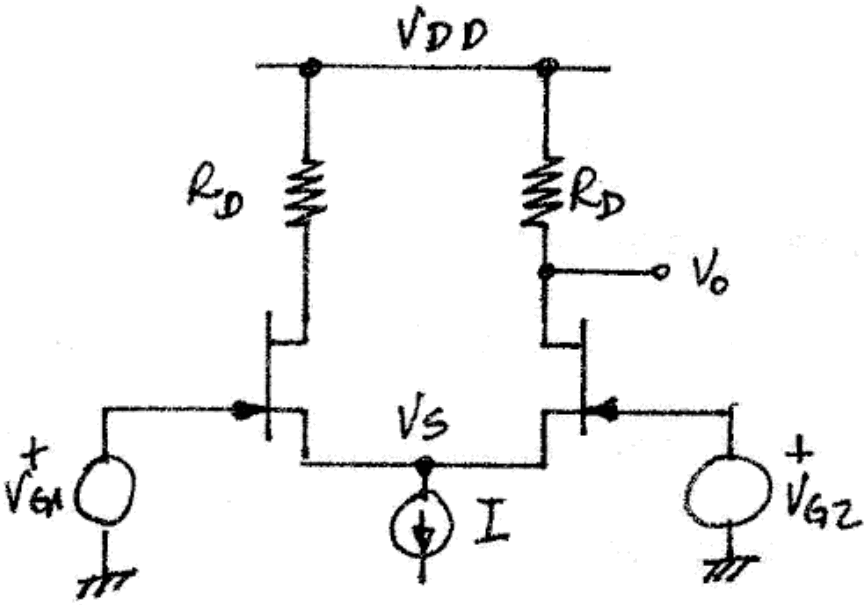
\includegraphics[width=0.4\linewidth]{_fig/multietapas_conf-diff-fet.png}
	\caption{Circuito configuracion diferencial con FET}
	\label{fig:multietapas_conf-diff-fet}
\end{figure}

Si se supone los transistores en la región de saturación entonces:

\begin{equation}
	i_{D1} = i_{DSS}(1 - \frac{v_{GS1}}{V_p})^2 = i_{DSS}(1 - \frac{v_{G1} - v_s}{V_p})^2
\end{equation}
\begin{equation}
	i_{D2} = i_{DSS}(1 - \frac{v_{GS2}}{V_p})^2 = i_{DSS}(1 - \frac{v_{G2} - v_s}{V_p})^2
\end{equation}
\begin{equation}
	\sqrt{i_{D1}} = \sqrt{i_{DSS}}(1 - \frac{v_{GS1}}{V_p})
\end{equation}
\begin{equation}
	\sqrt{i_{D1}} - \sqrt{i_{D2}} = \sqrt{i_{DSS}}(\frac{v_{GS2} - v_{GS1}}{-V_p}) = \sqrt{i_{DSS}}(\frac{v_{id}}{-V_p})
\end{equation}

pero $i_{D1} + i_{D2} = I$. Entonces de la ecuación anterior

\begin{equation}
	i_{D1} = \frac{I}{2} + v_{id} \sqrt{\frac{2I_{DSS}}{I}} - (\frac{v_{id}}{V_p})^2 (\frac{I_{DSS}}{I})^2
\end{equation}
\begin{equation}
	i_{D2} = \frac{I}{2} - v_{id} \sqrt{\frac{2I_{DSS}}{I}} - (\frac{v_{id}}{V_p})^2 (\frac{I_{DSS}}{I})^2
\end{equation}

para que un transistor se lleve toda la corriente requiere

\begin{equation}
	\frac{I}{-2V_p} \sqrt{\frac{2I_{DSS}}{I}} - (\frac{v_{id}}{V_p})^2 (\frac{I_{DSS}}{I})^2 = \frac{I}{2} 
\end{equation}
o
\begin{equation}
	|V_{id}/V_p| = \sqrt{I/I_{DSS}} \tag{2.47b}
\end{equation}

Para hallar otras características de la configuración, como por ejemplo la ganancia, puede utilizarse el Teorema de Bisección. Para entrada diferencial, salida sencilla se obtiene

\[
V_o/V_d = \frac{g_m R_d}{2}
\]

\subsection{La etapa de salida} %107
El circuito de la Figura \ref{fig:multietapas_cascada-etapa-ec} generalmente se acoplará a la carga a través de un condensador, tal como se muestra en la Figura \ref{fig:multietapas_etapa-salida}.

\begin{figure}[h]
	\centering
	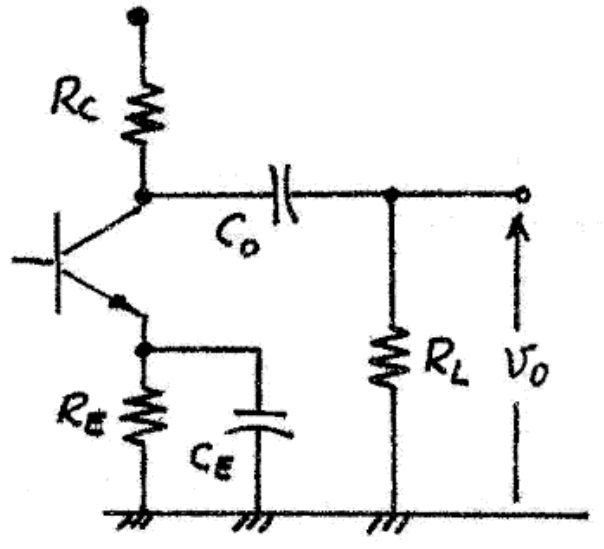
\includegraphics[width=0.4\linewidth]{_fig/multietapas_etapa-salida.png}
	\caption{Circuito de etapa de salida con condensador de acople}
	\label{fig:multietapas_etapa-salida}
\end{figure}

Para el amplificador de continua, queda por obtener una configuración de acoplamiento directo para la etapa de salida.

Una configuración muy buena y popular para la salida que permite acoplamiento directo a la carga es la de simetría complementaria que se muestra en la Figura \ref{fig:multietapas_etapa-salida_simetria-complementaria}. El nivel de continua de la salida es \( 0 \), y la resistencia de salida, \( R_o \), es pequeña. El transistor NPN de arriba conduce para \( V_i \) positivo, y el transistor PNP de abajo conduce para \( V_i \) negativo.

\begin{figure}[h]
	\centering
	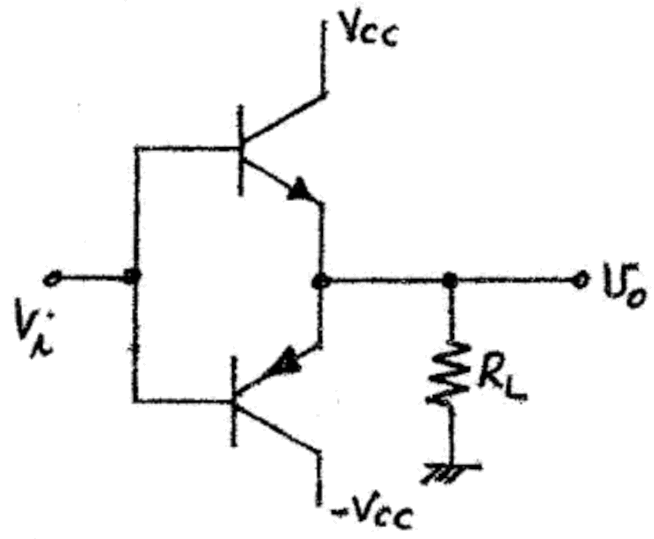
\includegraphics[width=0.4\linewidth]{_fig/multietapas_etapa-salida_simetria-complementaria.png}
	\caption{Circuito de etapa de salida con simetria complementaria}
	\label{fig:multietapas_etapa-salida_simetria-complementaria}
\end{figure}

La configuración tiene el defecto de que \( V_i \) tiene que superar el nivel umbral de tensión en las juntas pn antes de que el transistor correspondiente pueda conducir. La característica de transferencia se muestra en la Figura \ref{fig:multietapas_etapa-salida_característica-transferencia}, donde \( V_\gamma = 0.6 \) para silicio y \( V_\gamma = 0.2 \) para germanio.

\begin{figure}[h]
	\centering
	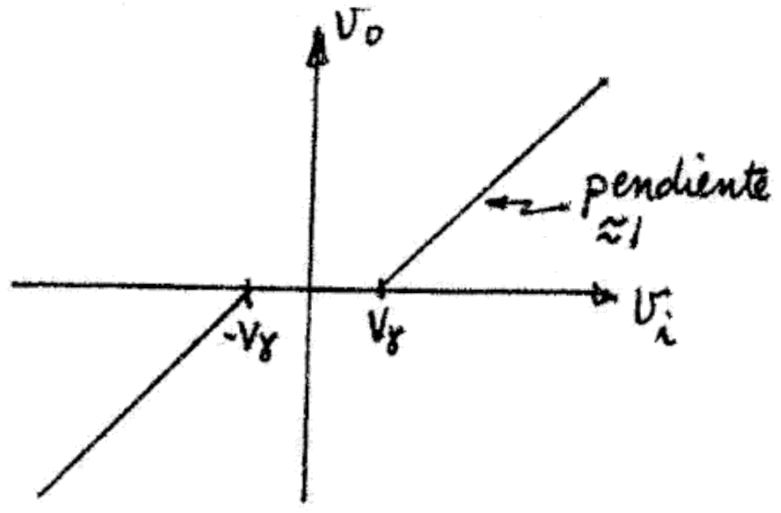
\includegraphics[width=0.4\linewidth]{_fig/multietapas_etapa-salida_característica-transferencia.png}
	\caption{Característica de Transferencia}
	\label{fig:multietapas_etapa-salida_característica-transferencia}
\end{figure}

Esto se puede superar con un esquema de polarizar los transistores al borde de corte, o en la región activa, Figura \ref{fig:multietapas_etapa-salida_polarizacion-diodos} y \ref{fig:multietapas_etapa-salida_polarizacion-resistor}, o utilizar un esquema de retroalimentación para eliminar la distorsión, la Figura \ref{fig:multietapas_etapa-salida_polarizacion-retro}. En los circuitos de la Figura \ref{fig:multietapas_etapa-salida_polarizacion-diodos}, los diodos son polarizados en conducción por las resistencias de base, \( R_B \), de modo que al subir el nivel de entrada sube la señal de base del transistor y varia proporcionalmente la señal de salida.

\begin{figure}[h]
	\centering
	\subfloat[Polarización con diodos]
	{
		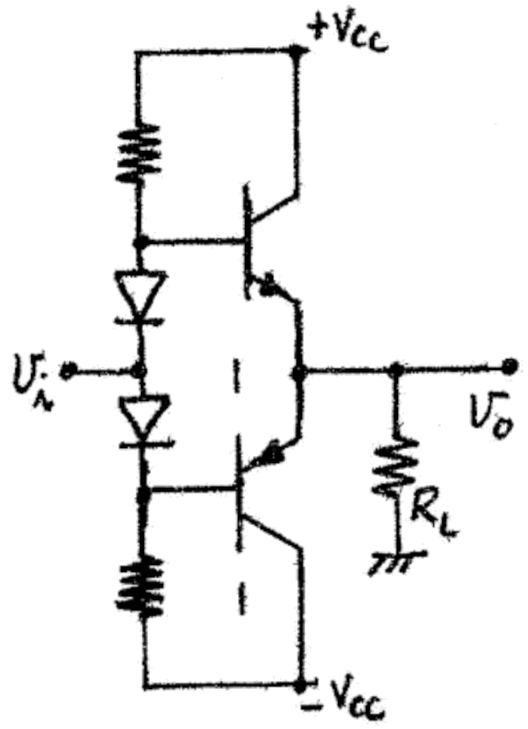
\includegraphics[width=0.28\linewidth]{_fig/multietapas_etapa-salida_polarizacion-diodos.png}
		\label{fig:multietapas_etapa-salida_polarizacion-diodos}
	}
	\subfloat[Con resistencias]
	{
		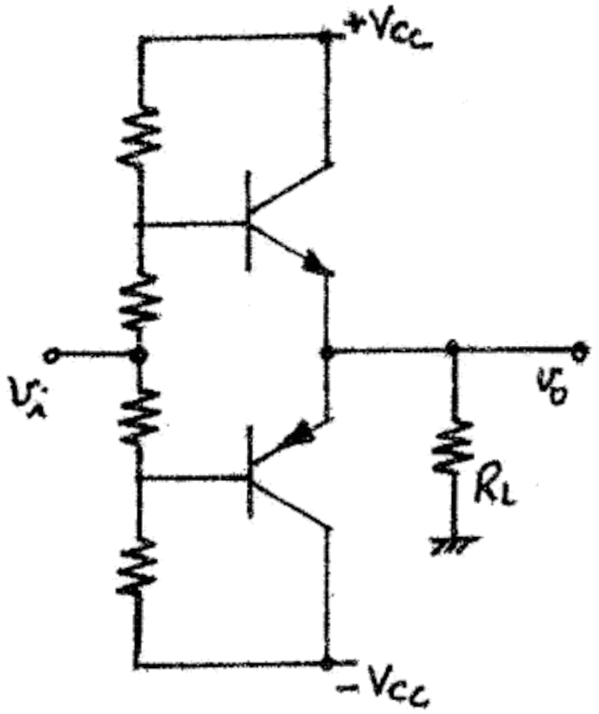
\includegraphics[width=0.28\linewidth]{_fig/multietapas_etapa-salida_polarizacion-resistor.png}
		\label{fig:multietapas_etapa-salida_polarizacion-resistor}
	}
	\subfloat[Uso de retroalimentación]
	{
		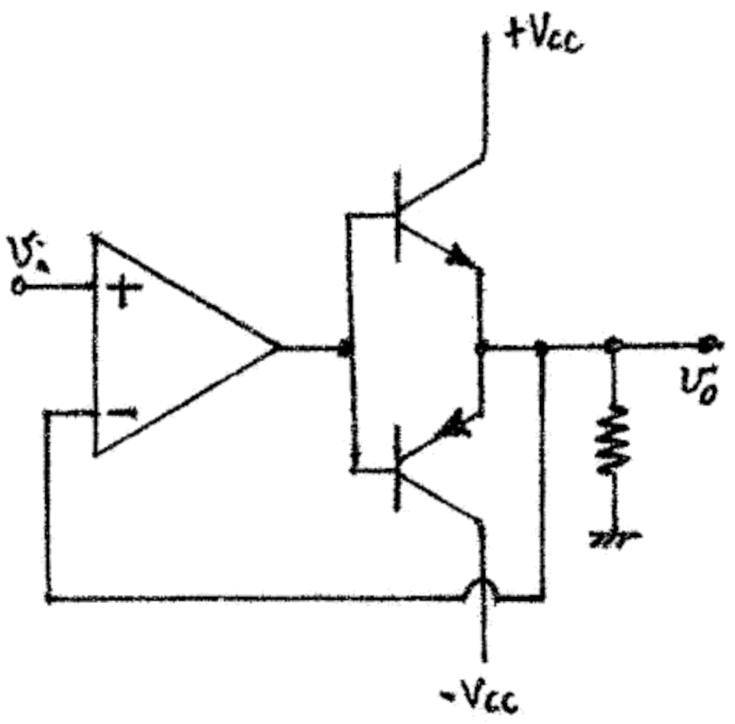
\includegraphics[width=0.38\linewidth]{_fig/multietapas_etapa-salida_polarizacion-retro.png}
		\label{fig:multietapas_etapa-salida_polarizacion-retro}
	}
	\caption{Polarización de Transistores}
	\label{fig:multietapas_etapa-salida_polarizacion}
\end{figure}

\subsection{Estructura interna de circuitos integrados} %109

En esta sección se analizará tres amplificadores construídos como circuitos integrados, el uA730, uA702 y el uA741, de diferentes grados de complejidad y sofisticación.

\subsubsection{El A730}

En la Figura \ref{fig:multietapas_estructura-interna-ic_a730}, se muestra la estructura interna de un circuito integrado sencillo, el A730, y a continuación las características principales dadas por el fabricante.

\begin{figure}[h]
	\centering
	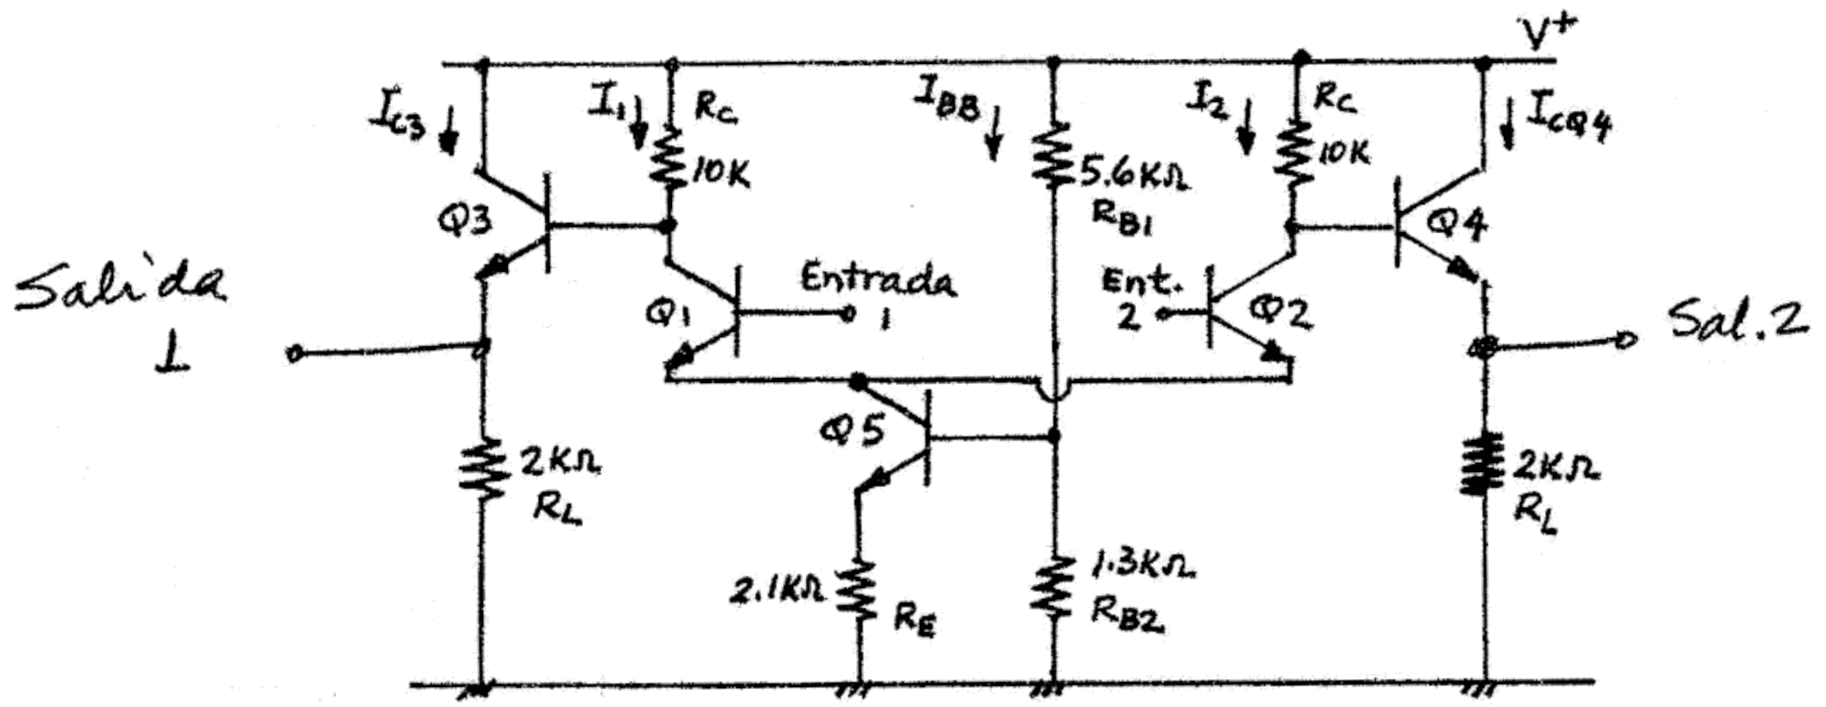
\includegraphics[width=0.8\linewidth]{_fig/multietapas_estructura-interna-ic_a730.png}
	\caption{Estructura interna del A730}
	\label{fig:multietapas_estructura-interna-ic_a730}
\end{figure}

\begin{itemize}
	\item Offset Voltaje: \( 1 \text{mV (max)} \)
	\item Offset Corriente: \( 0.5 \mu \text{A (max)} \)
	\item Corriente de Polarización: \( 3.5 \mu A \)
	\item Rango de Modo Común: \( 2.5 -> 4.5 \)
	\item Rango de Modo Diferencial: \( \pm 5V \)
	\item Ganancia de voltaje: \( 100 \)
	\item Ancho de banda: \( 1.5 \text{MHz} \)
	\item Voltage de suministro: \( 6V < V+ < 14V \), \( V+(tip)=12V \)
	\item CMRR = \( 85 dB \)
	\item Ri = \( 5K\Omega a 20K\Omega \)
\end{itemize}

Se hace notar que el circuito tiene una entrada diferencial y además una salida diferencial, cuyo símbolo se muestra en la Figura \ref{fig:multietapas_estructura-interna-ic_a730-simbolo}. En el circuito, $Q_5$ trabaja como una fuente de corriente, que polariza al par diferencial $Q_1$-$Q_2$, que a su vez impulsan el par diferencial $Q_3$-$Q_4$.

\begin{figure}[h]
	\centering
	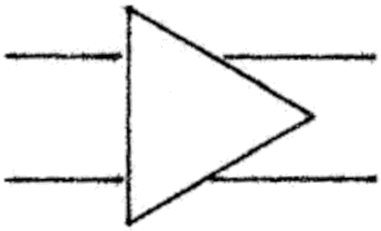
\includegraphics[width=0.3\linewidth]{_fig/multietapas_estructura-interna-ic_a730-simbolo.png}
	\caption{Estructura interna del A730}
	\label{fig:multietapas_estructura-interna-ic_a730-simbolo}
\end{figure}

Con \( V^+ = 12V \) y \( h_{fe} = 150 \), en la base de \( Q_5 \) queda el circuito planteado en la Figura \ref{fig:multietapas_estructura-interna-ic_a730} con su equivalencia de Thevenin, donde \( I_{B5} = 5.26\mu A \) e \( I = 798\mu A \). En equilibrio las corrientes de colector de \( Q_1 \) y \( Q_2 \) son iguales con valor igual a la mitad de \( I \), es decir \( 395\mu A \); por lo tanto se determina una caída en la resistencia de \( 10K\Omega \) de \( 3.95 V \). La corriente de base de estos transistores será: \( \frac{395\mu A}{150} = 2.63\mu A \), y está dentro del límite de \( 3.5\mu A \) máximo especificado por el fabricante. La caída máxima en \( R_C = 10K\Omega \) será \( 7.9V \).

Un extremo del \textbf{rango de modo común} viene dado por la exigencia de que la fuente de corriente permanezca en la región activa. Si el nivel de modo común de las entradas es muy bajo, el transistor \( Q_5 \) saldrá de la región activa (ver Figura \ref{fig:multietapas_estructura-interna-ic_a730-calculo-i}). El nivel mínimo ocurre para el voltaje colector-emisor de \( Q_5 \) apenas superior a saturación, y nos surge la siguiente ecuación:

\begin{figure}[h]
	\centering
	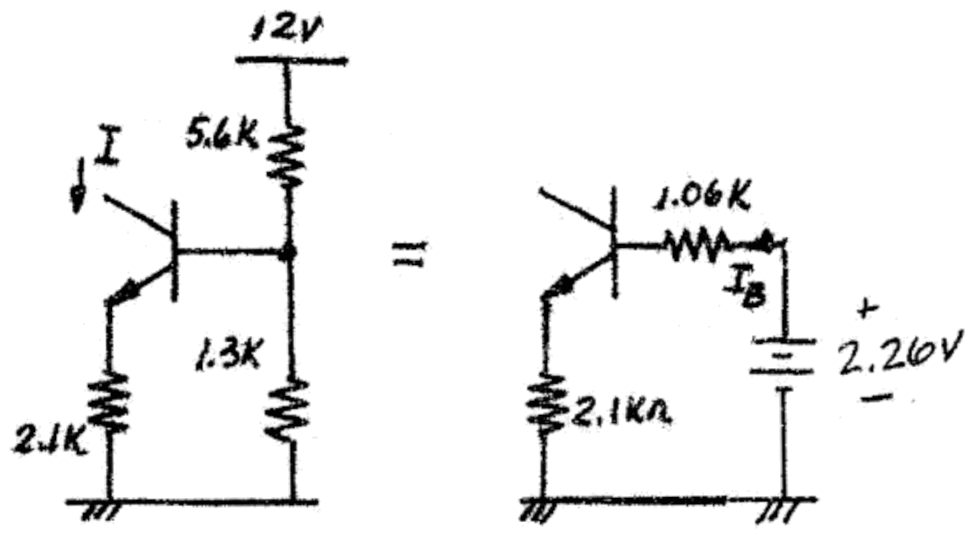
\includegraphics[width=0.3\linewidth]{_fig/multietapas_estructura-interna-ic_a730-calculo-i.png}
	\caption{Calculo del valor de corriente de la fuente de corriente}
	\label{fig:multietapas_estructura-interna-ic_a730-calculo-i}
\end{figure}

\[
V_{A(min)} \geq V_{BE R1} + V_{CE5 (sat)} + V_{E5} = 0.65 + 0.2 + 1.66 = 2.51V
\]

El nivel de modo común máximo viene limitado por la exigencia de que los transistores \( Q_1 \) y \( Q_2 \) admitan las máximas variaciones de la señal de colector sin salir de la región activa. Por lo tanto, surge la siguiente ecuación:

\[
V^+ - I_C R_C - \Delta V_{MAX} - V_{CE(sat)} + 0.6 = 12 - 3.95V - 3.95V - 0.2 + 0.6 = 4.5V
\]

La ganancia de voltaje diferencial a una salida sencilla viene dada por:

\[
G_v = -\frac{\beta R_C}{2r_\pi} \approx -76
\]

Para un amplificador diferencial, la resistencia de entrada viene dada por \( R_i = 2 r_{\pi} \); en este caso

\[
R_i = 2 (r_b + r_{\pi}) = 2 (r_b + 150 V_T / I_C)
\]

\[
R_i = 2 (r_b + 150 \times 26mV / 0.395mA) \approx 20K\Omega
\]

la resistencia de salida viene dada por:

\[
R_o = R_L // \left( \frac{R_C + r_{\pi}}{\beta + 1} \right) \approx 2K // \frac{10K + 10K}{151} \approx 125\Omega
\]

Podemos estimar la corriente total entregada por la fuente de poder, y por lo tanto la potencia disipada bajo condiciones de reposo. La corriente total entregada al circuito de la fuente de poder es:

\[
I_{CC} = I_C3 + I_1 + I_{BQ5} + I_2 + I_{CQ4} = 2(I_C3 + I_1) + I_{B5}
\]

donde: \( I_1 = 395\mu A\), \( I_{B5}(nom) = \frac{12V}{7.9V} = 1.5mA \), \( I_{C3} = \frac{(12 - 3.95 - 0.6)}{2K} = 3.73mA \) 

luego, \( I_{CC} = 12mA \) y la potencia nominal disipada: \( P_{MAX} = 12mA \times 12V = 144mW \)

\subsubsection{El uA702}

A continuación se trata la estructura interna del uA702 y sus características eléctricas principales (ver Figura \ref{fig:multietapas_estructura-interna-ic_ua702}).

\begin{figure}[h]
	\centering
	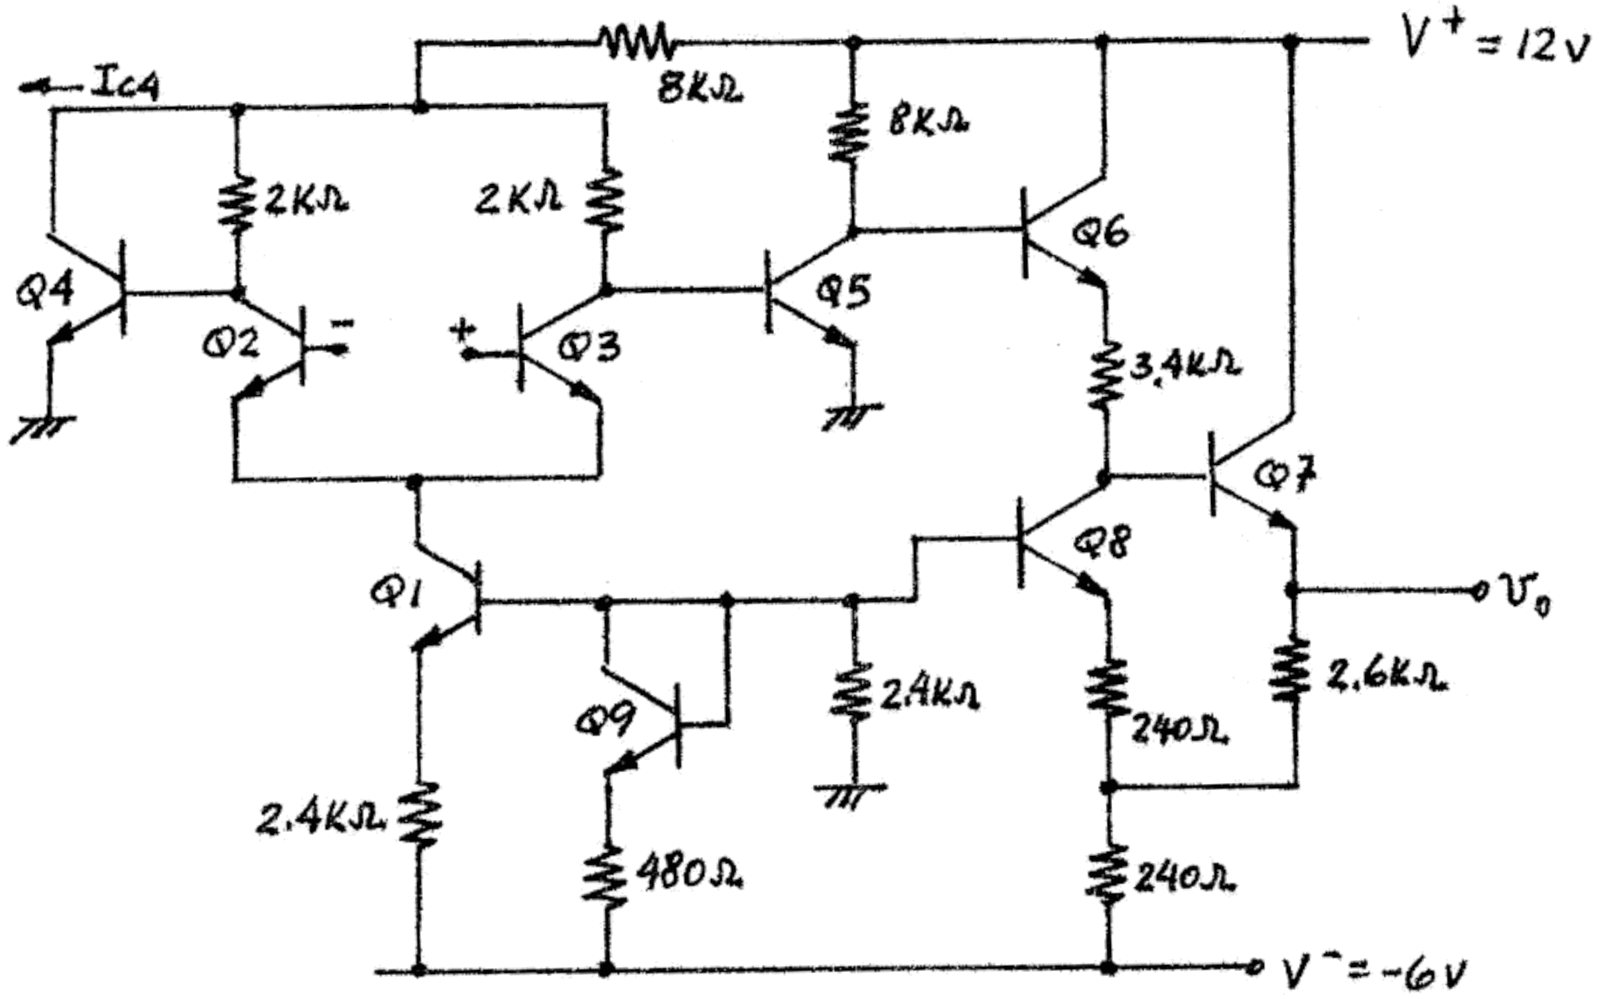
\includegraphics[width=0.8\linewidth]{_fig/multietapas_estructura-interna-ic_ua702.png}
	\caption{Estructura interna del uA702}
	\label{fig:multietapas_estructura-interna-ic_ua702}
\end{figure}

Caracteristicas Eléctricas: ( \( T_A = 25\circ C \), \( V^+ = 12V \), \( V^- = -6V \) )

\begin{table}[h]
	\centering
	\begin{tabular}{|l|c|c|c|c|c|}
		\hline
		\textbf{Parámetros} & \textbf{Condiciones} & \textbf{Min} & \textbf{Típico} & \textbf{Max} & \textbf{Unidad} \\
		\hline
		Voltaje Offset & $R_s < 2K\Omega$ & & 0.5 & 2 & mV \\
		Corriente Offset & & & 180 & 500 & nA \\
		Corr. Polarización & & & 2 & 5 & $\mu$A \\
		$R_{Entrada}$ &  & 16 & 40 &  & K$\Omega$ \\
		Rango Volt. In &  & -4 & & 0.5 & V \\
		CMRR & $R_s < 12K\Omega, F<1KHz$ & 80 & 100 & & dB \\
		Ganancia & $R_L \geq 100K\Omega, V_o = \pm5V$ & 2500 & 3600 & 6000 &  \\
		$R_{Salida}$ &  & 200 & 500 & & $\Omega$ \\
		Corriente Fuente & $V_o = 0$ & & 5.0 & 6.7 & mA \\
		Disipación Potencia & $V_o = 0$ & & 90 & 120 & mW \\
		\hline
	\end{tabular}
	\caption{Características Eléctricas}
\end{table}

El análisis se inicia con los niveles de señal en la condición de reposo.

La corriente que circula por las resistencias de base de Q9 es \( 1.88 mA \), el voltaje en la base de Q1 es \( -4.5V \) (la función de Q9 es la de compensar térmicamente el $V_{BE}$ de Q1); el voltaje a través de la resistencia de emisor de Q1 es \( 0.6V \), lo cual da una corriente de \( 375 \mu A \). 

Bajo condiciones de equilibrio, la corriente de colector de Q2 y Q3 es \( 188 \mu A \). La corriente por la resistencia de 8K es \( 375 \mu A + I_{C4} \) y el voltaje en el colector de Q3 es \( V_{BEQ5} \) es decir \( 0.6 V \). Entonces:

\[
(375\mu A + I_{C4}) \cdot 8K = 12 - (188\mu A) \cdot 2K - 0.6V
\]

de donde, \( I_{C4} = 1mA \). Dado que Q5 tiene un circuito de polarización idéntico a Q4, la corriente de colector de Q5 es igual a la corriente de colector de Q4, o sea \( I_{C5} = I_{C4} = 1mA \). Entonces, \( V_{CEQ5} = 12 - 8 \times 1mA = 4V \).

Para determinar los valores restantes se plantean las siguientes ecuaciones:

\begin{equation}
	I_{C8} \times 3.4K + V_{BEQ7} + I_{C7} \times 248 + (I_{C8} + I_{C7}) \times 248 - 6V = 3.4V
\end{equation}

\begin{equation}
	I_{C8} \times 3.4K + 0.6V + I_{C7} \times 2.6K + (I_{C8} + I_{C7}) \times 248 - 6V = 3.4V
\end{equation}

\begin{equation}
	I_{C8} \times 248 + (I_{C8} + I_{C7}) \times 248 - 6 = -4.5 - 0.6
\end{equation}

Despejando queda \( I_{C7} = 1.9mA \), \( I_{C8} = 920\mu A \) y \( V_o \approx 0.3V \).

Se hace notar que el voltaje de salida es casi \( 0 \); probablemente, si se hace el cálculo con otro valor de \( V_{BE} \), \( V_o \) se aproxima a \( 0V \).

El circuito formado por Q6, Q7 y Q8 es una configuración especial que suministra una ganancia de voltaje, una alta impedancia de entrada y una variación pico a pico del voltaje de salida que es casi igual a la diferencia entre los niveles de las fuentes de poder.

En la Figura \ref{fig:multietapas_estructura-interna-ic_ua702-conf-basica}, se traza la configuración básica:

\begin{figure}[h]
	\centering
	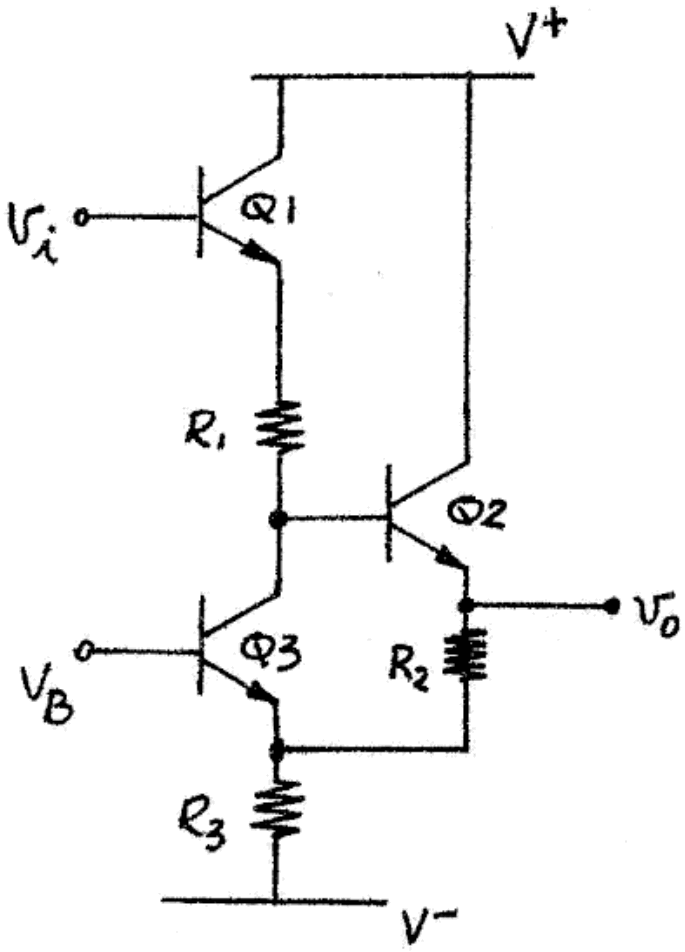
\includegraphics[width=0.4\linewidth]{_fig/multietapas_estructura-interna-ic_ua702-conf-basica.png}
	\caption{Configuración básica}
	\label{fig:multietapas_estructura-interna-ic_ua702-conf-basica}
\end{figure}

Del circuito se tiene que:

\[
V_i = V_{BE1} + I_{C3} R_1 + V_{BE2} + V_o
\]

y para pequeñas variaciones:

\[
V_i + \Delta V_i = V_{BE1} + (I_{C3} + \Delta I_{C3}) R_1 + V_{BE2} + V_o + \Delta V_o
\]

de donde: \( \Delta V_i = \Delta I_{C3} R_1 + \Delta V_o \)

además,

\[
V_B = V_{BE3} + (I_{C3} + \Delta I_{C3} + I_{C2} + \Delta I_{C2}) R_3 - 6
\]

es decir, \( \Delta I_{C3} = -\Delta I_{C2} \)

también, \( \Delta V_o = \Delta I_{C2} R_2 = -\Delta I_{C3} R_2 \Rightarrow \Delta I_{C3} = -\frac{\Delta V_o}{R_2} \)

entonces, \( \Delta V_i = \Delta V_o \left(1 - \frac{R_1}{R_2} \right) \)

y la ganancia, \( \frac{\Delta V_o}{\Delta V_i} = \frac{1}{1 - R_1/R_2} \)

Aplicado al circuito de salida del uA702 se consigue:

\( \Delta V_i = \Delta I_{C8} \times 3.4K + \Delta V_o \)

\( V_B = V_{BE3} + I_{C8} \times 248 + (I_{C8} + I_{C7}) \times 248 \)

\( \Delta I_{C8} = -\frac{\Delta I_{C2}}{2} \)

y, \( \Delta V_{in} = \Delta V_o \left(1 - \frac{3.4K}{5.48K} \right) \)

o

\begin{equation}
	\frac{\Delta V_o}{\Delta V_i} = 2.63
\end{equation}

\subsubsection{El uA741}

A continuación, en la Figura \ref{fig:multietapas_estructura-interna-ic_ua741}, se muestra el uA741, de uso muy extenso, que, a diferencia del uA739 y uA702, ha mantenido su popularidad durante muchos años.

\begin{figure}[h]
	\centering
	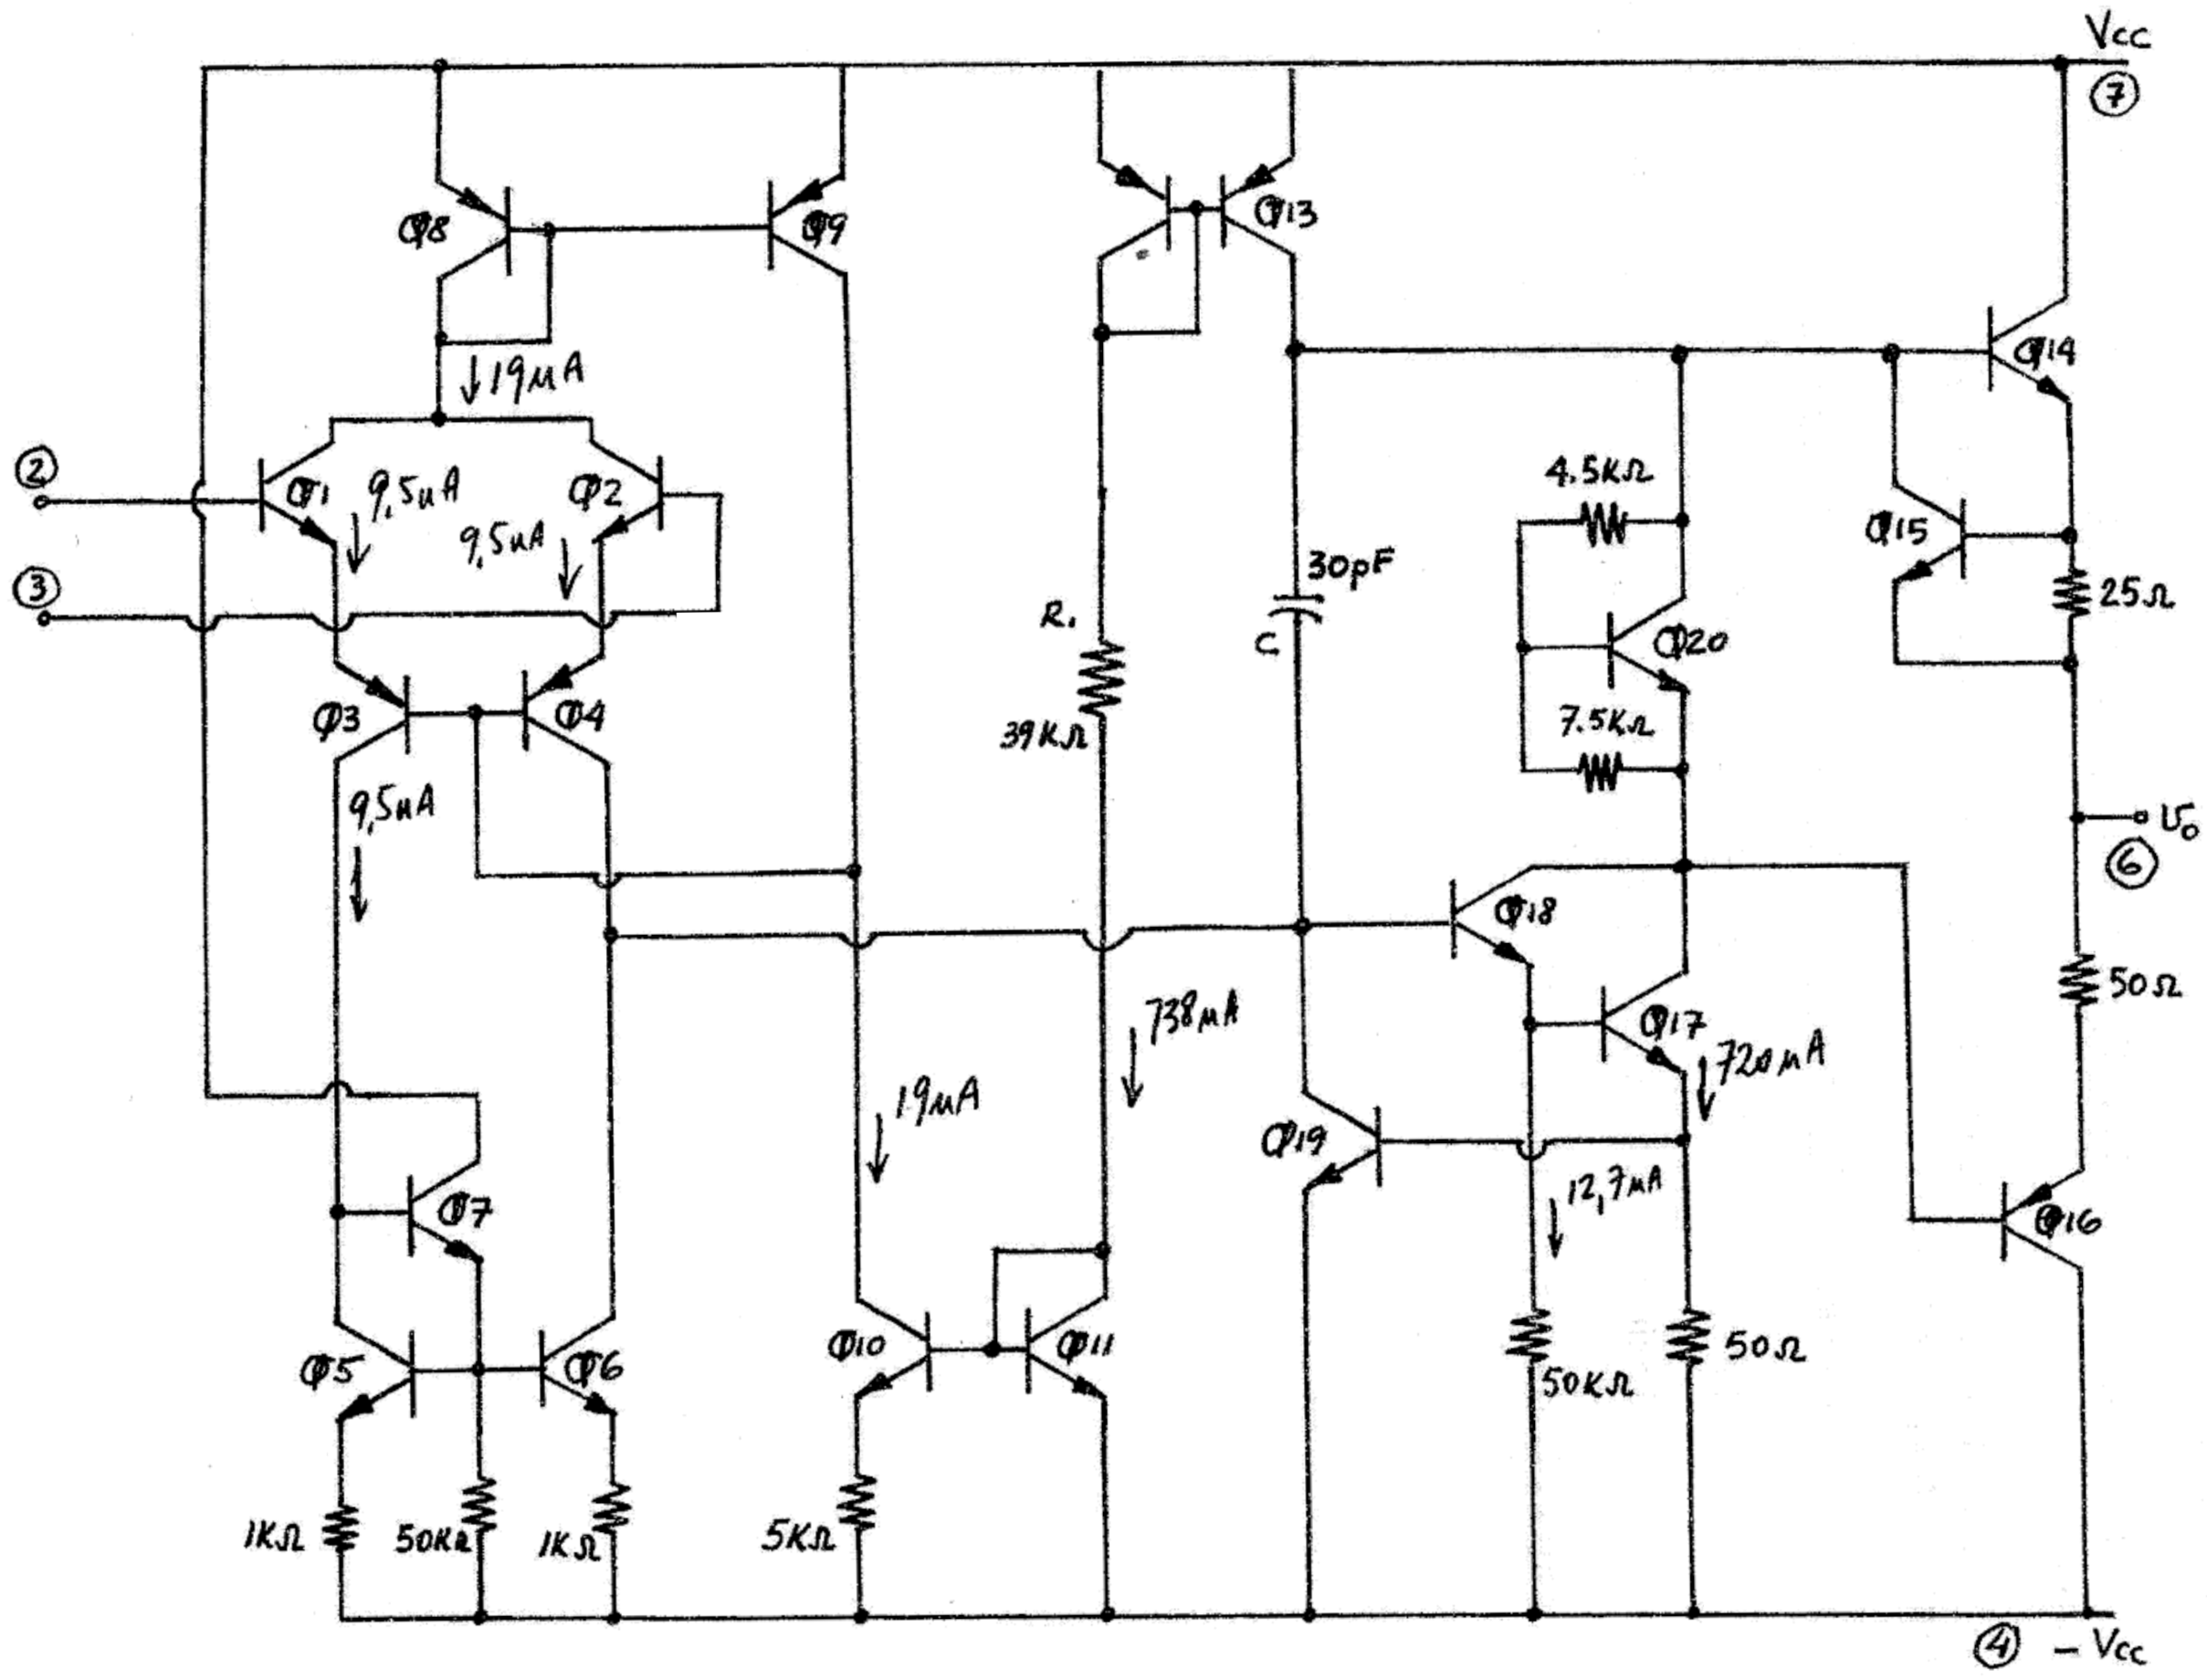
\includegraphics[width=0.8\linewidth]{_fig/multietapas_estructura-interna-ic_ua741.png}
	\caption{Estructura interna del uA702}
	\label{fig:multietapas_estructura-interna-ic_ua741}
\end{figure}

Sus mayores atractivos radican en el amplio rango de variación de los voltajes de entrada y salida, las protecciones y la compensación interna. Su mayor limitación es su ancho de banda.

Q1 y Q2 están en colector común, mientras que Q3 y Q4 están en base común. Estos cuatro transistores forman una etapa diferencial Cascode con una CMRR alta, $R_i$ alta y una ganancia diferencial del orden de \( 200 \). Q6 es la carga activa de Q4. Q5 y Q7 intervienen para polarizar Q6. Q10 y Q11 forman una fuente de baja corriente que suministra la corriente de polarización de base de Q3 y Q4 y una $I_C$ fija a Q9. Los transistores Q8 y Q9, junto con Q10 y Q11, fijan las corrientes de polarización para la etapa diferencial, de modo que: \( I_t = I_{C0} + I_{C1} + I_{C2} \). La interconexión de \(Q9\) con \(Q4\) y \(Q3\) en lazo cerrado ayuda a mantener \(I_{C1}\) e \(I_{C2}\) independientes de las variaciones de \(h_{fe}\).

La salida del amplificador diferencial alimenta al par Darlington \(Q18\) y \(Q17\) conectado como emisor común. \(Q13\) actúa tanto como carga activa para el par Darlington y como una fuente de corriente de polarización de \(Q20\) de manera que para señal cero una corriente de \(200\) \(\mu A\) circula por los transistores de salida.	\(Q12\) polariza a \(Q13\) y a través de la resistencia \(R_1\) suministra una corriente constante a \(Q11\). El amplificador Darlington tiene una ganancia de voltaje cercana a \(1000\) y excita a los amplificadores de salida, configurados como seguidores de emisor clase AB, formado por \(Q14\) y \(Q16\). El transistor \(Q20\) trabaja como un diodo Zener para dar la polarización apropiada entre las bases de \(Q14\) y \(Q16\).

Debido al efecto Miller, la capacitancia \(C\) se multiplica por la ganancia del par Darlington y crea así el polo dominante que hace el amplificador operacional estable.

Los transistores \(Q15\) y \(Q19\) forman la protección de cortocircuito. Normalmente están en corte debido a la poca caída de voltaje a través de \(R_2\) y \(R_3\) respectivamente. Cuando aumenta exorbitantemente la corriente por estas resistencias, el aumento en la caída de voltaje a través de ellas enciende a \(Q15\) o \(Q19\), desviando así la señal que impulsa la etapa de salida. La corriente de salida se limita a \( \frac{V_{BE}}{R_2} \), es decir, aproximadamente \( 25 \text{mA} \).

\section{Problemario} %p119
- pendiente en apuntes -	% Amplificadores de varias etapas
	% Licencia y derechos: consulte ../../LICENSE-CC-BY-4.0.
% Las figuras y demás materiales de terceros pueden tener derechos separados y deben identificarse.

\chapter{Retroalimentación} %p129
\section{Introducción} %p129

Una de las desventajas mayores de los componentes electrónicos es su sensibilidad a la temperatura y la dificultad de fabricar unidades que se reproduzcan exactamente igual, lo cual hace variable las características de los mismos.

Por medio de la retroalimentación vamos a crear sistemas cuyas características globales sean inmunes a la variabilidad de los valores de los elementos electrónicos. En particular, vamos a conseguir amplificadores cuya ganancia dependa solo de la relación de dos resistencias y podamos resistencias de entrada y salida tan pequeñas que las aproximemos a cero, o resistencias de entrada tan grandes que las aproximemos a infinito.

La retroalimentación tiene además los siguientes efectos:

\begin{itemize}
	\item Aumenta enormemente el ancho de banda del amplificador, bajando la frecuencia de corte baja y aumentando la frecuencia de corte alta en la misma proporción que disminuye la ganancia, conservándose así el producto ganancia-ancho de banda.
	\item Permite reducir enormemente ruido y distorsión producida interna en el amplificador.
\end{itemize}

\section{El lazo de retroalimnentación} %p129

En la Figura \ref{fig:retro_estructura-general} se muestra la estructura básica de retroalimentación.

\begin{figure}[h]
	\centering
	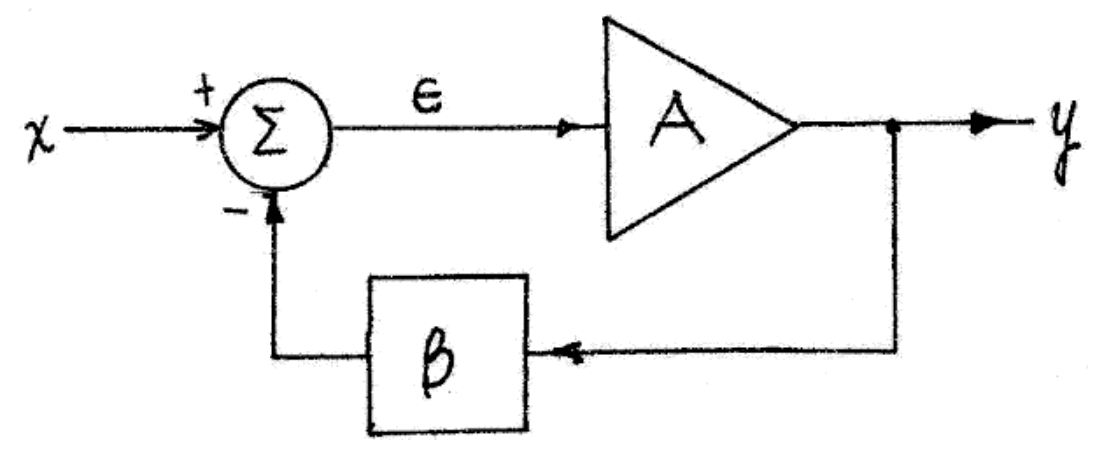
\includegraphics[width=0.9\linewidth]{_fig/retro_estructura-general.png}
	\caption{Estructura General de Retroalimentación}
	\label{fig:retro_estructura-general}
\end{figure}

Llamemos \( X \) a la señal de entrada, \( Y \) a la señal de salida, entonces se toma una muestra de la señal de salida, para retroalimentar una fracción, \( \beta Y \), a la entrada donde se compara con la señal de entrada genera así una diferencia \( e \). Esta diferencia es amplificada por \( A \) para generar la salida.

Entonces:

\[
e = x - \beta y
\]

\[
y = A e = A ( x - \beta y )
\]

\[
y + A \beta y = A x
\]

\[
y ( 1 + A \beta ) = A x
\]

\begin{equation}
	\frac{y}{x} = \frac{A}{1 + A \beta}
	\label{eq:retro1}
\end{equation}		

La ecuación \ref{eq:retro1} es la relación clásica de la retroalimentación. \( A \) generalmente representa un circuito activo con una relación muy elevada entre la salida y la entrada. \( \beta \) generalmente es un circuito pasivo. El producto \( A \beta \) tiene que ser adimensional. 

Si \( A \) y \( \beta \) son del mismo signo, el producto es positivo y corresponde a retroalimentación negativa. En cambio, si \( A \) y \( \beta \) son de signo contrario, se tiene retroalimentación positiva, lo que puede llevar a un sistema inestable.

Generalmente, \( A \beta \gg 1 \), de modo que:

\begin{equation}
	\frac{1}{1 + A \beta} \approx \frac{1}{A \beta}
	\label{eq:retro2}
\end{equation}

de aquí se destaca el mayor atributo de la retroalimentación en el sentido de que, en estas condiciones, la ganancia en el lazo cerrado, \( \frac{A}{1 + A \beta} \), es aproximadamente independiente de la ganancia en lazo abierto, \( A \), y depende únicamente de \( \beta \), que normalmente es un circuito pasivo, cuyas características son relarivamente invariables.

El efecto beneficioso sobre la distorsión o el ruido puede demostrarse por medio del diagrama de bloques, como el de la Figura \ref{fig:retro_estructura-general-ruido}, donde se ha introducido una señal de ruido \( n \).

\begin{figure}[h]
	\centering
	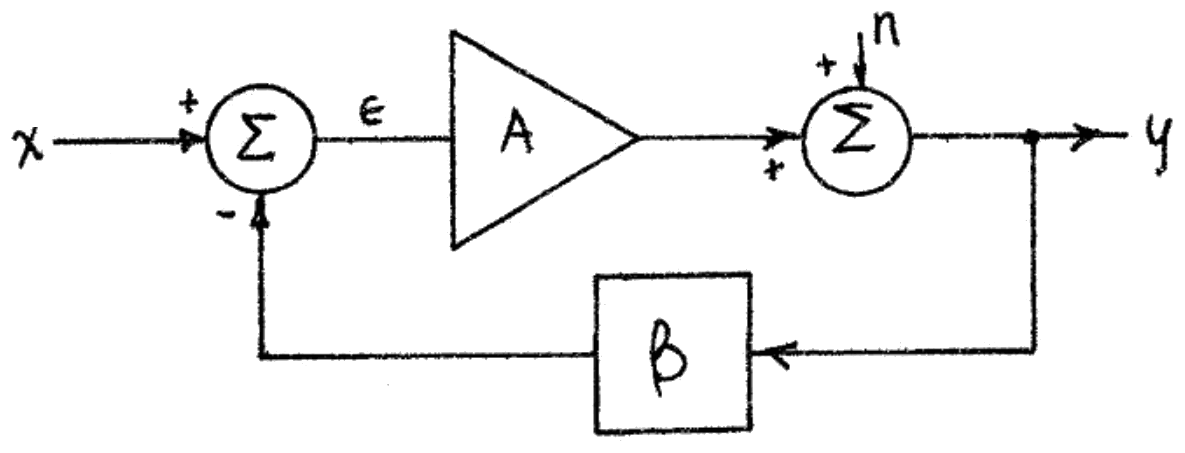
\includegraphics[width=0.9\linewidth]{_fig/retro_estructura-general-ruido.png}
	\caption{Sistema de Retroalimentación con Ruido}
	\label{fig:retro_estructura-general-ruido}
\end{figure}

Para hallar \( y \) en este caso aplicamos superposición, de donde:

\[
x_x = Ax(1 + A \beta)
\]

Para \( y_n \), se tiene:

\[
e = - \beta y_n
\]

\[
y_n = n + (-A \beta) y_n
\]

\[
y_n (1 + A \beta) = n
\]

\begin{equation}
	y_n = \frac{n}{1 + A \beta}
\end{equation}

es decir, a pesar el ruido se ha introducido en la misma puerta de salida, pero su componente en \( y_n \) se ve reducido por el factor \( 1 / (1 + A \beta) \).

\section{Análisis de los sistemas retroalimentados con métodos clásicos} %p131

A continuación, vamos a ver circuitos conocidos para demostrar cómo la retroalimentación puede tener los siguientes efectos:

\begin{itemize}
	\item - Aumenta el ancho de banda.
	\item Reduce la resistencia de entrada en algunos casos y la aumenta en otros.
	\item Reduce la resistencia de salida en algunos casos y la aumenta en otros.
\end{itemize}

Muchos de los circuitos que hemos visto han sido circuitos con retroalimentación, como por ejemplo, las configuraciones con Amplificador Operacional de la Figura \ref{fig:retro_gain}. La resistencia \( R_2 \) establece una comunicación de la salida con la entrada.

\begin{figure}[h]
	\centering
	\subfloat[Ganancia Negativa]
	{
		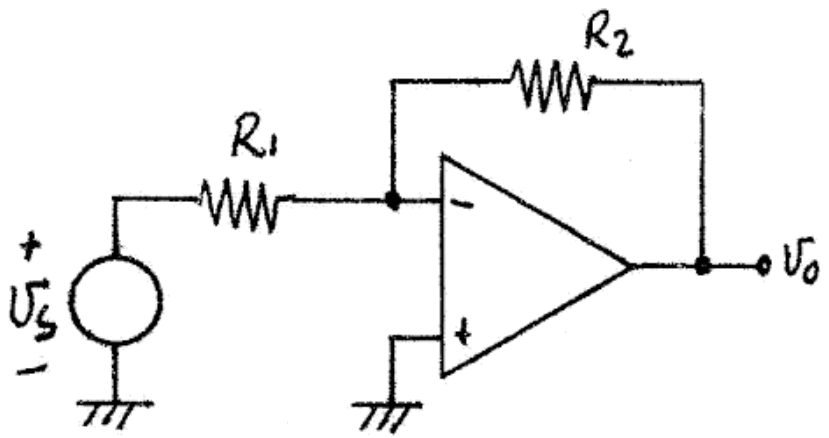
\includegraphics[width=0.4\linewidth]{_fig/retro_gain-neg.png}
		\label{fig:retro_gain-neg}
	}
	\subfloat[Ganancia Positiva]
	{
		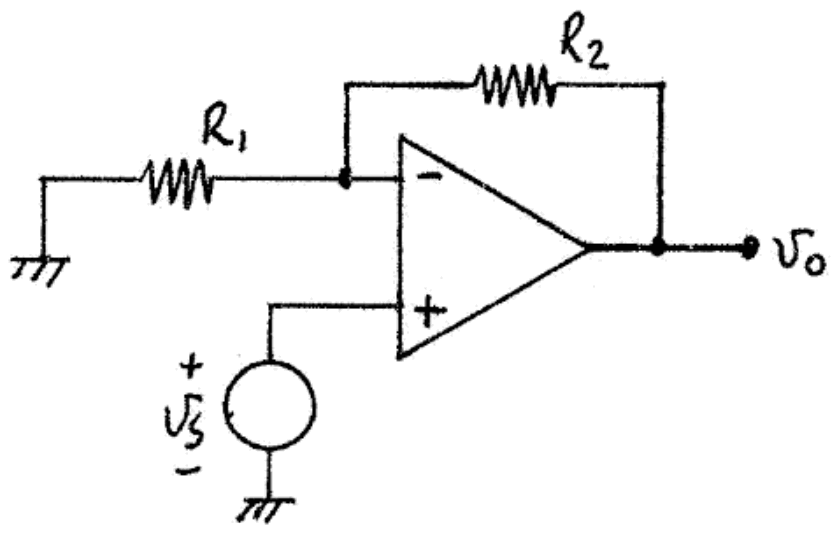
\includegraphics[width=0.4\linewidth]{_fig/retro_gain-pos.png}
		\label{fig:retro_gain-pos}
	}
	\caption{Amplificadores con Amplificador Operacional}
	\label{fig:retro_gain}
\end{figure}

\begin{figure}[h]
	\centering
	\subfloat[Modelo]
	{
		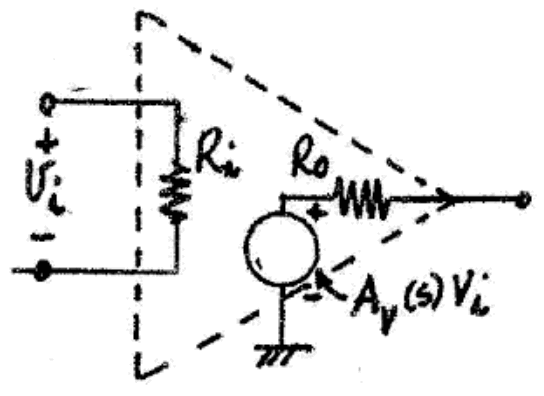
\includegraphics[width=0.4\linewidth]{_fig/retro_741-model.png}
		\label{fig:retro_741-model}
	}
	\subfloat[Respuesta de frecuencia]
	{
		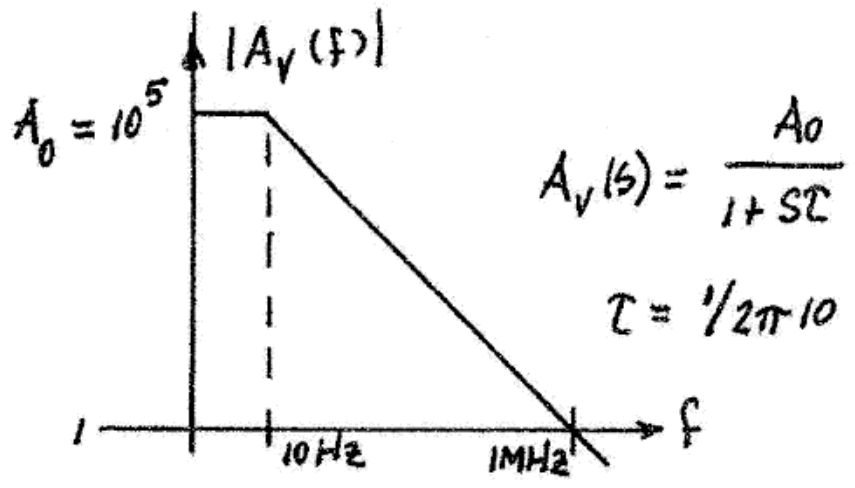
\includegraphics[width=0.4\linewidth]{_fig/retro_741-resp.png}
		\label{fig:retro_741-resp}
	}
	\caption{Modelo de un Amplificador Operacional con su Respuesta de Frecuencia}
	\label{fig:retro_741}
\end{figure}

Analicemos de nuevo estos circuitos. En la Figura \ref{fig:retro_741} se muestra el modelo a utilizar del amplificador operacional. Como valores para los elementos utilizamos las características del \textbf{uA741}, es decir:

\begin{itemize}
	\item Ganancia en lazo abierto de \( 100k \) (\( A_{vo} \)).
	\item Ancho de banda de \( 10 \) Hz (\( f_H = \frac{1}{2\pi \tau} \)).
	\item Resistencia de entrada de \( 6 M \Omega (R_i) \).
	\item Resistencia de salida de \( 25 M \Omega (R_o) \).
\end{itemize}

Veamos primero el efecto del ancho de banda con el circuito de la Figura \ref{fig:retro_741-model}. Para el modelo del operacional, consideramos su respuesta de frecuencia limitada, pero despreciamos por ahora el efecto que puede tener la resistencia de entrada y la resistencia de salida nos deja con el circuito equivalente de la Figura \ref{fig:retro_opamp-equiv}.

\begin{figure}[h]
	\centering
	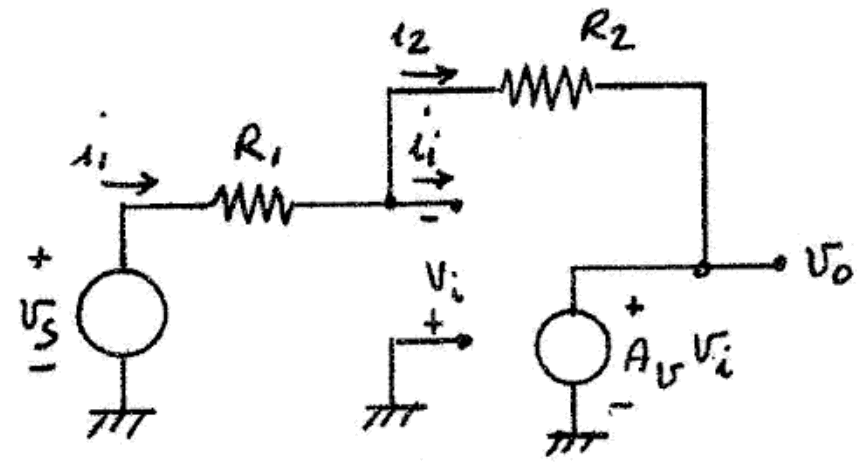
\includegraphics[width=0.9\linewidth]{_fig/retro_opamp-equiv.png}
	\caption{OpAmp Circuito Equivalente}
	\label{fig:retro_opamp-equiv}
\end{figure}

A la entrada se tiene:

\[
-v_i = \frac{-v_o}{A_v}
\]

Entonces,

\[
i_1 = \frac{v_s - (-v_o / A_v)}{R_1}
\]

\[
= \frac{v_s + v_o / A_v}{R_1}
\]

Aún consideramos \( R_i = \infty \) y \( R_o = 0 \). Entonces,

\[
i'_i = 0, \quad i_2 = i_1, \quad y \quad v_o = A_v v_i
\]

De modo que,

\[
v_o = -v_i - i_2 R_2
\]

\[
= -v_i - \left( \frac{v_s + v_o / A_v}{R_1} \right) R_2
\]

\[
= \frac{-v_o}{A_v} - \frac{v_s R_2}{R_1} - (\frac{v_o}{A_v})(\frac{R_2}{R_1})
\]

De donde:

\begin{equation}
	\frac{v_o}{v_s} = \frac{-R_2 / R_1}{1 + (1 + R_2 / R_1) / A_v}
\end{equation}

Ahora reemplazamos \( A_v = A_{v0} (1 + j f / f_{a0}) \), nos queda:

\[
\frac{v_o}{v_s} = -\left(\frac{R_2}{R_1}\right) \left( \frac{1}{1 + (1 + R_2/R_1)(1 + j f / f_{a0}) / A_{v0}} \right)
\]

\[
= -\left(\frac{R_2}{R_1}\right) \frac{1}{1 + (1 + R_2/R_1)/A_{v0} + (1 + R_2/R_1) j f / f_{a0} A_{v0}}
\]

Si \( A_{v0} \gg 1 + R_2 / R_1 \), y despreciamos ese término, entonces nos queda:

\[
\frac{v_o}{v_s} \approx -\left(\frac{R_2}{R_1}\right) \frac{1}{1 + j f (1 + R_2/R_1) / A_{v0} f_{a0}}
\]

De donde se desprende que la frecuencia de corte de la configuración, \( f_{corte} \), el coeficiente de \( j f \), viene dado por:

\[
f_{corte} = \frac{A_{v0} f_{a0}}{(1 + R_2 / R_1)} = \frac{f_T}{(1 + R_2 / R_1)}
\]

De forma semejante, uno podría analizar la configuración del amplificador con ganancia positiva, y el análisis daría que la ganancia de DC es igual a \( 1 + R_2/R_1 \), y que la frecuencia de corte es igual a la expresión anterior.

\subsection{Ejemplo}

Considere un A.O. con \( f_{a0} = 1 \) MHz. Hallar la frecuencia de corte del amplificador en lazo cerrado con ganancias de \( +1000, +100, +10, +1, -1, -10, -100, -1000 \).

\subsubsection{Solución}

\begin{table}[h]
	\centering
	\begin{tabular}{|c|c|c|c|}
		\hline
		\textbf{Ganancia en lazo cerrado} & \( R_2 / R_1 \) & \( f_{corte} \) & \textbf{Prod. \( A_v \) x BW} \\
		\hline
		1000  & 999  & 1 kHz   & 1 MHz  \\
		100   & 99   & 10 kHz  & 1 MHz  \\
		10    & 9    & 100 kHz & 1 MHz  \\
		1     & 0    & 1 MHz   & 1 MHz  \\
		-1    & 1    & 0.5 MHz & 0.5 MHz \\
		-10   & 10   & 90.9 kHz & 0.9 MHz \\
		-100  & 100  & 9.9 kHz & 0.99 MHz \\
		-1000 & 1000 & 1 kHz   & 1 MHz  \\
		\hline
	\end{tabular}
	\caption{Frecuencia de corte y producto ganancia-ancho de banda para diferentes configuraciones}
\end{table}

En resumen, la ganancia disminuye y la frecuencia de corte alta aumenta con retroalimentación. Sobre la misma respuesta de frecuencia en lazo abierto del amplificador operacional (amplificador en lazo abierto), puede trazarse la respuesta del amplificador con retroalimentación, en la Figura \ref{fig:retro_741-resp-misc}, muestra que la frecuencia de corte con retroalimentación se encuentra como la intersección de la ganancia con retroalimentación con la característica sin retroalimentación.

\begin{figure}[h]
	\centering
	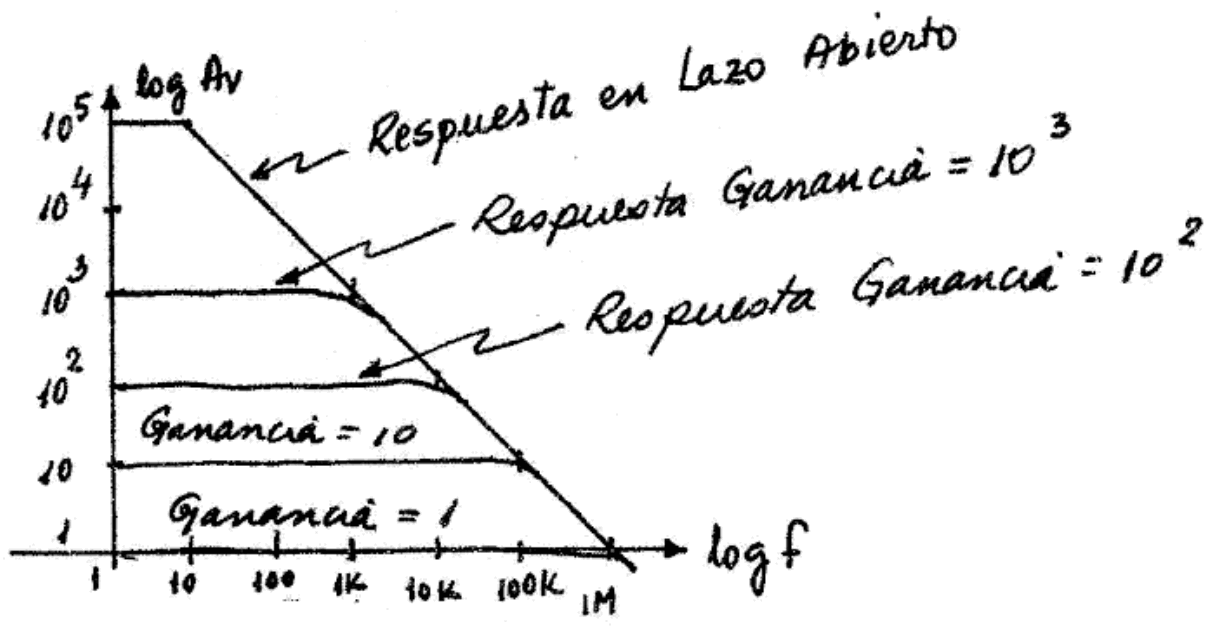
\includegraphics[width=0.9\linewidth]{_fig/retro_741-resp-misc.png}
	\caption{Respuesta en lazo abierto y con retroalimentación}
	\label{fig:retro_741-resp-misc}
\end{figure}

Consideramos ahora el efecto sobre la resistencia de entrada del mismo amplificador, tomando su \( R_i' \) en cuenta. Se muestra un circuito equivalente en la Figura \ref{fig:retro_741-with-retro}.

\begin{figure}[h]
	\centering
	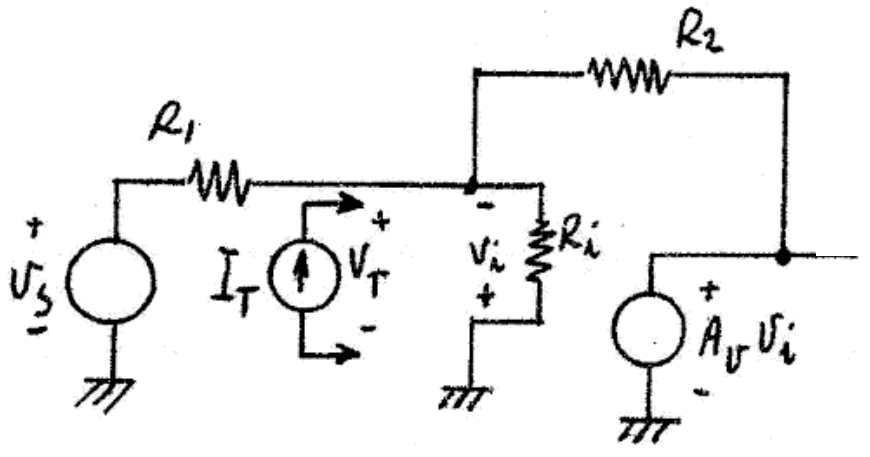
\includegraphics[width=0.9\linewidth]{_fig/retro_741-with-retro.png}
	\caption{Circuito equivalente con retroalimentación}
	\label{fig:retro_741-with-retro}
\end{figure}

Del circuito se obtiene:

\[
I_T + v_i / R_i' + (A_v v_i - (-v_i)) / R_2 = 0
\]

\[
I_T = - v_i \left( \frac{1}{R_i'} + \frac{(A_v + 1)}{R_2} \right)
\]

Pero \( -v_i = v_T \), entonces:

\[
\frac{v_T}{I_f} = \frac{1}{\left( \frac{1}{R_i'} + \frac{(A_v + 1)}{R_2} \right)}
\]

\[
= \frac{R_i'}{\left( \frac{R_2}{(A_v + 1)} \right)}
\]

Se ha reducido la gran \( R_i \) sin retroalimentación (\(6 M\Omega\) para el 741), a una \( R \) de entrada muy pequeña \( \approx 0.1 \Omega \) si \( R_2 = 10k\Omega \) y \(A_0 = 10^5 \); se ha aumentado la conductancia de entrada.

En cambio, para la configuración de ganancia positiva, que se muestra en la Figura \ref{fig:retro_conf-gain-pos}:

\[
v_i = I_T R_i
\]

\[
I_T = \frac{(E_T - v_i)}{R_1} + \frac{(E_T - v_i - A_v v_i)}{R_2}
\]

\begin{figure}[h]
	\centering
	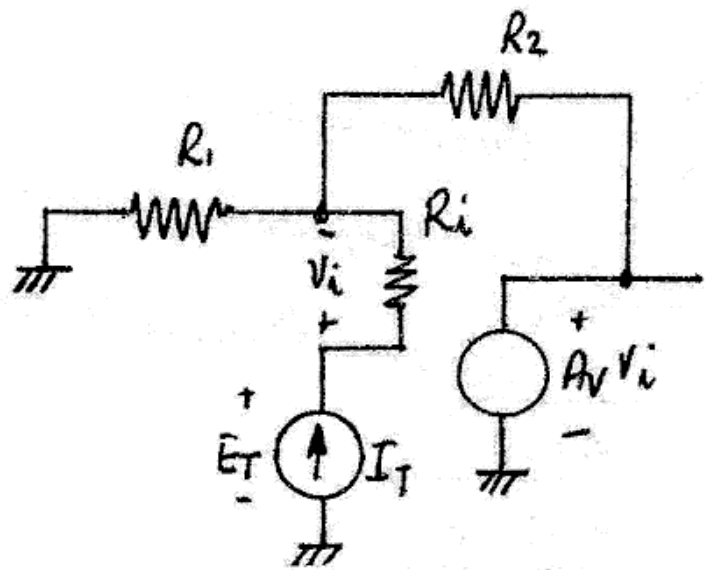
\includegraphics[width=0.7\linewidth]{_fig/retro_conf-gain-pos.png}
	\caption{Configuración de ganancia positiva}
	\label{fig:retro_conf-gain-pos}
\end{figure}

\[
I_T = E_T \left(\frac{1}{R_1} + \frac{1}{R_2} \right) - v_i \left(\frac{1}{R_1} + \frac{(1+A_v)}{R_2} \right)
\]

Luego,

\[
I_T \left(1 + R_i' \left(\frac{1}{R_1} + \frac{(1+A_v)}{R_2} \right) \right) = E_T \left(\frac{1}{R_1} + \frac{1}{R_2} \right)
\]

\[
R_{if} = \frac{E_T}{I_T} = R_1 \parallel R_2 \left(1 + R_i' \left(\frac{R_1}{R_2} + \frac{1+A_v}{R_2} \right) \right)
\]

Por ejemplo, si \( R_i = 6 M\Omega \), \( R_1 = 1 k\Omega \), \( R_2 = 10 k\Omega \), \( A_v = 10^5 \), nos da \( 54551 M\Omega \) (9091 veces mayor que \( R_i' \)).

Finalmente, determinemos \( R_{of} \) para el circuito de ganancia positiva o negativa. Nuevamente se considera \( A_v \) un valor limitado y por ahora consideramos \( R_f \) infinito. El circuito equivalente se muestra en la Figura \ref{fig:retro_calc-rof}.

\begin{figure}[h]
	\centering
	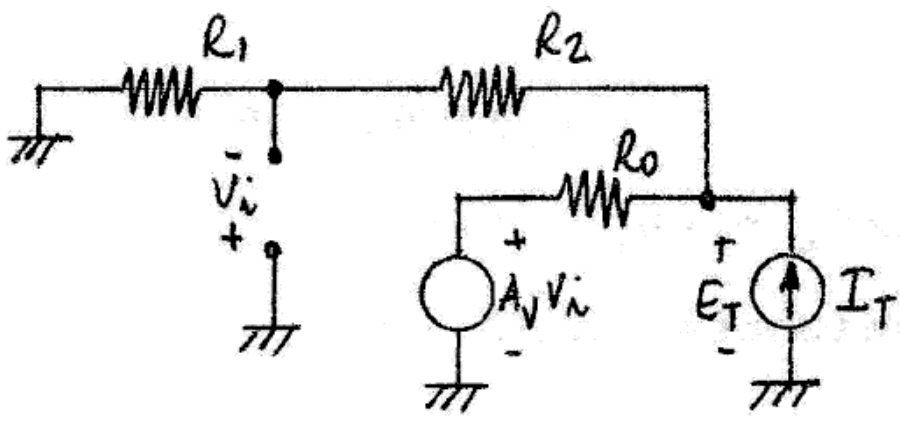
\includegraphics[width=0.9\linewidth]{_fig/retro_calc-rof.png}
	\caption{Circuito equivalente para determinar \( R_{of} \)}
	\label{fig:retro_calc-rof}
\end{figure}

Se tiene:

\[
I_T = \frac{(v_T - A_v v_i)}{R_0} + \frac{v_T}{(R_2 + R_1)}
\]

\[
- v_i = R_i V_T (R_1 + R_2)
\]

Entonces,

\[
I_T = V_T \left[ \left( \frac{1 + A_v R_i / (R_1 + R_2)}{R_0} \right) + \frac{1}{(R_1 + R_2)} \right]
\]

o

\[R_{of} = \frac{V_T}{I_T} = \frac{R_0}{(1 + A_v R_i / (R_1 + R_2))} \parallel (R_1 + R_2)
\]

\[
\approx \frac{R_0}{(1 + A_v R_i / (R_1 + R_2))}
\]

Ahora podemos utilizar valores finitos de \( R_0 \) y \( A_v \) para encontrar \( R_{of} \).

Si \( R_1 = 1k\Omega \), \( R_2 = 9k\Omega \), \( A_v = 100,000 \) y \( R_0 = 25\Omega \), da

\[
R_{of} \approx \frac{25}{(1 + 10^5 / 10)} \approx 25 \times 10^{-3} = 2.5 m\Omega
\]

Hemos demostrado los efectos de la retroalimentación sobre circuitos muy conocidos con herramientas también conocidas ("a pie").  
En las próximas secciones presentamos una metodología orientada especialmente a sistemas retroalimentados.  
Consiste en encontrar \( A \) y \( \beta \) por separado y utilizar el factor \( (1 + A\beta) \) para determinar la frecuencia de corte alta y baja, la resistencia de entrada y salida.  
De tal forma, se tendrá mayor intuición sobre por qué y cómo los sistemas retroalimentados consiguen su efecto, y de paso nos brindará una herramienta que frecuentemente será más eficaz para determinar las características del circuito.  

Por ahora hemos podido comprobar que la retroalimentación realmente tiene estos efectos.

\section{Cuatro configuraciones básicas con retroalimentación} %p137

La configuración básica con retroalimentación, la Figura 3.1, es una representación genérica de un sistema, de modo que los variables de entrada, salida y retroalimentación pueden ser cualquier parámetro, como por ejemplo, tensión, corriente, fase, frecuencia, etc. Por ahora, nuestro interés estará centrado en esos casos donde las variables son tensiones o corrientes. Para ellos:

\begin{enumerate}
	\item Si se muestrea la tensión de salida, Figura \ref{fig:retro_conf_muestreo-nodo}, entonces \( y = v \); esto se conoce como \textbf{muestreo de nodo} y tiene el efecto de reducir la resistencia del nodo de salida.
	\item En cambio, si se muestrea la corriente de salida, Figura \ref{fig:retro_conf_muestreo-lazo}, entonces \( y = i \); esto se conoce como \textbf{muestreo de lazo} y tiene el efecto de aumentar la resistencia del lazo de salida.
	\item Si se comparan tensiones a la entrada, Figura \ref{fig:retro_conf_comparacion-lazo}, entonces \( x = v \); esto se conoce como \textbf{comparación de lazo} y tiene el efecto de aumentar la resistencia del lazo de entrada.
	\item Finalmente, si se comparan corrientes a la entrada, Figura \ref{fig:retro_conf_comparacion-nodo}, entonces \( x = i \); esto se conoce como \textbf{comparación de nodo} y tiene el efecto de reducir la resistencia del nodo de entrada.
\end{enumerate}

\begin{figure}[h]
	\centering
	\subfloat[Muestreo de Nodo]
	{
		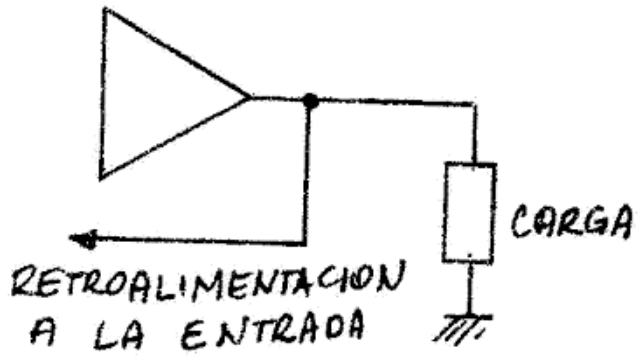
\includegraphics[width=0.22\linewidth]{_fig/retro_conf_muestreo-nodo.png}
		\label{fig:retro_conf_muestreo-nodo}
	}
	\subfloat[Muestreo de Lazo]
	{
		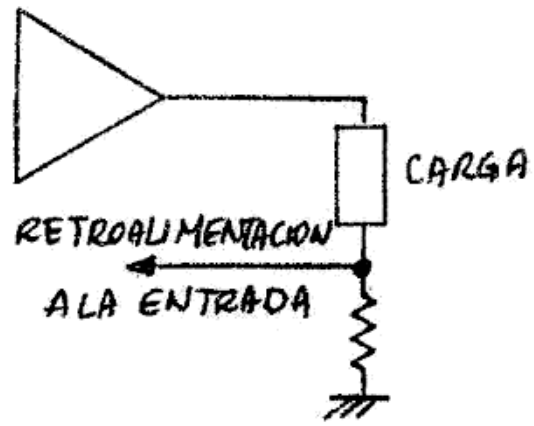
\includegraphics[width=0.22\linewidth]{_fig/retro_conf_muestreo-lazo.png}
		\label{fig:retro_conf_muestreo-lazo}
	}
	\subfloat[Comparación de Lazo]
	{
		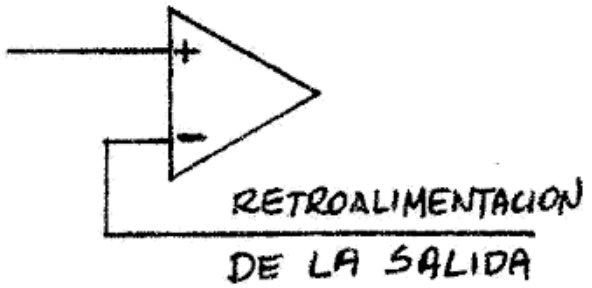
\includegraphics[width=0.22\linewidth]{_fig/retro_conf_comparacion-lazo.png}
		\label{fig:retro_conf_comparacion-lazo}
	}
	\subfloat[Comparación de Nodo]
	{
		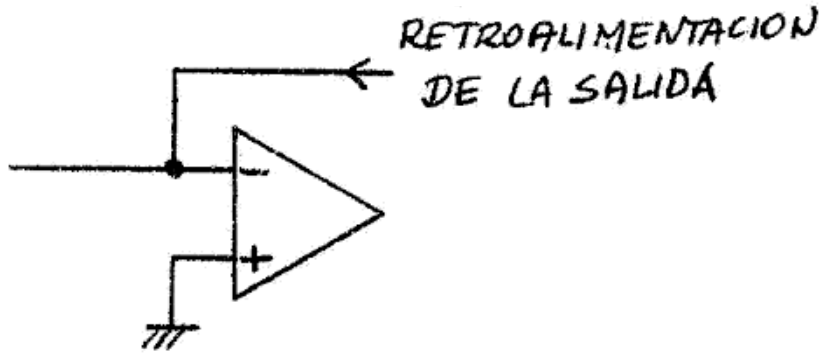
\includegraphics[width=0.22\linewidth]{_fig/retro_conf_comparacion-nodo.png}
		\label{fig:retro_conf_comparacion-nodo}
	}
	\caption{ Diagramas de tipos de muestreo y comparación}
	\label{fig:retro_conf}
\end{figure}

La combinación de uno de los dos tipos de muestreo a la combinación de uno de los dos tipos de comparación a la entrada da lugar a cuatro configuraciones de retroalimentación. En la Tabla 3.1 se hace un cuadro comparativo, donde se destaca el tipo de señal a la entrada y a la salida, el efecto sobre la resistencia de entrada y de salida, y el tipo de relación que resulta ser \(\beta\) y \(A\).

\begin{table}[h]
	\centering
	\begin{tabular}{|l|c|c|c|c|c|c|}
		\hline
		\textbf{Tipo de retroalimentación} & \textbf{S. \( y \)} & \textbf{S. \( x \)} & \( R_{of} \) & \( R_{if} \) & \( \beta \) & \( A \) \\
		\hline
		M. Nodo - Comp. de Lazo & \( v_o \) & \( v_s \) & dism. & aum. & \( v_f / v_o \) & \( v_o / v_s \) \\
		\hline
		M. Lazo - Comp. de Nodo & \( i_o \) & \( i_s \) & aum. & dism. & \( i_f / i_o \) & \( i_o / i_s \) \\
		\hline
		M. Nodo - Com[p.] de Nodo & \( v_o \) & \( i_s \) & dism. & dism. & \( i_f / v_o \) & \( v_o / i_s \) \\
		\hline
		M. Lazo - Comp. de Lazo & \( i_o \) & \( v_s \) & aum. & aum. & \( v_f / i_o \) & \( i_o / v_s \) \\
		\hline
	\end{tabular}
	\caption{Tabla 3.1. Cuadro Comparativo de los Tipos de Retroalimentación.}
	\label{tab:retro_comparativo}
\end{table}

A continuación, para cada tipo de retroalimentación vamos a mostrar tres figuras: en la primera, un esquema de interconexión de cuadripolos en su forma más general; en la segunda, un esquema de interconexión de cuadripolos más parecido a circuitos reales, donde se indican las conexiones a tierra; y finalmente, para cada tipo, un ejemplo de un circuito real, bien sea transistorizado o con amplificadores operacionales.

\subsection{Muestreo de Nodo - Comparación de Lazo} %p139

En la Figura \ref{fig:retro_m-nodo_c-lazo_a} se muestra el diagrama de bloques de este tipo de retroalimentación donde las señales de interés son las tensiones de salida y de entrada. La red \(\beta\) de retroalimentación devuelve una tensión \( v_f \) a la entrada que es una muestra de la tensión de salida \( v_o \); por lo tanto, \( \beta \) es una relación de tensiones.

En la Figura \ref{fig:retro_m-nodo_c-lazo_a} se muestra una comparación de lazo con muestreo de nodo.

\begin{figure}[h]
	\centering
	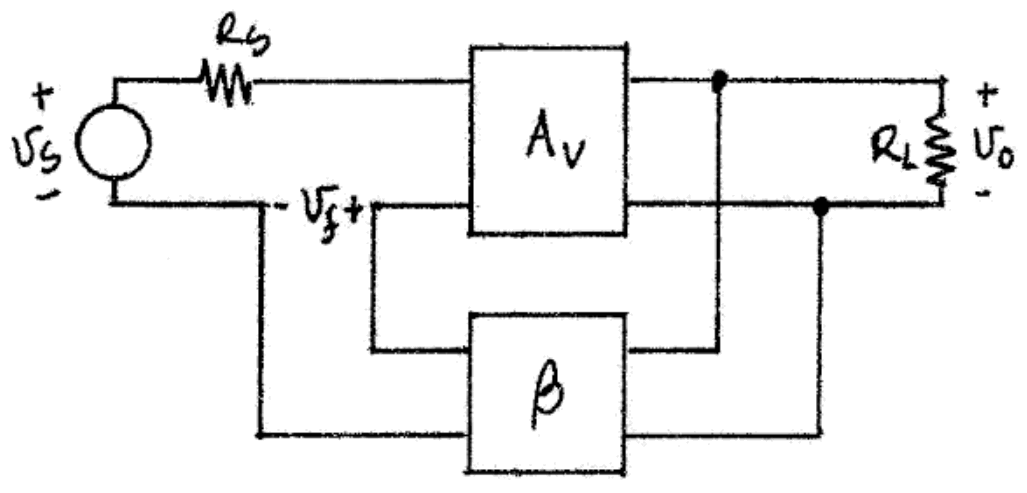
\includegraphics[width=0.6\linewidth]{_fig/retro_m-nodo_c-lazo_a.png}
	\caption{Muestreo de Nodo - Comparación de Lazo}
	\label{fig:retro_m-nodo_c-lazo_a}
\end{figure}

En la Figura \ref{fig:retro_m-nodo_c-lazo_b} se representa de nuevo este tipo de retroalimentación, pero ahora referenciando los cuadripolos a tierra. Además, se ha indicado dentro del bloque de \( \beta \) la configuración típica de esta como un divisor de tensión formado por dos resistencias.

\begin{figure}[h]
	\centering
	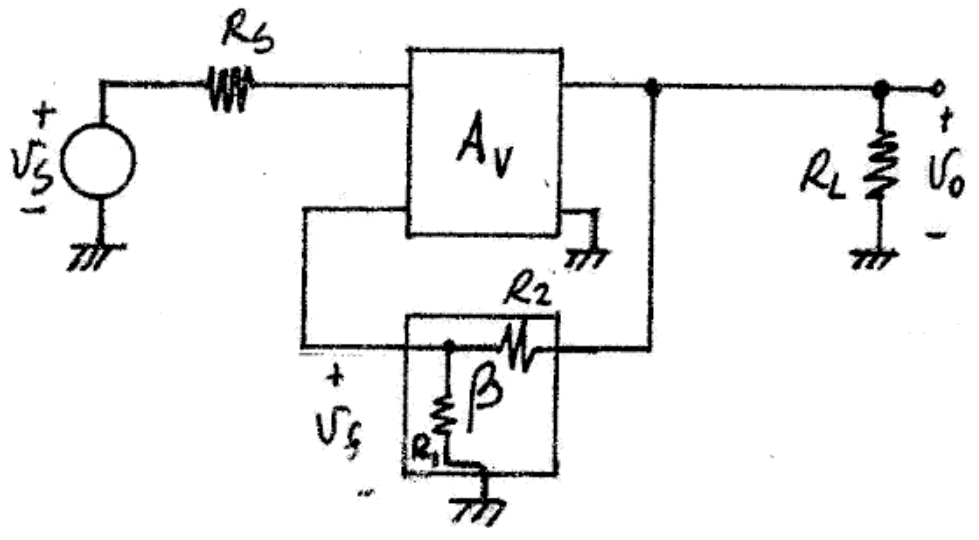
\includegraphics[width=0.6\linewidth]{_fig/retro_m-nodo_c-lazo_b.png}
	\caption{Muestreo de Nodo - Comparación de Lazo}
	\label{fig:retro_m-nodo_c-lazo_b}
\end{figure}

En la Figura \ref{fig:retro_m-nodo_c-lazo_c} se muestran dos ejemplos de circuitos con este tipo de retroalimentación.

\begin{figure}[h]
	\centering
	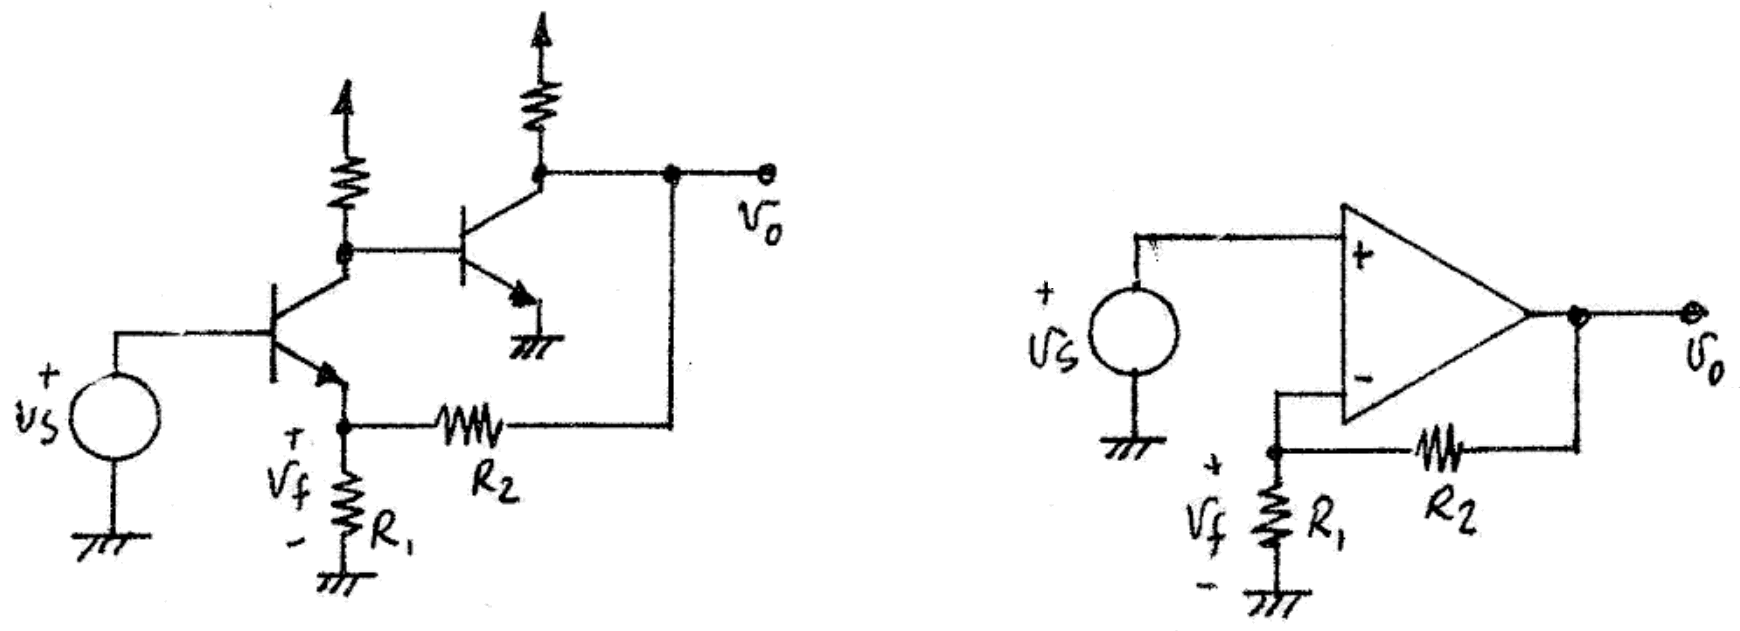
\includegraphics[width=0.8\linewidth]{_fig/retro_m-nodo_c-lazo_c.png}
	\caption{Muestreo de Nodo - Comparación de Lazo}
	\label{fig:retro_m-nodo_c-lazo_c}
\end{figure}

\subsection{Muestreo de Lazo - Comparación de Nodo} %p141

En la Figura \ref{fig:retro_m-lazo_c-nodo_a} se muestra el diagrama de bloques de este tipo de retroalimentación, donde las señales de interés son las corrientes de salida y de entrada. La red $\beta$ de retroalimentación devuelve una corriente $i_f$ a la entrada, que es una muestra de la corriente de salida $i_o$; Por lo tanto, $\beta$ es una relación de corrientes. A su vez, el bloque $A_I$ representa un amplificador de corrientes.

\begin{figure}[h]
	\centering
	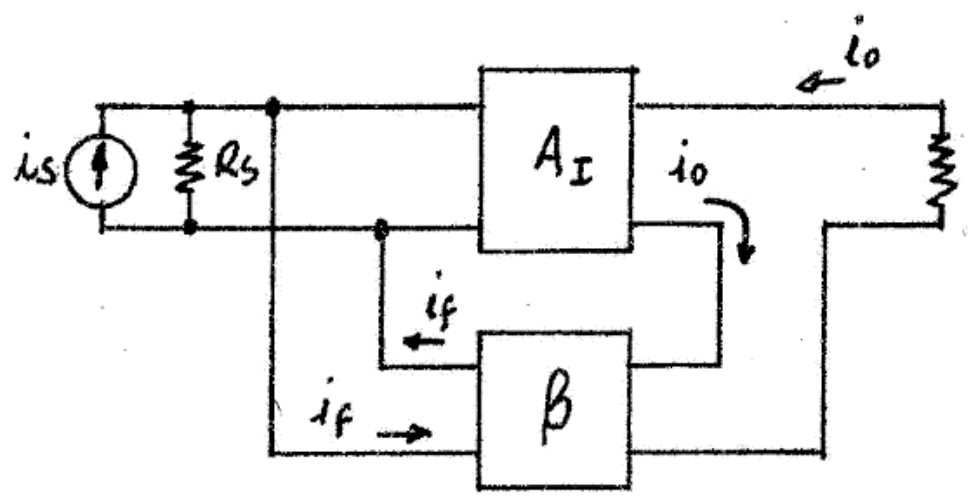
\includegraphics[width=0.6\linewidth]{_fig/retro_m-lazo_c-nodo_a.png}
	\caption{Muestreo de Lazo - Comparación de Nodo}
	\label{fig:retro_m-lazo_c-nodo_a}
\end{figure}

En la Figura \ref{fig:retro_m-lazo_c-nodo_b} se representa de nuevo este tipo de retroalimentación, pero ahora referenciando los cuadripolos a tierra. Además, se ha indicado dentro del bloque de $\beta$ la configuración típica de esta como un divisor de corriente formado por dos resistencias.

\begin{figure}[h]
	\centering
	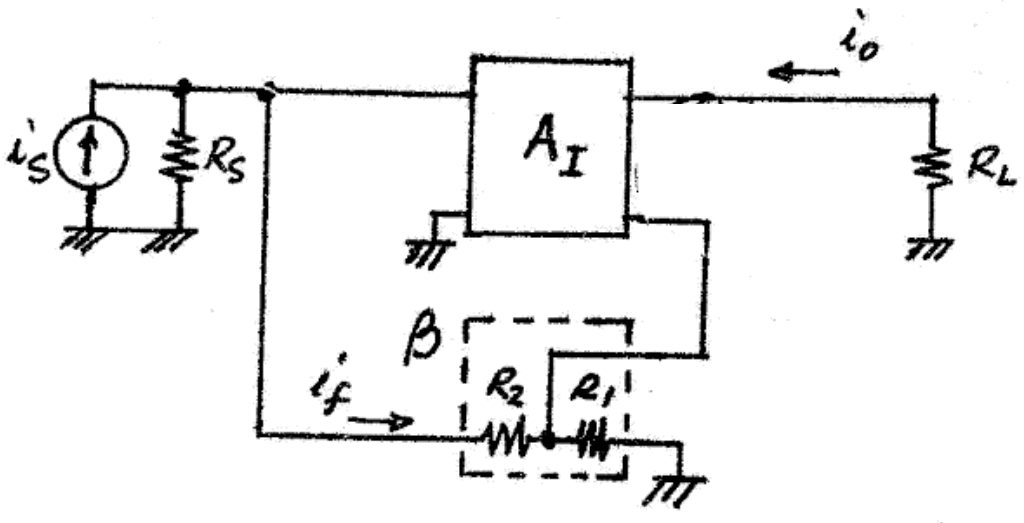
\includegraphics[width=0.6\linewidth]{_fig/retro_m-lazo_c-nodo_b.png}
	\caption{Muestreo de Lazo - Comparación de Nodo}
	\label{fig:retro_m-lazo_c-nodo_b}
\end{figure}

En la Figura \ref{fig:retro_m-lazo_c-nodo_c} se muestra un ejemplo de circuitos con este tipo de retroalimentación. En él se hace la distinción entre la corriente de salida, $i_0$, y la corriente que entra a la red $\beta$, $i_0'$.

\begin{figure}[h]
	\centering
	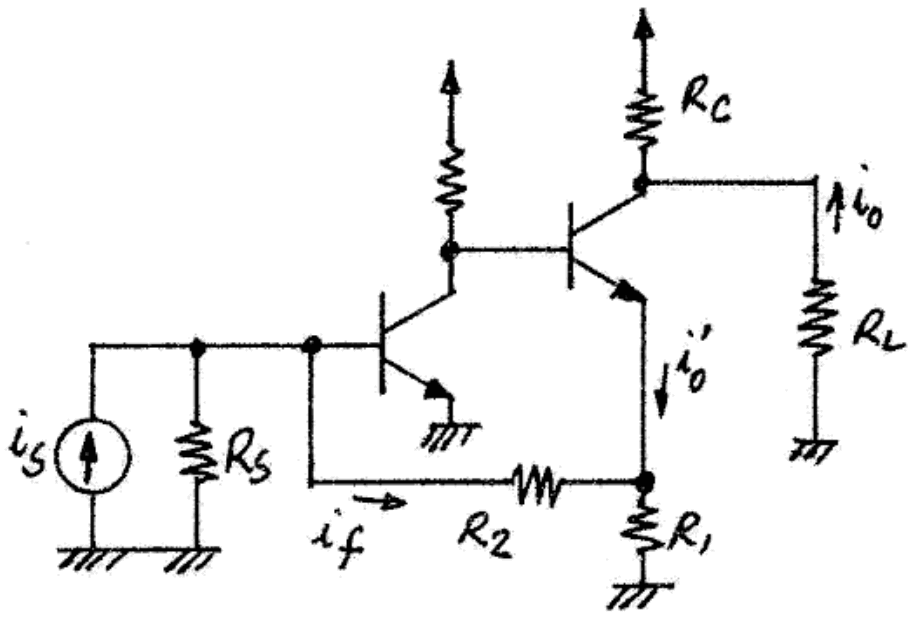
\includegraphics[width=0.6\linewidth]{_fig/retro_m-lazo_c-nodo_c.png}
	\caption{Muestreo de Lazo - Comparación de Nodo}
	\label{fig:retro_m-lazo_c-nodo_c}
\end{figure}

\subsection{Muestreo de Nodo - Comparación de Nodo} %p142

En la Figura \ref{fig:retro_m-nodo_c-nodo_a} se muestra el diagrama de bloques de este tipo de retroalimentación, donde las señales de interés son la tensión de salida y la corriente de entrada. La red $\beta$ de retroalimentación devuelve una corriente $i_f$ a la entrada, que es una muestra de la tensión de salida $v_0$. Por lo tanto, $\beta = i_f / v_0$, tiene unidades de conductancia. En cambio, el bloque $A$ representa una relación de tensión de salida en función de la corriente de entrada; $A_R = v_0 / i_s$, es decir, tiene unidades de resistencia.

\begin{figure}[h]
	\centering
	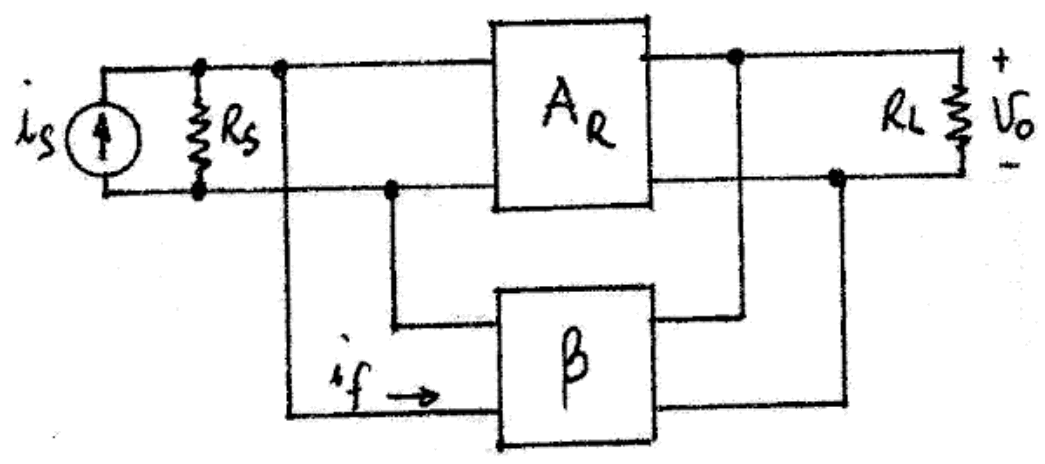
\includegraphics[width=0.6\linewidth]{_fig/retro_m-nodo_c-nodo_a.png}
	\caption{Muestreo de Nodo - Comparación de Nodo}
	\label{fig:retro_m-nodo_c-nodo_a}
\end{figure}

En la Figura \ref{fig:retro_m-nodo_c-nodo_b} se representa de nuevo este tipo de retroalimentación, pero ahora referenciando los cuadripolos a tierra. Además, ahora se ha indicado dentro del bloque de $\beta$ la configuración típica, que en este caso consiste simplemente de una resistencia.

\begin{figure}[h]
	\centering
	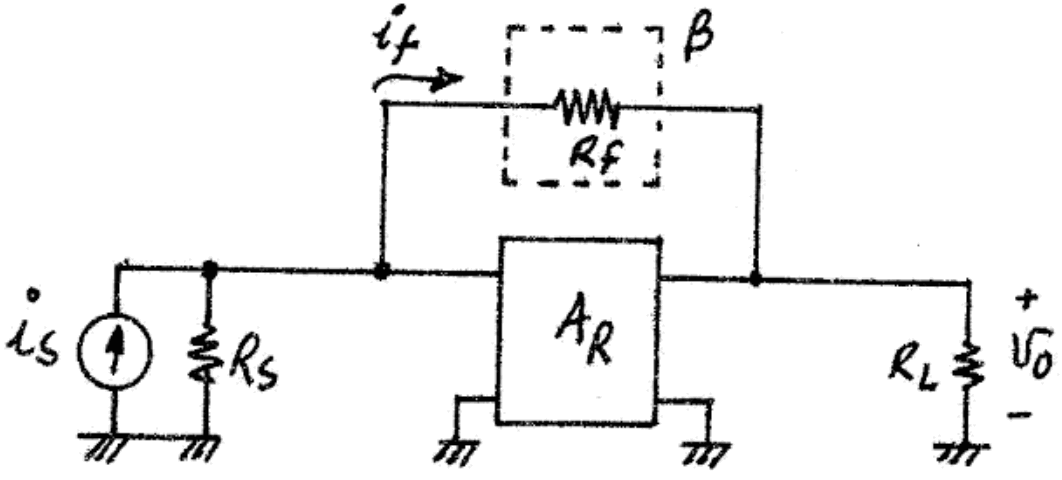
\includegraphics[width=0.6\linewidth]{_fig/retro_m-nodo_c-nodo.b.png}
	\caption{Muestreo de Nodo - Comparación de Nodo}
	\label{fig:retro_m-nodo_c-nodo_b}
\end{figure}

Además, en la Figura \ref{fig:retro_m-nodo_c-nodo_c} se muestran dos ejemplos de circuitos con este tipo de retroalimentación. Uno de ellos es la conocida configuración de ganancia negativa con el amplificador operacional.

\begin{figure}[h]
	\centering
	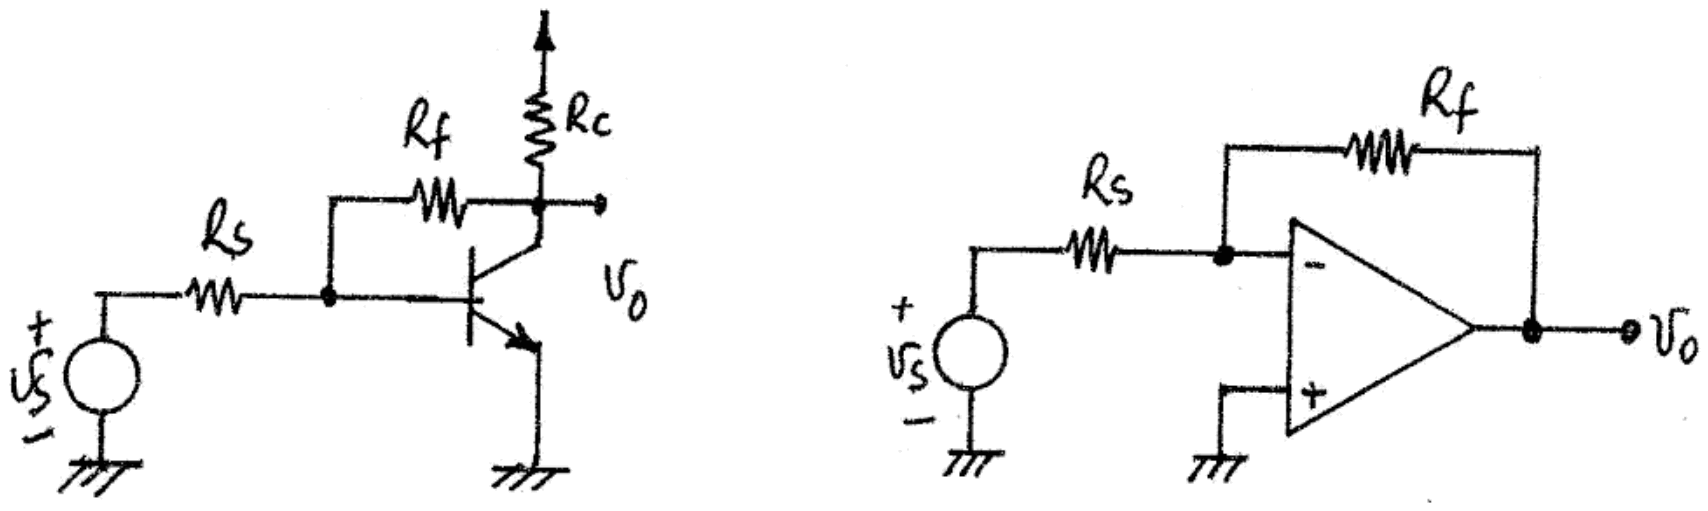
\includegraphics[width=0.6\linewidth]{_fig/retro_m-nodo_c-nodo_c.png}
	\caption{Muestreo de Nodo - Comparación de Nodo}
	\label{fig:retro_m-nodo_c-nodo_c}
\end{figure}

\subsection{Muestreo de Lazo - Comparación de Lazo} %p143

En la Figura \ref{fig:retro_m-lazo_c-lazo_a} se muestra el diagrama de bloques de este tipo de retroalimentación, donde las señales de interés son la corriente de salida y la tensión de entrada. La red $\beta$ de retroalimentación genera una tensión $v_f$ a la entrada, que es una muestra de la corriente de salida $i_o$; por lo tanto, $\beta = v_f / i_0$, tiene unidades de resistencia. En cambio, el bloque $A$ representa una relación de corriente de salida en función de la tensión de entrada, $A_G = i_o / v_s$, es decir, tiene unidades de conductancia.

\begin{figure}[h]
	\centering
	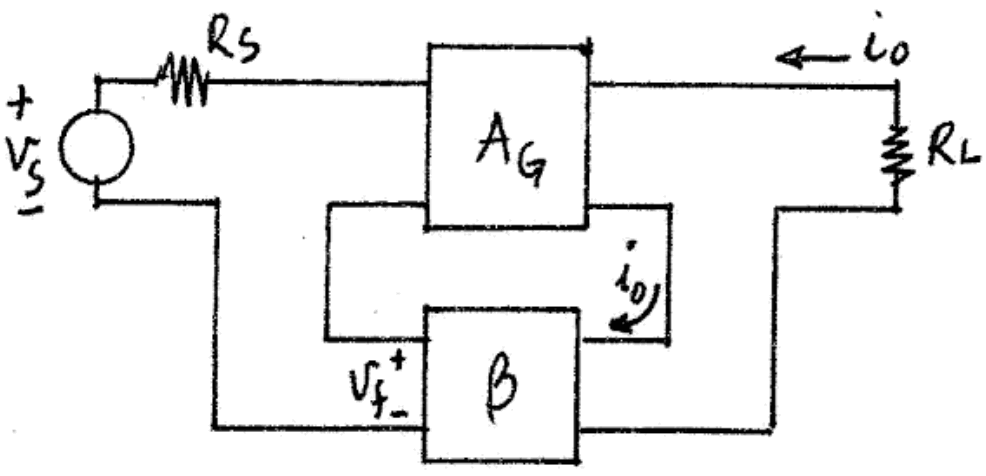
\includegraphics[width=0.8\linewidth]{_fig/retro_m-lazo_c-lazo_a.png}
	\caption{Muestreo de Lazo - Comparación de Lazo}
	\label{fig:retro_m-lazo_c-lazo_a}
\end{figure}

En la Figura \ref{fig:retro_m-lazo_c-lazo_b} se representa de nuevo este tipo de retroalimentación, pero ahora referenciando los cuadripolos a tierra. Además, ahora se ha indicado dentro del bloque de $\beta$ la configuración típica, que en este caso consiste simplemente en una resistencia.

\begin{figure}[h]
	\centering
	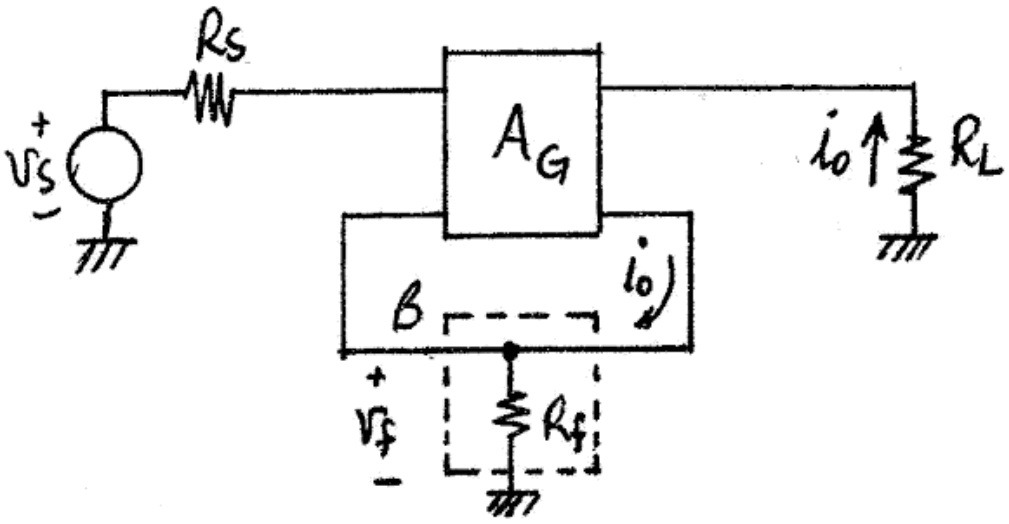
\includegraphics[width=0.8\linewidth]{_fig/retro_m-lazo_c-lazo_b.png}
	\caption{Muestreo de Lazo - Comparación de Lazo}
	\label{fig:retro_m-lazo_c-lazo_b}
\end{figure}

En la Figura \ref{fig:retro_m-lazo_c-lazo_c} se muestra un ejemplo de circuitos con este tipo de retroalimentación. Es la conocida configuración emisor común con $R_E$.

\begin{figure}[h]
	\centering
	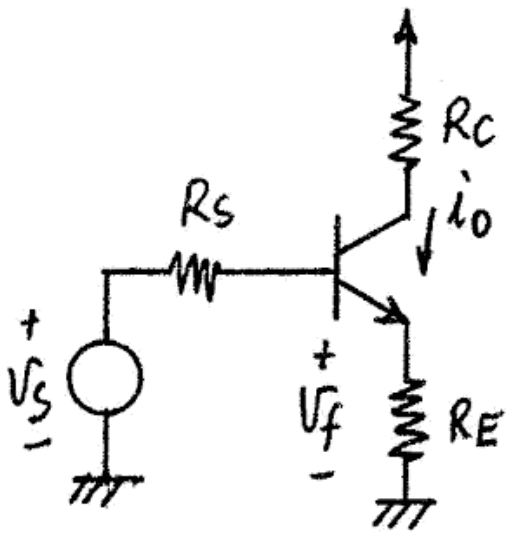
\includegraphics[width=0.6\linewidth]{_fig/retro_m-lazo_c-lazo_c.png}
	\caption{Muestreo de Lazo - Comparación de Lazo}
	\label{fig:retro_m-lazo_c-lazo_c}
\end{figure}

\section{Interpretación de Circuitos Como Lazo Cerrado con Retroalimentación} %p145

A continuación, presentaremos una metodología de análisis especial para circuitos con retroalimentación. Nos determinará condiciones necesarias que deben cumplirse, que permitirá hallar $A$ y $\beta$ por separado.

\subsection{Muestreo de Nodo - Comparación de Nodo} %p145

En la Figura \ref{fig:retro_m-nodo_c-nodo} se muestra un esquema idealizado de la retroalimentación Muestreo de Nodo - Comparación de Nodo. La resistencia de la fuente se ha incorporado a la $R_i$ del amplificador, y así mismo la $R_L$ de carga se ha incorporado con la $R_o$ de salida del amplificador (comparar con la Figura \ref{fig:retro_m-nodo_c-nodo_a}). En el diagrama tenemos el cuadrito perteneciente al amplificador sin retroalimentación $A$, con su resistencia de entrada sin retroalimentación, $R_i$, y su resistencia de salida sin retroalimentación, $R_o$. También se muestra un cuadrito de la retroalimentación $\beta$; tenemos la fuente de entrada $I_s$, la corriente retroalimentada $I_f$, la diferencia $I_i$, y el voltaje de salida $V_o$. Muy parecido al diagrama ideal.

\begin{figure}[h]
	\centering
	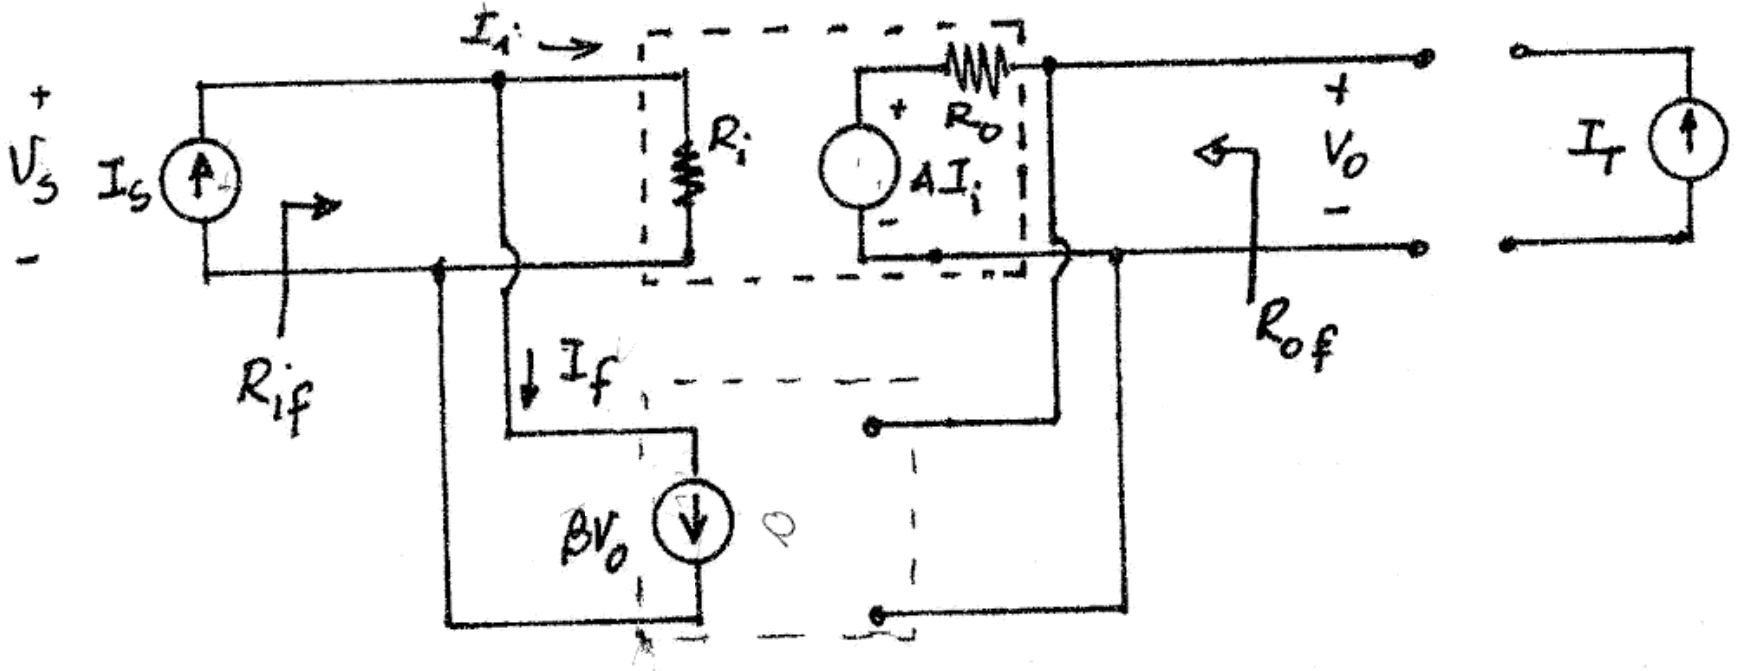
\includegraphics[width=0.9\linewidth]{_fig/retro_m-nodo_c-nodo.png}
	\caption{Muestreo de Nodo - Comparación de Nodo}
	\label{fig:retro_m-nodo_c-nodo}
\end{figure}

La ganancia con retroalimentación, $A_f$, es la relación entre el voltaje de salida y la corriente de entrada: $A_f = V_o / I_s$. Se tiene: \( V_o = A I_i = A (I_s - I_f) = A (I_s - \beta V_o) \) o:

\begin{equation}
	A_f = \frac{V_o}{I_s} = \frac{A}{1 + A\beta}
	\label{equ:retro_ganancia}
\end{equation}

Ésta es la relación clásica de retroalimentación.

La resistencia de entrada con retroalimentación, $R_{if}$, es la resistencia que se ve desde la fuente $I_s$. Se tiene:

\[
R_{if} = \frac{V_s}{I_s} = I_i \frac{R_i}{I_s} = \frac{(I_s - I_f) R_i}{I_s}
\]

\[
R_{if} = \frac{(I_s - \beta V_o) R_i}{I_s} = \frac{(I_s - \beta A I_s)}{(1 + A \beta)} \frac{R_i}{I_s}
\]

\begin{equation}
	R_{if} = \frac{R_i}{1 + A \beta}
	\label{equ:retro_rif}
\end{equation}

Entonces, con comparación de nudo, la resistencia de entrada con retroalimentación es igual a la resistencia de entrada del amplificador sin retroalimentación dividida por el factor $(1 + A \beta)$. Ver por ejemplo la Tabla \ref{tab:retro_comparativo}.

La resistencia de salida con retroalimentación es la resistencia vista desde los terminales de salida. Si inyectamos una fuente de corriente entre los bornes de salida y apagamos la fuente \( I_s \) de entrada, se obtienen los siguientes resultados:

\( V_o = I_T R_o + A I_i\), pero  \(I_i = -I_f = -\beta V_o \)

Entonces: \( V_o (1 + A \beta) = I_T R_o \) ó

\begin{equation}
	R_{of} = \frac{V_o}{I_T} = \frac{R_o}{1 + A \beta}
	\label{equ:retro_rof}
\end{equation}

Con muestreo de nudo, la resistencia de salida con retroalimentación es igual a la resistencia de salida del amplificador sin retroalimentación dividida por el factor \( (1 + A \beta) \). Nuevamente comparar con la Tabla \ref{tab:retro_comparativo}.

El esquema de la Figura \ref{fig:retro_m-nodo_c-nodo} se reduce al esquema de la Figura \ref{fig:retro_m-nodo_c-nodo_equi-reducido} con las equivalencias encontradas.

\begin{figure}[h]
	\centering
	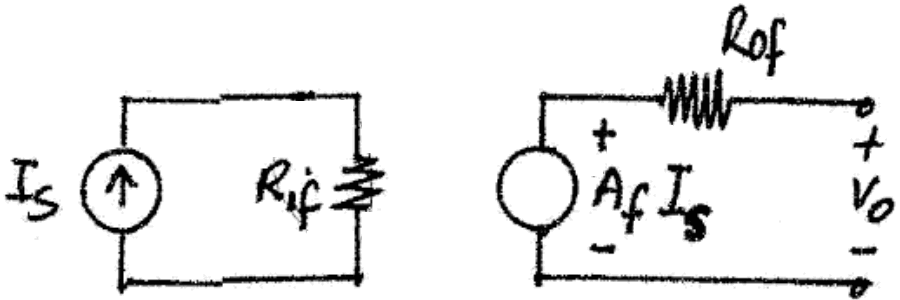
\includegraphics[width=0.7\linewidth]{_fig/retro_m-nodo_c-nodo_equi-reducido.png}
	\caption{Equivalente reducido de diagrama anterior.}
	\label{fig:retro_m-nodo_c-nodo_equi-reducido}
\end{figure}

Ahora lo que queremos es adaptar un circuito real, como el indicado en la Figura 3.40, a este esquema idealizado, para poder aplicar los resultados de las ecuaciones \ref{equ:retro_ganancia}, \ref{equ:retro_rif} y \ref{equ:retro_rof}.

Se reemplazan los bloques funcionales \( A \) y \( \beta \) por el cuadripolo apropiado según el tipo de retroalimentación. Con comparación de nodo, deberíamos escoger el cuadripolo de modo que la fuente y los elementos de entrada del cuadripolo se unan en un par de nodos comunes. De igual forma, con muestreo de nodo, queremos un cuadripolo con un par de nodos comunes a la salida. 

El cuadripolo \( y \), basado en las admitancias de cortocircuito, \( y_i \), \( y_o \), \( y_r \), cumple con estas condiciones. Queda la Figura \ref{fig:retro_m-nodo_c-nodo_cuadripolo}.

\begin{figure}[h]
	\centering
	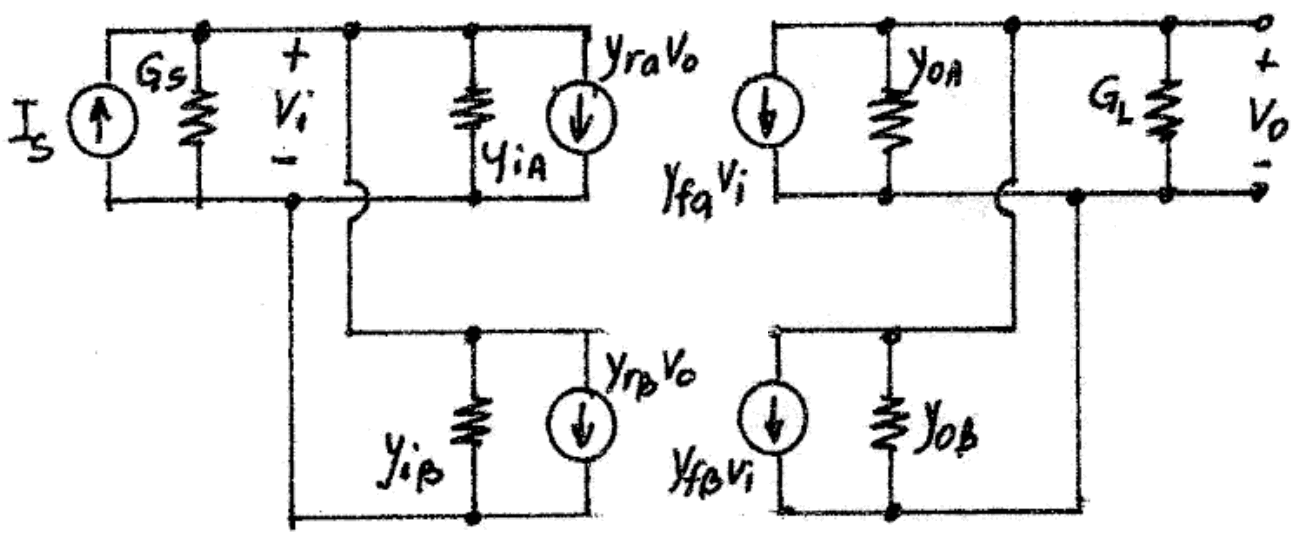
\includegraphics[width=0.9\linewidth]{_fig/retro_m-nodo_c-nodo_cuadripolo.png}
	\caption{Cuadripolo \( y \) aplicado a \( A \) y \( \beta \).}
	\label{fig:retro_m-nodo_c-nodo_cuadripolo}
\end{figure}

Se hace recordar que el cuadripolo \( y \) utiliza las tensiones de entrada y de salida como variables independientes, y las corrientes de entrada y salida como variables dependientes.

\begin{figure}[h]
	\centering
	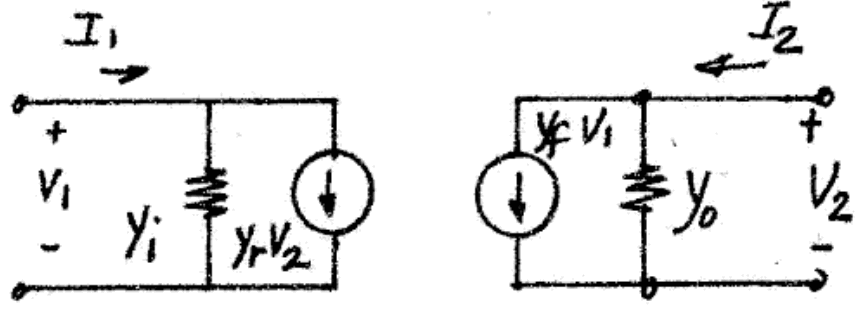
\includegraphics[width=0.9\linewidth]{_fig/retro_m-nodo_c-nodo_cuadripolo-y.png}
	\caption{Cuadripolo \( y \)}
	\label{fig:retro_m-nodo_c-nodo_cuadripolo-y}
\end{figure}			

Según se desprende de la Figura \ref{fig:retro_m-nodo_c-nodo_cuadripolo-y}, se obtiene:

\begin{equation}
	I_1 = y_{i} V_1 + y_{r} V_2
\end{equation}

\begin{equation}
	I_2 = y_{f} V_1 + y_{o} V_2
\end{equation}

donde:

\( y_{i} = \frac{I_{1}}{V_{1}} \) con la salida en cortocircuito, es la admitancia de entrada.

\( y_{r} = \frac{I_{1}}{V_{2}} \) con la entrada en cortocircuito, es la transadmitancia reversa.

\( y_{f} = \frac{I_{2}}{V_{1}} \) con la salida en cortocircuito, es la transadmitancia directa.

\( y_{o} = \frac{I_{2}}{V_{2}} \) con la salida en cortocircuito, es la admitancia de salida.

Volviendo a la Figura \ref{fig:retro_m-nodo_c-nodo_cuadripolo}, se obtiene:

\begin{equation}
	I_{s} = (G_s + Y_{1A} + Y_{1B}) V_{1} + (Y_{rA} + Y_{r \beta}) V_o
\end{equation}

\begin{equation}
	0 = (Y_{fA} + Y_{fB}) V_{1} + (G_{L} + Y_{oA} + Y_{o \beta}) V_o
\end{equation}

Dado que:

\begin{equation}
	Y_{i} = G_{s} + Y_{1A} + Y_{1B}
\end{equation}

\begin{equation}
	Y_{o} = G_{L} + Y_{oA} + Y_{oB}
\end{equation}

Entonces:

\begin{equation}
	\frac{V_o}{I_s} = \frac{-(Y_{fA} + Y_{fB})}{Y_i Y_o - (Y_{rA} + Y_{rB})(Y_{fA} + Y_{fB})}
\end{equation}

Para llevar esta expresión a la forma clásica de la ganancia con retroalimentación, se puede organizar de la siguiente forma:

\begin{equation}
	\frac{V_o}{I_s} = \frac{-(Y_{fA} + Y_{fB}) / Y_i Y_o}{1 - (Y_{rA} + Y_{rB}) / Y_i}
\end{equation}

de donde:

\begin{equation} \label{equ:retro_m-nodo_c-nodo_orig-A}
	A = \frac{-(Y_{fA} + Y_{fB})}{Y_i Y_o}
\end{equation}

y:

\begin{equation} \label{equ:retro_m-nodo_c-nodo_orig-B}
	\beta = Y_{rA} + Y_{rB}
\end{equation}

Para poder interpretar fácilmente estas expresiones, se hacen las siguientes suposiciones, que posteriormente se convertirán en condiciones necesarias para poder aplicar nuestro método:

\textbf{a)} el amplificador da más ganancia en sentido directo que la red de retroalimentación, es decir:

\begin{equation} \label{equ:retro_m-nodo_c-nodo_admitancia-yfA}
	|Y_{fA}| >> |Y_{fB}|
\end{equation}

\textbf{b)} la señal retroalimentada a la entrada de la salida se debe más a la red de retroalimentación que al amplificador, es decir:

\begin{equation} \label{equ:retro_m-nodo_c-nodo_admitancia-yfB}
	|Y_{rA}| << |Y_{rB}|
\end{equation}

\textbf{c)} la admitancia de salida no afecta mucho la admitancia de entrada, es decir:

\begin{equation} \label{equ:retro_m-nodo_c-nodo_admitancias}
	|Y_{fA} Y_{rA}| << |Y_i Y_o|
\end{equation}

Entonces la expresión \ref{equ:retro_m-nodo_c-nodo_orig-A} se convierte en la siguiente:

\[ A = -Y_{fA} / Y_i Y_o \]

\begin{equation} \label{equ:retro_m-nodo_c-nodo_A}
	A = -Y_{fA} / (G_s + Y_{iA} + Y_{iB}) (G_L + Y_{oA} + Y_{oB})
\end{equation}

donde se destaca la presencia de componentes de la red $\beta$. Y la expresión \ref{equ:retro_m-nodo_c-nodo_orig-B} se convierte en:

\begin{equation} \label{equ:retro_m-nodo_c-nodo_B}
	\beta \cong Y_{rB}
\end{equation}

que depende solo de la red $\beta$.

\begin{figure}[h]
	\centering
	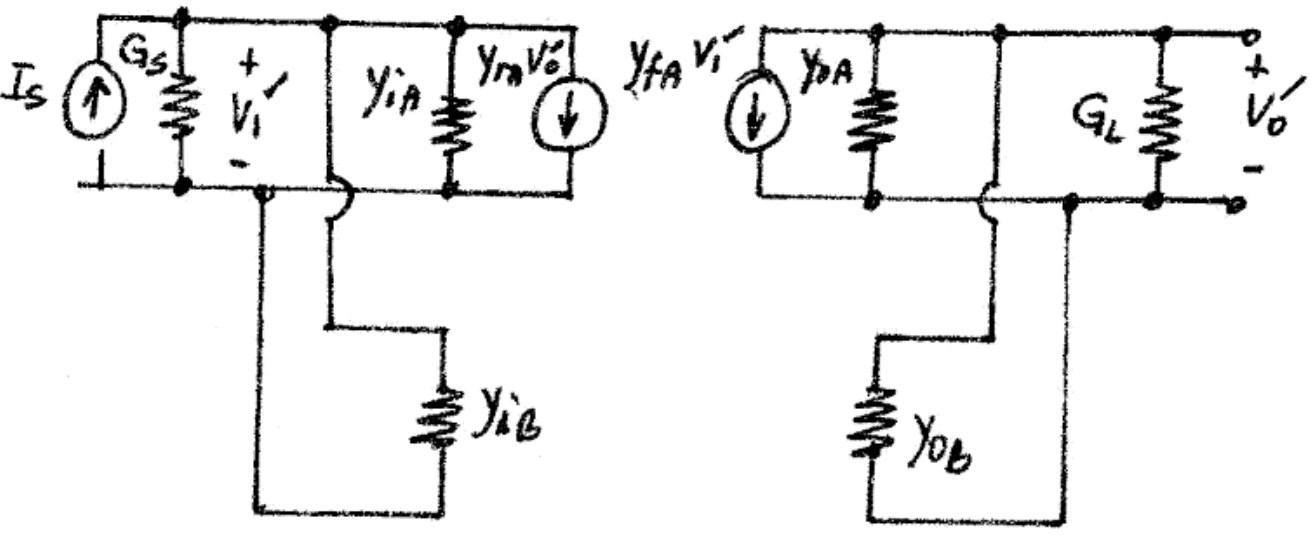
\includegraphics[width=0.9\linewidth]{_fig/retro_m-nodo_c-nodo_hallar-a.png}
	\caption{Circuito para hallar \( A = \frac{V_o}{I_s} \)}
	\label{fig:retro_m-nodo_c-nodo_hallar-a}
\end{figure}			

La expresión \ref{equ:retro_m-nodo_c-nodo_A} para A tiene una interpretación circuital muy interesante que se indica en la Figura \ref{fig:retro_m-nodo_c-nodo_hallar-a}. De este circuito se consigue:

\begin{equation} \label{equ:retro_m-nodo_c-nodo_solve-A}
	A = V_o^{\prime} / I_s = -Y_{fA} / (Y_i Y_o - Y_{fA} Y_{rA})
\end{equation}

\begin{figure}[h]
	\centering
	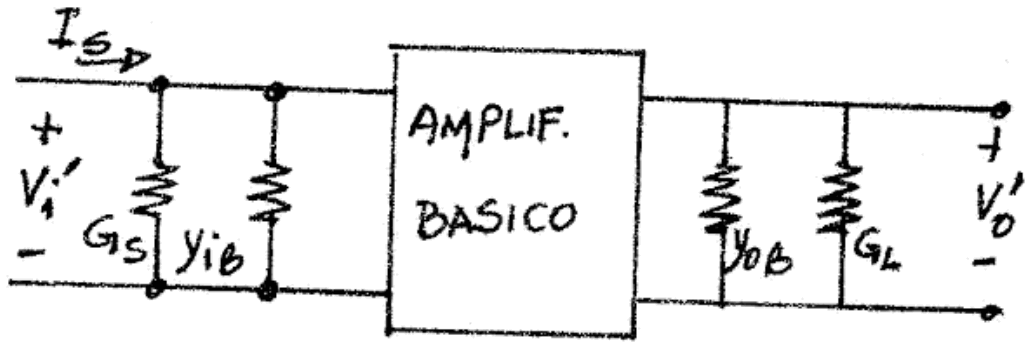
\includegraphics[width=0.9\linewidth]{_fig/retro_m-nodo_c-nodo_solve-hallar-a.png}
	\caption{Circuito para hallar \( A \) compacto}
	\label{fig:retro_m-nodo_c-nodo_solve-a}
\end{figure}

pero si es aplicable la desigualdad \ref{equ:retro_m-nodo_c-nodo_admitancias} entonces la ecuación \ref{equ:retro_m-nodo_c-nodo_solve-A} se reduce a la ecuación \ref{equ:retro_m-nodo_c-nodo_A}. ¿Y cual es el circuito de la Figura \ref{fig:retro_m-nodo_c-nodo_hallar-a}? Es el circuito original con la retroalimentación eliminada, pero con el efecto de carga de la red de retroalimentación incluido, tal como se aprecia más claramente en la Figura \ref{fig:retro_m-nodo_c-nodo_solve-a}. Es decir, nos queda la fuente de entrada con su resistencia, la salida con su resistencia de carga, el amplificador completo, a la entrada se anexa $Y_{iB}$, la admitancia de entrada de la red de retroalimentación con la salida en cortocircuito, y a la salida se anexa \( Y_{oB} \), la admitancia de salida de la red de retroalimentación con la entrada en cortocircuito. Al finalizar esta sección resolveremos ejemplos donde se aplicará este análisis.

En cuanto a la retroalimentación, con la aplicación de las desigualdades, nos queda:

\begin{equation}
	\beta = Y_{rB}
\end{equation}

\begin{figure}[h]
	\centering
	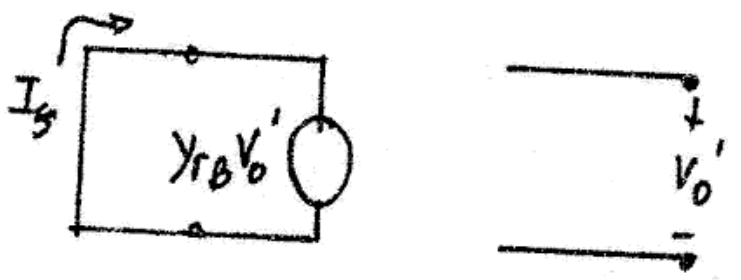
\includegraphics[width=0.9\linewidth]{_fig/retro_m-nodo_c-nodo_admitancia-reversa.png}
	\caption{Admitancia reversa}
	\label{fig:retro_m-nodo_c-nodo_admitancia-reversa}
\end{figure}

la admitancia reversa de la red de retroalimentación, que se encuentra como la relación de la corriente de retroalimentación a la tensión de salida con la entrada en cortocircuito, como se indica en la Figura \ref{fig:retro_m-nodo_c-nodo_admitancia-reversa}.

Antes de seguir con los ejemplos, vamos a demostrar el efecto de la retroalimentación sobre las admitancias de entrada y salida para el caso de Muestreo de Nodo - Comparación de Nodo.

\begin{figure}[h]
	\centering
	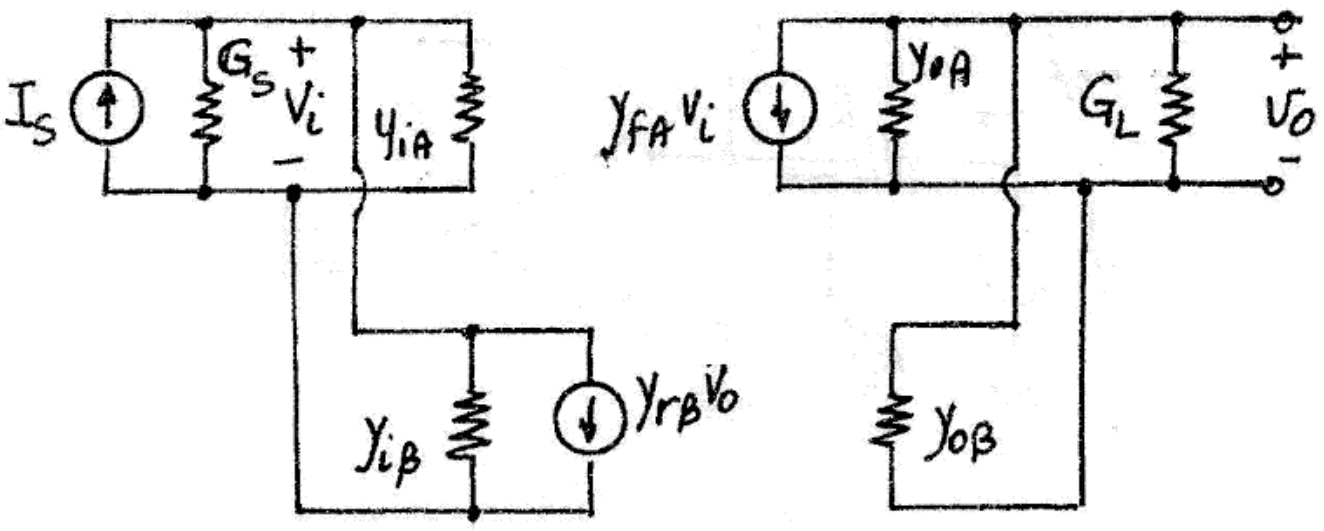
\includegraphics[width=0.9\linewidth]{_fig/retro_m-nodo_c-nodo_admitancia-entrada.png}
	\caption{Admitancia de entrada}
	\label{fig:retro_m-nodo_c-nodo_admitancia-entrada}
\end{figure}

En la Figura \ref{fig:retro_m-nodo_c-nodo_admitancia-entrada}, se busca la admitancia de entrada con el modelo general, donde se ignora \( Y_{fB} A \) y \( Y_{rA} \) por considerarlos despreciables, según la discusión anterior. Nos queda:

\begin{equation}
	I_s = V_i (G_s + Y_{iA} + Y_{iB}) + Y_{rB} V_o
\end{equation}

e,

\begin{equation}
	( Y_{oA}  + G_L + Y_{oB} ) = -Y_{fA} V_i
\end{equation}

ó, $ V_o = -(\frac{Y_{fA}}{Y_o} V_i $, de donde $ I_s = V_i (Y_i - \frac{Y_{fA}Y_{rB}}{Y_o} ) = V_i ( Y_i ( 1 - \frac{Y_{fA}}{Y_i Y_{o}} ) Y_{rB}) $ ó

\begin{equation}
	\frac{I_s}{V_i} = Y_i (1 + A\beta).
\end{equation}

es decir, la admitancia de entrada aumenta por el factor \( 1 + A\beta \); la resistencia de entrada se reduce por \( 1 + A\beta \).

En la Figura \ref{fig:retro_m-nodo_c-nodo_sch-ext}, se muestra el circuito a analizar para hallar la admitancia en los nodos de salida. Entonces:

\begin{equation}
	I_T = V_o (G_L + y_{oA} + y_{oB}) + y_{fA} V_i 
\end{equation}

\begin{equation}
	V_i (G_s + y_{iA} + y_{iB}) = -y_{fB} V_o
\end{equation}

o,

\[
V_i = -\left( \frac{y_{fB}}{G_s + y_{iA} + y_{iB}} \right) V_o
\]

Luego,

\begin{equation}
	I_T = V_o \left( G_L + y_{oA} + y_{oB} - y_{fA} \frac{y_{fB}}{G_s + y_{iA} + y_{iB}} \right)
\end{equation}

o bien,

\begin{equation}
	\frac{I_T}{V_o} = G_L + y_{oA} + y_{oB} - \frac{y_{fA} y_{fB}}{G_s + y_{iA} + y_{iB}}
\end{equation}

es decir, la admitancia de salida aumenta por el factor $1 + AB$.

\begin{figure}[h]
	\centering
	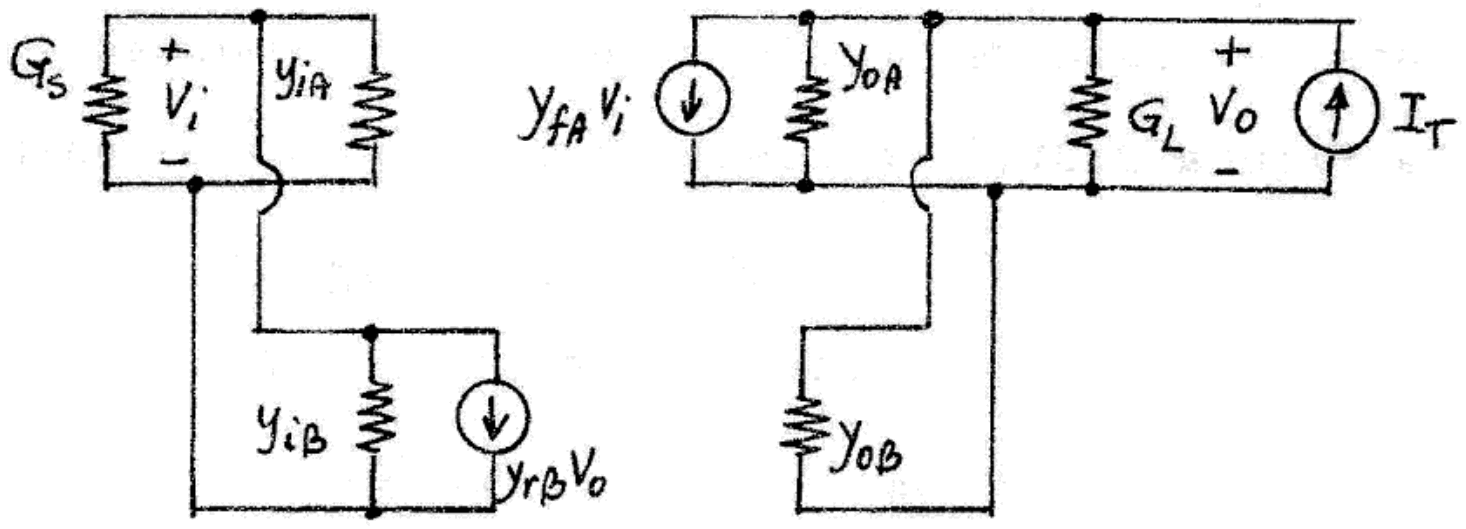
\includegraphics[width=0.8\linewidth]{_fig/retro_m-nodo_c-nodo_sch-ext.png}
	\caption{Circuito equivalente para hallar admitancia}
	\label{fig:retro_m-nodo_c-nodo_sch-ext}
\end{figure}

Ahora, vamos a resolver un par de ejemplos para demostrar la aplicación de la teoría que se acaba de describir.

\subsubsection{Ejemplo A} %p152

En la Figura \ref{fig:retro_m-nodo_c-nodo_ejm1a} se muestra un amplificador con retroalimentación.

\begin{figure}[h]
	\centering
	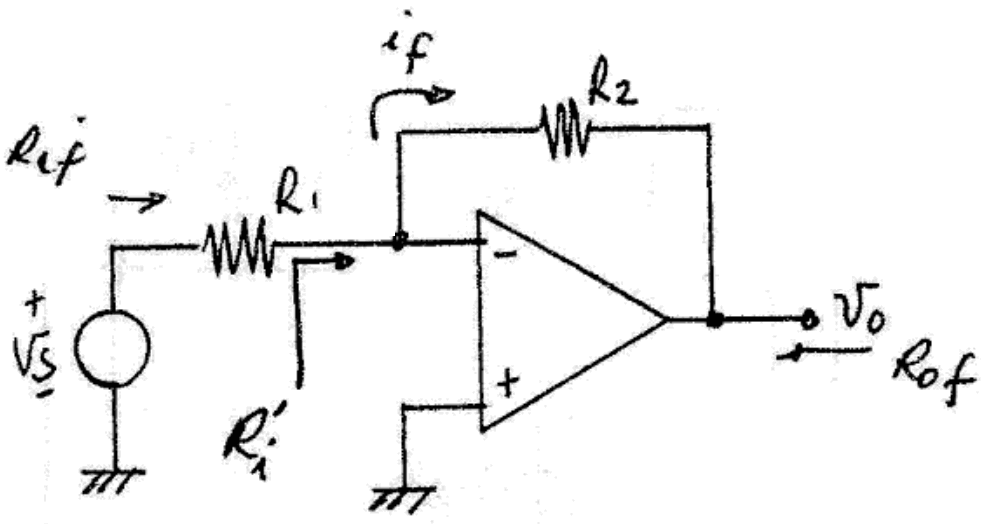
\includegraphics[width=0.6\linewidth]{_fig/retro_m-nodo_c-nodo_ejm1a.png}
	\caption{Ejemplo: Circuito amplificador con retroalimentación}
	\label{fig:retro_m-nodo_c-nodo_ejm1a}
\end{figure}

Lo \textbf{Primero} que hace falta es identificar el tipo de retroalimentación: la retroalimentación se crea por medio de la rama \( R_2 \). Esta rama llega al mismo nodo de entrada, y por lo tanto es comparación de nodo. En la salida, se toma la señal de retroalimentación en el nodo de salida, por lo tanto es muestreo de nodo, es decir, se muestra la tensión de salida.

Lo \textbf{Segundo} es hallar el punto de operación. Con los operacionales este paso no es necesario ya que la polarización consiste sencillamente en conectar las fuentes de DC.

\textbf{Tercero}, se crea el amplificador \( A \) en lazo abierto. Se elimina la red de retroalimentación para dejar el amplificador sin retroalimentación, al cual se anexa a la entrada y a la salida el efecto de carga de la red de retroalimentación siguiendo los pasos previamente establecidos. El resultado se muestra en la Figura \ref{fig:retro_m-nodo_c-nodo_ejm1b}.

\begin{figure}[h]
	\centering
	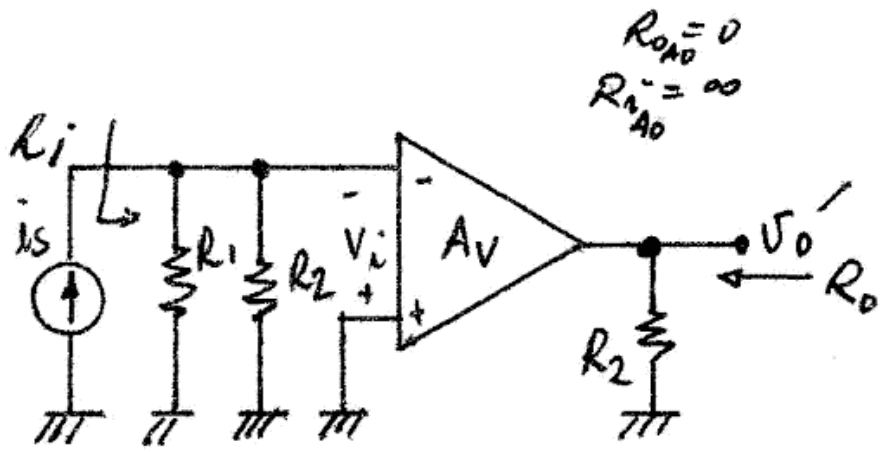
\includegraphics[width=0.6\linewidth]{_fig/retro_m-nodo_c-nodo_ejm1b.png}
	\caption{Circuito amplificador con retroalimentación}
	\label{fig:retro_m-nodo_c-nodo_ejm1b}
\end{figure}

Nuevamente hemos convertido la fuente de entrada, junto con su resistencia, en el equivalente de Norton por considerarse de una retroalimentación tipo comparación de nodo. De aquí se obtiene:

\[
A = \frac{v_o'}{i_s} = -A_V (R_1 || R_2)
\]

\[
R_i = R_1 || R_2
\]

\[
R_o = 0
\]

y la respuesta de frecuencia sin retroalimentación.

\textbf{Cuarto}, se encuentra \( \beta \). La red de retroalimentación está formada por \( R_2 \).  \( \beta \) viene dada por \( \frac{i_f}{v_o} \) con la entrada en cortocircuito, o \( \frac{i_f}{v_o} = \frac{-1}{R_2} \)

Próximamente, dado los valores sin retroalimentación, y \( \beta \), se determinan las características del circuito con retroalimentación. Tenemos:

\[
D = 1 + A\beta = 1 + A_V R_1 / (R_1 + R_2)
\]

\[
A_f = A / D = -A_V (R_1 || R_2) / \left(1 + A_V R_1 / (R_1 + R_2)\right)
\]

\[
R_{if} = R_i / D = R_1 || R_2 / \left(1 + A_V R_1 / (R_1 + R_2)\right)
\]

\[
R_{of} = R_o / D = 0
\]

\[
\frac{v_o}{v_s} = v_o (i_s R) = \frac{A_f}{R_i} = -\frac{R_2}{R_1} \frac{1}{1 + (1 + R_2 / R_1) / A_V}
\]

Finalmente encontramos de nuevo la resistencia de entrada por medio de esta técnica de retroalimentación que se encontró previamente "a pie". Así:

\[
R_i' = \frac{1}{\left( \frac{1}{R_{if}} - \frac{1}{R_1} \right)} = \frac{R_2}{1 + A_V}
\]

\subsubsection{Ejemplo B} %p154

En la Figura \ref{fig:retro_m-nodo_c-nodo_ejm2a} se muestra un amplificador con retroalimentación.

\begin{figure}[h]
	\centering
	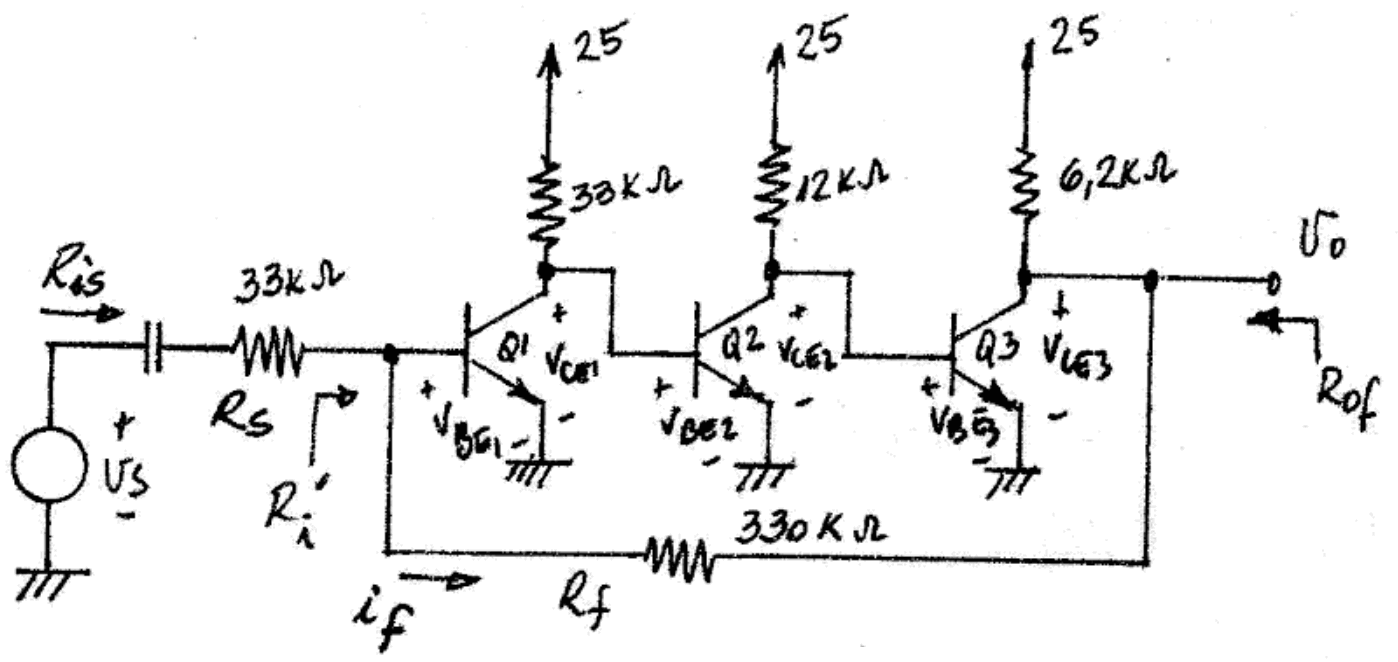
\includegraphics[width=0.8\linewidth]{_fig/retro_m-nodo_c-nodo_ejm2a.png}
	\caption{Ejemplo}
	\label{fig:retro_m-nodo_c-nodo_ejm2a}
\end{figure}

\textbf{Primero:} Identificación del tipo de retroalimentación: la retroalimentación se crea por medio de la rama \( R_f \). Esta rama llega al mismo nodo de entrada, y por lo tanto es comparación de nodo. En la salida, se toma la señal de retroalimentación en el nodo de salida, por lo tanto es muestreo de nodo, es decir se muestrea la tensión de salida.

\textbf{Segundo:} Hallar el punto de operación. En continua queda el circuito que se muestra en la Figura \ref{fig:retro_m-nodo_c-nodo_ejm2b}.

\begin{figure}[h]
	\centering
	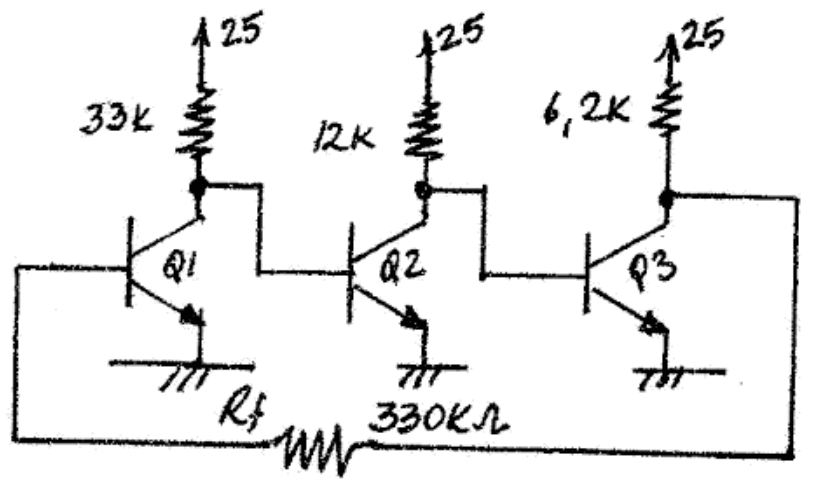
\includegraphics[width=0.7\linewidth]{_fig/retro_m-nodo_c-nodo_ejm2b.png}
	\caption{Circuito en dc de la Figura \ref{fig:retro_m-nodo_c-nodo_ejm2a}}
	\label{fig:retro_m-nodo_c-nodo_ejm2b}
\end{figure}

Primero se hace la observación que la misma tensión base-emisor es el voltaje colector-emisor de la etapa anterior, al menos en el acople del primer transistor con el segundo, y del segundo transistor con el tercero. Entonces

\[ V_{CE1} = V_{BE2} = 0.7V \]

\[ V_{CE2} = U_{BE3} = 0.7V \]

Ambos resultados nos garantizan \( V_{CE} > V_{CE(sat)} = 0.2V \) por lo que estamos fuera de la región de saturación. De aquí podemos calcular las corrientes de colector de los primeros dos transistores:

\[ I_{C1} \approx \frac{25 - 0.7}{33K} = 0.74 mA \]

\[ I_{C2} \approx \frac{25 - 0.7}{12K} = 2.02 mA \]

Para \( Q3 \) nos queda:

\[ 25 = I_{C3} \cdot 6.2K + I_{B1} \cdot 330K + 0.7 \]

De donde:

\[ I_{C3} = 3.5 mA \]

\[ V_{CE3} = 3.2 V \]

\textbf{Tercero:} Con estos valores de los puntos de operación se calculan los valores de los parámetros de los transistores:

\begin{tabular}{ccc}
	\( q_{m1} = 0.0285 \) & \( q_{m2} = 0.0777 \) & \( q_{m3} = 0.135 \) \\
	\( r_{\pi1} = 3513 \) & \( r_{\pi2} = 1287 \) & \( r_{\pi3} = 748 \) \\
\end{tabular}

\begin{figure}[h]
	\centering
	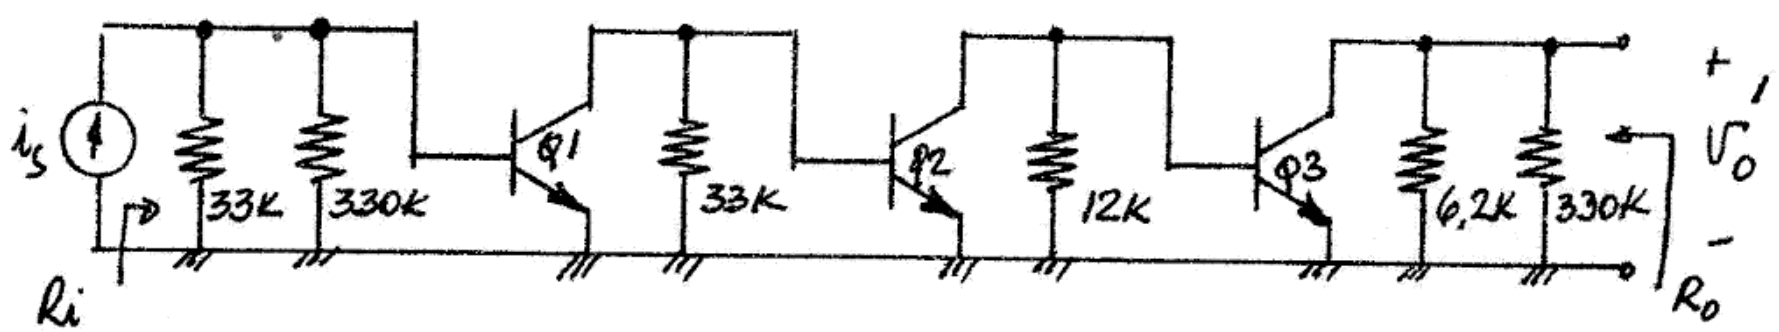
\includegraphics[width=0.8\linewidth]{_fig/retro_m-nodo_c-nodo_ejm2c.png}
	\caption{Circuito sin Retroalimentación, parte A}
	\label{fig:retro_m-nodo_c-nodo_ejm2c}
\end{figure}
\begin{figure}[h]
	\centering
	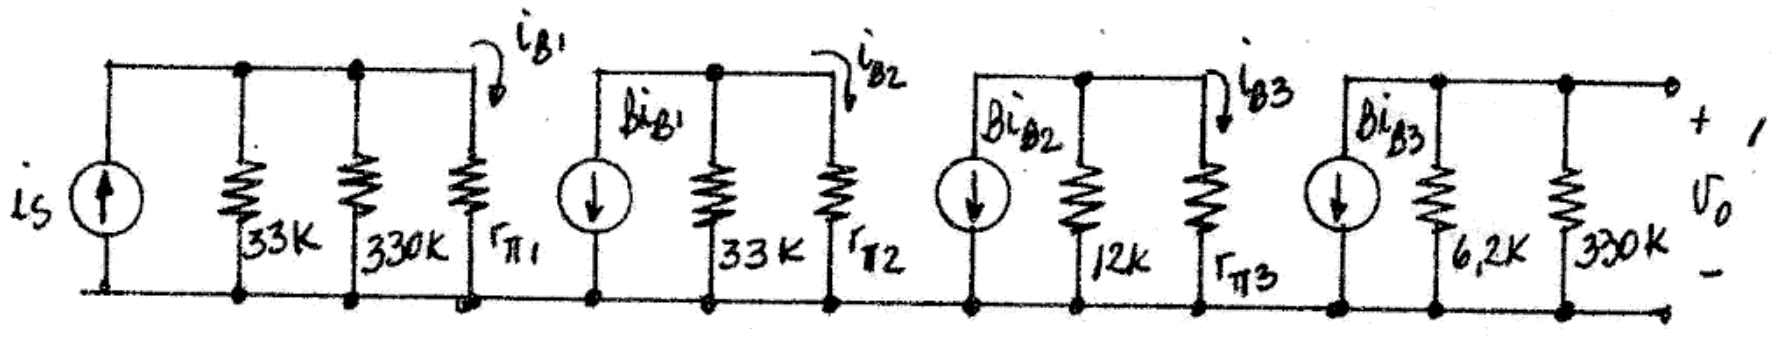
\includegraphics[width=0.8\linewidth]{_fig/retro_m-nodo_c-nodo_ejm2d.png}
	\caption{Circuito sin Retroalimentación, parte B}
	\label{fig:retro_m-nodo_c-nodo_ejm2d}
\end{figure}

Se elimina la red de retroalimentación para dejar el amplificador sin retroalimentación, al cual se anexa a la entrada y a la salida el efecto de carga de la red de retroalimentación. El resultado se muestra en la Figura \ref{fig:retro_m-nodo_c-nodo_ejm2c}, con su circuito equivalente a frecuencias medidas en la Figura \ref{fig:retro_m-nodo_c-nodo_ejm2d}.

Se hace notar que hemos convertido la fuente de entrada, junto con su resistencia, en el equivalente de Norton por considerarse de una retroalimentación tipo comparación de nodo. De aquí procedemos normalmente para obtener:

\[ A = \frac{i_o\prime\prime}{i_s} = -503 \]

\[ R_i = 1785 \]

\[ R_o = \infty \]

De querer la respuesta de frecuencia sin retroalimentación se volverían a colocar los condensadores, y se trabajaría con el modelo de alta frecuencia del transistor.

\textbf{Cuarto:} La red de retroalimentación está formada por $R_f$. $\beta$ viene dada por: $\frac{i_s}{v_o} = -\frac{1}{R_f}$

\textbf{Quinto:} Dados los valores sin retroalimentación, \( A \) y \( \beta \), se determinan las características del circuito con retroalimentación. Tenemos:

\[ D = 1 + A\beta = 14962 \]

\[ A_f = \frac{A}{D} = -329978 \Omega \]

\[ R_{if} = \frac{R_i}{D} = 0.21 \Omega	\]

\[ R_{of} = \frac{R_o}{D} = 0.41 \Omega	\]

\[ \frac{v_o}{v_s} = \frac{v_o}{(i_s R_s)} = \frac{A_f}{R} = -9.9993 \approx -10 \]

Finalmente, encontramos resistencias de entrada. Así:

\[ R_i' = \left( \frac{1}{R_{if}} - \frac{1}{R_s} \right)^{-1} = 0.21 \Omega \]

\[ R_{is} = R_s + R_i' \approx R_s = 33 k\Omega	\]

De esta forma, hemos analizado a fondo la metodología de retroalimentación aplicada al caso \textbf{Muestreo de Nodo - Comparación de Nodo}. A continuación, se tratan los otros casos de retroalimentación. El análisis es muy parecido, lo que permitirá acortar un poco su presentación.

\subsection{Muestreo de Lazo - Comparación de Lazo} %p157

\begin{figure}[h]
	\centering
	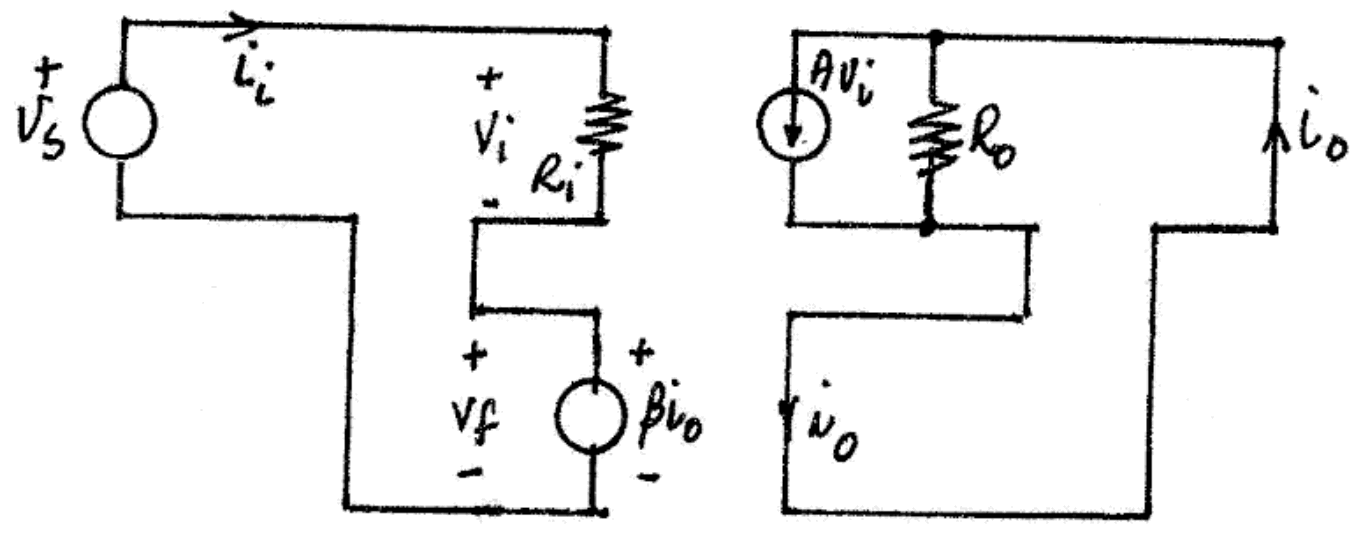
\includegraphics[width=0.8\linewidth]{_fig/retro_m-lazo_c-lazo.png}
	\caption{Muestreo de Lazo - Comparación de Lazo}
	\label{fig:retro_m-lazo_c-lazo}
\end{figure}

En la Figura \ref{fig:retro_m-lazo_c-lazo}, tenemos el diagrama idealizado de la retroalimentación tipo \textbf{Muestreo de Lazo - Comparación de Lazo}.

De la figura se obtienen las siguientes relaciones:

\textbf{Ganancia:}

\[ A_f = \frac{i_o}{v_s} \]

\[ i_o = A v_i \]

\[ v_i = v_s - v_f = v_s - \beta i_o \]

\[ i_o = A (v_s - \beta i_o) \]

\[ i_o (1 + A \beta) = A v_s \]

\[ A_f = \frac{i_o}{v_s} = \frac{A}{(1 + A \beta)} \]

\textbf{Resistencia de Entrada;}

\[ R_{if} = \frac{v_s}{i_i}	\]

\[ R_i = \frac{v_i}{i_i} \]

\[ v_s = i_i R_i + \beta i_o = i_I R_i + \frac{\beta A v_s}{1 + A \beta)} \]

\[ v_s \frac{1 - \beta A}{1 + A \beta} = i_i R_i \]

o

\[ R_{if} = \frac{v_s}{i_i} = R_i (1 + A \beta)	\]

Es decir, la resistencia del lazo de entrada aumenta por \( (1 + A \beta) \).

\textbf{Resistencia del Lazo de Salida:}

\begin{equation} \label{retro_m-lazo_c-lazo_rof}
	R_{of} = \frac{v_T}{I_T}
\end{equation}

\begin{figure}[h]
	\centering
	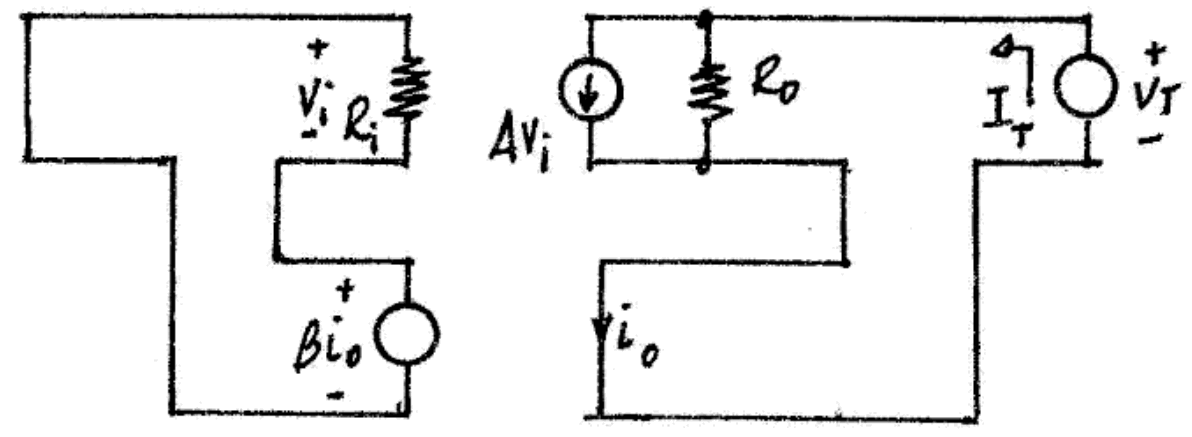
\includegraphics[width=0.8\linewidth]{_fig/retro_m-lazo_c-lazo_analisis-r.png}
	\caption{Muestreo de Lazo - Comparación de Lazo, análisis \( Rof \)}
	\label{fig:retro_m-lazo_c-lazo_analisis-r}
\end{figure}

Ecuacion \ref{retro_m-lazo_c-lazo_rof} según Figura \ref{fig:retro_m-lazo_c-lazo_analisis-r}

Donde:

\[ I_T = A v_i + \frac{v_T}{R_o} \]

\[ v_i = -\beta i_o = -\beta I_T \]

\[ I_T = -\beta A I_T + \frac{v_T}{R_o} \]

o:

\[ I_T (1 + A \beta) = \frac{v_T}{R_o} \]

y:

\[ R_{of} = \frac{v_T}{I_T} = Ro (1 + A \beta) \]

La resistencia del lazo de salida aumenta por \( (1 + A \beta) \). Cuando hablamos de la resistencia del lazo, eso implica abrir el lazo y determinar la resistencia desde el punto abierto, lo que normalmente conlleva a sumar las resistencia en el lazo.

En la figura \ref{fig:retro_m-lazo_c-lazo_a} se traza nuevamente el diagrama de bloques general de Muestreo de Lazo - Comparación de Lazo.

Se reemplaza los bloques funcionales de $A$ y $\beta$ por el cuadripolo apropiado según el tipo de retroalimentación. Con comparación de lazo deberíamos escoger el cuadripolo de modo que la fuente y los elementos de entrada del cuadripolo compartan un lazo común. De igual forma con muestreo de lazo queremos un lazo común a la salida. El cuadripolo $"z"$, basado en las impedancias de circuito abierto, $z_i$, $z_r$, $z_f$, $z_o$ cumple con éstas condiciones. Queda la figura \ref{fig:retro_m-lazo_c-lazo_modelo-cuadripolo-z}.

\begin{figure}[h]
	\centering
	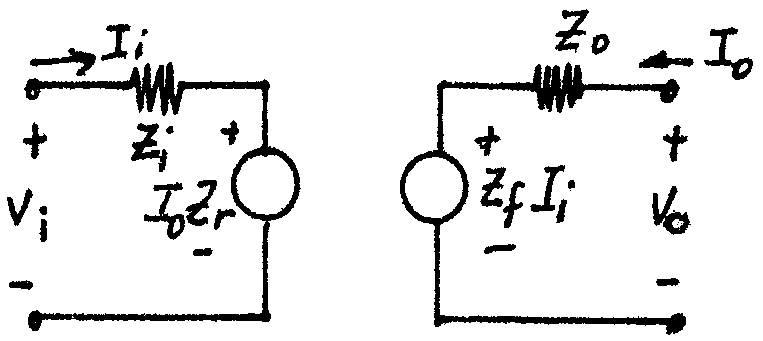
\includegraphics[width=0.6\linewidth]{_fig/retro_m-lazo_c-lazo_modelo-cuadripolo-z.png}
	\caption{Cuadripolo "z"}
	\label{fig:retro_m-lazo_c-lazo_modelo-cuadripolo-z}
\end{figure}

El cuadripolo \( Z \) utiliza las corrientes de entrada y de salida como variables independientes, y las tensiones de entrada y salida como variables dependientes. Se obtiene:

\begin{equation}
	Vi = I_i Z_i + I_o Z_r
\end{equation}			

\begin{equation}
	Vo = I_i Z_f + I_o Z_o
\end{equation}			

Nos queda el modelo de cuadripolos de Muestreo de Lazo - Comparación de Lazo en la Figura \ref{fig:retro_m-lazo_c-lazo_modelo-cuadripolo}.

\begin{figure}[h]
	\centering
	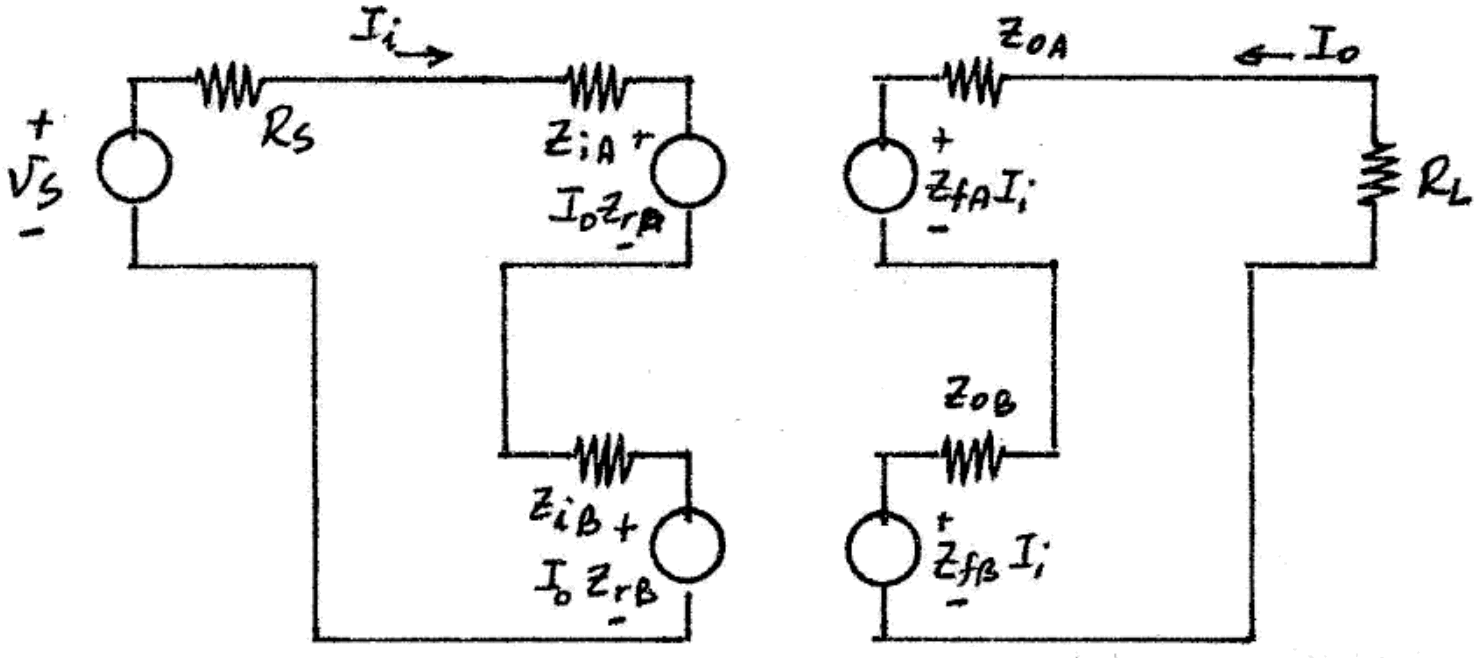
\includegraphics[width=0.8\linewidth]{_fig/retro_m-lazo_c-lazo_modelo-cuadripolo.png}
	\caption{Muestreo de Lazo - Comparación de Lazo}
	\label{fig:retro_m-lazo_c-lazo_modelo-cuadripolo}
\end{figure}

Procediendo como en el caso anterior, si se cumplen las siguientes condiciones: \( |Z_{fA}| \gg |Z_{fB}| \) , \( |Z_{oB}| \gg |Z_{oA}| \) , y \( |Z_{fA} Z_{rA}| \ll |Z_i Z_o| \) , entonces se puede aplicar la Metodología de Retroalimentación, y hallar \( A \) y \( \beta \) por separado.

El circuito de \( A \), el amplificador sin retroalimentación, se muestra en la Figura \ref{fig:retro_m-lazo_c-lazo_hallar-a}, donde se aprecia el anexo de \(Z_{i\beta}\) a la entrada y \(Z_{o\beta}\) a la salida. Se hace notar que \(Z_{i\beta}\) es la impedancia de entrada del circuito de retroalimentación con el lazo de salida abierto, mientras que \(Z_{o\beta}\) es la impedancia de salida del circuito de retroalimentación con el lazo de entrada abierto.

\begin{figure}[h]
	\centering
	\subfloat[Amplificador sin retroalimentación]
	{
		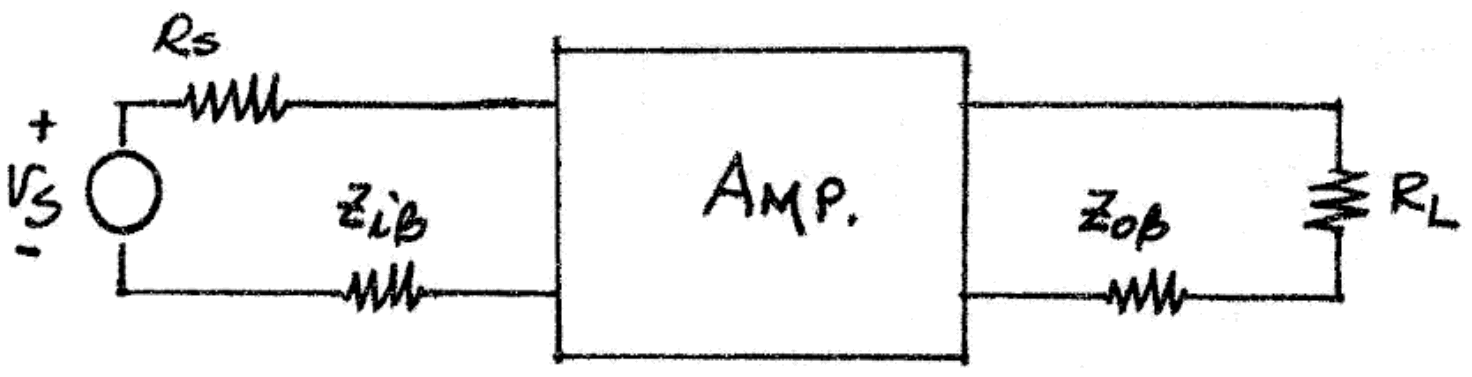
\includegraphics[width=0.44\linewidth]{_fig/retro_m-lazo_c-lazo_hallar-a.png}
		\label{fig:retro_m-lazo_c-lazo_hallar-a}
	}
	\subfloat[Definición de \(\beta\)]
	{
		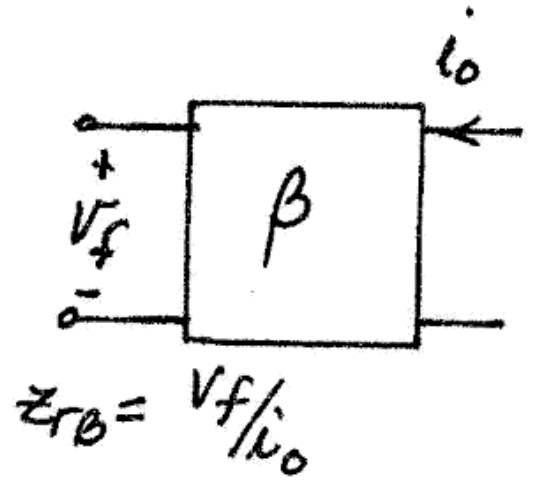
\includegraphics[width=0.44\linewidth]{_fig/retro_m-lazo_c-lazo_hallar-beta.png}
		\label{fig:retro_m-lazo_c-lazo_hallar-beta}
	}
	\caption{Formas para hallar \( A \) y \( \beta \)}
	\label{fig:retro_m-lazo_c-nodo_a-beta}
\end{figure}				

En la Figura \ref{fig:retro_m-lazo_c-lazo_hallar-beta}, el circuito para hallar \( \beta = Z_{o\beta}\), como la relación del voltaje a la entrada a \(V_s\) corriente de salida de la red de retroalimentación, con la entrada abierta.

\subsubsection{Ejemplo}

En las Figuras \ref{fig:retro_m-lazo_c-lazo_ejm-a} y \ref{fig:retro_m-lazo_c-lazo_ejm-b} se muestra un ejemplo de este tipo de retroalimentación. En la Figura \ref{fig:retro_m-lazo_c-lazo_ejm-b} se muestra cómo queda el amplificador sin retroalimentación, en la Figura \ref{fig:retro_m-lazo_c-lazo_ejm-c} la red de retroalimentación.

\begin{figure}[h]
	\centering
	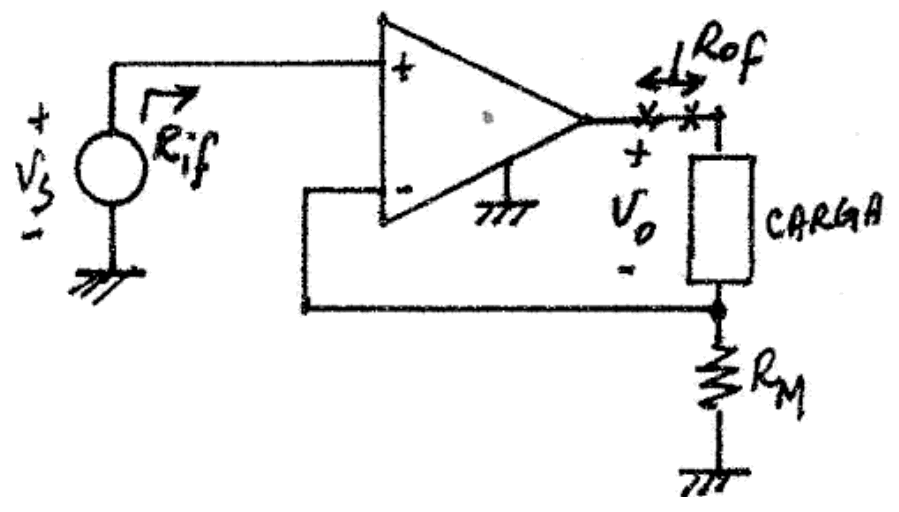
\includegraphics[width=0.8\linewidth]{_fig/retro_m-lazo_c-lazo_ejm-a.png}
	\caption{Ejemplos de retroalimentación: Amplificador}
	\label{fig:retro_m-lazo_c-lazo_ejm-a}
\end{figure}

\begin{figure}[h]
	\centering
	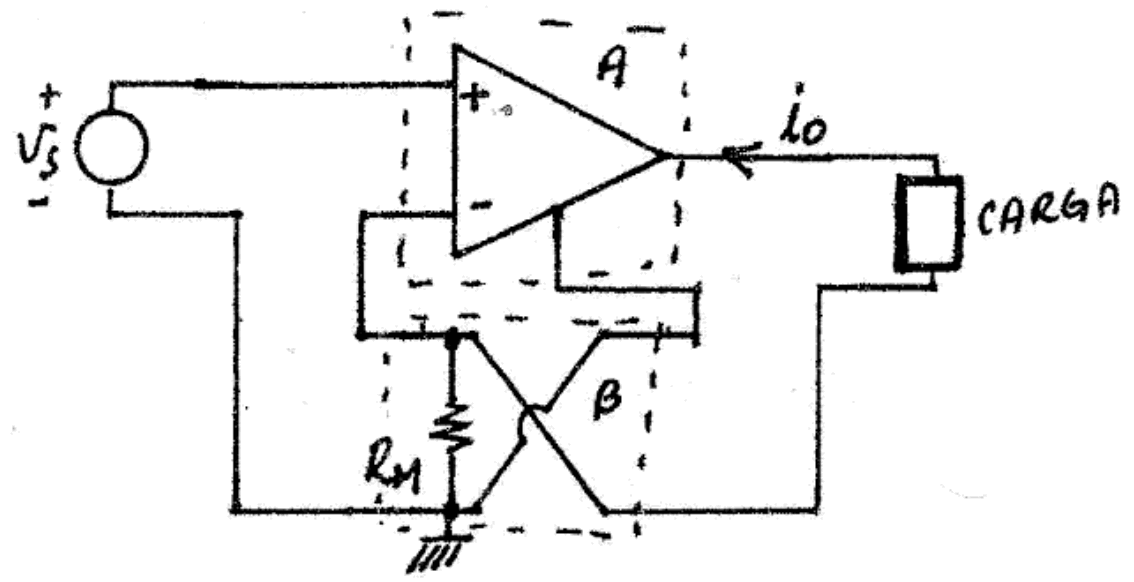
\includegraphics[width=0.8\linewidth]{_fig/retro_m-lazo_c-lazo_ejm-b.png}
	\caption{Ejemplos de retroalimentación: (b) Representación en cuadripolos}
	\label{fig:retro_m-lazo_c-lazo_ejm-b}
\end{figure}

\begin{figure}[h]
	\centering
	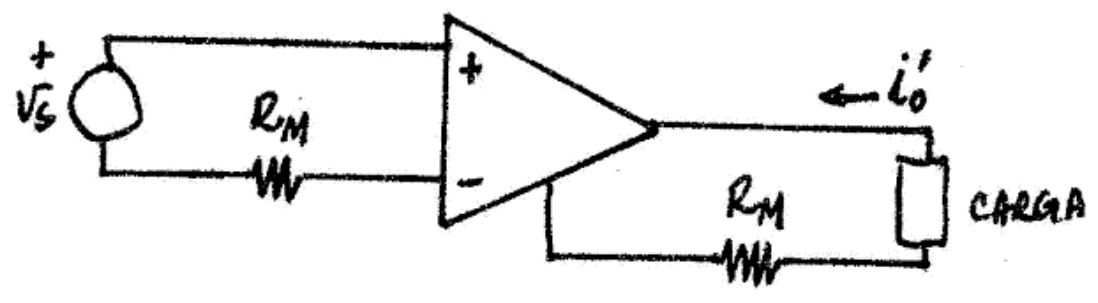
\includegraphics[width=0.6\linewidth]{_fig/retro_m-lazo_c-lazo_ejm-c.png}
	\caption{Ejemplos de retroalimentación: Amplificador sin retroalimentación}
	\label{fig:retro_m-lazo_c-lazo_ejm-c}
\end{figure}

\begin{figure}[h]
	\centering
	\includegraphics[width=0.3\linewidth]{_fig/retro_m-lazo_c-lazo_ejm-d.png}
	\caption{Ejemplos de retroalimentación: Red de retroalimentación}
	\label{fig:retro_m-lazo_c-lazo_ejm-d}
\end{figure}

\subsection{Muestreo de Nodo - Comparación de Lazo} %p161

\begin{figure}[h]
	\centering
	\includegraphics[width=0.8\linewidth]{_fig/retro_m-nodo_c-lazo.png}
	\caption{Muestreo de Nodo - Comparación de Lazo, Diagrama de Bloques}
	\label{fig:retro_m-nodo_c-lazo}
\end{figure}

En la Figura \ref{fig:retro_m-nodo_c-lazo}, se repite la Figura \ref{fig:retro_m-nodo_c-nodo} del diagrama de bloques general de este tipo de retroalimentación. En este caso el cuadripolo apropiado es el de los parámetros \( h \), que se muestra en la Figura \ref{fig:figura3.46}, ya que es el que tiene un nodo común a la salida y un lazo a la entrada.

\begin{figure}[h]
	\centering
	\includegraphics[width=0.8\linewidth]{_fig/retro_m-nodo_c-lazo_cuadripolo.png}
	\caption{Cuadripolo de parámetros \( h \).}
	\label{fig:retro_m-nodo_c-lazo_cuadripolo}
\end{figure}

Para el cuadripolo de los parámetros \( h \) se tiene:

\begin{equation}
	Vi = h_i I_i + h_r Vo \quad (3.23a)
\end{equation}

\begin{equation}
	I_2 = h_f I_i + h_o Vo \quad (3.23b)
\end{equation}

donde:

\( h_i = V_i / I_i \), con la salida en corto circuito.

\( h_r = V_i / V_o \), con la entrada abierta.

\( h_f = I_2 / I_i \), con la salida en corto circuito.

\( h_o = I_o / V_o \), con la entrada abierta.

Como en los casos anteriores, el manejo del análisis se simplifica tremendamente si se cumplen unas condiciones básicas:

\begin{equation}
	|h_i| \gg |h_f| \quad (3.24a)
\end{equation}

\begin{equation}
	|h_r| \gg |h_o| \quad (3.24b)
\end{equation}

\begin{equation}
	|h_i h_o| \gg |h_f h_r| \quad (3.24c)
\end{equation}

\begin{figure}[h]
	\centering
	\includegraphics[width=0.8\linewidth]{_fig/retro_m-nodo_c-lazo_calcular-a.png}
	\caption{Circuito para calcular \( A \) sin retroalimentación.}
	\label{fig:retro_m-nodo_c-lazo_calcular-a}
\end{figure}

En la Figura \ref{fig:retro_m-nodo_c-lazo_calcular-a} se muestra cómo queda el circuito para calcular \( A \) sin retroalimentación, donde \( h_i \beta = V_i \beta / I_i \beta \) con \( V_o \beta = 0 \) y 
\( h_o \beta = 	I_{2\beta} / V_{o\beta} \) con \( V_{i\beta} = 0 \). Entonces: \( A_f = \frac{V_o}{V_s} = \frac{A}{1 + A \beta} \), donde \( A = -\frac{h_f A}{h_i h_o}, \quad \beta = -h_r \beta \)

\subsubsection{Ejemplo} %p163

Como ejemplo, se muestra otro amplificador con retroalimentación en la Figura \ref{fig:retro_m-nodo_c-lazo_ejm1a}.

\begin{figure}[h]
	\centering
	\includegraphics[width=0.8\linewidth]{_fig/retro_m-nodo_c-lazo_ejm1a.png}
	\caption{Ejemplo}
	\label{fig:retro_m-nodo_c-lazo_ejm1a}
\end{figure}

\textbf{Análisis según la Metodología de Retroalimentación}

\textbf{Primero:} \textit{Identificación del tipo de retroalimentación}:

La retroalimentación se crea por medio de la rama \( R_f \). Esta rama llega al lazo de entrada, y por lo tanto es \textbf{comparación de lazo}. En la salida, se toma la señal de retroalimentación en el mismo nodo de salida, por lo tanto es \textbf{muestreo de nodo}, es decir, se muestrea la tensión de salida.

\textbf{Segundo:} \textit{Hallar el punto de operación}:

En continua queda el circuito que se muestra en la Figura 3.49.

Una primera ecuación surge de la malla formada por la resistencia de colector de \( Q1 \) y la resistencia de emisor de \( Q2 \):

\[ (I_{C1} - I_{E2} \beta) \cdot 0k = I_{E2} \cdot 1k + 0.7 \]

Despejando \( I_{E2} \) queda:

\[ I_{E2} = \frac{V_{CC} - 0.7}{R_{E2} + R_{C1} (\beta + 1)} = 0.637 \text{ mA} \]

\begin{figure}[h]
	\centering
	\includegraphics[width=0.8\linewidth]{_fig/retro_m-nodo_c-lazo_ejm1b.png}
	\caption{Circuito en DC de la Figura \ref{fig:retro_m-nodo_c-lazo_ejm1a}}
	\label{fig:retro_m-nodo_c-lazo_ejmb}
\end{figure}

Por otro lado, se convierte el circuito a la izquierda de la base de Q1 en su equivalente de Thevenin y se resuelve la malla resultante:

\[ 5.1 = \frac{80k I_{E1}}{\beta +1} + 0.7 + ( I_{E1} + \alpha I_{E2} 1.1k \]

Reemplazando la expresión de $I_{E2}$ de la ecuación anterior, se encuentra:

\[ I_{E1} = 435 \mu A \]

\[ I_{E2} = 3.28 mA \]

\begin{figure}[h]
	\centering
	\includegraphics[width=0.8\linewidth]{_fig/retro_m-nodo_c-lazo_ejm1c.png}
	\caption{Circuito sin retroalimentación, parte A}
	\label{fig:retro_m-nodo_c-lazo_ejmc}
\end{figure}

\begin{figure}[h]
	\centering
	\includegraphics[width=0.8\linewidth]{_fig/retro_m-nodo_c-lazo_ejm1d.png}
	\caption{Circuito sin retroalimentación, parte B}
	\label{fig:retro_m-nodo_c-lazo_ejmd}
\end{figure}

\textbf{Tercero:} Con estos valores de los puntos de operación se pueden calcular los valores de los parámetros de los transistores. Se elimina la red de retroalimentación para dejar el amplificador sin retroalimentación, al cual se anexa a la entrada y a la salida el efecto de carga de la red de retroalimentación. El resultado se muestra en la Figura \ref{fig:retro_m-nodo_c-lazo_ejmc}, con su circuito equivalente a frecuencias medias en la Figura \ref{fig:retro_m-nodo_c-lazo_ejmd}.

Aqui se ha transformado \( R_{s} \) y las resistencias de polarización \( R_{B1} \) y \( R_{B2} \) junto con la fuente \( V_{s} \) en su equivalente de Thevenin con \( R_{s}^{\prime} \) y \( V_{s}^{\prime} \) para llegar a la configuración de la Fig. \ref{fig:retro_m-nodo_c-lazo_c}. De aqui procedemos normalmente para obtener:

\[A = \frac{v_{o}^{\prime}}{v_{s}^{\prime}} = 89.6\]

\[R_{i} = R_{s}^{\prime} + r_{\pi} + (\beta + 1) 93.75 = 16041 \Omega\]

\[R_{o} = 1.6 k\Omega\]

\begin{figure}[h]
	\centering
	\includegraphics[width=0.5\linewidth]{_fig/retro_m-nodo_c-lazo_ejm1e.png}
	\caption{Circuito para determinar $\beta$}
	\label{fig:retro_m-nodo_c-lazo_ejme}
\end{figure}				
\textbf{Cuarto:}  La red de retroalimentación está formada por \( R_{EM} \) y \( R_{f} \), tal como se muestra en la Figura \ref{fig:retro_m-nodo_c-lazo_ejme}. \( \beta \) viene dada por \( \frac{v_{f}}{v_{o}} = \frac{R_{EM}}{R_{EM} + R_{f}} = \frac{100}{100 + 1500} = 0.0625 \)

\textbf{Quinto:}  Finalmente, una vez conocido todos los valores sin retroalimentación, se procede a calcular los valores con retroalimentación, y \( \beta \) se pueden determinar las características del circuito con retroalimentación. Tenemos:

\[ D = 1 + A\beta = 6.6 \]

\[ A_f = A/D = 13.6 \]

\[ R_{if} = R_i D = 106 k\Omega \]

\[ R_{of} = R_o / D = 242 \Omega \]

En la consideración final se encuentra el valor de la resistencia de entrada después de la fuente, $R_i^{\prime}$. Haciendo referencia a la ecuación desarrollada en la discusión de este tipo de retroalimentación, se obtiene:

\[ R_i^{\prime} = 105 k\Omega \quad R_{out} = 390k // 100k // 105k = 45.3 k\Omega \]

\subsection{Muestreo de Lazo - Comparación de Nodo} %p166

El último caso a considerar es la retroalimentación Muestreo de Lazo - Comparación de Nodo. En la Figura \ref{fig:retro_m-lazo_c-nodo}, se repite la Figura \ref{fig:retro_m-lazo_c-nodo_a} del diagrama de bloques general de este tipo de retroalimentación. En este caso el cuadripolo apropiado es el de los parámetros \( g \), que se muestra en la Figura \ref{fig:retro_retro_m-lazo_c-nodo_cuadripolo}, ya que es el que tiene un nodo común a la salida y un lazo a la entrada.

\begin{equation}
	I_1 = V_1 g_{11} + I_2 g_{12}
\end{equation}

\begin{figure}[h]
	\centering
	\includegraphics[width=0.8\linewidth]{_fig/retro_m-lazo_c-nodo.png}
	\caption{Muestreo de Lazo - Comparación de Nodo, Diagrama de Bloques}
	\label{fig:retro_m-lazo_c-nodo}
\end{figure}

\begin{figure}[h]
	\centering
	\includegraphics[width=0.6\linewidth]{_fig/retro_m-lazo_c-nodo_cuadripolo.png}
	\caption{Cuadripolo de parámetros \( g \).}
	\label{fig:retro_retro_m-lazo_c-nodo_cuadripolo}
\end{figure}

Para el cuadripolo de los parámetros \( g \) se tiene:

\begin{equation}
	V_2 = g_f V_i + g_o I_o
\end{equation}

Igual a los casos anteriores, el manejo del análisis se simplifica tremendamente si se cumplen unas condiciones básicas:

\begin{equation}
	|g_{fA}| >> |g_{f\beta}|
\end{equation}

\begin{equation}
	|g_{r\beta}| >> |g_{rA}|
\end{equation}

\begin{equation}
	|G_i G_o| >> |g_{fA} g_{rA}|
\end{equation}

\begin{figure}[h]
	\centering
	\includegraphics[width=0.6\linewidth]{_fig/retro_retro_m-lazo_c-nodo_calcular-a.png}
	\caption{Cuadripolo de parámetros \( g \).}
	\label{fig:retro_retro_m-lazo_c-nodo_calcular-a}
\end{figure}

En la Figura \ref{fig:retro_retro_m-lazo_c-nodo_calcular-a} se muestra cómo queda el circuito para calcular \( A \) sin retroalimentación. Entonces \( A_f = \frac{I_o}{V_s} = \frac{A}{(1 + A\beta)} \), donde \( A = \frac{-g_{fA}}{H_i H_o} \) y \( \beta = -g_r \beta \)

\subsubsection{Ejemplo} %p167

\begin{figure}[h]
	\centering
	\includegraphics[width=0.8\linewidth]{_fig/retro_m-lazo_c-nodo_ejm1a.png}
	\caption{Circuito de ejemplo}
	\label{fig:retro_m-lazo_c-nodo_ejm1a}
\end{figure}

Ahora resolveremos un ejemplo con este tipo de retroalimentación, que se muestra en la Figura \ref{fig:retro_m-lazo_c-nodo_ejm1a}.

\textbf{Primero:} identificar el tipo de retroalimentación: la retroalimentación se crea por medio de la rama Rf. Esta rama llega al mismo nodo de entrada, y por lo tanto es comparación de nodo. En la salida, la tensión en Re2 nos da una muestra del valor de la corriente en el lazo de salida, y por lo tanto es muestreo de lazo.

\textbf{Segundo:} Hallar el punto de operación. En continua queda el circuito que se muestra en la Figura \ref{fig:retro_m-lazo_c-nodo_ejm1a}.

\begin{figure}[h]
	\centering
	\includegraphics[width=0.5\linewidth]{_fig/retro_m-lazo_c-nodo_ejm1b.png}
	\caption{Circuito en DC de la Figura \ref{fig:retro_m-lazo_c-nodo_ejm1a}}
	\label{fig:retro_m-lazo_c-nodo_ejm1b}
\end{figure}

Aplicando el procedimiento de costumbre, con \( \beta = 130 \), \(r_T = 3.4k\Omega \), se obtiene:

\[
(V_{CE1}, I_{C1}) \approx (1.2V, 1mA)
\]

\[
(V_{CE2}, I_{C2}) \approx (3.5V, 1.06mA)
\]

\textbf{Tercero:} Con estos valores de los puntos de operación se pueden calcular los valores de los parámetros de los transistores. Se elimina la red de retroalimentación para dejar el amplificador sin retroalimentación, al cual se anexa a la entrada y a la salida el efecto de carga de la red de retroalimentación. El resultado se muestra en la Figura \ref{fig:retro_m-lazo_c-nodo_ejm1c}, con su circuito equivalente a frecuencias medias en la Figura \ref{fig:retro_m-lazo_c-nodo_ejm1d}.

\begin{figure}[h]
	\centering
	\includegraphics[width=0.8\linewidth]{_fig/retro_m-lazo_c-nodo_ejm1c.png}
	\caption{Circuito sin retroalimentación. Parte 1}
	\label{fig:retro_m-lazo_c-nodo_ejm1c}
\end{figure}

\begin{figure}[h]
	\centering
	\includegraphics[width=0.8\linewidth]{_fig/retro_m-lazo_c-nodo_ejm1d.png}
	\caption{Circuito sin retroalimentación. Parte 2}
	\label{fig:retro_m-lazo_c-nodo_ejm1d}
\end{figure}

Se hace notar que hemos convertido la fuente de entrada, junto con su resistencia, en el equivalente de Norton por considerarse de una retroalimentación tipo comparación de nodo. De aquí procedemos normalmente para obtener:

\[ A = \frac{i_o^{''}}{i_s} = -503 \]

\[ R_i\prime = 1785 \]

\[ R_o = \infty \]

De querer la respuesta de frecuencia sin retroalimentación, se volverían a colocar los condensadores para frecuencias bajas, y para altas se trabajaría con el modelo de alta del transistor.

\textbf{Cuarto:} La red de retroalimentación está formada por $R_f$ y $R_{E2}$. El factor de retroalimentación $\beta$ viene dado por $\frac{i_f}{i_o}$. Sin embargo, se hace notar que la corriente que circula por $R_{E2}$ no es exactamente la corriente de salida $i_o$, por dos motivos: la corriente de emisor es ligeramente mayor que la corriente de colector, y además, la corriente de colector es la suma de la corriente de salida más la corriente que circula por la resistencia de colector. En la Figura \ref{fig:retro_m-lazo_c-nodo_ejm1e_a} se muestra propiamente la red de retroalimentación; de aquí se obtiene \( \frac{i_f}{i_o}\prime = \frac{R_{E2}}{R_{E2}+R_f} \). En la figura \ref{fig:retro_m-lazo_c-nodo_ejm1e_b} se muestra la etapa de salida para determinar la relación entre la corriente de salida $i_o$ y l acorriente de emisor. Entonces la relación entre la corriente de salida y la corriente de retroalimentación, es decir, $\beta$ viene dada por:

\[ \frac{i_f}{i_o} = (-0.107)(1.15) = -0.123	\]

\begin{figure}[h]
	\centering
	\subfloat[A]
	{
		\includegraphics[width=0.5\linewidth]{_fig/retro_m-lazo_c-nodo_ejm1e_a.png}
		\label{fig:retro_m-lazo_c-nodo_ejm1e_a}
	}
	\subfloat[B]
	{
		\includegraphics[width=0.3\linewidth]{_fig/retro_m-lazo_c-nodo_ejm1e_b.png}
		\label{fig:retro_m-lazo_c-nodo_ejm1e_b}
	}
	\caption{Circuitos para determinar $\beta$}
	\label{fig:retro_m-lazo_c-nodo_ejm1e}
\end{figure}

\textbf{Quito:} Finalmente, una vez conocidos todos los valores sin retroalimentación y \( \beta \), se pueden determinar las características del circuito con retroalimentación. Tenemos:

\[ D = 1 + A\beta = 62.7 \]

\[ A_f = \frac{A}{D} = -8 \]

\[ R_{if} = \frac{R_i}{D} = 28.4 \]

\[ R_{of} = R_o D = \infty \]

\[ \frac{v_o}{v_s} = -\frac{i_o R_L}{i_s R_s} = \frac{-A_f R_L}{R_s} = 0.8 \]

En los ajustes finales se encuentran valores de las características de mayor interés, como son la resistencia de entrada después de la fuente, \( R_i' \) y la resistencia de salida total, $R_{sal}'$. Haciendo referencia a las ecuaciones desarrolladas en la discusión de este tipo de retroalimentación, se obtiene:

\[ R_i\prime = \frac{1}{\frac{1}{28.4} - \frac{1}{10k}} = 28.5 \Omega \]

\[ R_{sal} = 1k \parallel 6.8k = 872 \Omega \]

\subsection{Resumen} %p171

Si se satisfacen las condiciones de que la amplificación es principalmente por el amplificador, y que la retroalimentación es principalmente por la red de retroalimentación, como por ejemplo en las ecuaciones \ref{equ:retro_m-nodo_c-nodo_admitancia-yfA}, \ref{equ:retro_m-nodo_c-nodo_admitancia-yfB} y 			\ref{equ:retro_m-nodo_c-nodo_admitancias}, entonces puede utilizarse la Metodología de Retroalimentación que consta de los siguientes pasos:

\begin{enumerate}
	\item Identificación del tipo de retroalimentación.
	\item Generalmente se tiene que encontrar el punto de operación, para el cual se trabaja con el circuito original, sin modificaciones.
	\item Formación del amplificador sin retroalimentación, del cual se determina la ganancia sin retroalimentación, \( A \), la resistencia de entrada sin retroalimentación, \( R_{if} \), la resistencia de salida sin retroalimentación, \( R_{of} \), y las frecuencias de corte baja y corte alta sin retroalimentación, \( f_L \) y \( f_H \) respectivamente.
	\item El cálculo de \( \beta \) de acuerdo a los lineamientos que se han dado.
	\item El cálculo de las características del circuito con retroalimentación de acuerdo a las siguientes relaciones:
\end{enumerate}

\begin{equation}
	A_f = \frac{A}{1 + A\beta}
\end{equation}

\begin{equation}
	R_{if} =
	\begin{cases} 
		R_i/(1 + A\beta) & \text{si es comparación de nodo} \\
		R_i(1 + A\beta) & \text{si es comparación de lazo}
	\end{cases}
\end{equation}

\begin{equation}
	R_{of} =
	\begin{cases} 
		R_o/(1 + A\beta) & \text{si es muestreo de nodo} \\
		R_o(1 + A\beta) & \text{si es muestreo de lazo}
	\end{cases}
\end{equation}

\begin{equation}
	f_{Lf} = \frac{f_L}{1 + A\beta}
\end{equation}

\begin{equation}
	f_{Hf} = f_H (1 + A\beta)
\end{equation}

\section{Determinación de configuraciones de retroalimentación positiva} %p171

En ocasiones se presentan configuraciones que tienen retroalimentación, pero de tal forma que en lugar de restar el nivel de la señal de entrada, más bien lo aumentan. Esto corresponde a una situación inestable, se entra en un círculo vicioso ya que la misma señal realimentada aumenta la entrada, que aumenta la señal de salida y así sucesivamente.

Una forma de determinar si una configuración tiene retroalimentación positiva o negativa consiste en encontrar valores de \( A \) y \( \beta \) siguiendo los procedimientos que hemos formulado, y comparar los signos de \(A\) y \(\beta\):

\begin{itemize}
	\item Si son iguales, tenemos retroalimentación negativa.
	\item Si son opuestos, tenemos retroalimentación positiva.
\end{itemize}

Sin embargo, para comprobaciones rápidas se propone otra manera, que a su vez, nos da una concepción más intuitiva de por qué la retroalimentación negativa le imparte una estabilidad a un sistema.

El método consiste en abrir el lazo de retroalimentación en cualquier punto y aplicar una fuente imaginaria a ese punto; se hace un seguimiento de esta señal alrededor del lazo, y si al regresar al punto de partida, es decir, el punto donde se abrió el lazo, la señal está en contrafase, tenemos un caso de retroalimentación negativa. Si, en cambio, la señal que retorna está en fase con la señal aplicada, entonces tenemos retroalimentación positiva.

Este método se demuestra aplicado a los circuitos de la Figura \ref{fig:retro_pos_ejm1}.

\begin{figure}[h]
	\centering
	\subfloat[Paso 1]
	{
		\includegraphics[width=0.22\linewidth]{_fig/retro_pos_ejm1a.png}
		\label{fig:retro_pos_ejm1a}
	}
	\subfloat[Paso 2]
	{
		\includegraphics[width=0.22\linewidth]{_fig/retro_pos_ejm1b.png}
		\label{fig:retro_pos_ejm1b}
	}
	\subfloat[Paso 3]
	{
		\includegraphics[width=0.22\linewidth]{_fig/retro_pos_ejm1c.png}
		\label{fig:retro_pos_ejm1c}
	}
	\subfloat[Paso 4]
	{
		\includegraphics[width=0.22\linewidth]{_fig/retro_pos_ejm1d.png}
		\label{fig:retro_pos_ejm1d}
	}
	\caption{Ejemplo 1: circuito con transistores}
	\label{fig:retro_pos_ejm1}
\end{figure}

En el circuito de la figura \ref{fig:retro_pos_ejm1a}, abrimos el lazo en el punto marcado con $x$. Se aplica una fuente de tensión al emisor de $Q_1$; el circuito queda como se muestra en la figura \ref{fig:retro_pos_ejm1a}. De esta forma, $Q_1$ queda como una base común, en donde de emisor a colector no hay inversión de fase. Luego, desde el colector de $Q_1$ (base de $Q_2$ al emisor de $Q_2$ tampoco hay inversión de fase. Finalmente, a través de la resistencia $R_f$ tampoco hay inversión de fase. Concluimos que la señal está en fase con la señal aplicada, indicando retroalimentación positiva.

Analice los demás circuitos de la figura \ref{fig:retro_pos_ejm1} y determine si son de retroalimentación positiva o negativa.

Finalmente, si se carga apropiadamente el lazo con la resistencia que vería la señal al seguir dando la vuelta al lazo, y se encuentra la relación entre la señal retornada a la señal aplicada, \( \frac{V_r}{V_a} \); se ha encontrado la \textbf{ganancia del lazo}, $A\beta$. La ganancia de lazo es muy utilizada para determinar la estabilidad de un sistema. Esto se realiza al circuito de la figura \ref{fig:retro_pos_ejm2a} para llegar a la figura \ref{fig:retro_pos_ejm2b}.

\begin{figure}[h]
	\centering
	\subfloat[Circuito con retroalimentación]
	{
		\includegraphics[width=0.4\linewidth]{_fig/retro_pos_ejm2a.png}
		\label{fig:retro_pos_ejm2a}
	}
	\subfloat[Análisis de retroalimentación]
	{
		\includegraphics[width=0.5\linewidth]{_fig/retro_pos_ejm2b.png}
		\label{fig:retro_pos_ejm2b}
	}
	\caption{Ejemplo 2: circuito y analisis}
	\label{fig:retro_pos_ejm2}
\end{figure}

\textbf{Bibliografía:}

\begin{itemize}
	\item Millman, Halkias, \textit{Electrónica Integrada}, McGraw-Hill, 1972, Capítulo 13.
	\item Gray, Searle, \textit{Principios de Electrónica}, Wiley and Sons, 1969, Capítulo 18.
	\item Sedra, Smith, \textit{Microelectronic Circuits}, Holt-Saunders International Edition, New York, 1982, Capítulo 12.
\end{itemize}

\section{Problemario} %p175
- pendiente en apuntes -	% Retroalimentación
	% Licencia y derechos: consulte ../../LICENSE-CC-BY-4.0.
% Las figuras y demás materiales de terceros pueden tener derechos separados y deben identificarse.

\chapter{Estabilidad y osciladores} %p183
\section{Introducción} %p183
Un oscilador es un sistema que genera una señal periódica. Esquemáticamente se representa en la Figura \ref{fig:osc_basic}.

\begin{figure}[h]
	\centering
	\includegraphics[width=0.7\linewidth]{_fig/osc_basic.pdf}
	\caption{Un oscilador}
	\label{fig:osc_basic}
\end{figure}

Se distingue entre los generadores de onda sinusoidal, y los generadores de onda cuadrada o rectangular. Generalmente, los osciladores generadores de onda sinusoidal se implementan en dispositivos electrónicos trabajando de forma lineal, mientras los generadores de onda cuadrada o rectangular trabajan los dispositivos en forma no-lineal. Por ahora, nos interesa los osciladores que generan ondas sinusoidales, es decir, estaremos trabajando con dispositivos que trabajan en forma lineal. La discusión de generadores de onda cuadrada o rectangular tiene un enfoque notablemente distinto.

El esquema de la Figura \ref{fig:osc_basic} se ha omitido la fuente de polarización que energiza el sistema. En la Figura  \ref{fig:osc_basic-dc} se indica esta fuente de DC. Esta figura destaca otra interpretación del oscilador, que es de un convertidor de corriente continua a corriente alterna. En cualquier caso, el oscilador es un sistema no-lineal, bien esta porque genera una frecuencia de salida que no es suministrada por la entrada (la fuente DC), o porque la genera sin tener entrada (la fuente DC sólo polariza el circuito). Se podría considerar como un sistema marginalmente estable, ya que la amplitud de la señal no aumenta ni disminuye con el tiempo.

\begin{figure}[h]
	\centering
	\includegraphics[width=0.7\linewidth]{_fig/osc_basic-dc.pdf}
	\caption{Un oscilador, polarizado con una fuente DC}
	\label{fig:osc_basic-dc}
\end{figure}

Un sistema que genera una señal sinusoidal es marginalmente estable y tiene sus polos sobre el eje imaginario; su función de transferencia podría ser de la siguiente forma:

\( H(s) = \frac{a}{s^2 + a^2} \), con polos en \( s^2 = -a^2 \), es decir, \( s = \pm ja \)

Tal como se indica en la Figura \ref{fig:osc_sine_polos-y-ceros}, la frecuencia de oscilación es \( a \).

\begin{figure}[h]
	\centering
	\includegraphics[width=0.7\linewidth]{_fig/osc_sine_polos-y-ceros.png}
	\caption{Diagrama de polos y ceros de onda sinusoidal}
	\label{fig:osc_sine_polos-y-ceros}
\end{figure}

Hay ocasiones cuando queremos un circuito que oscile a una determinada frecuencia. Pero también hay la posibilidad que un circuito oscile cuando no deseamos ese comportamiento; por ejemplo, hay configuraciones de amplificadores de alta ganancia que "estallan" en oscilaciones permanentes.

Estos dos casos están relacionados. En este tema vamos a querer aprender lo siguiente: ¿Por qué oscila un circuito? ¿Cómo evitar que un circuito oscile cuando no lo deseamos? ¿Cómo diseñar un circuito para que oscile a una determinada frecuencia?

\subsection{Ejemplo}
\begin{figure}[h]
	\centering
	\includegraphics[width=0.7\linewidth]{_fig/osc_ejm1.png}
	\caption{Circuito de tres etapas con retroalimentación}
	\label{fig:osc_ejm1}
\end{figure}

Uno de los circuitos que se vio en el tema de retroalimentación fue la configuración de tres etapas con muestreo de nodo - comparación de nodo que se muestra en la Figura \ref{fig:osc_ejm1}. En principio, es una configuración de retroalimentación negativa. Sin embargo, se montó en el laboratorio y empezó a oscilar. ¿Qué pasó?

\begin{figure}[h]
	\centering
	\includegraphics[width=0.7\linewidth]{_fig/osc_ejm1_alta-frecuencia.png}
	\caption{Modelo de alta frecuencia de la Figura \ref{fig:osc_ejm1}}
	\label{fig:osc_ejm1_alta-frecuencia}
\end{figure}

Recordemos que la retroalimentación negativa exige que \( A \) y \( B \) tengan el mismo signo \( - \) y en efecto, a frecuencias medias, el circuito de arriba cumple con esta condición. Sin embargo, al considerar la ganancia del amplificador sin retroalimentación, y el modelo de alta frecuencia del transistor, como se muestra en la Figura \ref{fig:osc_ejm1_alta-frecuencia}, el circuito presenta polos de alta frecuencia. En una aproximación de primer orden, se asocia un polo dominante por cada transistor, de modo que el circuito tiene tres polos. Cada polo introduce un desfase que es de \( 0^\circ \) a frecuencias bajas y medias, y llega a un valor mínimo de \( -90^\circ \). Por lo tanto, si se consideran los tres polos, van a cambiar el desfase inicial de \( A \) por la cantidad de \( -270^\circ \); en particular, lo llegan a cambiar por \( -180^\circ \), lo que representa un cambio de signo. 

Por lo tanto, si a frecuencias medias \( A \) y \( \beta \) son del mismo signo, a otra frecuencia superior serán de signo opuesto, y el sistema que cumple con las condiciones de retroalimentación negativa a frecuencias medias, se convierte en un sistema de retroalimentación positiva, provocando una inestabilidad que puede manifestarse en la forma de oscilaciones.

En este tema queremos estudiar esta condición de oscilación, bien sea para evitarla, tal vez con una compensación de frecuencia, o para buscarla y así crear el tipo de circuito conocido como oscilador.

Una técnica gráfica que indica el comportamiento oscilatorio de un sistema al ser sometido a retroalimentación es \textbf{el lugar geométrico de las raíces}. En principio, la función de transferencia del amplificador viene dada por \( A(s) \). Al someter el amplificador a una retroalimentación \( \beta \), surge la función de transferencia del amplificador con retroalimentación:

\begin{equation}
	A_f(s) = \frac{A(s)}{1 + A(s)\beta}
\end{equation}

Evidentemente, las raíces del sistema cambiarán; además, su ubicación será función del valor de \( \beta \). Por lo tanto, la técnica del lugar geométrico de las raíces describe la trayectoria de las raíces del sistema a medida que \( \beta \) aumenta.

Consideramos tres casos por ahora:
sistemas sin retroalimentación de un polo real y negativo,
dos polos reales y negativos,
y tres polos reales y negativos 

\begin{figure}[h]
	\centering
	\subfloat[1 polo]
	{
		\includegraphics[width=0.3\linewidth]{_fig/osc_3roots-1.png}
		\label{fig:osc_3roots-1}
	}
	\subfloat[2 polos]
	{
		\includegraphics[width=0.3\linewidth]{_fig/osc_3roots-2.png}
		\label{fig:osc_3roots-2}
	}
	\subfloat[3 polos]
	{
		\includegraphics[width=0.3\linewidth]{_fig/osc_3roots-3.png}
		\label{fig:osc_3roots-3}
	}
	\caption{Lugar geométrico de raíces de 3 sistemas}
	\label{fig:osc_3roots}
\end{figure}

\begin{figure}[h]
	\centering
	\subfloat[1 polo]
	{
		\includegraphics[width=0.3\linewidth]{_fig/osc_3roots-1-wt.png}
		\label{fig:osc_3roots-1-wt}
	}
	\subfloat[2 polos]
	{
		\includegraphics[width=0.3\linewidth]{_fig/osc_3roots-2-wt.png}
		\label{fig:osc_3roots-2-wt}
	}
	\subfloat[3 polos]
	{
		\includegraphics[width=0.3\linewidth]{_fig/osc_3roots-3-wt.png}
		\label{fig:osc_3roots-3-wt}
	}
	\caption{Lugar geométrico de raíces de 3 sistemas, con trazas}
	\label{fig:osc_3roots-wt}
\end{figure}

Se muestran en las Figuras \ref{fig:osc_3roots-1}, \ref{fig:osc_3roots-2} y \ref{fig:osc_3roots-3}. En las Figuras \ref{fig:osc_3roots-1-wt}, \ref{fig:osc_3roots-2-wt} y \ref{fig:osc_3roots-3-wt} respectivamente, se traza la trayectoria de las raíces a medida que aumenta \( \beta \).

En el sistema de un solo polo, la Figura \ref{fig:osc_3roots-1}, a medida que aumenta \( \beta \), este polo se desplaza hacia la izquierda por el mismo eje real, la Figura \ref{fig:osc_3roots-1-wt}. Esto quiere decir que cuanto más retroalimentación tiene el sistema, mayor es su ancho de banda.

En base a funciones de transferencia, tenemos la del sistema sin retroalimentación:

\begin{equation}
	A(s) = \frac{A_0}{1 + j\frac{f}{f_H}}
\end{equation}

Con la cual se obtiene la del sistema con retroalimentación:

\begin{equation}
	A_f(s) = \frac{A_0}{1 + \beta A_0 + j\frac{f}{f_H}}
\end{equation}

De donde concluimos que la frecuencia de corte con retroalimentación en función de la frecuencia de corte sin retroalimentación viene dada por:

\begin{equation}
	f_{H\beta} = f_H (1 + A_0\beta)
\end{equation}

Lo cual demuestra lo dicho relativo al ancho de banda, se hace notar que la retroalimentación no modifica el producto ganancia-ancho de banda del sistema: en la medida que disminuye la ganancia, así mismo aumenta el ancho de banda.

En el sistema de dos polos, la Figura \ref{fig:osc_3roots-2}, a medida que aumenta \( \beta \), estos polos primero se acercan por el mismo eje real, y al encontrarse, se despegan del eje real en forma perpendicular a él, con una parte real constante y una parte imaginaria crecientemente más grande, la Figura \ref{fig:osc_3roots-2-wt}. Cuando la parte imaginaria supera en valor absoluto a la parte real, la respuesta de frecuencia tiene una resonancia que se hace más pronunciada a medida que aumenta la parte imaginaria, es decir, a medida que aumenta \( \beta \). Sin embargo, los polos permanecen en el plano izquierdo y el sistema es siempre estable.

Si la función de transferencia del sistema sin retroalimentación se expresa como:

\begin{equation}
	A(s) = \frac{A_0}{(1 + s/w_1)(1 + s/w_2)}
\end{equation}

Entonces la función de transferencia del sistema con retroalimentación viene dada por:

\begin{equation}
	A_f(s) = \frac{A_0 w_1 w_2}{s^2 + (w_1 + w_2)s + w_1 w_2 (1 + \beta A_0)}
\end{equation}

\begin{figure}[h]
	\centering
	\subfloat[Respuesta de frecuencia]
	{
		\includegraphics[width=0.45\linewidth]{_fig/osc_sys-2-polos-freq.png}
		\label{fig:osc_sys-2-polos-frec}
	}
	\subfloat[Respuesta a un escalón]
	{
		\includegraphics[width=0.45\linewidth]{_fig/osc_sys-2-polos-step.png}
		\label{fig:osc_sys-2-polos-step}
	}
	\caption{Sistema de dos polos}
	\label{fig:osc_sys-2-polos}
\end{figure}

En la Figura \ref{fig:osc_sys-2-polos} se muestra la respuesta de frecuencia y la respuesta a un escalón de sistemas de segundo orden en función de la calidad, \( Q \), del sistema.

En un sistema de tres polos, la Figura \ref{fig:osc_3roots-3}, a medida que aumenta la retroalimentación, el polo a la izquierda se va alejando del origen por el mismo eje real, y los dos polos más cerca al origen se acercan y se despegan con una trayectoria que se aproximan a asíntotas que hacen ángulos de \( \pm 60^\circ \) con el eje real, la Figura \ref{fig:osc_3roots-3-wt}. Con estas trayectorias se destaca que dado suficiente retroalimentación, los polos cruzan el eje imaginario y pasan al plano derecho. Entonces el sistema, que era estable en principio, puede convertirse en un sistema inestable dada suficiente retroalimentación. Dada la función de transferencia del sistema sin retroalimentación:

\begin{equation}
	A(s) = \frac{A_0}{(1 + s/w_1)(1 + s/w_2)(1 + s/w_3)}
\end{equation}

La función del sistema con retroalimentación puede expresarse como:

\begin{equation}
	A_f(s) = \frac{A_0}{\left[ \left(\frac{s}{w_0}\right)^3 + a_2 \left(\frac{s}{w_0}\right)^2 + a_1 \left(\frac{s}{w_0}\right) + 1 \right]}
\end{equation}

Finalmente, otro enfoque para entender las condiciones de oscilación analiza la expresión de la ganancia con retroalimentación:

\begin{equation}
	A_f = \frac{A}{1 + A\beta}
\end{equation}

Evidentemente, si \( A\beta = -1 \), la ganancia tiende a \( \infty \) y el sistema es inestable. La relación \( A\beta = -1 \), o también \( -A\beta = 1 \), es conocida como el criterio de \textbf{Barkhausen} para que un sistema oscile. La expresión \( -A \beta \) es la \textbf{ganancia de lazo} que presentamos en el tema anterior y representa la relación entre una señal aplicada en cualquier punto del lazo, y la señal que regresa a ese punto alrededor del lazo. Si esta ganancia es igual a uno con cero desfasaje tenemos un oscilador. Ver la Figura \ref{fig:osc_ganancia-lazo}.

\begin{figure}[h]
	\centering
	\includegraphics[width=0.8\linewidth]{_fig/osc_ganancia-lazo.png}
	\caption{Ganancia del lazo \( = -A \beta \)}
	\label{fig:osc_ganancia-lazo}
\end{figure}

\section{Estabilidad} %190

Hemos visto que existe el riesgo de oscilación al introducir retroalimentación en amplificadores conformados con al menos 3 etapas. En el diseño de amplificadores es necesario asegurar que el circuito sea estable a todas las frecuencias, y no limitarse a cierto rango de interés.

Esto exige que los polos de la función de transferencia, es decir, los ceros de \( 1 + A\beta \) se encuentren en el plano izquierdo. Hay otros criterios que también permiten determinar la estabilidad de un sistema con retroalimentación.

\subsection{El criterio de Nyquist} %p190

Se grafica el número complejo \( A\beta \) en el plano complejo para \( f \) entre \( -\infty \) y \( +\infty \). Si la curva resultante encierra el punto \( -1+j0 \), el amplificador es inestable; si no lo encierra, entonces es estable.

\textbf{Ejemplo:} Si tenemos un sistema de un solo polo:

\[
\beta A = \frac{\beta A_0}{(1+jf/f_H)} = \frac{\beta A_0 (1 - jf/f_H)}{1+(f/f_H)^2}
\]

Dejando que \( A_0 = 1000 \), \( f_H = 2000 \), \( \beta = 0.1 \), las expresiones para las partes real e imaginaria de \( \beta A \) son:

\[
\text{Re}|\beta A| = \frac{\beta A_0}{1 + (f/f_H)^2} = \frac{100}{1 + (f/2000)^2}
\]

\[
|\text{Im}[\beta A]| = \frac{-\beta A_0 f}{f_H [1+(f/f_y)^2]} = \frac{100f}{2000[1+(f/2000)^2]}
\]

Sustituyendo valores se obtienen los siguientes resultados; se hace notar que para $f$ negativo cambia el signo con respecto al resultado para $f$ positivo; se grafican en la Figura \ref{fig:osc_ab-plano-complejo}. La curva inferior es para $f$ positivo, y la superior, el imagen espejo de la inferior, es para $f$ negativo. Como "$-1$" no está en el interior (definido como a la izquierda \textit{cuando se va de $-\infty$ a $+\infty$}) de la forma, entonces es un sistema estable.

\begin{tabular}{c|cccccccccc}
	$f$     & 10  & 100 & 1000 & 2000 & 3000 & 4000 & 5000 & 10k  & 100k \\
	Re$[\beta A]$ & 100 & 99.7 & 88   & 50   & 30.7 & 20   & 13.8 & 3.85 & 0.04 \\
	Im$[\beta A]$ & -0.5& -4.9 & -40  & -50  & -46  & -40  & -34  & -19  & -2 \\
\end{tabular}

%			\begin{table}[H]
	%				\centering
	%				\caption*{Valores de $\text{Re}[\beta A]$ y $\text{Im}[\beta A]$ para $f>0$}
	%				\begin{tabular}{c|cccccccccc}
		%					$f$     & 10  & 100 & 1000 & 2000 & 3000 & 4000 & 5000 & 10k  & 100k \\
		%					\midrule
		%					Re$[\beta A]$ & 100 & 99.7 & 88   & 50   & 30.7 & 20   & 13.8 & 3.85 & 0.04 \\
		%					Im$[\beta A]$ & -0.5& -4.9 & -40  & -50  & -46  & -40  & -34  & -19  & -2 \\
		%				\end{tabular}
	%			\end{table}
%			
%			\begin{table}[H]
	%				\centering
	%				\caption*{Valores de $\text{Re}[\beta A]$ y $\text{Im}[\beta A]$ para $f<0$}
	%				\begin{tabular}{c|cccccccccc}
		%					$f$     & -10  & -100 & -1k  & -2k  & -3k  & -4k  & -5k  & -10k  & -100k \\
		%					\midrule
		%					Re$[\beta A]$ & 100  & 99.7 & 88   & 50   & 30.7 & 20   & 13.8 & 3.85  & 0.04 \\
		%					Im$[\beta A]$ & +0.5 & +4.9 & +40  & +50  & +46  & +40  & +34  & +19   & +2 \\
		%				\end{tabular}
	%			\end{table}

\begin{figure}[h]
	\centering
	\includegraphics[width=0.8\linewidth]{_fig/osc_ab-plano-complejo.png}
	\caption{La gráfica de $A \beta$ en el plano complejo}
	\label{fig:osc_ab-plano-complejo}
\end{figure}

\subsection{Margen de Fase y de Ganancia}

Otro método útil para determinar la estabilidad de un circuito es el del \textbf{Margen de Fase y de Ganancia}. Es un método gráfico basado en el Diagrama de Bode del producto $A \beta$ que procura garantizar que su módulo sea menor que 1 cuando su desfase es de $180^\circ$, y/o que el desfase sea mayor de $-180^\circ$	cuando la ganancia es \(|1|\), en la Figura \ref{fig:osc_margen-ganancia-fase} se indica cómo puede medirse estos márgenes sobre el Diagrama de Bode de $A \beta$.

\begin{figure}[h]
	\centering
	\includegraphics[width=0.8\linewidth]{_fig/osc_margen-ganancia-fase.png}
	\caption{Margen de Ganancia y de Fase}
	\label{fig:osc_margen-ganancia-fase}
\end{figure}

El \textbf{Margen de Ganancia} es la diferencia entre la ganancia a \( 180^\circ \) de fase y 0 dB; tiene que ser negativa para un sistema estable.

El \textbf{Margen de Fase} es la diferencia entre \( 180^\circ \) y la fase a 0 dB de ganancia; la fase a 0 dB de ganancia debería ser superior a \( -180^\circ \) por un margen de por lo menos \( 30^\circ \) para dar un sistema estable.

\subsubsection{Ejemplo 1}

Dado:

\[
A(s) = \frac{10000}{(1 + j f / 10^4)(1 + j f / 5 \times 10^4)(1 + j f / 10^5)}
\]

\begin{itemize}
	\item[a)] Determine la estabilidad del sistema con \( \beta = 0.1 \) por medio del criterio de Nyquist.
	\item[b)] Determine el Margen de Ganancia y de Fase.
\end{itemize}

\textbf{Solución:}

\textbf{a)} Determinación de la estabilidad del sistema con el criterio de Nyquist

La función \( A\beta \) se expresa como:

\[
A\beta = \frac{1000}{1 - 3.2 \times 10^{-7} f^2 + j f (1.3 \times 10^{-4} - f^2 / 5 \times 10^{13})}
\]

\[
A\beta = 1000 \frac{(1 - 3.2 \times 10^{-7} f^2) - j 1000 f (1.3 \times 10^{-4} - f^2 / 5 \times 10^{13})}{(1 - 3.2 \times 10^{-7} f^2)^2 + f^2 (1.3 \times 10^{-4} - f^2 / 5 \times 10^{13})^2}
\]

A partir de esta ecuación, se construyen las siguientes tablas:

\[
\begin{array}{|c|c|c|}
	\hline
	f & \text{Re} & \text{Im} \\
	\hline
	10 & 1000 & -1.3 \\
	100 & 999 & -13 \\
	1000 & 986 & -129 \\
	10k & 323 & -689 \\
	20k & -46 & -404 \\
	50k & -107 & -61 \\
	10^5 & -31 & 7 \\
	10^6 & -0.008 & 0.95 \\
	\hline
\end{array}
\]

\[
\begin{array}{|c|c|c|}
	\hline
	f & \text{Re} & \text{Im} \\
	\hline
	-10 & 1000 & +1.3 \\
	-100 & 999 & +13 \\
	-1k & 986 & +129 \\
	-10k & 323 & +689 \\
	-20k & -46 & +404 \\
	-50k & -107 & +61 \\
	-10^5 & -31 & -7 \\
	-10^6 & -0.008 & -0.95 \\
	\hline
\end{array}
\]

y en la Figura \ref{fig:osc_ejemplo1-nyquist} la gráfica correspondiente.

\begin{figure}[h]
	\centering
	\includegraphics[width=0.8\linewidth]{_fig/osc_ejemplo1-nyquist.png}
	\caption{El criterio de Nyquist aplicado al Ejemplo 1}
	\label{fig:osc_ejemplo1-nyquist}
\end{figure}

La trayectoria de \( A\beta \) en el plano complejo, a medida que \( f \) varía de \( -\infty \) a \( +\infty \), encierra el punto \((-1,0)\), es decir, lo deja a su izquierda. Por lo tanto, concluimos que el sistema es \textbf{inestable} y tiende a oscilar.

\textbf{b)} Determinación del Margen de Ganancia y de Fase

Siguiendo con el problema anterior en su segunda parte, se espera llegar a la misma conclusión de que el sistema es inestable. El método es gráfico y orienta más a uno en cuanto a o que hace falta para convertir el sistema en uno estable.

En la Figura 4.11 se traza el diagrama de Bode aproximado de \( A\beta \); mostrando \( 20\log|A\beta| \) y la fase de \( A\beta \). Los puntos destacados incluyen las frecuencias de quiebre en \( f = 10^4 \), \( 5 \times 10^4 \) y \( 10^5 \), y la fase de \( A\beta \) ( \( \beta \) siendo real y positiva no midifica la fase de \( A \) ). Para determinar el margen de ganancia, buscamos la frecuencia a la cual el desfasaje es de \( -180\circ \) \( - \) aproximadamente en \( f = 75 \text{kHz} \), y a esa frecuencia \( 20\log|A\beta| \approx 36 \text{dB} \) (positivo!), es decir corresponde a un valor inestable. Para determinarl el Margen de Fase, buscamos la frecuencia a la cual al ganancia es \( 1 \) ( \( 0 \text{dB} \)): esto nos da \( f = 310 \text{kHz} \), para la cual el desfasaje es \( \approx -245 \circ < -180 \), es decir, nuevamente corresponde a un valor inestable. Una regla muy sencilla de aplicar para determinar si un sistema es inestable es la siguiente:

Si \( f_{0\text{dB}} = f_{180\circ} \) entonces el sistema es inestable: en la Figura \ref{fig:osc_ejemplo1-bode}, \( f_{180\circ} = 75 \text{kHz} \), mientras que \( f_{0\text{dB}} = 310 \text{kHz} \); por lo tanto el sistema es inestable ya que se comple con \( f_{0\text{dB}} = f_{180\circ} \).

\begin{figure}[h]
	\centering
	\includegraphics[width=0.96\linewidth]{_fig/osc_ejemplo1-bode.png}
	\caption{Diagrama de Bode el Ejemplo 1}
	\label{fig:osc_ejemplo1-bode}
\end{figure}

El criterio de Nyquist y el de Marge de Fase y de Ganancia coinciden en identificar este sistema con retroalimentación como inestable y con tendencia a oscilar.

\subsection{Modificaciones al producto AB} %p194

¿Como podemos convertir este sistema en un sistema estable?

Una opción es reducir la retroalimentación, es decir, reducir $\beta$. El valor máximo de $\beta$ puede encontrarse deslizando la gráfica de $20 \log |A_0 \beta|$ hacia abajo a medida que se disminuye $\beta$ hasta obtener los márgenes de fase y de ganancia deseados.

De esta manera, si $20 \log |A_0 \beta|$ se reduce a $\approx 12$ dB, habrá un margen de fase de $\approx 45^\circ$, y un margen de ganancia de aproximadamente 10 dB. Para que $20 \log |A_0 \beta|$ sea igual a 12 dB, quiere decir que $|A_0 \beta| = 4$, de donde $\beta = \frac{4}{A_0} = \frac{4}{100000} = 0.0004$.

O, el mismo resultado puede obtenerse al encontrar el valor de $A$ para un margen de fase de $\approx 45^\circ$, cuando $\angle A = -135^\circ$, llamémoslo $A_{135}$, y entonces el valor máximo de $\beta$ viene dado por:

\[
20 \log \beta = -20 \log |A_{135}|
\]

La justificación de este procedimiento deriva de que queremos un margen de $45^\circ$ cuando la ganancia $A \beta$ sea igual a $1$,

o \( 20 \log |A_{135} \beta| = 0 \)

o \( 20 \log |A_{135}| + 20 \log |\beta| = 0 \)

o \( 20 \log |\beta| = -20 \log |A_{135}| \)

Aplicando este procedimiento al Ejercicio 1, encontramos que para un margen de fase de $45^\circ$, se obtiene $20 \log |A_{135}| = 68$ dB, por lo tanto esto da $20 \log |\beta| = -68$ dB, o $\beta = 0.0004$, el mismo resultado anterior.

En resumen, una forma de hacer un sistema estable consiste en mantener $A$, pero modificar $\beta$ para garantizar el cumplimiento de las condiciones de estabilidad. Al cambiar $\beta$ de 1 al valor de 0.0004, un sistema inestable se convierte en uno estable.

De este ejercicio podemos hacer las siguientes observaciones:

\begin{itemize}
	\item La inestabilidad es más factible a medida que aumenta $\beta$, es decir, a medida que la ganancia del sistema con retroalimentación es más baja; con ganancias altas con retroalimentación presentan menos problemas;
	\item Sin embargo, normalmente uno no puede jugar con el valor de $\beta$, sobre todo porque de el depende la ganancia con retroalimentación que suele ser uno de las especificaciones del sistema global
\end{itemize}

Por lo tanto, si nos interesa un sistema estable y al mismo tiempo un valor especifico de $\beta$, entonces se requiere otra forma de modificar el sistema inestable. Una solución es la \textbf{Compensación de Frecuencia}, que consiste en modificar la respuesta de frecuencia del amplificador $A$, o de la red de retroalimentación $\beta$.

Tres tipos de compensación de frecuencia son:

\begin{description}
	\item[Compensación por atraso (polo dominante)] Se introduce un polo adicional en \( A \) a una frecuencia baja, para reducir la ganancia de \( A \) antes de alcanzar las frecuencias de los otros polos.
	\item[Compensación por adelanto] Se introduce un cero en la función de transferencia, añadiendo fase positiva para cumplir con el margen de fase requerido.
	\item[Compensación por adelanto-atraso] Se añade un polo y un cero, seleccionando el cero para cancelar el polo más bajo.
\end{description}

\subsection{Compensación de polo dominante} %p197

Se modifica el amplificador de modo que se agrega un polo dominante a una frecuencia muy por debajo a los demás polos en la función de transferencia. Por lo tanto, la ganancia disminuye a una tasa de \(-20 \, \text{dB/década}\) antes de llegar a la ganancia unitaria (\(0 \text{dB} \)) a una frecuencia donde los otros polos de $A$ aún no han contribuido notablemente al desfasamiento.

Se puede entender por qué esta técnica funciona al observar el lugar geométrico de las raíces para el circuito original y el circuito compensado, como se plantea en la Figura \ref{fig:osc_comp-polo-dominante}. Con la misma cantidad de retroalimentación, el desplazamiento de los polos aún no ha alcanzado las zonas cercanas al plano derecho.

\begin{figure}[h]
	\centering
	\subfloat[Circuito Original]
	{
		\includegraphics[width=0.45\linewidth]{_fig/osc_comp-polo-dominante_cto-original.png}
		\label{fig:osc_comp-polo-dominante_cto-original}
	}
	\subfloat[Circuito Compensado]
	{
		\includegraphics[width=0.45\linewidth]{_fig/osc_comp-polo-dominante_cto-compensado.png}
		\label{fig:osc_comp-polo-dominante_cto-compensado}
	}
	\caption{Efecto de Compensación de Polo Dominante Sobre el Lugar Geométrico de las Raíces}
	\label{fig:osc_comp-polo-dominante}
\end{figure}

Para determinar la frecuencia más indicada para el polo dominante se sigue el siguiente procedimiento:

\begin{enumerate}
	\item Ubicarse en el diagrama de Bode de \(A\beta\) en el punto correspondiente a \(0 \, \text{dB}\) y a la frecuencia del polo original más bajo.
	\item Desde ese punto, trazar una línea con pendiente de \(-20 \, \text{dB/década}\) hacia la izquierda (hacia frecuencias más bajas) hasta intersectar la gráfica de \(20 \log |A\beta|\).
	\item La frecuencia correspondiente a esta intersección es la frecuencia del polo dominante.
\end{enumerate}

El ancho de banda del sistema cerrado queda aproximadamente igual al valor del primer polo de la función original.

Por ejemplo, si se vuelve a la función de transferencia del Ejemplo 1, inicialmente no compensada, el producto \(A\beta\) daba lugar a un sistema inestable. Si se aplica esta técnica de compensación por polo dominante, se obtiene una intersección de la recta a la frecuencia de \(10\text{Hz}\), tal como se muestra en la Figura \ref{fig:osc_comp-polo-dominante_ubicacion-polo-dominante}. Nos queda la siguiente función de transferencia.

\[
A(s) = \frac{1000}{(1 + j f / 10^4)(1 + j f / 10)(1 + j f / 5 \times 10^4)(1 + j f / 10^5)}
\]

\begin{figure}[h]
	\centering
	\includegraphics[width=0.96\linewidth]{_fig/osc_comp-polo-dominante_ubicacion-polo-dominante.png}
	\caption{Ubicación de Frecuencia de Polo Dominante}
	\label{fig:osc_comp-polo-dominante_ubicacion-polo-dominante}
\end{figure}

El Diagrama de Bode correspondiente se muestra en la Figura \ref{fig:osc_comp-polo-dominante_ab-compensado}, donde se observa que el margen de ganancia y de fase indican que el sistema es estable.

\begin{figure}[h]
	\centering
	\includegraphics[width=0.96\linewidth]{_fig/osc_comp-polo-dominante_ab-compensado.png}
	\caption{Producto \(A\beta\) compensado}
	\label{fig:osc_comp-polo-dominante_ab-compensado}
\end{figure}

La \textbf{compensación por polo dominante} es una técnica utilizada para estabilizar amplificadores operacionales, como el 741. Aunque se puede determinar la frecuencia del polo usando un análisis preciso de la respuesta de frecuencia del amplificador, esto no siempre es necesario. Basta con asegurarse de que la frecuencia del polo sea lo suficientemente baja, ya que mientras más bajo sea el polo, mayor será la estabilidad.

Para compensar un amplificador inestable, como el ilustrado en la Figura \ref{fig:osc_comp-polo-dominante_sch}, el polo se puede introducir de varias formas:

\begin{itemize}
	\item Colocando un condensador \textbf{grande} entre el colector y la base de \(Q_1\), \(Q_2\) o \(Q_3\) y.
	\item Colocando un condensador grande entre la base de \(Q_1\) y tierra.
\end{itemize}

Estas técnicas permiten modificar el comportamiento de frecuencia del circuito y mejorar su estabilidad.

\begin{figure}[h]
	\centering
	\includegraphics[width=0.96\linewidth]{_fig/osc_comp-polo-dominante_sch.png}
	\caption{Compensación de Frecuencia de Polo Dominante}
	\label{fig:osc_comp-polo-dominante_sch}
\end{figure}

Como una alternativa genérica para crear un polo dominante, se plantea la configuración de la Figura \ref{fig:osc_comp-polo-dominante_red-compensatoria}, en donde al amplificador básico de 3 polos se agrega un circuito RC a la salida. El polo creado viene dado por:

\[
f_p = \frac{1}{2\pi RC}
\]

Sujeto a la condición:

\[
R \gg Z_{o}(AV)
\]

\begin{figure}[h]
	\centering
	\includegraphics[width=0.96\linewidth]{_fig/osc_comp-polo-dominante_red-compensatoria.png}
	\caption{Amplificador con su red compensatoria de Polo Dominante}
	\label{fig:osc_comp-polo-dominante_red-compensatoria}
\end{figure}

La desventaja de esta técnica es que reduce enormemente el ancho de banda del amplificador. Las otras técnicas de compensación de frecuencia son más delicadas, pues exigen un conocimiento preciso de la respuesta de frecuencia, con la ventaja de que el ancho de banda resultante es mayor.

\subsection{Compensación por adelanto-atraso} %p202

Aquí se agrega un cero para cancelar el polo más pequeño y se introduce un polo a una frecuencia menor. De esta forma, puede admitirse una mayor cantidad de retroalimentación sin que esto conlleve a una oscilación.

Desde el enfoque de lugar geométrico de las raíces, se muestra un sistema sin compensación y otro con compensación en la Figura \ref{fig:osc_comp-adelanto-atraso}. Nuevamente, se logra el resultado deseado, es decir, un sistema estable para una cantidad determinada de retroalimentación.

\begin{figure}[h]
	\centering
	\subfloat[Sin Compensación]
	{
		\includegraphics[width=0.45\linewidth]{_fig/osc_comp-adelanto-atraso_sin.png}
		\label{fig:osc_comp-adelanto-atraso_sin}
	}
	\subfloat[Con Compensación]
	{
		\includegraphics[width=0.45\linewidth]{_fig/osc_comp-adelanto-atraso_con.png}
		\label{fig:osc_comp-adelanto-atraso_con}
	}
	\caption{Efecto de Compensación de Polo Dominante Sobre el Lugar Geométrico de las Raíces}
	\label{fig:osc_comp-adelanto-atraso}
\end{figure}

Esta técnica permite que el sistema resultante tenga un ancho de banda mayor que lo que se obtiene con la técnica de polo dominante. Sin embargo, su aplicación es difícil, ya que, aunque el valor del cero no tiene que ser exactamente igual al del polo que se quiere cancelar, debe aproximarse bastante. De lo contrario, surgirá nuevamente la condición de inestabilidad.

En la Figura \ref{fig:osc_comp-adelanto-atraso_red-compensatoria} se indica como puede implementarse este tipo de compensación.

\begin{figure}[h]
	\centering
	\includegraphics[width=0.96\linewidth]{_fig/osc_comp-adelanto-atraso_red-compensatoria.png}
	\caption{Compensación de Adelanto-Atraso}
	\label{fig:osc_comp-adelanto-atraso_red-compensatoria}
\end{figure}

Para ubicar el polo en esta técnica, se procede de forma idéntica al método planteado para el polo dominante, con la diferencia de que la pendiente arranca desde el segundo polo de la función de transferencia original.

Como ejemplo, se aplica a la función de transferencia del Ejemplo 1 y se obtiene la frecuencia de \(50\text{Hz}\) como lo ilustra la Figura \ref{fig:osc_comp-adelanto-atraso_ubicacion-polo-dominante}, y el Diagrama de Bode de \(A\beta\), la Figura \ref{fig:osc_comp-adelanto-atraso_ab-compensado}.

\begin{figure}[h]
	\centering
	\includegraphics[width=0.96\linewidth]{_fig/osc_comp-adelanto-atraso_ubicacion-polo-dominante.png}
	\caption{Ubicación de Frecuencia de Polo Dominante}
	\label{fig:osc_comp-adelanto-atraso_ubicacion-polo-dominante}
\end{figure}

\begin{figure}[h]
	\centering
	\includegraphics[width=0.96\linewidth]{_fig/osc_comp-adelanto-atraso_ab-compensado.png}
	\caption{Producto \(A\beta\) compensado}
	\label{fig:osc_comp-adelanto-atraso_ab-compensado}
\end{figure}

\subsection{Compensación por adelanto} %p206

En lugar de modificar la respuesta del amplificador sin retroalimentación, se puede optar por modificar la red de retroalimentación.

Por ejemplo, si volvemos al amplificador de tres etapas y le agregamos un condensador en paralelo con la resistencia de retroalimentación, como se muestra en la Figura \ref{fig:osc_comp-adelanto_sch}, se obtiene:

\[
\beta = \frac{I_f}{V_o} = -(G_f + sC_f)
\]

\begin{figure}[h]
	\centering
	\includegraphics[width=0.96\linewidth]{_fig/osc_comp-adelanto_sch.png}
	\caption{Compensación por Adelanto - Modificando la Red de Retroalimentación}
	\label{fig:osc_comp-adelanto_sch}
\end{figure}

Por lo tanto,

\[
\beta A = -A(G_f + s C_f);
\]

es decir, se ha anexado un cero a la respuesta de frecuencia \(\beta A\). En el Diagrama de Bode de \(A \beta\), especialmente en relación con la fase, este cero proporciona una fase positiva de \(90^\circ\). Si se ubica adecuadamente, establecerá el margen de fase requerido para la estabilidad. Es recomendable ubicar este cero en la frecuencia donde la función de transferencia del amplificador (\(A\)) tiene un desfase de \(180^\circ\), o donde el sistema con retroalimentación, sin oscilar, presenta un pico en su respuesta de frecuencia.

Para el circuito anterior, la frecuencia de oscilación ocurrió a \(3 \text{MHz}\). Dado \(R_f = 330 \text{K}\Omega\), el valor adecuado de \(C_f\) viene dado por:

\[
C_f = \frac{1}{2\pi \cdot 330k \cdot 3 \times 10^6} = 0.6 \times 10^{-12} \text{F}
\]

Este valor es demasiado pequeño, ya que el valor mínimo disponible como elemento discreto es de \(3 \text{pF}\) (aproximadamente 20 veces más grande). Esta capacitancia es del mismo orden de magnitud que la capacitancia parasitaria natural entre los terminales de \(R_f\), lo cual dificulta el control preciso. Sin embargo, el procedimiento indicado es correcto.

\subsubsection{Ejemplo 2}

\textbf{Dado:}

\[
A(s) = \frac{10000}{(1 + j/10^4)(1 + j/10^5)(1 + j/5 \cdot 10^5)}
\]

\begin{enumerate}
	\item[a)] Aplique el criterio de Nyquist para determinar si el sistema es estable con \(\beta = 0.1\).
	\item[b)] Grafique \(|A|\) y \(\angle A\).
	\item[c)] Determine el valor máximo de \(\beta\) para garantizar un margen de fase de \(-45^\circ\).
	\item[d)] Aplique la técnica de compensación de frecuencia de polo dominante para garantizar estabilidad con \(\beta = 1\). Determine el ancho de banda del amplificador con retroalimentación.
	\item[e)] Aplique la técnica de compensación por adelanto-atraso para tener un sistema estable dado \(\beta = 0.01\).
	\item[f)] Repita el inciso anterior con la técnica de compensación por adelanto.
\end{enumerate}

\subsubsection{Ejemplo 3}

Trace la respuesta de frecuencia del amplificador de la Figura 4.12 sin retroalimentación. Los transistores son del tipo 2N3904. ¿Oscila? Determine una compensación de frecuencia adecuada para estabilizarlo.

\section{Osciladores} %p208

Ahora procuremos diseñar un circuito para oscilar a una frecuencia determinada. Por lo que hemos visto, bien podría funcionar un circuito que no tuviera condensador externo, sino que trabajara con las mismas capacitancias intrínsecas de los transistores o FET u operacionales. Sin embargo, y tal vez por ser estas capacitancias de valor desconocido o no confiable, se prefiere utilizar otras configuraciones con una estructura formal compuesta por RC externas y conocidas.

En cualquier caso, la condición de oscilación puede desprenderse de la expresión del amplificador con retroalimentación, $\frac{A}{1+A\beta}$. Si $1+A\beta = 0$, $\sigma^A\beta = -1$, $\sigma^{-A}\beta = 1$, entonces la ganancia en lazo cerrado se hace infinita, y tenemos un oscilador. En particular, la condición de que la ganancia de lazo, $-A\beta$, es igual a $+1$, es conocida como el criterio de Barkhausen. Sin una señal externa, la misma retroalimentación suministra la señal para mantener la oscilación: de la Figura \ref{fig:osc_oscilador}, una señal $x$ genera $Ax$ que produce $\beta Ax$ que regresa al punto de partida como $-A\beta x$, pero si $-A\beta = 1$, se regenera la misma señal original.

\begin{figure}[h]
	\centering
	\includegraphics[width=0.8\linewidth]{_fig/osc_oscilador.png}
	\caption{Oscilador}
	\label{fig:osc_oscilador}
\end{figure}

En la práctica, $-\phi$ se hace ligeramente mayor que uno para garantizar un margen y evitar que se desvanezca la señal. Al mismo tiempo, se requiere un limitador "suave" para mantener la señal a un cierto nivel.

\subsection{Oscilador desplazamiento de fase} %p209

Un ejemplo de este tipo de oscilador se muestra en la Figura \ref{fig:osc_desplazamiento-de-fase}. Aquí cada celda RC aporta un desfasaje entre $\theta'$ y $\phi\theta'$, con una pequeña atenuación. Con las tres celdas, podemos lograr un desfasaje de $180^\circ$. Este desfasaje de $\beta$, más el desfasaje de $180^\circ$ de $(-A)$, nos proporcionan un desfasaje total de $360^\circ$ o $\theta'$, y si $A$ se escoge apropiadamente, se cumple la condición de Barkhausen.

\begin{figure}[h]
	\centering
	\includegraphics[width=0.8\linewidth]{_fig/osc_desplazamiento-de-fase.png}
	\caption{Oscilador Desplazamiento de Fase}
	\label{fig:osc_desplazamiento-de-fase}
\end{figure}

Como las tres celdas RC son iguales, para obtener un desfasaje de $180^\circ$ (quiero decir que cada celda aporta $\delta\theta'$), la función de transferencia de cada celda viene dada por:

\[
\frac{v_{o}}{v_{e}} = \frac{R}{R + \frac{1}{j\omega C}} = \frac{1}{1 + \frac{1}{j\omega RC}}
\]

\[
\frac{1}{1-\frac{1}{j\omega RC}}
\]

cuya fase es $\theta = \tan^{-1}\left(\frac{1}{\omega RC}\right)$; varía entre $90^\circ$ y $0^\circ$.

Si se fija $\theta = +60^\circ$, nos queda $\frac{1}{\omega RC} = \tan 60^\circ = \sqrt{3}$ y la expresión para la frecuencia de oscilación termina siendo:

\[
\omega = \frac{1}{\sqrt{3}}RC
\]

A esa frecuencia, el módulo de cada celda viene dada por:

\[ 
\left| \frac{v_0}{v_e} \right| = \frac{1}{\sqrt{1 + \frac{1}{(\omega RC)^2}}} = \frac{1}{\sqrt{4}} = \frac{1}{2} 
\]

Por ser tres celdas idénticas, la atenuación total viene dada por la atenuación de una elevada al cubo, lo que en este caso da $1/8$. Por lo tanto, $A$ tiene que ser ligeramente mayor que $1/(1/8) = 8$.

El mismo objetivo puede lograrse con circuitos RC directamente acoplados, como se muestra en la Figura \ref{fig:osc_desplazamiento-de-fase-1opamp}.

\begin{figure}[h]
	\centering
	\includegraphics[width=0.8\linewidth]{_fig/osc_desplazamiento-de-fase-1opamp.png}
	\caption{Oscilador Desplazamiento de Fase con un solo amplificador}
	\label{fig:osc_desplazamiento-de-fase-1opamp}
\end{figure}

El amplificador simbolizado en la figura puede representar un operacional, un transistor o FET. En este caso el efecto de la red $\beta$ proporciona una función de transferencia total:

\[
\beta = \frac{V_y}{V_x} = \frac{1}{\left( 1-\frac{5}{\omega RC} - j \left( \frac{6}{\omega RC} - \frac{1}{\left( \omega RC \right)^3} \right) \right)}
\]

Se obtiene un desfasaje de $180^\circ$ si se obliga la parte imaginaria a ser cero, que se consigue para $1/(\omega RC)^2 = 6$, de donde la frecuencia de oscilación viene dada por:

\[
f = \frac{1}{2\pi RC\sqrt{6}}
\]

A esa frecuencia, $\beta = 1/29$, es decir que se requiere $|A| \geq 29$.

Se muestran configuraciones: con FET en la Figura \ref{fig:osc_desplazamiento-de-fase_fet}, con transistores ver Figura \ref{fig:osc_desplazamiento-de-fase_transistor} y con amplificador operacional ver Figura \ref{fig:osc_desplazamiento-de-fase_opamp-limitador}.

\begin{figure}[h]
	\centering
	\includegraphics[width=0.8\linewidth]{_fig/osc_desplazamiento-de-fase_fet.png}
	\caption{Oscilador Desplazamiento de Fase, con FET}
	\label{fig:osc_desplazamiento-de-fase_fet}
\end{figure}

\begin{figure}[h]
	\centering
	\includegraphics[width=0.8\linewidth]{_fig/osc_desplazamiento-de-fase_transistor.png}
	\caption{Oscilador Desplazamiento de Fase, con Transistor}
	\label{fig:osc_desplazamiento-de-fase_transistor}
\end{figure}

\begin{figure}[h]
	\centering
	\includegraphics[width=0.8\linewidth]{_fig/osc_desplazamiento-de-fase_opamp-limitador.png}
	\caption{Oscilador Desplazamiento de Fase, con Op-Amp y Limitador}
	\label{fig:osc_desplazamiento-de-fase_opamp-limitador}
\end{figure}

Para que la configuración con FET oscile, una condición mínima a cumplir del FET es que $\mu = \frac{9n}{d}$ sea mayor que $29$.

El transistor en su configuración presenta una impedancia de entrada baja. Entonces se realimenta a la entrada con comparación de modo (corriente), y la $R$ de la última celda está formada por la suma de $R_3$ y la resistencia de entrada del transistor, $R_L$. Además se requiere $h_{fe} \geq 44,5$.

En la configuración con amplificador operacional, la red formada por $R_1$, $R_2$, $R_3$, $R_4$, $D_1$ y $D_2$ permite controlar la amplitud de la señal sinusoidal, si se consideran los demás elementos de la configuración como el oscilador básico; y se abre el lazo para determinar la ganancia del lazo, se obtiene:

\[
-A\beta = \frac{\omega^2 C^2 R R_f}{4+j(3\omega CR - \frac{1}{\omega CR})}
\]

La frecuencia de oscilación se encuentra obligando la parte imaginaria de esta expresión a ser cero, de donde

\[
\omega = \frac{1}{RC\sqrt{3}}
\]

A esa frecuencia requerimos que $-A\beta = 1$, por lo tanto

$\frac{\omega^2 C^2 R^2 R_f}{4R} = 1$, o $\frac{R_f}{R} = 12$, o $R_f = 12R$.

La relación $\frac{V^+ R_2}{R_1 + R_2}$ determina la amplitud máxima de la señal.

\subsection{Osciladores resonantes (Hartley-Colpitts)} %p212

El esquema de este tipo de oscilador se muestra en la Figura \ref{fig:osc_hartley-colpitts_esquema}; en la Figura \ref{fig:osc_hartley-colpitts_modelo} se ha reemplazado el amplificador por un modelo sencillo que tiene $R_s$ infinito, $A_v$ finito y $R_g$ finito. De este circuito se obtiene:

\[
-A\beta = \frac{-A_v Z_1 Z_2}{R_o(Z_1+Z_2+Z_3) + Z_2(Z_1+Z_2)}
\]

\begin{figure}[h]
	\centering
	\subfloat[Esquema General]
	{
		\includegraphics[width=0.4\linewidth]{_fig/osc_hartley-colpitts_esquema.png}
		\label{fig:osc_hartley-colpitts_esquema}
	}
	\subfloat[Modelo]
	{
		\includegraphics[width=0.4\linewidth]{_fig/osc_hartley-colpitts_modelo.png}
		\label{fig:osc_hartley-colpitts_modelo}
	}
	\caption{Oscilador de Tipo General}
	\label{fig:osc_hartley-colpitts}
\end{figure}

Si consideramos las $Z$ como impedancias reactivas, entonces $Z_1 = jX_1$, $Z_2 = jX_2$, $Z_3 = jX_3$, la expresión anterior se convierte en:

\[
-A\beta = \frac{A_v X_1 X_2}{j R_o(X_1 + X_2 + X_3) - X_2(X_1 + X_3)}
\]

Para que $-A\beta$ sea real, la parte imaginaria de esta expresión tiene que ser cero, de donde:

\[
X_1 + X_2 + X_3 = 0
\]

es decir, que la frecuencia de resonancia depende de la combinación serie de $X_1$, $X_2$, $X_3$. Cumplida esta condición entonces:

\[
- A \beta = \frac{A_v X_1 X_2}{-X_2 (X_1 + X_3) } = - \frac{A_V X_1}{X_1 + X_3}
\]

combinando ecuaciones se obtiene:

\[
- A \beta = \frac{A_v X_1}{X_2}
\]

de aquí podemos concluir que como $- A \beta$ tiene que ser positiva, entonces $X_1$ y $X_2$ tiene que ser del mismo signo, y por lo tanto $X_3$ del signo opuesto.

Si $X_1$ y $X_2$ son $C's$ y $X_3 = L$ el circuito es un oscilador Colpitts. Si $X_1$ y $X_2$ son $L's$ el circuito es un oscilador Hartley. Configuraciones prácticas de estos osciladores se muestran en la Figura \ref{fig:osc_hartley-colpitts_sch}.

\begin{figure}[h]
	\centering
	\subfloat[Colpitts]
	{
		\includegraphics[width=0.4\linewidth]{_fig/osc_colpitts.png}
		\label{fig:osc_colpitts}
	}
	\subfloat[Hartley]
	{
		\includegraphics[width=0.4\linewidth]{_fig/osc_hartley.png}
		\label{fig:osc_hartley}
	}
	\caption{Oscilador de Tipo General}
	\label{fig:osc_hartley-colpitts_sch}
\end{figure}

\subsection{Oscilador puente de Wien} %p213

Este tipo de oscilador se muestra en la Figura \ref{fig:osc_puente-de-wien}.

\begin{figure}[h]
	\centering
	\includegraphics[width=0.8\linewidth]{_fig/osc_puente-de-wien.png}
	\caption{Oscilador Puente de Wien}
	\label{fig:osc_puente-de-wien}
\end{figure}

La rama de retroalimentación a la entrada negativa establece una ganancia de $1 + \frac{R_2}{R}$ (positiva). La red de retroalimentación a la entrada positiva tiene que presentar un desfasaje de $0^\circ$ para cumplir con un desfasaje total de ganancia de lazo, $-A\beta$, de $0^\circ$. La rama RC serie contribuye inicialmente en $f = 0$ con $+90^\circ$ y esta disminuye con $f$ hasta $0^\circ$, mientras la rama RC paralelo contribuye inicialmente en $f = 0$ con $0^\circ$, y esta disminuye con $f$ hasta $-90^\circ$. De modo que la combinación arranca con un desfasaje de $+90^\circ$ para terminar en $-90^\circ$. Cuando pasa por $0^\circ$ se obtiene la frecuencia de oscilación. A esa frecuencia se determina la atenuación de estas dos redes RC. Las resistencias $R_1$ y $R_2$ junto con el amplificador tendrán que compensar esta atenuación.

Analíticamente tenemos la función de transferencia de la red de retroalimentación:

\[
\frac{V_2}{V_0} = \frac{1/(sC) \parallel R}{1/(sC) \parallel R + R + 1/(sC)} = \frac{R}{R^2(1 + R s C)(R + 1/(sC))}
\]

\[
\frac{V_2}{V_0} = \frac{1}{1 + (1 + R s C)(1/(R s C))}
\]

La función de la fase viene dada por:

\[
\varphi = -\tan^{-1} \left( \frac{\omega R C - \frac{1}{\omega R C}}{3} \right)
\]

que será igual a $0$ cuando $\omega = \frac{1}{RC}$.

Reemplazando este valor de frecuencia en la función de transferencia anterior se obtiene:

\[
\frac{V_2}{V_0} = \frac{1}{1 + (1 + j)(1 - j)} = \frac{1}{3}
\]

De modo que se requiere $1 + \frac{R_2}{R_1} = 3$ o $R_2 = 2R_1$.

Un oscilador de Wien con estabilizador de amplitud se muestra en la Figura \ref{fig:osc_puente-de-wien_con-estabilizador}.

\begin{figure}[h]
	\centering
	\includegraphics[width=0.8\linewidth]{_fig/osc_puente-de-wien_con-estabilizador.png}
	\caption{Oscilador Puente de Wien con estabilizador de amplitud}
	\label{fig:osc_puente-de-wien_con-estabilizador}
\end{figure}

El circuito de la figura tiene incorporado un mecanismo de variación de parámetro para el control de la amplitud.

El potenciómetro $P$ se ajusta hasta que comienzan a crecer las oscilaciones. Llegará el momento en que los diodos empiezan a conducir, reduciendo así la resistencia efectiva entre a y b, es decir, la ganancia de la configuración. El equilibrio se alcanzará cuando la amplitud de salida hace que la ganancia de lazo sea exactamente la unidad. La amplitud de salida puede ajustarse con $P$. La salida en $b$ tendrá menos distorsión que la de $a$; sin embargo, ésta es una salida de alta impedancia que requerirá una etapa amplificadora (buffer) para poder ser utilizada.

\subsection{Oscilador de cuadratura} %p215

Se muestra en la Figura \ref{fig:osc_oscilador-cuadratura}.

\begin{figure}[h]
	\centering
	\includegraphics[width=0.8\linewidth]{_fig/osc_oscilador-cuadratura.png}
	\caption{Oscilador de Cuadratura}
	\label{fig:osc_oscilador-cuadratura}
\end{figure}

El amplificador $1$ está conectado como un integrador de ganancia negativa, y el $2$ como un integrador de ganancia positiva.

Si se encuentra la ganancia del lazo... por ejemplo, abriendo el lazo en $X$ se encuentra:

\[
-AB = \frac{V_2}{V_x} = -\frac{1}{s^2 C^2 R^2}
\]

de donde el lazo oscilará a la frecuencia:

\[
\omega = \frac{1}{RC}
\]

El circuito suministrará dos salidas senoidales, en $V_{O1}$ y $V_{O2}$, con un desfase de $90^\circ$ entre ellas.

\subsection{Oscilador de filtro activo sintorizado} %p216

El esquema se muestra en la Figura \ref{fig:osc_filtro-activo-sintonizado_esquema}.

\begin{figure}[h]
	\centering
	\includegraphics[width=0.8\linewidth]{_fig/osc_filtro-activo-sintonizado_esquema.png}
	\caption{Oscilador de Filtro Activo Sintonizado}
	\label{fig:osc_filtro-activo-sintonizado_esquema}
\end{figure}

Se tiene un filtro activo pasa banda de $Q$ elevado conectado en un lazo de retroalimentación positiva con un limitador. Suponer que las oscilaciones ya han arrancado. La salida del filtro activo será una onda senoidal de frecuencia $f_0$. Esta señal sirve de entrada al limitador, que generará una onda cuadrada de salida de frecuencia $f_0$. Esta a su vez sirve de entrada al filtro que eliminará las armónicas superiores para así producir una onda senoidal. La pureza de la onda senoidal será función de la calidad (factor $Q$) del filtro activo. Tiene la ventaja de permitir el control independiente de la amplitud y de la frecuencia. En la Figura \ref{fig:osc_filtro-activo-sintonizado_circuito} una configuración práctica.	

\begin{figure}[h]
	\centering
	\includegraphics[width=0.8\linewidth]{_fig/osc_filtro-activo-sintonizado_circuito.png}
	\caption{Oscilador de Filtro Activo Sintonizado}
	\label{fig:osc_filtro-activo-sintonizado_circuito}
\end{figure}

\section{Problemario} %p219

- pendiente en apuntes -	% Estabilidad y osciladores
	% Licencia y derechos: consulte ../../LICENSE-CC-BY-4.0.
% Las figuras y demás materiales de terceros pueden tener derechos separados y deben identificarse.

\chapter{Lazo de enganche de fase (PLL)} %p223
El lazo de enganche de fase, mejor conocido como PLL \textit{(Phase-Locked Loop)} de las siglas del elemento en ingles, es un convertidor de frecuencia a tensión, aplicado en principio, a la demodulación de señales FM (modulación de frecuencia). Esta función se muestra en la Figura \ref{fig:pll_demod-fm_bloque}, donde $f_i$ representa la frecuencia de señal de entrada y $v_o$ la tensión de salida. En la Figura \ref{fig:pll_demod-fm_caracteristica}, se muestra la característica de transferencia: la tensión de salida tiene un valor de reposo, $v_q$, donde permanece en la ausencia de señal de entrada. Para frecuencias dentro de un rango, la tensión de salida varía linealmente en función del valor de la frecuencia de la señal de entrada.

El PLL incluye un oscilador local controlado por voltaje (VCO). En condiciones de reposo, este circuito oscila a una frecuencia conocida con la Frecuencia de Libre Oscilación. Al presentarse una señal de entrada con una componente de frecuencia dentro del rango de sensibilidad del PLL, la frecuencia del oscilador local se desplaza hasta emparejarse con esta frecuencia de entrada; en esta condición se dice que el PLL está enganchad. De esta forma se usa para la detección de una frecuencia particular en una señal compleja.

\begin{figure}[h]
	\centering
	\subfloat[Bloque]
	{
		\includegraphics[width=0.4\linewidth]{_fig/pll_demod-fm_bloque.pdf}
		\label{fig:pll_demod-fm_bloque}
	}
	\subfloat[Característica]
	{
		\includegraphics[width=0.4\linewidth]{_fig/pll_demod-fm_caracteristica.pdf}
		\label{fig:pll_demod-fm_caracteristica}
	}
	\caption{Convertidor de frecuencia a voltaje}
	\label{fig:pll_conv_freq_volt}
\end{figure}

El PLL se encuentra en sistemas de comunicaciones, de detección y de control.

Para entender como funciona un PLL, comenzamos por ever un par de circuitos que son parte importante de los PLL: los Osciladores Controlados por Voltaje (VCO) y los detectores de Fase.

\section{Osciladores controlador por voltaje (VCO)} % p224

Son circuitos osciladores cuya frecuencia de oscilación depende de una tensión externa. Una representación de esta función y su característica se muestra en la Figura \ref{fig:pll_vco_volt-freq}. La entrada es una tensión de control, $v_c$, y la salida es una señal periódica cuya frecuencia es función de $v_c$. Se podría considerar como la función inversa del convertidor frecuencia a tensión de la Figura \ref{fig:pll_conv_freq_volt}.

\begin{figure}[h]
	\centering
	\subfloat[Bloque]
	{
		\includegraphics[width=0.4\linewidth]{_fig/pll_vco_volt-freq_bloque.png}
		\label{fig:pll_vco_volt-freq_bloque}
	}
	\subfloat[Característica]
	{
		\includegraphics[width=0.4\linewidth]{_fig/pll_vco_volt-freq_caracteristica.png}
		\label{fig:pll_vco_volt-freq_caracteristica}
	}
	\caption{Convertidor de voltaje a frecuencia}
	\label{fig:pll_vco_volt-freq}
\end{figure}

Un esquema de ésto se representa en la Figura \ref{fig:pll_vco_volt-freq_discreto-esquema}: se genera una señal periodica, cuya frecuencia de alguna forma depende del nivel de la señal $V_c$, $\omega = f(V_c)$. En la Figura \ref{fig:pll_vco_volt-freq_discreto-0v}, $V_c$ tiene un nivel de reposo, $V_q$, y se observa una cierta frecuencia de salida. En la Figura \ref{fig:pll_vco_volt-freq_discreto-p1v}, se aplica "$V_c > V_q$". Si la relación salida/entrada es positiva entonces la frecuencia de salida ha aumentado, mientras que en la Figura \ref{fig:pll_vco_volt-freq_discreto-m1v}, al aplicar un control con "$V_c < V_q$", la frecuencia de salida ha disminuido. Finalmente en la Figura \ref{fig:pll_vco_volt-freq_aplicando-seno}, se somete el VCO a una señal de control constantemente en movimiento (senoidal), de modo que la frecuencia instantánea de salida varía constantemente.

\begin{figure}[h]
	\centering
	\subfloat[Esquema general]
	{
		\includegraphics[width=0.22\linewidth]{_fig/pll_vco_volt-freq_discreto-esquema.png}
		\label{fig:pll_vco_volt-freq_discreto-esquema}
	}
	\subfloat[Entrada $0V$]
	{
		\includegraphics[width=0.22\linewidth]{_fig/pll_vco_volt-freq_discreto-0v.png}
		\label{fig:pll_vco_volt-freq_discreto-0v}
	}
	\subfloat[Entrada $1V$]
	{
		\includegraphics[width=0.22\linewidth]{_fig/pll_vco_volt-freq_discreto-p1v.png}
		\label{fig:pll_vco_volt-freq_discreto-p1v}
	}
	\subfloat[Entrada $-1V$]
	{
		\includegraphics[width=0.22\linewidth]{_fig/pll_vco_volt-freq_discreto-m1v.png}
		\label{fig:pll_vco_volt-freq_discreto-m1v}
	}
	\caption{Convertidor de voltaje a frecuencia, aplicando valor discreto}
	\label{fig:pll_vco_volt-freq_discreto}
\end{figure}

\begin{figure}[h]
	\centering
	\includegraphics[width=0.8\linewidth]{_fig/pll_vco_volt-freq_aplicando-seno.png}
	\caption{Respuesta de VCO aplicando una senusoidad de entrada en Figura \ref{fig:pll_vco_volt-freq_discreto}}
	\label{fig:pll_vco_volt-freq_aplicando-seno}
\end{figure}

A continuación se indican características deseables de los VCO:

\begin{enumerate}
	\item[a)] Conversión lineal de voltaje a frecuencia
	\item[b)] Buena estabilidad térmica
	\item[c)] Capacidad de trabajar hasta frecuencias elevadas
	\item[d)] Buena ganancia de voltaje a frecuencia
	\item[e)] Capacidad de variar la frecuencia en un rango amplio
	\item[f)] Facilidad de entonación, mínimo número de componentes para fijar la frecuencia de oscilación.
\end{enumerate}

Para llevar a cabo este tipo de oscilador, se podría modificar una de las configuraciones de osciladores presentadas en el capítulo anterior, reemplazando uno de los elementos de valor fijo por un componente o dispositivo cuyo valor fuera función de una tensión aplicada. Por ejemplo, componentes cuyo valor varía con la tensión aplicada incluyen los varactores cuyo valor varía su capacitancia, y los FET que tienen una zona triódica de operación donde trabajan como resistencia lineal variable. En la última sección de este capítulo se describe el 566, un circuito integrado que trabaja como VCO, y que cumple con las características deseables de estos dispositivos.

\section{El comparador de fase} % 226

Genera una salida en función del desfasaje existente entre dos señales. Una de las configuraciones más sencillas, y a la vez aptas para circuitos integrados, es el simple conmutador que se muestra en la Figura \ref{fig:pll_conmutador-detector-fase}.

\begin{figure}[h]
	\centering
	\includegraphics[width=0.8\linewidth]{_fig/pll_conmutador-detector-fase.png}
	\caption{Conmutador como Detector de Fase}
	\label{fig:pll_conmutador-detector-fase}
\end{figure}

La entrada 2 es generalmente una señal digital de modo que cuando la señal es alta el suiche se cierra, y cuando la señal es baja, el switch se abre.

En la Figura \ref{fig:pll_conmutador-detector-fase_eval} se indica la operación de este mecanismo, manteniendo fijo la señal de control (entrada 2), y mostrando las señales resultantes en tres casos desplazando la fase relativa de la señal de entrada (entrada 1) desde $0^\circ$ hasta $180^\circ$ pasando por $90^\circ$. Un filtro paso bajo (integrador) a la salida de este bloque nos proporciona el nivel promedio.

En el caso de desfasaje de $0^\circ$ (caso a), el promedio de la señal de salida es positivo. En el caso de desfasaje de $90^\circ$ (caso b), el voltaje error es 0; esta es una propiedad común de los detectores de fase tipo conmutador. Y en el caso de desfasaje de $180^\circ$ (caso c), el promedio de la señal de salida es negativo.

\begin{figure}[h]
	\centering
	\includegraphics[width=0.8\linewidth]{_fig/pll_conmutador-detector-fase_eval.png}
	\caption{Operación del conmutador como Detector de Fase}
	\label{fig:pll_conmutador-detector-fase_eval}
\end{figure}

Un enfoque distinto de este circuito hace notar que la acción de conmutar el paso de una señal es equivalente a MULTIPLICAR alternativamente por 1 y por 0, es decir, multiplicar por una señal como se indica en la Figura \ref{fig:pll_onda-cuadrada_eval-0-1}.

\begin{figure}[h]
	\centering
	\includegraphics[width=0.8\linewidth]{_fig/pll_onda-cuadrada_eval-0-1.png}
	\caption{Onda cuadrada que varia entre $0$ y $1$}
	\label{fig:pll_onda-cuadrada_eval-0-1}
\end{figure}

Entonces en ocasiones interpretaremos el Detector de Fase como un Multiplicador. Esta señal cuadrada tiene componentes DC, una fundamental y armónicas impares. Al multiplicar la señal de entrada de frecuencia $\omega_i$ con la señal de control de frecuencia $\omega_c$ surgen componentes de frecuencia ($\omega_i$ - $\omega_c$) y ($\omega_i$ + $\omega_c$).

\section{PLL - Lazos de enganche de fase} %p228

Los lazos de enganche de fase son sistemas de retroalimentación negativa en donde la señal de salida es generalmente una tensión, y el parámetro de entrada a comparar es una frecuencia (o fase), tal como se muestra en la Figura \ref{fig:pll_diagrama-de-bloque}. Esta configuración se estudia a nivel teórico para determinar: su estabilidad, su respuesta a cambios bruscos de la entrada, los polos y ceros, régimen transitorio, etc.

\begin{figure}[h]
	\centering
	\includegraphics[width=0.8\linewidth]{_fig/pll_diagrama-de-bloque.png}
	\caption{Diagrama de Bloques de un PLL}
	\label{fig:pll_diagrama-de-bloque}
\end{figure}

Sin embargo, a nivel práctico, es mas fructífero darle otro enfoque, que se evidencia en la Figura \ref{fig:pll_esquema-entradas-salidas}. Se habla de la frecuencia de entrada, del voltaje de salida, de una frecuencia local, que puede ser tratada como una salida que a su vez es otra entrada, y de una salida digital, que es opcional.

\begin{figure}[h]
	\centering
	\includegraphics[width=0.8\linewidth]{_fig/pll_esquema-entradas-salidas.png}
	\caption{Esquema de Entrada/Salidas del PLL}
	\label{fig:pll_esquema-entradas-salidas}
\end{figure}

En ausencia de una señal de entrada ($\omega = 0$), el voltaje de salida es su valor de reposo, $V_r$, y la frecuencia local es igual a la \textbf{Frecuencia Libre de Oscilación}, $f_0$ ó $\omega_0$.

Al presentarse una señal a la entrada, surge un régimen transitorio de duración variable según el valor inicial de la fase de entrada, durante el cual varía el voltaje de salida, y varía la frecuencia local de oscilación en una dirección tal que se empareja con la frecuencia de entrada. Al llegar a un régimen estable, la frecuencia local será igual a la frecuencia de entrada, y el voltaje de salida será una constante, proporcional a la diferencia de frecuencia entre la señal de entrada y la frecuencia libre de oscilación. Esta situación se representa en la Figura \ref{fig:pll_regimen-transitorio}.

\begin{figure}[h]
	\centering
	\includegraphics[width=0.8\linewidth]{_fig/pll_regimen-transitorio.png}
	\caption{Regimen Transitorio al Presentarse Señal de Entrada}
	\label{fig:pll_regimen-transitorio}
\end{figure}

Después, con tal de que las variaciones de frecuencia de la señal de entrada no sean demasiado violentas, el oscilador local sigue los cambios de frecuencia de la señal de entrada, como se indica en la Figura \ref{fig:pll_variacion-de-senal}. La salida de voltaje refleja los cambios de frecuencia.

\begin{figure}[h]
	\centering
	\includegraphics[width=0.8\linewidth]{_fig/pll_variacion-de-senal.png}
	\caption{Variaciones de las señales del PLL al variar la entrada}
	\label{fig:pll_variacion-de-senal}
\end{figure}

Es decir, el oscilador local sigue los cambios de la señal de entrada, y $V_0$ desplaza su nivel en función de los cambios de frecuencia de la señal de entrada. Podríamos pensar que $V_0$ de alguna forma decodifica los cambios de frecuencia de la entrada:

\begin{itemize}
	\item si $V_i \omega = A \sin \omega_o t$, entonces $V_0 = V_Q$
	\item si $V_i \omega = A \sin \omega_i t$, entonces $V_0 = K_1 + V_Q$ $\leftarrow$ $\alpha(\omega_i - \omega_0)$
	\item si $V_i \omega = A \sin \left( \omega_b t \right)$, entonces $v_0 = K_2 \sin \omega_b t + V_q$
\end{itemize}

en este último caso, la frecuencia de oscilación de $V_0$ cambia en forma senusoidal \textit{-una señal modulación de frecuencia-}, y por lo tanto $V_0$ cambia en forma senusoidal.

Este comportamiento del PLL se explica en base al Diagrama de Bloques que aparece en la Figura \ref{fig:pll_diagrama-de-bloque-amplio}.

\begin{figure}[h]
	\centering
	\includegraphics[width=0.8\linewidth]{_fig/pll_diagrama-de-bloque2.png}
	\caption{Diagrama de Bloques del PLL}
	\label{fig:pll_diagrama-de-bloque-amplio}
\end{figure}

Considere que a la entrada tenemos una señal que se describe de la siguiente manera:

\[
e_i = \sqrt{2} E_i \sin(\omega_o t + \theta_1(t))
\]

y que la salida del VCO se describe de la siguiente forma

\[
e_f = \sqrt{2} E_o \sin(\omega_o t + \theta_2(t))
\]

Entonces la salida del multiplicador será igual a

\[
e_r = 2 E_i E_o \sin(\omega_o t + \theta_1(t)) \cos(\omega_o t + \theta_2(t))
\]

\[
e_r = E_i E_o [\sin(\theta_1 - \theta_2)t + \sin(2\omega_o t + \theta_1 + \theta_2)t]
\]

El multiplicador genera el producto de la señal de entrada y de la frecuencia local de oscilación. Sale una componente suma y una componente resta. El filtro paso bajo deja pasar solo la componente de baja frecuencia. La salida del filtro es amplificada y aplicada al VCO de modo que el VCO tiende a cambiar su frecuencia en la dirección de la frecuencia de entrada. Si la frecuencia de entrada es suficientemente cerca a $f_o$, la naturaleza retroalimentativa del PLL provoca el ``enganche'' del VCO con la señal de entrada. Una vez enganchado, la salida del VCO es idéntica a la señal de entrada, excepto por una diferencia de fase, que hace falta para generar la tensión de control que desplaza el VCO de su frecuencia libre de oscilación y mantiene el PLL enganchado.

El PLL tiene limitaciones en su capacidad para seguir las variaciones de la frecuencia de entrada. Este límite se conoce como el \textbf{Rango de Enganche}, $f_l$, y define un rango de frecuencias por arriba y por debajo de la frecuencia libre de oscilación. El rango es generalmente simétrico en relación a la frecuencia libre de oscilación. Esta relación se indica en la Figura \ref{fig:pll_rango-de-enganche}.

\begin{figure}[h]
	\centering
	\includegraphics[width=0.8\linewidth]{_fig/pll_rango-de-enganche.png}
	\caption{Rango de Enganche}
	\label{fig:pll_rango-de-enganche}
\end{figure}

Si se presenta a la entrada una señal fuera del rango de enganche, entonces el PLL pierde el seguimiento de la frecuencia de entrada y vuelve a su frecuencia libre de oscilación, y la señal de salida $v_o$ vuelve a su valor de reposo, tal y como si la señal de entrada fuese cero.

Estando el PLL desenganchado, existe una limitación más fuerte en cuanto a las frecuencias a las cuales puede engancharse nuevamente. Esto definirá el \textbf{Rango de Captura}, $f_c$, y representa por lo tanto un rango más reducido alrededor de la frecuencia libre de oscilación, tal como se indica en la Figura \ref{fig:pll_rango-captura-enganche}.

\begin{figure}[h]
	\centering
	\includegraphics[width=0.8\linewidth]{_fig/pll_rango-captura-enganche.png}
	\caption{Rango de Captura y de Enganche}
	\label{fig:pll_rango-captura-enganche}
\end{figure}

El rango de captura está íntimamente asociado a la característica del filtro paso bajo del PLL. Imagínese que estando desenganchado, a la entrada del PLL se presenta bruscamente una señal de frecuencia $w_x$. Como el PLL estará oscilando a su frecuencia libre de oscilación, $w_o$, las componentes a la salida del Detector de Fase serán $(w_o + w_x)$, que siempre será filtrado por el Filtro Paso Bajo, y $(w_o - w_x)$. Solo si la diferencia $(w_o - w_x)$ está dentro de la banda de paso del filtro es que saldrá una señal capaz de mover el VCO de su posición de reposo en el sentido de la frecuencia de entrada, y de esta forma arrancar con el proceso de enganche que llevará al oscilador local del PLL a terminar emparejándose con la frecuencia de entrada.

Algunos modelos de PLL tienen una salida digital que indica si el PLL está enganchado o no.

\section{Aplicaciones de PLL} % 233

\subsection{Demodulación FM} % 233

En FM, la señal transmitida tiene variaciones de frecuencia en función de la señal mensaje. En la Figura \ref{fig:pll_app-demodulacion-fm}, se representa el esquema para la demodulación de esta señal, donde se aprecia que la salida del PLL es exactamente la señal FM demodulada. Los sistemas que transmiten mensajes por la red eléctrica de 120 VAC emplean modulación FM.

\begin{figure}[h]
	\centering
	\includegraphics[width=0.8\linewidth]{_fig/pll_app-demodulacion-fm.png}
	\caption{Demodulación FM}
	\label{fig:pll_app-demodulacion-fm}
\end{figure}

\subsection{Detector de Tonos y Controles Remotos - Filtro Pasa Banda Selectivo} % 233

Trabajando con un PLL con salida digital y con un rango de captura muy reducido, se puede ser muy selectivo y responder solo a señales transmitidas. En la Figura \ref{fig:pll_app-control-remoto}, al cerrar el conmutador en el transmisor, se envía una onda de cierta frecuencia, que al captarse por el PLL del receptor hace accionar un relé.

\begin{figure}[h]
	\centering
	\includegraphics[width=0.8\linewidth]{_fig/pll_app-control-remoto.png}
	\caption{Sistema de Control Remoto}
	\label{fig:pll_app-control-remoto}
\end{figure}

\subsection{Multiplicador de Frecuencia} % 234

El PLL puede ser usado para generar una señal cuya frecuencia es un múltiplo de la frecuencia de entrada. La configuración se muestra en la Figura \ref{fig:pll_app-multiplicador-frecuencia}. Se hace notar que se ha cambiado la conexión normal entre la salida del VCO y una entrada al Detector de Fase. En lugar de una conexión directa se ha intercalado un Divisor de Frecuencia. De esta forma, la frecuencia de salida del VCO es dividida por $N$, y se empareja esta frecuencia dividida con la frecuencia de la señal de entrada, $f_0/N = f_i$, y entonces la salida directa del VCO resulta ser $N$ veces la frecuencia de entrada, $f_0 = Nf_i$.

\begin{figure}[h]
	\centering
	\includegraphics[width=0.8\linewidth]{_fig/pll_app-multiplicador-frecuencia.png}
	\caption{Multiplicador de Frecuencia}
	\label{fig:pll_app-multiplicador-frecuencia}
\end{figure}

\subsection{Extractor de Frecuencia Reloj o Fundamental} % 235

En varios sistemas de transmisión la señal enviada tiene múltiples informaciones; el PLL es muy útil para distinguir entre las señales, particularmente para extraer un reloj o portadora.

\subsubsection{Demodulación AM Síncrona}

Por medio del esquema que aparece en la Figura \ref{fig:pll_app-extractor-frecuencia} se detecta la portadora de una señal AM; con esta portadora se multiplica la señal de entrada, trasladando su espectro a bajas frecuencias, que al filtrarlo nos produce la señal mensaje. El Desfasador de $90^\circ$ es para compensar el desfase de $90^\circ$ en el PLL entre la señal de entrada y la salida del VCO.

\begin{figure}[h]
	\centering
	\includegraphics[width=0.8\linewidth]{_fig/pll_app-demodulador-sincrono-am.png}
	\caption{Demodulador Síncrono AM}
	\label{fig:pll_app-extractor-frecuencia}
\end{figure}

\section{Circuitos integrados: VCO, PLL y sus Ecuaciones de Diseño} %p235

\subsection{El 565} %p235

El 565 es un PLL de propósito general que es capaz de trabajar en el rango de 0.001 Hz a 500 kHz. Las conexiones del circuito y los componentes externos requeridos se muestran en la Figura \ref{fig:pll_565-diagrama}. La resistencia $R$ y el condensador $C_1$ fijan la frecuencia libre de oscilación. El condensador externo $C_2$ y la resistencia de salida de la pata 7 de 3.6 k$\Omega$ fijan la frecuencia de corte del filtro paso bajo y de esta forma establecen los límites del rango de captura. El condensador de 1~nF entre las patas 7 y 8 se requiere para estabilizar el circuito, es decir, evitar oscilaciones no deseadas. A continuación, ecuaciones de diseño:

\begin{figure}[h]
	\centering
	\includegraphics[width=0.8\linewidth]{_fig/pll_565-diagrama.png}
	\caption{El PLL 565}
	\label{fig:pll_565-diagrama}
\end{figure}

Valor típico de alimentación: $V^+ = +6$V; \quad $V^- = -6$V

Y en la Figura \ref{fig:pll_565-conexion-tipica} una conexión típica. Las entradas 2 y 3 tienen que estar aproximadamente al mismo nivel de continua; esto se logra con las resistencias respectivas a tierra. Después se acopla la señal al circuito por medio de un condensador.

\begin{figure}[h]
	\centering
	\includegraphics[width=0.8\linewidth]{_fig/pll_565-conexion-tipica.png}
	\caption{Conexión típica del 565}
	\label{fig:pll_565-conexion-tipica}
\end{figure}

\subsection{El 567} %p237

El 567 es un PLL con Salida Digital. Las conexiones del circuito y los componentes externos requeridos se muestran en la Figura \ref{fig:pll_567-diagrama}. La resistencia $R_1$ y el condensador $C_1$ establecen la frecuencia libre de oscilación. El condensador $C_2$ establece la frecuencia de corte del filtro paso bajo y por lo tanto los límites del rango de captura, en este caso conocido como el ancho de banda. El condensador $C_3$ es un filtro paso bajo previo a la salida digital.

Cuando una señal de entrada es de una frecuencia dentro del ancho de banda, la salida digital (la pata 8) pasa a un nivel bajo. El rango de enganche no se precisa por considerar que el circuito va a trabajar como detector de tonos, con cambios bruscos de frecuencia fuera y dentro del rango de captura. A continuación las ecuaciones correspondientes de diseño.

\begin{figure}[h]
	\centering
	\includegraphics[width=0.8\linewidth]{_fig/pll_567-diagrama.png}
	\caption{El 567}
	\label{fig:pll_567-diagrama}
\end{figure}

Freq. libre de oscilación: \( f_0 = \frac{1.1}{R_1 C_1} \)

Ancho de Banda de captura: \( BW = \frac{1070 \sqrt{V_i / f_0}}{C_2} \)

donde $BW$ se expresa en $\%$ de $f_0$, $V_i$ es un valor $\leq 200 \text{mVrms}$, y $C_2$ tiene unidades de $\mu F$.

Finalmente: \( C_3 \approx 2 C_2 \)

\subsubsection{Ejemplo}

Determine $R_1$, $C_1$, $C_2$ y $C_3$ para $f_0 = 100$ kHz con $BW = 1\%$.

\textbf{Solución:} deje que $R_1 = 3.9k \Omega$, entonces: \( C_1 = \frac{1.1}{3.9k \times 100k} = 2.8 nF \). Suponer $V_i = 200 \text{mVrms} = 0.2$, entonces:

\( C_1 = 1070 \sqrt{\frac{0.2}{10^5} C_2} \) de donde  \( C_2 = 2.3 \mu F \)

y \( C_3 = 2 C_2 \approx 4.5 \mu F \)


\subsection{El 566} %p238

El 566 es un VCO. Tiene una tensión de control, y tiene dos salidas periódicas de la misma frecuencia: una cuadrada y una triangular. En la Figura \ref{fig:pll_566-conexion-tipica} se muestra una conexión típica.

\begin{figure}[h]
	\centering
	\includegraphics[width=0.8\linewidth]{_fig/pll_566-conexion-tipica.png}
	\caption{El 566}
	\label{fig:pll_566-conexion-tipica}
\end{figure}

La resistencia $R_1$ y el $C_1$ fijan el rango de frecuencias de trabajo. La tensión de entrada (la pata 5) tiene que ubicarse entre los niveles de $V^+$ y $3/4$ de $V^+$, donde $V^+$ representa la diferencia entre la fuente positiva (la pata 8) y la fuente negativa (la pata 1), que normalmente está unida a tierra.

Con los valores indicados de $R_2 = 1.5$k y $R_3 = 10$k, el voltaje de control está prácticamente en el medio de su rango permitido. El condensador de $1 nF$ entre las patas 5 y 6 sirve para estabilizar el dispositivo. Dado valores para el voltaje de control, $V_C$, y los componentes $R_1$ y $C_1$, la frecuencia de salida viene dada por:

\[
f_o \approx \frac{2 (V^+ - V_C)}{R_1 C_1 V^+}
\]

\subsection{4046B} %p239

El chip CMOS 4046B es probablemente uno de los más versátiles y menos utilizados de todos los IC en la gama CMOS. Este dispositivo se enorgullece (o sufre) del título descriptivo de "bucle de enganche en fase de micropotencia" y existe una idea errónea generalizada en la que el dispositivo solo puede usarse en aplicaciones tipo PLL, su uso puede ser más extensivo.

\subsubsection{4046B, estructura interna}

El 4046B contiene un par de comparadores de fase, un diodo zener y un VCO o oscilador controlado por voltaje (ver Figura \ref{fig:pll_mc14046b_bd}) y su pinout ver Figura \ref{fig:pll_mc14046b_pinout}. Todas estas secciones son accesibles de forma independiente mediante las salidas del IC. La sección VCO del dispositivo es probablemente el oscilador controlado por voltaje más versátil y rentable del mercado. Produce una salida simétrica de forma de onda bien definida, con un barrido de frecuencia de más de $1 MHz$, y puede ser escaneado en frecuencia dentro de un rango de $1000000:1$ (de $1 Hz$ a $1 MHz$) usando una única resistencia de temporización o en cualquier proporción entre $1:1$ e infinito ($0 Hz$ a $1 MHz$) cuando se usa un par de resistencias de temporización.


\begin{figure}[h]
	\centering
	\subfloat[Diagrama de Bloque]
	{
		\includegraphics[width=0.7\linewidth]{_fig/pll_mc14046b_bd.pdf}
		\label{fig:pll_mc14046b_bd}
	}
	\subfloat[Pinout]
	{
		\includegraphics[width=0.26\linewidth]{_fig/pll_mc14046b_pinout.pdf}
		\label{fig:pll_mc14046b_pinout}
	}
	\caption{4046B}
	\label{fig:pll_mc14046b}
\end{figure}


Si esto no fuera suficiente, el VCO también puede activarse y desactivarse de manera independiente mediante una terminal INHIBIT, puede operar desde cualquier suministro de voltaje en el rango de $3$ a $18 V$, y cuando se usa junto con uno de los comparadores de fase del 4046B, puede generar una salida en cuadratura. La linealidad del VCO es típicamente del orden del $1\%$.



El 4046B es un PLL de la familia lógica CMOS. En la Figura \ref{fig:pll_4046b-conexion-tipica} se muestra una conexión típica. La resistencia $R_1$ y el condensador $C_1$ fijan la frecuencia de libre oscilación. La resistencia $R_3$ y el condensador $C_2$ fijan la frecuencia de corte del filtro paso bajo y por ende el rango de captura. La resistencia $R_2$ se usa para desplazar la frecuencia libre de oscilación y reducir el rango de enganche.

\begin{figure}[h]
	\centering
	\includegraphics[width=0.8\linewidth]{_fig/pll_4046b-conexion-tipica.png}
	\caption{El 4046}
	\label{fig:pll_4046b-conexion-tipica}
\end{figure}

El dispositivo tiene dos comparadores de fase: uno que establece un desfase de $90^\circ$ y el otro un desfase de $0^\circ$, y que además suministra pulsos de enganche. Ecuaciones de diseño:

Frecuencia libre de oscilación: \( f_o = \frac{1}{R_1 C_1} \)

Rango de captura: \( f_c = \pm \frac{1}{2\pi} \sqrt{\frac{2\pi f_L}{R_3 C_2}} \), $f_L$ depende de $R_2$

\section{Problemario} %p240

- pendiente en apuntes -	% Lazo de enganche de fase (PLL)
	% Licencia y derechos: consulte ../../LICENSE-CC-BY-4.0.
% Las figuras y demás materiales de terceros pueden tener derechos separados y deben identificarse.

\chapter{Amplificadores de potencia} %p241

Los amplificadores de potencia son etapas amplificadoras que tienen que manejar una potencia relativamente elevada. Debido justamente a las señales grandes, los transistores ya \underline{no trabajan en forma lineal}; consecuentemente el modelo lineal del transistor deja de ser una descripción precisa del dispositivo y para mayor exactitud se acude al \underline{análisis gráfico}. Otra consecuencia es que se produce una \underline{distorsión de la señal}, la cual debe ser evitada y superada en lo posible pues se quiere reproducir la señal de entrada en forma lineal. 

Debido también a las grandes potencias desarrolladas, los dispositivos utilizados \underline{tienden a recalentarse}; los \underline{sumideros térmicos} permiten disipar más efectivamente el calor generado en el dispositivo. Además aquí es particularmente importante prestarle toda la atención a los \underline{valores límites de voltaje, corriente y potencia del dispositivo}, para asegurar que no se excedan. 

Finalmente se plantea el interés y la necesidad de un buen \underline{rendimiento}, es decir, un \underline{uso eficiente de la fuente de poder}, para reducir su tamaño y costo al mínimo posible.

\section{Generalidades} %p241

La potencia instantánea disipada en un dispositivo es igual al producto de voltaje y corriente, $p = vi$.

Para señales periódicas, es preferible hablar de la potencia promedio durante un período:

\begin{equation}
	\bar{P} = \frac{1}{T} \int_0^T vi \, dt
\end{equation}

Entonces:

\begin{equation}
	\bar{P} = V I \cos \varphi
\end{equation}

donde $\varphi$ representa el desfase entre el voltaje y la corriente, cuyas amplitudes son $V$ e $I$ respectivamente. Para cargas resistivas, lo típico en nuestros casos, $\varphi = 0$. Alternativas para expresar lo mismo:

\begin{equation}
	\bar{P} = I_{\text{ef}} V_{\text{ef}} = I_{\text{ef}}^2 R = \frac{V_{\text{ef}}^2}{R}
\end{equation}

donde la señal eficaz, $I_{\text{ef}}$ o $V_{\text{ef}}$, se encuentra de la siguiente ecuación:

\begin{equation} \label{eq:potencia-forma-alternativa}
	X_{\text{ef}} = \left( \frac{1}{T} \int_0^T x^2 dt \right)^{1/2}
\end{equation}

En la siguiente tabla se indica el valor eficaz para varios tipos de señal.

\begin{tabular}{cccc}
	\hline
	\textbf{Descripción} & \textbf{Expresión} & \textbf{Dibujo} & \textbf{Valor Eficaz} \\
	\hline
	1. Sinusoidal & $X_p \sin \omega t$ & Fig. \ref{fig:potencia_dibujo-seno} & $X_{\text{ef}} = \frac{X_p}{\sqrt{2}}$ \\
	\hline
	2. Nivel DC & $X_{\text{cc}}$ & Fig. \ref{fig:potencia_dibujo-dc} & $X_{\text{ef}} = X_{\text{cc}}$ \\
	\hline
	3. Onda Cuadrada & $\pm X_{\text{cc}}$ & Fig. \ref{fig:potencia_dibujo-onda-cuadrada} & $X_{\text{ef}} = X_{\text{cc}}$ \\
	\hline
	4. Onda Triangular & Valor pico $X_p$ & Fig. \ref{potencia_dibujo-onda-triangular} & $X_{\text{ef}} = \frac{X_p}{\sqrt{3}}$ \\
	\hline
\end{tabular}

\begin{figure}[h]
	\centering
	\subfloat[Sinusoidal]
	{
		\includegraphics[width=0.16\linewidth]{_fig/potencia_dibujo-seno.png}
		\label{fig:potencia_dibujo-seno}
	}
	\subfloat[Nivel DC]
	{
		\includegraphics[width=0.16\linewidth]{_fig/potencia_dibujo-dc.png}
		\label{fig:potencia_dibujo-dc}
	}
	\subfloat[Onda Cuadrada]
	{
		\includegraphics[width=0.16\linewidth]{_fig/potencia_dibujo-onda-cuadrada.png}
		\label{fig:potencia_dibujo-onda-cuadrada}
	}
	\subfloat[Onda Triangular]
	{
		\includegraphics[width=0.10\linewidth]{_fig/potencia_dibujo-onda-triangular.png}
		\label{potencia_dibujo-onda-triangular}
	}
	\caption{Dibujos complemento}
	\label{fig:potencia_dibujos}
\end{figure}

Por lo general, nosotros vamos a trabajar con señales sinusoidales; para este tipo de señal, la ecuación \ref{eq:potencia-forma-alternativa} queda:

\[
\bar{P} = V_p I_p / 2
\]

Con esta relación sencilla se puede determinar la potencia típica entregada por los circuitos más conocidos.

\subsection{Ejemplo}

Un amplificador EC de pequeña señal con punto de operación óptimo (Figura 6.3). Si $V = 10V$ entonces $V_{CE} \approx 5V$; deja que $I_C = 5 \text{mA}$. Para la misma variación de la salida sin distorsión: $V_p \approx 5V$, $I_p \approx 5 \text{mA}$, y \( \bar{P} = (5V)(5 \text{mA})/2 = 12.5 mW \). Esto representa una potencia relativamente pequeña. Ver figura de las características de salida para este caso, la Figura \ref{fig:potencia_amplificador-ec_senal-pequena}.

\begin{figure}[h]
	\centering
	\includegraphics[width=0.8\linewidth]{_fig/potencia_amplificador-ec_senal-pequena.png}
	\caption{Amplificador EC, Señal Pequeña}
	\label{fig:potencia_amplificador-ec_senal-pequena}
\end{figure}

\subsection{Ejemplo}

Un amplificador operacional de propósito general, como el 741, operando a su máxima capacidad con fuentes de $\pm$ 15V. El fabricante nos indica en una tabla que con una carga de $R1 = 1\,k\Omega$, $V_o(\text{max})$ (pico a pico) $= 25\,V$. Entonces,

\[
P = \left(\frac{V_o(\text{pico a pico})}{2\sqrt{2}}\right)^2 / R1 = \left(\frac{25}{2\sqrt{2}}\right)^2 / 1\,k\Omega = 78\,\text{mW}
\]

Esto todavía representa una potencia relativamente pequeña.

Comercialmente se consiguen circuitos integrados, como el LM383 de National, que pueden entregar $7\,W$ a una carga de $4\,\Omega$, y circuitos híbridos, como el TIXH601 de Texas Instruments, que pueden entregar $100\,W$, con unas conexiones externas tan sencillas como cualquier amplificador operacional. Estos representan una solución fácil y directa para un gran número de aplicaciones.

Con ellos se mantiene vigente las preocupaciones de estabilidad térmica. Típicamente se utiliza la retroalimentación para reducir la distorsión y están diseñados para dar un rendimiento elevado de la potencia entregada por la fuente.

Para casos especiales y en los diseños con algunos años de antigüedad se utilizan las configuraciones hechas en base a transistores; además las etapas de salida internas a los circuitos integrados e híbridos están compuestas de estas configuraciones. Por lo tanto estaremos trabajando sobre todo con configuraciones transistorizadas.

Generalmente los transistores de potencia son fabricados con dimensiones grandes para así permitirles aguantar mejor las corrientes grandes que por ellos van a circular. Esto conlleva a que el \( \beta \) y el \( f_T \) sean pequeños.

En la característica de salida típica de un transistor de potencia que se muestra en la Figura \ref{fig:potencia_amplificador-ec_senal-grande}, se observa que las distancias entre las curvas no son iguales, lo cual es indicativo de que \( \beta \) no es una constante.

\begin{figure}[h]
	\centering
	\includegraphics[width=0.8\linewidth]{_fig/potencia_amplificador-ec_senal-grande.png}
	\caption{Amplificador EC, Señal Grande}
	\label{fig:potencia_amplificador-ec_senal-grande}
\end{figure}

\section{Conceptos de potencia disipada en el dispositivo con y sin señal y el rendimiento del circuito} %p244

\begin{figure}[h]
	\centering
	\includegraphics[width=0.8\linewidth]{_fig/potencia_amplificador-ec.png}
	\caption{Amplificador EC}
	\label{fig:potencia_amplificador-ec}
\end{figure}

Para apreciar algunos conceptos de interés, se analiza la configuración EC de la Figura \ref{fig:potencia_amplificador-ec}, la cual se encuentra en la región activa. Cuando no hay señal de entrada, la potencia entregada por la fuente de poder es \( P_{CC} = V_{CC} I_C \), la potencia disipada en la resistencia es \( I_C^2 R_L \), y la \textbf{potencia disipada en el transistor} es:

\begin{equation} \label{potencia_pd1}
	P_D = P_{CC} - P_{RL} = V_{CC} I_C - I_C^2 R_L
\end{equation}

Cuando hay una señal de entrada, la potencia entregada por la fuente es:

\[
P_{CC} = \frac{1}{T} \int_0^T V_{CC} (I_C + I_m \sin \omega t) dt = V_{CC} I_C
\]

es decir, no varía. La potencia disipada en la resistencia viene dada por:

\[
P_{RL} = \frac{1}{T} \int_0^T (I_C + I_m \sin \omega t)^2 R_L dt = \frac{1}{T} \int_0^T (I_C^2 + 2 I_C I_m \sin \omega t + I_m^2 \sin^2 \omega t) R_L dt
\]
\[
P_{RL} = I_C^2 R_L + \frac{1}{T} \int_0^T I_m^2 R_L \sin^2 \omega t \, dt = I_C^2 R_L + \frac{I_m^2 R_L}{2}
\]

La componente: \( P_O = \frac{I_m^2 R_L}{2} \) es la que surge como consecuencia de la variación de la señal de entrada y depende directamente de ésta, y por eso se considera la potencia útil, la potencia de salida. 
En todo caso, ahora la potencia disipada en el transistor ha disminuido, ya que:

\begin{equation} \label{potencia_pd2}
	P_{D}' \text{con señal} = P_{CC} - I_C^2 R_L - \frac{1}{2} I_m^2 R_L
\end{equation}

Se hace notar que para este tipo de polarización, en la región activa (y por lo tanto Clase A), el transistor disipa la mayor cantidad de potencia bajo condiciones de reposo.	El \textbf{rendimiento} de una configuración viene dado por:

\begin{equation}
	\eta = \frac{P_{sal}}{P_{fuente}}
\end{equation}

donde:

\begin{itemize}
	\item \(P_{sal}\) representa la potencia útil de salida
	\item \(P_{fuente}\) representa la potencia entregada por la(s) fuente(s)
	\item \(P_{CC}\) en la ecuaciones \ref{potencia_pd1} y \ref{potencia_pd2}
\end{itemize}

El \textbf{rendimiento máximo}, \(\eta(\text{max})\), se calcula para cuando se desarrolla la máxima potencia de salida sin distorsión, \(P_{sal}(\text{max})\).

El \textbf{rendimiento máximo óptimo}, \(\eta(\text{opt})\), representa una mejora pues implica que el punto de operación es óptimo y por lo tanto hay más potencia de salida.
hro
Finalmente, se determina el \textbf{rendimiento máximo óptimo ideal}, \(\eta(\text{ideal})\), para un tipo general de amplificador donde se asumen condiciones ideales. Se determina el rendimiento máximo óptimo ideal para el circuito tipo de la Figura \ref{fig:potencia_amplificador-ec} (Clase A, carga resistiva), con el punto de operación en su punto óptimo \((V_{CE} = V_{CC}/2)\) y con condiciones idealizadas de \(V_{CE(\text{sat})} = 0\,V\), e \(I_C(\text{corte}) = 0\,A\), entonces dado una señal sinusoidal de entrada, se tiene:

\[
P_{sal}(\text{max}) = I_P V_P / 2 = I_C V_{CE} / 2 = I_C V_{CC} / 4
\]

Después: \( \eta(\text{ideal}) = \left( I_C V_{CC}/4 \right) / I_C V_{CC} = 1/4 \), es decir, un rendimiento del \( 25\% \). Por cada \( 10 \text{Watts} \) de la fuente, sólo \( 2.5 \text{Watts} \) se disipa como potencia útil. El resto se disipa en el transistor o en la resistencia como potencia "desperdiciada" de corriente continua.

Esta configuración presenta un gran defecto ya que la fuente de poder está disipando potencia, aún en la ausencia de una señal de entrada. Sería mejor un sistema cuya fuente de poder entrega potencia sólo cuando se va a entregar potencia útil a la carga.

\section{El transformador en los amplificadores de potencia} %p246

El transformador es de utilidad para: 

\begin{itemize}
	\item[a)] aumentar el rendimiento de los amplificadores Clase A,
	\item[b)] aumentar la variación de tensión pico a pico en la carga sin necesidad de una fuente de tensión elevada, y 
	\item[c)] permitir acople de impedancias.
\end{itemize}

\begin{figure}[h]
	\centering
	\includegraphics[width=0.8\linewidth]{_fig/potencia_transformador.png}
	\caption{Transformador y su relación}
	\label{fig:potencia_transformador}
\end{figure}

En la Figura \ref{fig:potencia_transformador} se identifican los terminales del transformador y se consiguen las siguientes relaciones, donde \(n\) es el número de vueltas en el primario y \(n_2\) el número del secundario:

\begin{equation}
	\frac{e_1}{e_2} = \frac{n_1}{n_2} = n
\end{equation}

\begin{equation}
	\frac{i_1}{i_2} = -\frac{1}{n}
\end{equation}

De donde:

\begin{equation}
	Z_1 = n^2 Z_s \quad \text{y} \quad Z_2 = \frac{Z_p}{n^2}
\end{equation}

El modelo T equivalente del transformador, dado en la Figura \ref{fig:potencia_transformador-t-equivalente}, es el de mayor utilidad en los circuitos electrónicos. En esta figura, a la izquierda, \(L_{11}\) representa la inductancia en la primaria, \(L_{22}\) representa la inductancia de la secundaria, \(M\) representa la inductancia mutua, y \(K\) el coeficiente de acoplamiento.

\begin{figure}[h]
	\centering
	\includegraphics[width=0.8\linewidth]{_fig/potencia_transformador-t-equivalente.png}
	\caption{Modelo T equivalente del transformador}
	\label{fig:potencia_transformador-t-equivalente}
\end{figure}

En el modelo T equivalente, \(R_p\) representa la resistencia de la primaria, \(R_s\) la resistencia de la secundaria, \(n^2 R_s\) la resistencia de la secundaria referida a la primaria, \(L_p\) representa la inductancia de fuga de la primaria, \( L_p = (1 - K) L_{11} \) y \(L_s\) es la inductancia de fuga de la secundaria,	\( L_s = (1 - K) L_{22} \).

Para un análisis en la frecuencia del transformador se incluye sólo algunos elementos del modelo de acuerdo al rango de frecuencia correspondiente al análisis, como cuando se analiza un amplificador: 

\begin{itemize}
	\item[a)] A frecuencias medias se elimina todo lo reactivo y queda el modelo de la Figura \ref{fig:potencia_modelo-transformador-a};
	\item[b)] A frecuencias bajas las capacitancias son despreciables por presentar una reactancia elevada, y las inductancias de fuga son despreciables por presentar una reactancia muy pequeña; queda el modelo de la Figura \ref{fig:potencia_modelo-transformador-b};
	\item[c)] A a frecuencias elevadas la reactancia \(nM\) es muy elevada y se desprecia su efecto; queda el modelo de la Figura \ref{fig:potencia_modelo-transformador-c}.
\end{itemize}

\begin{figure}[h]
	\centering
	\subfloat[A]
	{
		\includegraphics[width=0.32\linewidth]{_fig/potencia_modelo-transformador-a.png}
		\label{fig:potencia_modelo-transformador-a}
	}
	\subfloat[B]
	{
		\includegraphics[width=0.32\linewidth]{_fig/potencia_modelo-transformador-b.png}
		\label{fig:potencia_modelo-transformador-b}
	}
	\subfloat[C]
	{
		\includegraphics[width=0.32\linewidth]{_fig/potencia_modelo-transformador-c.png}
		\label{fig:potencia_modelo-transformador-c}
	}
	\caption{Modelos del Transformador}
	\label{fig:potencia_modelo-transformador}
\end{figure}

Es de hacer notar que este circuito representa un sistema de segundo orden, que podría conllevar a un pico de resonancia en la respuesta de frecuencia, la Figura \ref{fig:potencia_modelo-transformador-c}).

La configuración EC acoplado por transformador se plantea en la Figura \ref{fig:potencia_modelo-ec-acoplado-transformador}, junto con la recta de carga en continua y en alterna. 

\begin{figure}[h]
	\centering
	\subfloat[Esquema]
	{
		\includegraphics[width=0.44\linewidth]{_fig/potencia_modelo-ec-acoplado-transformador_esquema.png}
		\label{fig:potencia_modelo-ec-acoplado-transformador_esquema}
	}
	\subfloat[Rectas de carga]
	{
		\includegraphics[width=0.44\linewidth]{_fig/potencia_modelo-ec-acoplado-transformador_grafo.png}
		\label{fig:potencia_modelo-ec-acoplado-transformador_grafo}
	}
	\caption{Configuracion EC acoplado por transformador}
	\label{fig:potencia_modelo-ec-acoplado-transformador}
\end{figure}

Se hace notar que la recta de carga en alterna tiene \underline{menos} pendiente que la recta de carga en continua, debido al acoplamiento de la resistencia de carga.

Se suponen condiciones ideales para calcular el rendimiento máximo óptimo ideal de este circuito; entonces \( V_{CE(\text{sat})} = 0 \), \( I_C(\text{corte}) = 0 \). Además, se desprecia \( R_p \) y \( R_s \), es decir, \( R_p, R_s = 0 \).

Resulta \( V_{CE} = V_{CC} \) y para lograr la recta de carga óptima en alterna se escoge \( n \) de modo que \( n^2 R_L I_C = V_{CE} \).

Queda: \( P_{CC} = I_C V_{CC} \)

y \( P_{\text{sal}}(\text{max}) = \frac{V_p I_p}{2} = \frac{V_{CE} I_C}{2} = \frac{V_{CC} I_C}{2} \)

Entonces \( \eta(\text{ideal}) = \frac{P_{\text{sal}}(\text{max})}{P_{CC}} = \frac{(V_{CC} I_C / 2)}{V_{CC} I_C} = \frac{1}{2} \)

Con un transformador se puede aspirar a conseguir un rendimiento máximo del 50\%, lo cual se compara favorablemente con un rendimiento máximo del 25\% para el circuito de la Figura 6.3. La mejora se debe a que no se desperdicia potencia de c.c. en la resistencia de carga. En condiciones de reposo la fuente de poder disipa potencia y el transistor disipa una potencia \( P_p = P_{CC} \).

Al aplicar señal, se reduce la disipación en el transistor en la misma proporción que se disipa potencia útil en la carga.

\section{Amplificadores Clase B} %p249

Para mejorar aún más el rendimiento de los amplificadores de potencia se utiliza el Amplificador Clase B. Existe una clasificación de los amplificadores basada en la fracción de la señal de entrada que es amplificada.

\begin{figure}[h]
	\centering
	\subfloat[Clase A]
	{
		\includegraphics[width=0.22\linewidth]{_fig/potencia_caracteristica-clase-a.png}
		\label{fig:potencia_caracteristica-clase-a}
	}
	\subfloat[Clase B]
	{
		\includegraphics[width=0.22\linewidth]{_fig/potencia_caracteristica-clase-b.png}
		\label{fig:potencia_caracteristica-clase-b}
	}
	\subfloat[Clase C]
	{
		\includegraphics[width=0.22\linewidth]{_fig/potencia_caracteristica-clase-c.png}
		\label{fig:potencia_caracteristica-clase-c}
	}
	\subfloat[Clase D]
	{
		\includegraphics[width=0.22\linewidth]{_fig/potencia_caracteristica-clase-d.png}
		\label{fig:potencia_caracteristica-clase-d}
	}
	\caption{Modelos del Transformador}
	\label{fig:potencia_caracteristica-clase}
\end{figure}

Hasta ahora, los amplificadores han trabajado de modo que se amplifica la señal durante el ciclo completo. Esto corresponde al amplificador Clase A (ver Figura \ref{fig:potencia_caracteristica-clase-a}).

En el amplificador Clase B se amplifica la señal durante sólo medio ciclo (ver figura \ref{fig:potencia_caracteristica-clase-b}). En este caso, el transistor está polarizado al borde de corte o al borde de saturación.

En el amplificador Clase C se amplifica la señal durante menos de medio ciclo (ver Figura \ref{fig:potencia_caracteristica-clase-c}). Esto implica un punto de operación más allá del borde de corte para el NPN, $V_{BE}$ negativo.

La operación Clase D implica el funcionamiento del dispositivo entre los extremos de ON y OFF (por ejemplo, la compuerta CMOS), ver Figura \ref{fig:potencia_caracteristica-clase-d}.

En los amplificadores Clase B a transistores, se utilizan dos transistores, uno para el ciclo positivo de la señal y otro para el ciclo negativo; ver, por ejemplo, el circuito de la Figura \ref{fig:multietapas_etapa-salida_polarizacion} o la etapa de salida del 741, la Figura \ref{fig:multietapas_estructura-interna-ic_ua741}, formado por Q14 y Q16. Esta configuración presenta varias ventajas para los amplificadores de potencia: 

\begin{enumerate}
	\item En condiciones de reposo, la disipación de potencia es despreciable.
	\item El rendimiento es mayor que para los amplificadores Clase A; implícito en la segunda ventaja es el hecho que para cierta potencia de salida la fuente de poder es más pequeña; a la vez las exigencias de capacidad de disipación de potencia de los transistores son menores.
\end{enumerate}

Para mayor facilidad se vuelve a dibujar la configuración de simetría complementaria en la Figura \ref{fig:potencia_clase-b_simetria-complementaria}, la cual trabaja como un Amplificador Clase B. En condiciones de reposo, los transistores están polarizados al borde de corte, e $i_C = 0$.

\begin{figure}[h]
	\centering
	\includegraphics[width=0.8\linewidth]{_fig/potencia_clase-b_simetria-complementaria.png}
	\caption{Clase B: Simetria Complementaria}
	\label{fig:potencia_clase-b_simetria-complementaria}
\end{figure}

El punto de operación, la recta de carga y la característica de transferencia $i_{C1}$ vs $i_B$ se muestran en la Figura \ref{fig:potencia_clase-b_recta-de-carga}.

\begin{figure}[h]
	\centering
	\includegraphics[width=0.8\linewidth]{_fig/potencia_clase-b_recta-de-carga.png}
	\caption{Clase B: Resta de Carga}
	\label{fig:potencia_clase-b_recta-de-carga}
\end{figure}

Al haber una variación positiva de la señal de entrada, aumenta la corriente de colector $i_{C1}$. Para señales negativas de entrada, entonces aumenta $|i_{C2}|$ mientras $i_{C1}$ permanece igual a 0. Entonces:

\begin{equation}
	i_{C1} = 
	\begin{cases}
		I_p \sin(\omega t) & 0 < t \leq T/2 \\
		0 & T/2 < t \leq T
	\end{cases}
\end{equation}

Esto implica un valor promedio (de continua) dado por:

\begin{equation}
	I_{C1} = \frac{1}{T} \int_0^T i \, dt = \frac{1}{T} \int_0^{T/2} I_p \sin(\omega t) \, dt = \frac{I_p}{\pi}
\end{equation}

La potencia entregada por la fuente positiva será:

\begin{equation}
	P_{cc}^{+} = I_{CC1} V_{CC} = I_P V_{CC} / \pi
\end{equation}

La potencia entregada por la fuente negativa será idéntica (para una señal de entrada simétrica), de donde la potencia entregada por las fuentes viene dada por:

\begin{equation}
	P_{cc} = P_{cc}^{+} + P_{cc}^{-} = 2 I_P V_{CC} / \pi
\end{equation}

La potencia de salida viene dada por:

\begin{equation}
	P_{sal} = \frac{I_{\text{ef}}^2 R}{2} = \frac{I_P^2 R_L}{2}
\end{equation}

y el rendimiento es:

\begin{equation}
	\eta = \frac{P_{sal}}{P_{cc}} = \frac{I_P R_L \pi}{4 V_{CC}}
\end{equation}

El máximo de $I_P$ es cuando hay máxima variación de $i_C$, es decir $i_C = V_{CC} / R_L$, de donde la máxima potencia de salida es:

\begin{equation}
	P_{sal}(\text{max}) = \frac{V_{CC}^2}{2 R_L}
\end{equation}

y el rendimiento máximo ideal es:

\begin{equation}
	\eta (\text{ideal}) = \frac{\pi}{4} \quad \text{(es decir el 78.5\%)}
\end{equation}

Esto es mucho mejor que el rendimiento máximo ideal del 50\% para amplificadores Clase A, y se consigue sin la necesidad de utilizar un transformador. Además, la potencia entregada por la fuente es cero en condiciones de reposo.

La potencia disipada en los transistores viene dada por:

\begin{equation}
	P_D = P_{cc} - P_{sal} = \frac{2 I_P V_{CC}}{\pi} - \frac{I_P^2 R_L}{2}
\end{equation}

Para hallar la máxima potencia disipada, efectuamos la derivada con respecto a $I_P$ y lo hacemos igual a cero:

\[
\frac{d P_D}{d I_P} = \frac{2 V_{CC}}{\pi} - I_P R_L = 0 \Rightarrow I_P = \frac{2 V_{CC}}{\pi R_L}
\]

Si convertimos este resultado en su equivalente de voltaje,

\[
V_{CE}(\text{min}) = V_{CC} - I_P R_L \Rightarrow V_{CE}(\text{min}) = V_{CC} - \frac{2 V_{CC}}{\pi} \approx 0.36 V_{CC}
\]

Para este valor de $V_{CE}(\text{min})$ la potencia disipada es máxima, y reemplazando en la ecuación (6.20) se consigue:

\begin{equation} \label{eq:potencia_p-disipada-maxima}
	P_D(\text{max}) = \frac{2}{\pi^2} \frac{V_{CC}^2}{R_L} = \frac{4}{\pi^2} P_{\text{sal}}(\text{max})
\end{equation}

Es decir $P_D(\text{max}) \approx 0.4\, P_{\text{sal}}(\text{max})$ o $\approx 0.314\, P_{CC}(\text{max})$

Es decir, si la fuente de poder entrega $10W$, se puede conseguir una potencia de salida máxima de $7.85W$, en donde $V_{CE}(\text{min}) = 0$, y bajo otra condición de $V_{CE}(\text{min}) = 0.36\,V_{CC}$, la potencia máxima disipada en los transistores es $3.14W$. Cuando se dice disipar $3.14W$ en los transistores, esto implica que se disipa $1.57W$ en cada transistor.

\section{La distorsión armónica} %p254

En un sistema lineal, la salida es una función linealmente proporcional a la entrada. Esto implica que en la salida no existen componentes de frecuencia que no existen en la entrada. Sin embargo, para variaciones grandes de señal, el transistor no trabaja en forma lineal; esto crea en la salida componentes de frecuencia no existentes en la entrada, y por lo tanto no deseables. Dado que las componentes creadas son armónicas (múltiples enteros) de la frecuencia de entrada, este defecto se denomina la distorsión armónica.

De la Figura \ref{fig:potencia_amplificador-ec_senal-grande}, se puede levantar una característica de transferencia que relaciona la corriente de entrada, $i_B$, con la corriente de salida, $i_c$, tal como se muestra en la Figura \ref{fig:potencia_distorcion_caracteristica-de-transferencia}.

\begin{figure}[h]
	\centering
	\includegraphics[width=0.8\linewidth]{_fig/potencia_distorcion_caracteristica-de-transferencia.png}
	\caption{Característica de transferencia, $i_B$ vs $i_C$}
	\label{fig:potencia_distorcion_caracteristica-de-transferencia}
\end{figure}

Para variaciones pequeñas de entrada se plantea la relación lineal:

\begin{equation} \label{eq:potencia_ic-variaciones-pequenas}
	I_c = \beta I_b + (\beta + 1) I_{c0} = G i_b + K
\end{equation}

Ahora para variaciones grandes de la entrada, una relación de segundo orden sería:

\begin{equation}
	i_c = G_1 i_b + G_2 i_b^2 + K
\end{equation}

Si $i_b = B_n \cos \omega t$, entonces:

\[
i_c = G_1 B_n \cos \omega t + G_2 B_n^2 \cos^2 \omega t + K
\]

\[
i_c = G_1 B_n \cos \omega t + \frac{G_2 B_n^2}{2} \cos 2\omega t + \frac{G_2 B_n^2}{2} + K
\]

\[
i_c = B_0 + B_1 \cos \omega t + B_2 \cos 2 \omega t
\]

De la expresión anterior se destaca que en la salida, $i_c$, aparece una componente a la frecuencia $2\omega$, es decir una frecuencia que no existe en la entrada.

Se puede obtener los valores de las componentes armónicas a través de varios aparatos como por ejemplo, un Analizador de Distorsión o un Analizador de espectro.

También se puede obtener una aproximación de las componentes armónicas en forma gráfica, de la característica de salida del transistor, la Figura \ref{fig:potencia_distorcion_caracteristica-de-salida}. El punto de operación Q representa las corrientes de base, $I_B'$, y de colector, $I_C'$, en continua.

\begin{figure}[h]
	\centering
	\includegraphics[width=0.8\linewidth]{_fig/potencia_distorcion_caracteristica-de-salida.png}
	\caption{Característica de Salida}
	\label{fig:potencia_distorcion_caracteristica-de-salida}
\end{figure}

Para una variación simétrica de la corriente de base, esta corriente alcanza un valor máximo de $2 I_B'$, para la cual $i_c = I_c(\text{max})$, y una corriente mínima de $I_B' = 0$, para la cual $i_c = I_c(\text{min})$.

La corriente de colector total es:

\[
i_c = i_c + I_C \text{, dado} i_b = I_B' + I_B \cos \omega t
\]

se tiene:

\begin{equation} \label{eq:potencia_i-colector}
	i_c = I_C + B_0 + B_1 \cos \omega t + B_2 \cos 2 \omega t
\end{equation}

Se puede encontrar $B_0$, $B_1$ y $B_2$ evaluando la Ecuación \ref{eq:potencia_i-colector} en tres puntos:

\begin{enumerate}
	\item[a)] Para $\omega t = 0$, $i_g$ e $i_c$ son máximos:
	\begin{equation} \label{eq:potencia_b0}
		I_o(\text{max}) = I_c + B_0 + B_1 + B_2
	\end{equation}
	
	\item[b)] Para $\omega t = \pi/2$, $i_g = I_g$ e $I_c$:
	\begin{equation} \label{eq:potencia_b1}
		I_c = I_c + B_0 - B_2
	\end{equation}
	
	\item[c)] Para $\omega t = \pi$, $i_g$ e $i_c$ son mínimos:
	\begin{equation} \label{eq:potencia_b2}
		I_o(\text{min}) = I_c + B_0 - B_1 + B_2
	\end{equation}
\end{enumerate}

De aquí que:

\begin{equation}
	B_0 = B_2 = \frac{I_o(\text{max}) + I_o(\text{min})}{4} - \frac{I_c}{2}
\end{equation}

\begin{equation}
	B_1 = \frac{I_o(\text{max}) - I_o(\text{min})}{2}
\end{equation}

La distorsión de la segunda armónica, $D_2$, viene dada por:

\begin{equation} \label{eq:potencia_da-2nd}
	D_2 = \frac{\text{componente 2a armónica}}{\text{componente fundamental}}
\end{equation}

Pueden (y suelen) existir componentes de las armónicas superiores, la 3a, 4ta, etc.; se procede en forma semejante a la correspondiente a las ecuaciones \ref{eq:potencia_i-colector} \ref{eq:potencia_b0} y \ref{eq:potencia_b1}, planteando tantas ecuaciones como incógnitas existan.

Después se puede calcular la distorsión de la armónica $n$: \( D_n = \frac{B_N}{B_1} \)

y la distorsión armónica total viene dada por:

\begin{equation} \label{eq:potencia_da}
	D = \sqrt{D_2^2 + D_3^2 + D_4^2 + \cdots}
\end{equation}

\subsection{Ejemplo}

En la Figura \ref{fig:potencia_amplificador-potencia_circuito} se plantea un amplificador de potencia y en la Figura \ref{fig:potencia_amplificador-potencia_caracteristica} la característica de salida para el transistor utilizado.

\begin{figure}[h]
	\centering
	\subfloat[Circuito]
	{
		\includegraphics[width=0.3\linewidth]{_fig/potencia_amplificador-potencia_circuito.png}
		\label{fig:potencia_amplificador-potencia_circuito}
	}
	\subfloat[Característica y Recta para el Transistor]
	{
		\includegraphics[width=0.66\linewidth]{_fig/potencia_amplificador-potencia_caracteristica.png}
		\label{fig:potencia_amplificador-potencia_caracteristica}
	}
	\caption{Amplificador de Potencia}
	\label{fig:potencia_amplificador-potencia}
\end{figure}

Para el transformador se tiene que $R_P = 8\Omega$, $R_S = 1\Omega$, $n = 3.12$.

Se ha fijado el punto de operación en $(I_B, I_C, V_{CE}) = (1.5\,\text{mA},\ 98\,\text{mA},\ 9.6\,\text{V})$, de donde el valor de la fuente viene dado por:

\[
V_{CC} = I_C R_P + V_{CE} + I_E R_E = 13.6\,\text{V}
\]

En corriente alterna, el condensador $C_E$ puentea la resistencia del emisor y la resistencia que queda en la malla de salida es igual a: \( R_P + n^2 R_S + n^2 R_L = 95.8 \Omega\); con este valor se traza la recta de carga de C.A. La corriente de base variará entre $0 mA$ y $3 mA$; los valores para la corriente de colector son $4.5 mA$ y $162 mA$ respectivamente. 

De las ecuaciones \ref{eq:potencia_p-disipada-maxima} y \ref{eq:potencia_ic-variaciones-pequenas} se consigue:

\[
B_0 = B_2 = -8.3 \text{mA}
B_1 = 78.8 \text{mA}
\]

de donde la distorsión de la segunda armónica:

\[
D_2 = \left| \frac{B_2}{B_1} \right| = 10.5\%
\]

El valor de $D_2 = 10.5\%$ es generalmente malo. Una distorsión que puede calificarse de baja en los amplificadores comerciales está por el orden del $1\%$ o menos. Otro resultado interesante es que la corriente que suministra la fuente de poder disminuye con señal por un valor de $B = -8.3\,\text{mA}$; esto se debe nuevamente al funcionamiento no lineal del transistor.

Se puede encontrar el rendimiento máximo (no necesariamente óptimo) para este circuito bajo condiciones de la variación máxima simétrica de la señal de entrada:

\[
P_{CC} = V_{CC} I_C' = 13.6 (I_C + B_0) = 13.6 \text{V} (98 - 8.3) \text{mA} = 1.22 \text{W}
\]

\[
P_{sal}(\text{máx}) = \frac{I_P^{\prime 2} R_L^{\prime}}{2} = \frac{(78.8\,\text{mA} + 8.3\,\text{mA})^2 \times (3.12)^2 \times 8}{2}
\]

ya que $R_L^{\prime} = n^2 8\,\Omega$ y las componentes de alterna consisten de la fundamental y la segunda armónica. En la presencia de distorsión, la potencia de salida viene dada por:

\begin{equation}
	P_{sal} = B_1^2 R_L^{\prime} (1 + D_2^2)/2
\end{equation}

con $D$ tal como está definido en la ecuaciones \ref{eq:potencia_da-2nd} y \ref{eq:potencia_da}.

Después:

\[
P_{sal}(\text{máx}) = 245\,\text{mW}
\]

y

\[
\eta(\text{máx}) = \frac{245\,\text{mW}}{1.22\,\text{W}} = 19.9\%
\]

Esta cifra se debe comparar con el máximo rendimiento posible para un amplificador EC acoplado por transformador.

El punto de operación es relativamente óptimo.  
Sin embargo, en continua hay pérdidas en el transformador y en la resistencia del emisor, y en alterna hay pérdidas en el transformador.

\section{Amplificadores de contrafase} %p259

En esta sección se muestra una forma de reducir la distorsión utilizando un amplificador en contrafase, como se ve en la Figura \ref{fig:potencia_amplificador-contrafase_circuito} con dos transistores \textit{NPN}.

\begin{figure}[h]
	\centering
	\subfloat[Circuito]
	{
		\includegraphics[width=0.6\linewidth]{_fig/potencia_amplificador-contrafase_circuito.png}
		\label{fig:potencia_amplificador-contrafase_circuito}
	}
	\subfloat[Disposición de las bobinas del transformador]
	{
		\includegraphics[width=0.3\linewidth]{_fig/potencia_amplificador-contrafase_disposicion.png}
		\label{fig:potencia_amplificador-contrafase_disposicion}
	}
	\caption{Amplificador en contrafase}
	\label{fig:potencia_amplificador-contrafase}
\end{figure}

El transformador a la entrada sirve como un inversor de fase, es decir, la señal de entrada a \( Q_2 \) será de igual magnitud pero de polaridad opuesta en relación a la señal de entrada de \( Q_1 \).

Por lo tanto, si
\begin{equation}
	i_{b1} = b_{1} + I_B = B_m \cos(\omega t) + I_B
\end{equation}

entonces
\begin{equation}
	i_{c1} = I_C + B_0 + B_1 \cos(\omega t) + B_2 \cos(2\omega t) + B_3 \cos(3\omega t) + \ldots
\end{equation}

y
\begin{equation}
	i_{b2} = I_C + i_{b2} = I_B - i_{b1} = I_B + B \cos(\omega t + \pi)
\end{equation}

de donde
\begin{equation}
	i_{c2} = I_C + B_0 + B_1 \cos(\omega t + \pi) + B_2 \cos(2(\omega t + \pi)) + B_3 \cos(3(\omega t + \pi)) + \ldots \\
	i_{c2} = I_C + B_0 - B_1 \cos(\omega t) + B_2 \cos(2\omega t) - B_3 \cos(3\omega t) + \ldots
\end{equation}

En el transformador de salida circula \( i_{c1} - i_{c2} \), tal como se aprecia en la Figura \ref{fig:potencia_amplificador-contrafase_disposicion}:

\begin{equation}
	i_{cl} - i_{c2} = 2\left(B_1 \cos(\omega t) + B_3 \cos(3\omega t) + \ldots\right)
\end{equation}

De donde se observa que se eliminan las armónicas pares, en particular la segunda, que puede ser la más notable. La resistencia de carga referida al primario tiene un valor igual a:

\[
2\left( \frac{N_1}{N_2} \right)^2 R_L
\]

En este desarrollo se ha supuesto que los transistores tienen características idénticas. En la práctica, esto difícilmente se logra, por lo que los coeficientes \( B_0 \), \( B_1 \), \( B_2 \), etc., de \( i_{c1} \) e \( i_{c2} \) no son idénticos y podrá aparecer distorsión de la segunda armónica.

Otra ventaja de este sistema es que la componente de continua que pasa por el transformador es cero. Si se analiza la curva de magnetización para un transformador, la Figura \ref{fig:potencia_amplificador-contrafase_curva-magnetizacion}, se hace notar que la característica se satura para corrientes grandes. 

\begin{figure}[h]
	\centering
	\includegraphics[width=0.8\linewidth]{_fig/potencia_amplificador-contrafase_curva-magnetizacion.png}
	\caption{Curva de Magnetización}
	\label{fig:potencia_amplificador-contrafase_curva-magnetizacion}
\end{figure}

Cuando circula una corriente continua por el transformador, como en el circuito de la Figura \ref{fig:potencia_modelo-ec-acoplado-transformador}, esto corresponde a un punto \( I \) de la característica, el cual se encuentra cercano al codo de la curva. La relación entre corriente y flujo no es lineal y se crea distorsión en la salida.

Para evitar este efecto se tendrá que utilizar un transformador más grande, que sea capaz de aguantar un flujo mayor. 

En cambio, si la corriente que circula por el transformador en continua es cero, como en el amplificador de contrafase, esto corresponde al punto \( II \) de la característica, y al estar en el medio de la curva, se aprovecha mejor el transformador.

\section{Reducción de distorsión con retroalimentación} %p261

En las secciones anteriores, se describió el fenómeno de la distorsión armónica: cómo surge, cómo calcularla y cómo reducirla.

Ahora se presenta una configuración retroalimentada que incorpora un preamplificador de ganancia elevada para reducir esta y otros tipos de distorsión, lo que representa una solución general y efectiva. 

Por ejemplo, surge distorsión si la fuente de alimentación DC tiene una regulación pobre, que se refleja en un rizado en la señal de salida. O en la configuración Clase B, vista anteriormente, que presenta una fuerte distorsión de cruce: cada vez que la señal \( v_i \) en la Figura \ref{fig:potencia_clase-b_simetria-complementaria} está entre \(-0.6 V\) y \(+0.6 V\), la salida es cero, como se destaca en la relación de transferencia de la Figura \ref{fig:potencia_reduccion-distorcion_relacion-transferencia}, con la consecuente relación de tiempo para un caso de señal sinusoidal que se muestra.

\begin{figure}[h]
	\centering
	\includegraphics[width=0.8\linewidth]{_fig/potencia_reduccion-distorcion_relacion-transferencia.png}
	\caption{Reduccion de distorcion, relacion de transferencia}
	\label{fig:potencia_reduccion-distorcion_relacion-transferencia}
\end{figure}

Con la configuración de la Figura \ref{fig:potencia_reduccion-distorcion_circuito}, se reduce el voltaje umbral de la Figura \ref{fig:potencia_reduccion-distorcion_relacion-transferencia} por el factor \( 1 + A\beta \). Por ejemplo, si \( A = 10^6 \) y \( \beta = 1 \), el voltaje umbral de 0.6V se reduce a 6 $\mu$V, un nivel prácticamente despreciable. Para aplicaciones de audio con el 741 hay que tener en cuenta que \( A \) disminuye con la frecuencia. Por ejemplo, para \( f = 10 \, \text{kHz} \), \( A(f) \approx 100 \), y si \( \beta = \frac{1}{10} \), entonces el voltaje umbral se habrá reducido apenas a 60 mV, y la distorsión de cruce se hará notar nuevamente.

\begin{figure}[h]
	\centering
	\includegraphics[width=0.8\linewidth]{_fig/potencia_reduccion-distorcion_circuito.png}
	\caption{Reduccion de distorcion, circuito}
	\label{fig:potencia_reduccion-distorcion_circuito}
\end{figure}

\section{Consideraciones térmicas} %p262

Dispositivos como transistores, diodos, triacs, reguladores, etc., que se utilizan en las etapas de potencia de un equipo van a disipar potencias relativamente elevadas y tienden a recalentarse. Si internamente los dispositivos exceden una temperatura límite se dañan. En esta sección vamos a analizar la relación entre potencia disipada y temperatura para el transistor, aunque los procedimientos son aplicables directamente a otros dispositivos.

Se comprueba experimentalmente la relación:

\begin{equation}
	T_a + \theta_t P_R = T_j
\end{equation}

donde:
\begin{itemize}
	\item \( T_a \) es la temperatura ambiental,
	\item \( \theta_t \) es la resistencia térmica,\\
	\item \( P_R \) es la potencia removida,
	\item \( T_j \) es la temperatura de juntura del transistor.
\end{itemize}

Cuanto más pequeña es la resistencia térmica, más fácilmente se disipa el calor generado por el dispositivo y menor será la diferencia entre \( T_a \) y \( T_j \).

En la Figura \ref{fig:potencia_p-t_transistor}.se indica la relación entre el valor de la máxima potencia removida y la temperatura para un dispositivo.

\begin{figure}[h]
	\centering
	\includegraphics[width=0.8\linewidth]{_fig/potencia_p-t_transistor.png}
	\caption{$P$ vs $T$ para un transistor}
	\label{fig:potencia_p-t_transistor}
\end{figure}

Hay dos curvas:
\begin{itemize}
	\item La superior representa un sumidero térmico ideal (\(\theta = \infty\)) y la relación entre la potencia removida máxima \( P_{Rc} \) y la temperatura de la cubierta \( T_c \).
	\item La inferior considera el transistor sin sumidero térmico, con la potencia removida máxima \( P_{Ra(max)} \) y la temperatura ambiental \( T \).
\end{itemize}

Con un sumidero térmico, la potencia removida máxima \( P_{R(max)} \) es mayor que sin él. El valor de \( \theta \) es igual al inverso de la pendiente. A \( 25^\circ C \), se especifica el valor máximo seguro de potencia. También se indica la temperatura de juntura máxima: si la temperatura ambiental alcanzara este valor, cualquier potencia disipada en el transistor podría dañarlo. La relación entre la potenciam removida y la temperatura de la cubierta (o caja) del transistor obedece a la siguiente ecuación:

\begin{equation}
	T_c + \theta_c P_R = T_j
\end{equation}

Donde:
\begin{itemize}
	\item \(T_c\) es la temperatura de la cubierta del transistor.
	\item \(\theta_c\) es la resistencia térmica entre la cubierta y el sumidero térmico.
	\item \(P_R\) es la potencia disipada.
	\item \(T_j\) es la temperatura de la juntura del transistor.
\end{itemize}

Se establece que la resistencia térmica entre la juntura y la cubierta \(\theta_{jc}\) es menor que la resistencia térmica entre la juntura y el ambiente \(\theta_{ja}\), es decir, \( \theta_{jc} < \theta_{ja} \), y generalmente es mucho menor,  \( \theta_{jc} << \theta_{ja} \)

Además, cuando se utiliza un sumidero térmico, la resistencia térmica total se expresa como:

\[
\theta_T = \theta_{js} + \theta_{cs} + \theta_{sa}
\]

Donde:
\begin{itemize}
	\item \(\theta_{js}\) es la resistencia térmica entre la juntura y el sumidero.
	\item \(\theta_{cs}\) es la resistencia térmica entre la cubierta y el sumidero.
	\item \(\theta_{sa}\) es la resistencia térmica entre el sumidero y el ambiente, la cual puede ser muy pequeña si el simidero si el sumidero tiene las dimensiones grandes.
\end{itemize}

Una relación entre \(\theta\) y el tamaño del sumidero se muestra en la Figura \ref{fig:potencia_termica_placa-aluminio-3mm}. En resumen \(\theta_T\) será menor si se utiliza un sumidero para disipar el calor.

\begin{figure}[h]
	\centering
	\includegraphics[width=0.8\linewidth]{_fig/potencia_termica_placa-aluminio-3mm.png}
	\caption{$\delta$ de una placa de alumino con $3\text{mm}$ de espesor}
	\label{fig:potencia_termica_placa-aluminio-3mm}
\end{figure}

\subsection{Ejemplo}
El transistor TIP36 tiene una \( \theta_{ja} = 35.7 \, °C/W \) y una relación entre \(P_R\) y temperatura de la cubierta que se muestra en la Figura \ref{fig:potencia_pr-tc-tip36}. Determine la máxima potencia disipada cuando se utiliza un sumidero térmico con superficie de área \(= 20 \text{in}^2\), suponer \( \theta_{cs} = 0.5 \frac{\circ C}{W} \)

\begin{figure}[h]
	\centering
	\includegraphics[width=0.8\linewidth]{_fig/potencia_pr-tc-tip36.png}
	\caption{$P_R$ vs $T_C$ para el TIP36}
	\label{fig:potencia_pr-tc-tip36}
\end{figure}

\textbf{Solución:}

De la figura \ref{fig:potencia_pr-tc-tip36} se tiene:

\[
T_C (25^\circ C) + P_R (25^\circ C) \theta_{jc} = T_C (150^\circ C) + P_R (150^\circ C) \theta_{jc}
\]

\[
25^\circ + 125 \theta_{jc} = 150^\circ + \theta
\]

\[
\theta_{jc} = \frac{(150^\circ - 25^\circ)}{125} = 1 \frac{C}{W}
\]

De la Figura \ref{fig:potencia_termica_placa-aluminio-3mm}, con un área de \(20 \text{in}^2\), se obtiene: \( \theta_{sa} = 8 \frac{C}{W} \). Entonces, con sumidero, se tiene:

\[
\theta_T = \theta_{jc} + \theta_{cs} + \theta_{sa} = (1 + 0.5 + 8) \frac{C}{W} = 9.5 \frac{C}{W}
\]

Se observa que \(\theta_T\) con sumidero térmico es menor que \(\theta_{ja}\) del transistor. A partir de la ecuación (6.31), la potencia máxima disipable es:

\[
P_{R(max)} = P(25) = \frac{(T_J(max) - 25^\circ)}{\theta_T} = \frac{125^\circ}{9.5 \frac{C}{W}} = 13.2 W
\]

Esto indica que, aunque el transistor puede disipar hasta 125 W con una temperatura de cubierta de \( 25^\circ C\), cuando se utiliza un sumidero térmico con \(\theta_{sa} = 8 \frac{C}{W}\), solo puede disipar \( 13.2 W\). En la Figura \ref{fig:potencia_temperatura-punto-interes-circuito}, se indica la temperatura en cada punto de interés del ejemplo anterior a través de un modelo basado en circuitos electricos con:

\begin{itemize}
	\item \( P \) (potencia) \(\rightarrow\) \( I \) (corriente)
	\item \( T \) (temperatura) \(\rightarrow\) \( V \) (tensión)
	\item \( \theta \) (resistencia térmica) \(\rightarrow\) \( R \) (resistencia)
\end{itemize}

\begin{figure}[h]
	\centering
	\includegraphics[width=0.8\linewidth]{_fig/potencia_temperatura-punto-interes-circuito.png}
	\caption{Temperatura en puntos de interes en un circuito}
	\label{fig:potencia_temperatura-punto-interes-circuito}
\end{figure}

Los condensadores modelan la inercia de los sistemas térmicos.

Finalmente hablemos del fenómeno conocido como \textit{corrimiento térmico}. Se puede dar el caso debido a un aumento de temperatura aumenta la potencia disipada que a su vez aumenta la temperatura, y asi entrar en un circulo vicioso, que termina por destruir el dispositivo. Para evitar esa espiral perjudicial, es necesario asegurar que se pueda remover mnayor potencia de la que se pueda generar debido a esos aumentos de temperatura, es decir:

\begin{equation}
	\frac{\partial P_G}{\partial T_J} < \frac{\partial P_R}{\partial T_J}
\end{equation}

De la ecuación 6.32, en condiciones ambientales:

\begin{equation}
	\frac{\partial P_R}{\partial T_J} = \frac{1}{\theta_{JT}}
\end{equation}

Además:

\begin{equation}
	\frac{\partial P_G}{\partial T_J} = \frac{\partial P_G}{\partial I_C} \cdot \frac{\partial I_C}{\partial T_J}
\end{equation}

Para una configuración en emisor común (EC), como la mostrada en la Figura 6.13, se obtiene:

\[
P_G = V_{CE} I_C = V_{CC} I_C - I_C^2 (R_C + R_E)
\]

De donde:

\[
\frac{\partial P_G}{\partial I_C} = V_{CC} - 2 I_C (R_C + R_E)
\]

además 

\[
\frac{\partial I_C}{\partial T_J} = S
\]

el factor de estabilidad en dispositivos de silicio se expresa como:

\[
\frac{\partial I_C}{\partial T_j} = 0.07 I_C
\]

Es decir, hay un aumento de \( 7\% \) por cada grado de incremento en la temperatura de juntura \( T_j \).

Por lo tanto, para el circuito de la Figura 6.13, la potencia disipada debe cumplir:

\begin{equation}
	\frac{\partial P_d}{\partial T_j} = \left[ V_{CC} - I_C (R_C + R_E) \right] \leq (0.07 I_C) \quad (6.37)
\end{equation}

y se tiene que cumplir la relación:

\begin{equation}
	\frac{\partial P_d}{\partial T_j} < \frac{1}{\Theta_T} \quad (6.38)
\end{equation}

Si la \( \Theta_{ja} \) transistor no cumple con esta condición, será necesario incorporar un sumidero térmico para mejorar la disipación de calor.

\textbf{Referencias Bibliográficas}

\begin{enumerate}
	\item Alley, Atwood, \textit{Ingeniería Electrónica}, Editorial Limusa, Wiley, México, 1968.
	\item Millman, \textit{Microelectrónica}, McGraw-Hill, Nueva York, 1979.
	\item Malvino, \textit{Principios de Electrónica}, McGraw-Hill, 1982.
\end{enumerate}

- pendiente en apuntes -

\section{Problemario} %p268
- pendiente en apuntes -		% Amplificadores de potencia

\end{document}
